% Options for packages loaded elsewhere
\PassOptionsToPackage{unicode}{hyperref}
\PassOptionsToPackage{hyphens}{url}
\PassOptionsToPackage{dvipsnames,svgnames,x11names}{xcolor}
%
\documentclass[
  letterpaper,
  DIV=11,
  numbers=noendperiod]{scrreprt}

\usepackage{amsmath,amssymb}
\usepackage{lmodern}
\usepackage{iftex}
\ifPDFTeX
  \usepackage[T1]{fontenc}
  \usepackage[utf8]{inputenc}
  \usepackage{textcomp} % provide euro and other symbols
\else % if luatex or xetex
  \usepackage{unicode-math}
  \defaultfontfeatures{Scale=MatchLowercase}
  \defaultfontfeatures[\rmfamily]{Ligatures=TeX,Scale=1}
\fi
% Use upquote if available, for straight quotes in verbatim environments
\IfFileExists{upquote.sty}{\usepackage{upquote}}{}
\IfFileExists{microtype.sty}{% use microtype if available
  \usepackage[]{microtype}
  \UseMicrotypeSet[protrusion]{basicmath} % disable protrusion for tt fonts
}{}
\makeatletter
\@ifundefined{KOMAClassName}{% if non-KOMA class
  \IfFileExists{parskip.sty}{%
    \usepackage{parskip}
  }{% else
    \setlength{\parindent}{0pt}
    \setlength{\parskip}{6pt plus 2pt minus 1pt}}
}{% if KOMA class
  \KOMAoptions{parskip=half}}
\makeatother
\usepackage{xcolor}
\setlength{\emergencystretch}{3em} % prevent overfull lines
\setcounter{secnumdepth}{5}
% Make \paragraph and \subparagraph free-standing
\ifx\paragraph\undefined\else
  \let\oldparagraph\paragraph
  \renewcommand{\paragraph}[1]{\oldparagraph{#1}\mbox{}}
\fi
\ifx\subparagraph\undefined\else
  \let\oldsubparagraph\subparagraph
  \renewcommand{\subparagraph}[1]{\oldsubparagraph{#1}\mbox{}}
\fi

\usepackage{color}
\usepackage{fancyvrb}
\newcommand{\VerbBar}{|}
\newcommand{\VERB}{\Verb[commandchars=\\\{\}]}
\DefineVerbatimEnvironment{Highlighting}{Verbatim}{commandchars=\\\{\}}
% Add ',fontsize=\small' for more characters per line
\usepackage{framed}
\definecolor{shadecolor}{RGB}{241,243,245}
\newenvironment{Shaded}{\begin{snugshade}}{\end{snugshade}}
\newcommand{\AlertTok}[1]{\textcolor[rgb]{0.68,0.00,0.00}{#1}}
\newcommand{\AnnotationTok}[1]{\textcolor[rgb]{0.37,0.37,0.37}{#1}}
\newcommand{\AttributeTok}[1]{\textcolor[rgb]{0.40,0.45,0.13}{#1}}
\newcommand{\BaseNTok}[1]{\textcolor[rgb]{0.68,0.00,0.00}{#1}}
\newcommand{\BuiltInTok}[1]{\textcolor[rgb]{0.00,0.23,0.31}{#1}}
\newcommand{\CharTok}[1]{\textcolor[rgb]{0.13,0.47,0.30}{#1}}
\newcommand{\CommentTok}[1]{\textcolor[rgb]{0.37,0.37,0.37}{#1}}
\newcommand{\CommentVarTok}[1]{\textcolor[rgb]{0.37,0.37,0.37}{\textit{#1}}}
\newcommand{\ConstantTok}[1]{\textcolor[rgb]{0.56,0.35,0.01}{#1}}
\newcommand{\ControlFlowTok}[1]{\textcolor[rgb]{0.00,0.23,0.31}{#1}}
\newcommand{\DataTypeTok}[1]{\textcolor[rgb]{0.68,0.00,0.00}{#1}}
\newcommand{\DecValTok}[1]{\textcolor[rgb]{0.68,0.00,0.00}{#1}}
\newcommand{\DocumentationTok}[1]{\textcolor[rgb]{0.37,0.37,0.37}{\textit{#1}}}
\newcommand{\ErrorTok}[1]{\textcolor[rgb]{0.68,0.00,0.00}{#1}}
\newcommand{\ExtensionTok}[1]{\textcolor[rgb]{0.00,0.23,0.31}{#1}}
\newcommand{\FloatTok}[1]{\textcolor[rgb]{0.68,0.00,0.00}{#1}}
\newcommand{\FunctionTok}[1]{\textcolor[rgb]{0.28,0.35,0.67}{#1}}
\newcommand{\ImportTok}[1]{\textcolor[rgb]{0.00,0.46,0.62}{#1}}
\newcommand{\InformationTok}[1]{\textcolor[rgb]{0.37,0.37,0.37}{#1}}
\newcommand{\KeywordTok}[1]{\textcolor[rgb]{0.00,0.23,0.31}{#1}}
\newcommand{\NormalTok}[1]{\textcolor[rgb]{0.00,0.23,0.31}{#1}}
\newcommand{\OperatorTok}[1]{\textcolor[rgb]{0.37,0.37,0.37}{#1}}
\newcommand{\OtherTok}[1]{\textcolor[rgb]{0.00,0.23,0.31}{#1}}
\newcommand{\PreprocessorTok}[1]{\textcolor[rgb]{0.68,0.00,0.00}{#1}}
\newcommand{\RegionMarkerTok}[1]{\textcolor[rgb]{0.00,0.23,0.31}{#1}}
\newcommand{\SpecialCharTok}[1]{\textcolor[rgb]{0.37,0.37,0.37}{#1}}
\newcommand{\SpecialStringTok}[1]{\textcolor[rgb]{0.13,0.47,0.30}{#1}}
\newcommand{\StringTok}[1]{\textcolor[rgb]{0.13,0.47,0.30}{#1}}
\newcommand{\VariableTok}[1]{\textcolor[rgb]{0.07,0.07,0.07}{#1}}
\newcommand{\VerbatimStringTok}[1]{\textcolor[rgb]{0.13,0.47,0.30}{#1}}
\newcommand{\WarningTok}[1]{\textcolor[rgb]{0.37,0.37,0.37}{\textit{#1}}}

\providecommand{\tightlist}{%
  \setlength{\itemsep}{0pt}\setlength{\parskip}{0pt}}\usepackage{longtable,booktabs,array}
\usepackage{calc} % for calculating minipage widths
% Correct order of tables after \paragraph or \subparagraph
\usepackage{etoolbox}
\makeatletter
\patchcmd\longtable{\par}{\if@noskipsec\mbox{}\fi\par}{}{}
\makeatother
% Allow footnotes in longtable head/foot
\IfFileExists{footnotehyper.sty}{\usepackage{footnotehyper}}{\usepackage{footnote}}
\makesavenoteenv{longtable}
\usepackage{graphicx}
\makeatletter
\def\maxwidth{\ifdim\Gin@nat@width>\linewidth\linewidth\else\Gin@nat@width\fi}
\def\maxheight{\ifdim\Gin@nat@height>\textheight\textheight\else\Gin@nat@height\fi}
\makeatother
% Scale images if necessary, so that they will not overflow the page
% margins by default, and it is still possible to overwrite the defaults
% using explicit options in \includegraphics[width, height, ...]{}
\setkeys{Gin}{width=\maxwidth,height=\maxheight,keepaspectratio}
% Set default figure placement to htbp
\makeatletter
\def\fps@figure{htbp}
\makeatother
\newlength{\cslhangindent}
\setlength{\cslhangindent}{1.5em}
\newlength{\csllabelwidth}
\setlength{\csllabelwidth}{3em}
\newlength{\cslentryspacingunit} % times entry-spacing
\setlength{\cslentryspacingunit}{\parskip}
\newenvironment{CSLReferences}[2] % #1 hanging-ident, #2 entry spacing
 {% don't indent paragraphs
  \setlength{\parindent}{0pt}
  % turn on hanging indent if param 1 is 1
  \ifodd #1
  \let\oldpar\par
  \def\par{\hangindent=\cslhangindent\oldpar}
  \fi
  % set entry spacing
  \setlength{\parskip}{#2\cslentryspacingunit}
 }%
 {}
\usepackage{calc}
\newcommand{\CSLBlock}[1]{#1\hfill\break}
\newcommand{\CSLLeftMargin}[1]{\parbox[t]{\csllabelwidth}{#1}}
\newcommand{\CSLRightInline}[1]{\parbox[t]{\linewidth - \csllabelwidth}{#1}\break}
\newcommand{\CSLIndent}[1]{\hspace{\cslhangindent}#1}

\usepackage{booktabs}
\usepackage{siunitx}

  \newcolumntype{d}{S[
    input-open-uncertainty=,
    input-close-uncertainty=,
    parse-numbers = false,
    table-align-text-pre=false,
    table-align-text-post=false
  ]}
  
\usepackage{longtable}
\usepackage{array}
\usepackage{multirow}
\usepackage{wrapfig}
\usepackage{float}
\usepackage{colortbl}
\usepackage{pdflscape}
\usepackage{tabu}
\usepackage{threeparttable}
\usepackage{threeparttablex}
\usepackage[normalem]{ulem}
\usepackage{makecell}
\usepackage{xcolor}
\KOMAoption{captions}{tableheading}
\makeatletter
\makeatother
\makeatletter
\@ifpackageloaded{bookmark}{}{\usepackage{bookmark}}
\makeatother
\makeatletter
\@ifpackageloaded{caption}{}{\usepackage{caption}}
\AtBeginDocument{%
\ifdefined\contentsname
  \renewcommand*\contentsname{Índice}
\else
  \newcommand\contentsname{Índice}
\fi
\ifdefined\listfigurename
  \renewcommand*\listfigurename{Lista de Figuras}
\else
  \newcommand\listfigurename{Lista de Figuras}
\fi
\ifdefined\listtablename
  \renewcommand*\listtablename{Lista de Tabelas}
\else
  \newcommand\listtablename{Lista de Tabelas}
\fi
\ifdefined\figurename
  \renewcommand*\figurename{Figura}
\else
  \newcommand\figurename{Figura}
\fi
\ifdefined\tablename
  \renewcommand*\tablename{Tabela}
\else
  \newcommand\tablename{Tabela}
\fi
}
\@ifpackageloaded{float}{}{\usepackage{float}}
\floatstyle{ruled}
\@ifundefined{c@chapter}{\newfloat{codelisting}{h}{lop}}{\newfloat{codelisting}{h}{lop}[chapter]}
\floatname{codelisting}{Listagem}
\newcommand*\listoflistings{\listof{codelisting}{Lista de Listagens}}
\makeatother
\makeatletter
\@ifpackageloaded{caption}{}{\usepackage{caption}}
\@ifpackageloaded{subcaption}{}{\usepackage{subcaption}}
\makeatother
\makeatletter
\@ifpackageloaded{tcolorbox}{}{\usepackage[many]{tcolorbox}}
\makeatother
\makeatletter
\@ifundefined{shadecolor}{\definecolor{shadecolor}{rgb}{.97, .97, .97}}
\makeatother
\makeatletter
\makeatother
\ifLuaTeX
\usepackage[bidi=basic]{babel}
\else
\usepackage[bidi=default]{babel}
\fi
\babelprovide[main,import]{portuguese}
% get rid of language-specific shorthands (see #6817):
\let\LanguageShortHands\languageshorthands
\def\languageshorthands#1{}
\ifLuaTeX
  \usepackage{selnolig}  % disable illegal ligatures
\fi
\IfFileExists{bookmark.sty}{\usepackage{bookmark}}{\usepackage{hyperref}}
\IfFileExists{xurl.sty}{\usepackage{xurl}}{} % add URL line breaks if available
\urlstyle{same} % disable monospaced font for URLs
\hypersetup{
  pdftitle={Ciência de Dados Aplicada à Saúde Materno-Infantil},
  pdfauthor={Observatório Obstétrico Brasileiro},
  pdflang={pt},
  colorlinks=true,
  linkcolor={blue},
  filecolor={Maroon},
  citecolor={Blue},
  urlcolor={Blue},
  pdfcreator={LaTeX via pandoc}}

\title{Ciência de Dados Aplicada à Saúde Materno-Infantil}
\author{Observatório Obstétrico Brasileiro}
\date{10/10/2023}

\begin{document}
\maketitle
\ifdefined\Shaded\renewenvironment{Shaded}{\begin{tcolorbox}[borderline west={3pt}{0pt}{shadecolor}, frame hidden, enhanced, boxrule=0pt, interior hidden, sharp corners, breakable]}{\end{tcolorbox}}\fi

\renewcommand*\contentsname{Índice}
{
\hypersetup{linkcolor=}
\setcounter{tocdepth}{2}
\tableofcontents
}
\bookmarksetup{startatroot}

\hypertarget{prefuxe1cio}{%
\chapter*{Prefácio}\label{prefuxe1cio}}
\addcontentsline{toc}{chapter}{Prefácio}

\markboth{Prefácio}{Prefácio}

\bookmarksetup{startatroot}

\hypertarget{sumuxe1rio}{%
\chapter*{Sumário}\label{sumuxe1rio}}
\addcontentsline{toc}{chapter}{Sumário}

\markboth{Sumário}{Sumário}

\bookmarksetup{startatroot}

\hypertarget{introduuxe7uxe3o}{%
\chapter{Introdução}\label{introduuxe7uxe3o}}

\hypertarget{bases-de-dados}{%
\section{Bases de dados}\label{bases-de-dados}}

Os dados considerados nas aplicações deste livro são provenientes do
Sistema de Informação da Vigilância Epidemiológica da Gripe
(SIVEP-Gripe), sistema oficial para o registro dos casos e óbitos por
Síndrome Respiratória Aguda Grave (SRAG) disponibilizado pelo Ministério
da Saúde. Os dados correspondem a registros de gestantes e puérperas de
10 a 55 anos hospitalizadas com SRAG por COVID-19 confirmada por teste
de PCR. O conjunto de dados é utilizado para ilustrar e demonstrar
diversos aspectos dos conceitos abordados no texto, e pode ser baixado
em \url{https://github.com/observatorioobstetrico/dados_livro_cd_saude}.

\hypertarget{dados-de-covid-19-em-gestantes-e-puuxe9rperas}{%
\subsection{Dados de COVID-19 em gestantes e
puérperas}\label{dados-de-covid-19-em-gestantes-e-puuxe9rperas}}

Essa base consiste em 11.523 registros de gestantes e puérperas
diagnosticadas com COVID-19 no período de março de 2020 a dezembro de
2021. Alguns estudos conduzidos pelo OOBr usaram esses dados, dentre os
quais podem ser citados:
\href{https://observatorioobstetricobr.org/publicacoes/caracteristicas-demograficas-e-epidemiologicas-sobre-mulheres-gravidas-e-puerperas-que-morreram-de-sindrome-respiratoria-aguda-grave-no-brasil/}{Características
demográficas e epidemiológicas sobre mulheres grávidas e puérperas que
morreram de Síndrome Respiratória Aguda Grave no Brasil},
\href{https://observatorioobstetricobr.org/publicacoes/desfechos-da-covid-19-em-puerperas-gestantes-e-mulheres-nao-gestantes-e-nem-puerperas-hospitalizadas/}{Mortalidade
materna associada à COVID-19 no Brasil em 2020 e 2021: comparação com
mulheres não grávidas e homens} e
\href{https://observatorioobstetricobr.org/publicacoes/desfechos-da-covid-em-puerperas-gestantes-mulheres-nao-gestantes-nao-puerperas/}{Desfechos
da COVID-19 em puérperas, gestantes e mulheres não gestantes e nem
puérperas hospitalizadas}.

O dicionários das variáveis a ser considerado neste livro está na
Tabela~\ref{tbl-covid19}.

\hypertarget{tbl-covid19}{}
\begin{longtable}[]{@{}
  >{\raggedright\arraybackslash}p{(\columnwidth - 4\tabcolsep) * \real{0.2639}}
  >{\raggedright\arraybackslash}p{(\columnwidth - 4\tabcolsep) * \real{0.4028}}
  >{\raggedright\arraybackslash}p{(\columnwidth - 4\tabcolsep) * \real{0.3333}}@{}}
\caption{\label{tbl-covid19}Dicionário das variáveis da base de dados de
COVID-19 em gestantes e puérperas.}\tabularnewline
\toprule()
\begin{minipage}[b]{\linewidth}\raggedright
Variável
\end{minipage} & \begin{minipage}[b]{\linewidth}\raggedright
Descrição
\end{minipage} & \begin{minipage}[b]{\linewidth}\raggedright
Valores
\end{minipage} \\
\midrule()
\endfirsthead
\toprule()
\begin{minipage}[b]{\linewidth}\raggedright
Variável
\end{minipage} & \begin{minipage}[b]{\linewidth}\raggedright
Descrição
\end{minipage} & \begin{minipage}[b]{\linewidth}\raggedright
Valores
\end{minipage} \\
\midrule()
\endhead
DT\_NOTIFIC & Data de preenchimento da ficha de notificação &
Dia/Mês/Ano \\
DT\_SIN\_PRI & Data de primeiros sintomas do caso & Dia/Mês/Ano \\
DT\_NASC & Data de nascimento da gestante ou puérpera & Dia/Mês/Ano \\
DT\_INTERNA & Data em que gestante ou puérpera foi hospitalizada &
Dia/Mês/Ano \\
SEM\_PRI & Semana epidemiológica do início dos sintomas & 1 a 52 \\
CS\_RACA & Raça da gestante ou puérpera & 1- branca; 2- preta; 3-
amarela; 4- parda; 5-indígena; 9- ignorado \\
CS\_ESCOL\_N & Nível de escolaridade da gestante ou puérpera & 0- sem
escolaridade (analfabeto); 1- fundamental 1° ciclo (1ª a 5ª série); 2-
fundamental 2 (6ª a 9ª série); 3- medio (1° ao 3° ano); 4- superior; 5-
não se aplica; 9- ignorado \\
idade & Idade, em anos, da gestante ou puérpera & 10 a 55 \\
CS\_GESTANT & Momento gestacional ou puerpério & 1- 1° trimestre; 2- 2°
trimestre; 3- 3° trimestre; 4- idade gestacional ignorada; 5- não; 9-
ignorado \\
PUERPERA & Se paciente é puérpera ou parturiente (mulher que pariu
recentemente - até 45 dias do parto) & 1- sim; 2- não; 9- ignorado \\
SG\_UF & Sigla do estado de residência da gestante ou puérpera & Sigla
padronizada pelo IBGE \\
ID\_MN\_RESI & Nome do município de residência da gestante ou puérpera &
Nomes padronizados pelo IBGE \\
CO\_MUN\_RES & Código do município de residência da gestante ou puérpera
& Código definido pelo IBGE \\
CS\_ZONA & Tipo de zona de residência da gestante ou puérpera & 1-
urbana; 2- rural; 3- periurbana; 9- ignorado \\
FEBRE & Se gestante ou puérpera manifestou sintoma de febre & 1- sim; 2-
não; 9- ignorado \\
TOSSE & Se gestante ou puérpera manifestou sintoma de tosse & 1- sim; 2-
não; 9- ignorado \\
GARGANTA & Se gestante ou puérpera manifestou sintoma de dor de garganta
& 1- sim; 2- não; 9- ignorado \\
DISPNEIA & Se gestante ou puérpera manifestou sintoma de dispneia & 1-
sim; 2- não; 9- ignorado \\
DESC\_RESP & Se gestante ou puérpera manifestou sintoma de desconforto
respiratório & 1- sim; 2- não; 9- ignorado \\
SATURACAO & Se gestante ou puérpera manifestou sintoma de saturação & 1-
sim; 2- não; 9- ignorado \\
DIARREIA & Se gestante ou puérpera manifestou sintoma de diarreia & 1-
sim; 2- não; 9- ignorado \\
VOMITO & Se gestante ou puérpera manifestou sintoma de vômito & 1- sim;
2- não; 9- ignorado \\
DOR\_ABD & Se gestante ou puérpera manifestou sintoma de dor abdominal &
1- sim; 2- não; 9- ignorado \\
FADIGA & Se gestante ou puérpera manifestou sintoma de fadiga & 1- sim;
2- não; 9- ignorado \\
PERD\_OLFT & Se gestante ou puérpera manifestou sintoma de perda de
olfato & 1- sim; 2- não; 9- ignorado \\
PERD\_PALA & Se gestante ou puérpera manifestou sintoma de perda de
paladar & 1- sim; 2- não; 9- ignorado \\
ASMA & Se gestante ou puérpera tem asma & 1- sim; 2- não; 9- ignorado \\
DIABETES & Se gestante ou puérpera tem diabetes \emph{mellitus} & 1-
sim; 2- não; 9- ignorado \\
NEUROLOGIC & Se gestante ou puérpera tem doença neurológica & 1- sim; 2-
não; 9- ignorado \\
PNEUMOPATI & Se gestante ou puérpera tem outra pneumopatia crônica & 1-
sim; 2- não; 9- ignorado \\
IMUNODEPRE & Se gestante ou puérpera tem imunodeficiência ou
imunodepressão (diminuição da função do sistema imunológico) & 1- sim;
2- não; 9- ignorado \\
RENAL & Se gestante ou puérpera tem doença renal crônica & 1- sim; 2-
não; 9- ignorado \\
OBESIDADE & Se gestante ou puérpera tem obesidade & 1- sim; 2- não; 9-
ignorado \\
CARDIOPATI & Se gestante ou puérpera tem doença cardiovascular crônica &
1- sim; 2- não; 9- ignorado \\
HEMATOLOGI & Se gestante ou puérpera tem doença hematológica crônica &
1- sim; 2- não; 9- ignorado \\
HEPATICA & Se gestante ou puérpera tem doença hepática crônica & 1- sim;
2- não; 9- ignorado \\
VACINA\_COV & Se gestante ou puérpera recebeu vacina COVID-19 & 1- sim;
2- não; 9- ignorado \\
DOSE\_1\_COV & Data em que gestante ou puérpera recebeu a 1ª dose da
vacina COVID-19 & Dia/Mês/Ano \\
DOSE\_2\_COV & Data em que gestante ou puérpera recebeu a 2ª dose da
vacina COVID-19 & Dia/Mês/Ano \\
FAB\_COV\_1 & Fabricante da vacina que a gestante ou puérpera recebeu na
1ª dose & \\
FAB\_COV\_2 & Fabricante da vacina que a gestante ou puérpera recebeu na
2ª dose & \\
SUPORT\_VEN & Se gestante ou puérpera precisou de ventilação mecânica;
se sim, se foi invasiva ou não & 1- sim, invasivo; 2- sim, não invasivo;
3- não; 9- ignorado \\
UTI & Se gestante ou puérpera foi internada na UTI & 1- sim; 2- não; 9-
ignorado \\
DT\_ENTUTI & Data de entrada da gestante ou puérpera na UTI &
Dia/Mês/Ano \\
DT\_SAIDUTI & Data de saída da gestante ou puérpera na UTI &
Dia/Mês/Ano \\
EVOLUCAO & Evolução do caso da gestante ou puérpera & 1- cura; 2- óbito;
3- óbito por outras causas; 9- ignorado \\
\bottomrule()
\end{longtable}

\bookmarksetup{startatroot}

\hypertarget{manipulauxe7uxe3o-de-dados}{%
\chapter{Manipulação de dados}\label{manipulauxe7uxe3o-de-dados}}

Neste capítulo falaremos alguns princípios básicos sobre manipulação de
dados. Iremos trabalhar em um cenário mais próximo da realidade
possível, ou seja, iremos trabalhar em cima de uma base de dados real. O
objetivo é manipular a base e torná-la pronta para ser usada nos
capítulos seguintes. Será mostrado desde como importar a base até como
criar novas variáveis que poderão ser utilizadas em análises. Não será
possível cobrir todo o ramo de manipulação em um só capítulo, mas iremos
trabalhar com o máximo de ferramentas possíveis. Pacotes ou funções que
não forem utilizadas aqui, mas que são interessantes serão mencionados
ao longo do capítulo junto a links que contenham explicações de como
utilizá-las. Vale ressaltar que estamos em um cenário mais básico e
introdutório. Vamos começar.

\hypertarget{importauxe7uxe3o-de-dados}{%
\subsection{Importação de dados}\label{importauxe7uxe3o-de-dados}}

Um dos caminhos mais simples para importar dados no R é utilizando a
função \texttt{read.table()}. Está função é simples pois ja vem
instalada com o R, faz parte do pacote base \texttt{utils}, e importa
arquivos nos formatos cvs e txt.

A utilização do pacote é bem simples, não preciso carregá-lo na memória
usando \texttt{library()}.

\begin{Shaded}
\begin{Highlighting}[]
\NormalTok{dados1 }\OtherTok{\textless{}{-}} \FunctionTok{read.table}\NormalTok{(}\AttributeTok{file =} \StringTok{"dados.csv"}\NormalTok{, }\AttributeTok{sep =} \StringTok{";"}\NormalTok{)}
\NormalTok{dados2 }\OtherTok{\textless{}{-}} \FunctionTok{read.table}\NormalTok{(}\AttributeTok{file =} \StringTok{"caminho{-}para{-}o{-}arquivo/dados.csv"}\NormalTok{, }\AttributeTok{sep =} \StringTok{";"}\NormalTok{)}
\end{Highlighting}
\end{Shaded}

Observe que na função temos os argumentos \texttt{file} e \texttt{sep}.
O \texttt{file} indica o nome do arquivo que será importado e
\texttt{sep} indica qual o símbolo separador de colunas, que neste caso
é a virgula. Note também que usamos dois exemplos, o primeiro considera
que o seu arquivo está no diretório de trabalho (quando criamos o
projeto e colocamos os arquivos de dados na pasta criada pelo projeto),
não sendo necessário especificar o caminho até do arquivo. O outro
exemplo mostra como especificar o local do seu arquivo. A função possui
mais argumentos que você pode explorar usando o help, mas no geral,
esses dois são os mais utilizados.

\hypertarget{extensuxe3o-.txt-ou-.csv}{%
\subsubsection{Extensão .txt ou .csv}\label{extensuxe3o-.txt-ou-.csv}}

Caso esteja trabalhando com arquivos do tipo cvs ou txt o pacote
\texttt{readr} irá servir muito bem. As funções deste pacote são bem
rapidas e algumas delas são focadas em tranformar arquivos simples em
\texttt{data.frame}. Aglumas funções do pacote são

\begin{itemize}
\item
  \texttt{read\_cvs()}: para arquivos delimitados por vírgulas.
\item
  \texttt{read\_cvs2()}: para arquivos delimitados por ponto e vírgula.
\item
  \texttt{read\_tsv()}: para arquivos delimitados por tabulações.
\item
  \texttt{read\_delim()}: para aquivos com qualquer delimitador.
\item
  \texttt{read\_fwf()}: para arquivos compactos que devem ter a largura
  de cada coluna especificada.
\item
  \texttt{read\_table()}: para arquivos de texto tabulas com colunas
  separas por espaço.
\end{itemize}

Caso esta seja a primeira vez que você ira utilizar este pacote, será
necessário instalá-lo em seu computar. Você pode fazer isso utilizando a
função \texttt{install.packages("readr")} e é claro, antes de usar
qualquer pacote que não faça parte do R base, você deve carregá-lo. Como
exemplo, consideramos um arquivo chamado dados1 que queremos importar
para o R.

\begin{Shaded}
\begin{Highlighting}[]
\FunctionTok{library}\NormalTok{(readr)}
\NormalTok{dados\_csv }\OtherTok{\textless{}{-}} \FunctionTok{read\_csv}\NormalTok{(}\AttributeTok{file =} \StringTok{"caminho{-}para{-}o{-}arquivo/dados1.csv"}\NormalTok{)}
\NormalTok{dados\_txt }\OtherTok{\textless{}{-}} \FunctionTok{read\_delim}\NormalTok{(}\AttributeTok{file =} \StringTok{"caminho{-}para{-}o{-}arquivo/dados1.txt"}\NormalTok{, }\AttributeTok{delim =} \StringTok{" "}\NormalTok{)}
\end{Highlighting}
\end{Shaded}

Apesar dos argumentos deste pacote serem semelhantes aos da função
\texttt{read.table()}, devemos nos atentar a algumas diferenças. Aqui é
o argumento \texttt{delim} que indica qual o separador das colunas no
arquivo texto.

Vale ressaltar que para cada função \texttt{read\_}, existe umas
respectiva função \texttt{write\_} para exportar o arquivo no formato de
interesse. Como exemplo, queremos salvar a base de dados mtcars na pasta
do meu computador com o nome cars:

\begin{Shaded}
\begin{Highlighting}[]
\FunctionTok{write\_csv}\NormalTok{(}\AttributeTok{x =}\NormalTok{ mtcars, }\AttributeTok{path =} \StringTok{"cars.csv"}\NormalTok{)}
\FunctionTok{write\_delim}\NormalTok{(}\AttributeTok{x =}\NormalTok{ mtcars, }\AttributeTok{delim =} \StringTok{" "}\NormalTok{, }\AttributeTok{path =} \StringTok{"cars.txt"}\NormalTok{)}
\end{Highlighting}
\end{Shaded}

\hypertarget{arquivos-em-excel}{%
\subsubsection{Arquivos em Excel}\label{arquivos-em-excel}}

Arquivos em formato xlsx são muito utilizados, porém o R não possui uma
função nativa para importar este tipo de arquivo. Existem diversos
pacotes para importar dados neste e formato e os principais são
\texttt{redxl}, \texttt{xlsx}, \texttt{XLConnect} e \texttt{tydixl}.
Apesar destes pacotes terem objetivos semelhantes, cada um tem suas
peculiaridades, então aconselhamos estudar cada um desses pacotes e
assim decidir qual melhor atende às suas necessidades. Aqui vamos
mostrar apenas o pacote \texttt{readxl}, pois é um dos mais facéis e
diretos de se utilizar. Este pacote serve para importar e ler planilhas
do Excel nos formatos xlsx ou xls. A seguir estão listadas algumas
funções para importação e leitura de dados:

\begin{itemize}
\item
  \texttt{read\_excel()}: esta função detecta automaticamente a extensão
  do arquivo, e importa arquivos do tipo xsl e xlsx.
\item
  \texttt{read\_xsl()}: importa arquivos no formato xsl.
\item
  \texttt{read\_xlsx()}: importa arquivos no formato xlsx.
\end{itemize}

Novamente, é necessário à instalação e carregamento do pacote caso não o
tenha em seu computador. Para exemplicar consideramos um arquivo chamado
dados2 que queremos importar para o R.

\begin{Shaded}
\begin{Highlighting}[]
\FunctionTok{library}\NormalTok{(readxl)}
\NormalTok{dados\_excel1 }\OtherTok{\textless{}{-}} \FunctionTok{read\_excel}\NormalTok{(}\AttributeTok{path =} \StringTok{"dados2.xls"}\NormalTok{)}
\NormalTok{dados\_excelx1 }\OtherTok{\textless{}{-}} \FunctionTok{read\_excel}\NormalTok{(}\AttributeTok{path =} \StringTok{"dados2.xlsx"}\NormalTok{)}
\end{Highlighting}
\end{Shaded}

Por meio da função \texttt{read\_excel} conseguimos importar tanto um
arquivo no formato xls quanto no formato xlsx.

Podemos também exportar um arquivo em excel (.xls e .xlsx) ao considerar
a função \texttt{write\_xlsx} do pacote \texttt{writexl}. Suponha que
temos o interesse em salvar a base de dados \texttt{dados} em excel na
pasta do computador (exportar) com o nome de \texttt{dados\_correto}:

\begin{Shaded}
\begin{Highlighting}[]
\FunctionTok{library}\NormalTok{(writexl)}
\FunctionTok{write\_xlsx}\NormalTok{(dados, }\StringTok{"dados\_correto.xlsx"}\NormalTok{)}
\end{Highlighting}
\end{Shaded}

\hypertarget{anuxe1lise-de-consistuxeancia-e-tratamento-de-dados}{%
\subsection{Análise de consistência e tratamento de
dados}\label{anuxe1lise-de-consistuxeancia-e-tratamento-de-dados}}

O tratamento dos dados toma muitas vezes a maior parte do tempo de uma
análise estatística.

A análise de consistência consiste em realizar uma primeira análise dos
dados com o intuito de encontrar inconsistências. São exemplos de
inconsistências:

\begin{itemize}
\item
  boas práticas para nome das variáveis.
\item
  como erros de digitação;
\item
  indivíduos imputados mais de uma vez na planilha de dados de maneira
  errada;
\item
  identificar casos missings e avaliar se a observação está ausente de
  maneira correta ou não;
\item
  identificar as categorias de variáveis qualitativas.
\end{itemize}

A partir daqui iremos trabalhar com a nossa base de dados de COVID-19 em
gestantes e puérperas.

Importando os dados

Como já aprendemos a importar os dados, vamos direto ao ponto. Nos dados
estão no forma \textbf{rds} que não foi mencionado anteriormente, mas o
pacote \texttt{readr} tem uma função para importar este tipo de arquivo.

\begin{Shaded}
\begin{Highlighting}[]
\NormalTok{dados }\OtherTok{\textless{}{-}}\NormalTok{ readr}\SpecialCharTok{::}\FunctionTok{read\_rds}\NormalTok{(}\StringTok{"dados/dados\_covid[SUJO].rds"}\NormalTok{)}
\NormalTok{knitr}\SpecialCharTok{::}\FunctionTok{kable}\NormalTok{(}\FunctionTok{head}\NormalTok{(dados))}
\end{Highlighting}
\end{Shaded}

\begin{longtable}[]{@{}
  >{\raggedright\arraybackslash}p{(\columnwidth - 90\tabcolsep) * \real{0.0253}}
  >{\raggedright\arraybackslash}p{(\columnwidth - 90\tabcolsep) * \real{0.0253}}
  >{\raggedright\arraybackslash}p{(\columnwidth - 90\tabcolsep) * \real{0.0253}}
  >{\raggedright\arraybackslash}p{(\columnwidth - 90\tabcolsep) * \real{0.0253}}
  >{\raggedleft\arraybackslash}p{(\columnwidth - 90\tabcolsep) * \real{0.0184}}
  >{\raggedright\arraybackslash}p{(\columnwidth - 90\tabcolsep) * \real{0.0138}}
  >{\raggedright\arraybackslash}p{(\columnwidth - 90\tabcolsep) * \real{0.0438}}
  >{\raggedleft\arraybackslash}p{(\columnwidth - 90\tabcolsep) * \real{0.0253}}
  >{\raggedleft\arraybackslash}p{(\columnwidth - 90\tabcolsep) * \real{0.0184}}
  >{\raggedleft\arraybackslash}p{(\columnwidth - 90\tabcolsep) * \real{0.0184}}
  >{\raggedleft\arraybackslash}p{(\columnwidth - 90\tabcolsep) * \real{0.0253}}
  >{\raggedleft\arraybackslash}p{(\columnwidth - 90\tabcolsep) * \real{0.0138}}
  >{\raggedleft\arraybackslash}p{(\columnwidth - 90\tabcolsep) * \real{0.0253}}
  >{\raggedleft\arraybackslash}p{(\columnwidth - 90\tabcolsep) * \real{0.0207}}
  >{\raggedleft\arraybackslash}p{(\columnwidth - 90\tabcolsep) * \real{0.0138}}
  >{\raggedleft\arraybackslash}p{(\columnwidth - 90\tabcolsep) * \real{0.0138}}
  >{\raggedleft\arraybackslash}p{(\columnwidth - 90\tabcolsep) * \real{0.0207}}
  >{\raggedleft\arraybackslash}p{(\columnwidth - 90\tabcolsep) * \real{0.0207}}
  >{\raggedleft\arraybackslash}p{(\columnwidth - 90\tabcolsep) * \real{0.0230}}
  >{\raggedleft\arraybackslash}p{(\columnwidth - 90\tabcolsep) * \real{0.0230}}
  >{\raggedleft\arraybackslash}p{(\columnwidth - 90\tabcolsep) * \real{0.0207}}
  >{\raggedleft\arraybackslash}p{(\columnwidth - 90\tabcolsep) * \real{0.0161}}
  >{\raggedleft\arraybackslash}p{(\columnwidth - 90\tabcolsep) * \real{0.0161}}
  >{\raggedleft\arraybackslash}p{(\columnwidth - 90\tabcolsep) * \real{0.0230}}
  >{\raggedleft\arraybackslash}p{(\columnwidth - 90\tabcolsep) * \real{0.0230}}
  >{\raggedleft\arraybackslash}p{(\columnwidth - 90\tabcolsep) * \real{0.0184}}
  >{\raggedleft\arraybackslash}p{(\columnwidth - 90\tabcolsep) * \real{0.0253}}
  >{\raggedleft\arraybackslash}p{(\columnwidth - 90\tabcolsep) * \real{0.0253}}
  >{\raggedleft\arraybackslash}p{(\columnwidth - 90\tabcolsep) * \real{0.0207}}
  >{\raggedleft\arraybackslash}p{(\columnwidth - 90\tabcolsep) * \real{0.0115}}
  >{\raggedleft\arraybackslash}p{(\columnwidth - 90\tabcolsep) * \real{0.0207}}
  >{\raggedleft\arraybackslash}p{(\columnwidth - 90\tabcolsep) * \real{0.0253}}
  >{\raggedleft\arraybackslash}p{(\columnwidth - 90\tabcolsep) * \real{0.0253}}
  >{\raggedleft\arraybackslash}p{(\columnwidth - 90\tabcolsep) * \real{0.0253}}
  >{\raggedleft\arraybackslash}p{(\columnwidth - 90\tabcolsep) * \real{0.0138}}
  >{\raggedleft\arraybackslash}p{(\columnwidth - 90\tabcolsep) * \real{0.0230}}
  >{\raggedleft\arraybackslash}p{(\columnwidth - 90\tabcolsep) * \real{0.0253}}
  >{\raggedright\arraybackslash}p{(\columnwidth - 90\tabcolsep) * \real{0.0253}}
  >{\raggedright\arraybackslash}p{(\columnwidth - 90\tabcolsep) * \real{0.0253}}
  >{\raggedright\arraybackslash}p{(\columnwidth - 90\tabcolsep) * \real{0.0230}}
  >{\raggedright\arraybackslash}p{(\columnwidth - 90\tabcolsep) * \real{0.0230}}
  >{\raggedright\arraybackslash}p{(\columnwidth - 90\tabcolsep) * \real{0.0230}}
  >{\raggedright\arraybackslash}p{(\columnwidth - 90\tabcolsep) * \real{0.0253}}
  >{\raggedleft\arraybackslash}p{(\columnwidth - 90\tabcolsep) * \real{0.0092}}
  >{\raggedleft\arraybackslash}p{(\columnwidth - 90\tabcolsep) * \real{0.0253}}
  >{\raggedleft\arraybackslash}p{(\columnwidth - 90\tabcolsep) * \real{0.0207}}@{}}
\toprule()
\begin{minipage}[b]{\linewidth}\raggedright
DT\_NOTIFIC
\end{minipage} & \begin{minipage}[b]{\linewidth}\raggedright
DT\_SIN\_PRI
\end{minipage} & \begin{minipage}[b]{\linewidth}\raggedright
DT\_NASC
\end{minipage} & \begin{minipage}[b]{\linewidth}\raggedright
DT\_INTERNA
\end{minipage} & \begin{minipage}[b]{\linewidth}\raggedleft
SEM\_PRI
\end{minipage} & \begin{minipage}[b]{\linewidth}\raggedright
SG\_UF
\end{minipage} & \begin{minipage}[b]{\linewidth}\raggedright
ID\_MN\_RESI
\end{minipage} & \begin{minipage}[b]{\linewidth}\raggedleft
CO\_MUN\_RES
\end{minipage} & \begin{minipage}[b]{\linewidth}\raggedleft
CS\_ZONA
\end{minipage} & \begin{minipage}[b]{\linewidth}\raggedleft
CS\_RACA
\end{minipage} & \begin{minipage}[b]{\linewidth}\raggedleft
CS\_ESCOL\_N
\end{minipage} & \begin{minipage}[b]{\linewidth}\raggedleft
idade
\end{minipage} & \begin{minipage}[b]{\linewidth}\raggedleft
CS\_GESTANT
\end{minipage} & \begin{minipage}[b]{\linewidth}\raggedleft
PUERPERA
\end{minipage} & \begin{minipage}[b]{\linewidth}\raggedleft
FEBRE
\end{minipage} & \begin{minipage}[b]{\linewidth}\raggedleft
TOSSE
\end{minipage} & \begin{minipage}[b]{\linewidth}\raggedleft
GARGANTA
\end{minipage} & \begin{minipage}[b]{\linewidth}\raggedleft
DISPNEIA
\end{minipage} & \begin{minipage}[b]{\linewidth}\raggedleft
DESC\_RESP
\end{minipage} & \begin{minipage}[b]{\linewidth}\raggedleft
SATURACAO
\end{minipage} & \begin{minipage}[b]{\linewidth}\raggedleft
DIARREIA
\end{minipage} & \begin{minipage}[b]{\linewidth}\raggedleft
VOMITO
\end{minipage} & \begin{minipage}[b]{\linewidth}\raggedleft
FADIGA
\end{minipage} & \begin{minipage}[b]{\linewidth}\raggedleft
PERD\_OLFT
\end{minipage} & \begin{minipage}[b]{\linewidth}\raggedleft
PERD\_PALA
\end{minipage} & \begin{minipage}[b]{\linewidth}\raggedleft
DOR\_ABD
\end{minipage} & \begin{minipage}[b]{\linewidth}\raggedleft
CARDIOPATI
\end{minipage} & \begin{minipage}[b]{\linewidth}\raggedleft
HEMATOLOGI
\end{minipage} & \begin{minipage}[b]{\linewidth}\raggedleft
HEPATICA
\end{minipage} & \begin{minipage}[b]{\linewidth}\raggedleft
ASMA
\end{minipage} & \begin{minipage}[b]{\linewidth}\raggedleft
DIABETES
\end{minipage} & \begin{minipage}[b]{\linewidth}\raggedleft
NEUROLOGIC
\end{minipage} & \begin{minipage}[b]{\linewidth}\raggedleft
PNEUMOPATI
\end{minipage} & \begin{minipage}[b]{\linewidth}\raggedleft
IMUNODEPRE
\end{minipage} & \begin{minipage}[b]{\linewidth}\raggedleft
RENAL
\end{minipage} & \begin{minipage}[b]{\linewidth}\raggedleft
OBESIDADE
\end{minipage} & \begin{minipage}[b]{\linewidth}\raggedleft
VACINA\_COV
\end{minipage} & \begin{minipage}[b]{\linewidth}\raggedright
DOSE\_1\_COV
\end{minipage} & \begin{minipage}[b]{\linewidth}\raggedright
DOSE\_2\_COV
\end{minipage} & \begin{minipage}[b]{\linewidth}\raggedright
FAB\_COV\_1
\end{minipage} & \begin{minipage}[b]{\linewidth}\raggedright
FAB\_COV\_2
\end{minipage} & \begin{minipage}[b]{\linewidth}\raggedright
DT\_ENTUTI
\end{minipage} & \begin{minipage}[b]{\linewidth}\raggedright
DT\_SAIDUTI
\end{minipage} & \begin{minipage}[b]{\linewidth}\raggedleft
UTI
\end{minipage} & \begin{minipage}[b]{\linewidth}\raggedleft
SUPORT\_VEN
\end{minipage} & \begin{minipage}[b]{\linewidth}\raggedleft
EVOLUCAO
\end{minipage} \\
\midrule()
\endhead
15/05/2020 & 06/05/2020 & 03/06/2003 & 15/05/2020 & 19 & CE & MORRINHOS
& 230890 & NA & 4 & NA & 16 & 2 & NA & 1 & 1 & NA & NA & NA & NA & NA &
NA & NA & NA & NA & NA & NA & NA & NA & NA & NA & NA & NA & NA & NA & NA
& NA & NA & NA & NA & NA & & & 2 & 2 & 1 \\
18/05/2020 & 10/05/2020 & 07/07/1996 & 15/05/2020 & 20 & PR & CURITIBA &
410690 & 1 & 1 & 2 & 23 & 2 & 2 & 2 & 2 & 2 & 1 & 2 & 2 & 1 & 2 & NA &
NA & NA & NA & 2 & 2 & 2 & 2 & 2 & 2 & 2 & 2 & 2 & 2 & NA & NA & NA & NA
& NA & & & 2 & 3 & 1 \\
30/04/2020 & 20/04/2020 & 26/03/1996 & 24/04/2020 & 17 & SP & SAO
CAETANO DO SUL & 354880 & 1 & 9 & 9 & 24 & 9 & 1 & 1 & 2 & 2 & 2 & 2 & 2
& 2 & 2 & NA & NA & NA & NA & 2 & 2 & 2 & 2 & 2 & 2 & 2 & 2 & 2 & 2 & NA
& NA & NA & NA & NA & & & 2 & 3 & 1 \\
11/05/2020 & 04/05/2020 & 02/06/1986 & 09/05/2020 & 19 & PA & MARABA &
150420 & 1 & 4 & 4 & 33 & 5 & 1 & 1 & 1 & 2 & 2 & 1 & 2 & 2 & 2 & NA &
NA & NA & NA & 2 & 2 & 2 & 2 & 2 & 2 & 2 & 2 & 2 & 2 & NA & NA & NA & NA
& NA & & & 2 & 2 & 1 \\
01/07/2020 & 12/06/2020 & 11/12/1996 & 30/06/2020 & 24 & DF & SANTA
MARIA & 530150 & 1 & 9 & NA & 23 & 5 & 1 & 2 & 2 & 2 & 2 & 2 & 2 & 1 & 2
& NA & 1 & NA & NA & 2 & 2 & 2 & 2 & 2 & 2 & 2 & 2 & 2 & 2 & NA & NA &
NA & NA & NA & & & 2 & 3 & 1 \\
09/06/2020 & 09/06/2020 & 09/12/1984 & 09/06/2020 & 24 & RO & PORTO
VELHO & 110020 & 1 & 4 & 2 & 35 & 3 & 2 & 1 & 1 & 2 & 2 & 2 & 2 & 2 & 2
& 2 & 2 & 2 & 2 & 2 & 2 & 2 & 2 & 2 & 2 & 2 & 2 & 2 & 2 & NA & NA & NA &
NA & NA & & & 2 & 3 & 1 \\
\bottomrule()
\end{longtable}

\hypertarget{tratamento-da-base-de-dados}{%
\subsubsection{Tratamento da base de
dados}\label{tratamento-da-base-de-dados}}

Inicialmente, vamos verificar os nomes das variáveis na base de dados
por meio da função \texttt{names}. Note que os nomes estão, de certa
forma, padronizados. Todos maíusculos (com exceção de ``idade''),
separados por ``\_''. Este ainda não é o cenário ideal para
trabalharmos, mas poderia ser pior, contendo maiúsculas, espaços e
acentos. Utilizar os dados com essas características não impossibilita
as futuras análises, mas pode atrapalhar quando precisamos selecionar
algumas dessas variáveis.

\begin{Shaded}
\begin{Highlighting}[]
\FunctionTok{names}\NormalTok{(dados)}
\end{Highlighting}
\end{Shaded}

\begin{verbatim}
 [1] "DT_NOTIFIC" "DT_SIN_PRI" "DT_NASC"    "DT_INTERNA" "SEM_PRI"   
 [6] "SG_UF"      "ID_MN_RESI" "CO_MUN_RES" "CS_ZONA"    "CS_RACA"   
[11] "CS_ESCOL_N" "idade"      "CS_GESTANT" "PUERPERA"   "FEBRE"     
[16] "TOSSE"      "GARGANTA"   "DISPNEIA"   "DESC_RESP"  "SATURACAO" 
[21] "DIARREIA"   "VOMITO"     "FADIGA"     "PERD_OLFT"  "PERD_PALA" 
[26] "DOR_ABD"    "CARDIOPATI" "HEMATOLOGI" "HEPATICA"   "ASMA"      
[31] "DIABETES"   "NEUROLOGIC" "PNEUMOPATI" "IMUNODEPRE" "RENAL"     
[36] "OBESIDADE"  "VACINA_COV" "DOSE_1_COV" "DOSE_2_COV" "FAB_COV_1" 
[41] "FAB_COV_2"  "DT_ENTUTI"  "DT_SAIDUTI" "UTI"        "SUPORT_VEN"
[46] "EVOLUCAO"  
\end{verbatim}

uma boa prática consiste em padronizar os nomes das variáveis, até para
facilitar a lembrança deles. Para isso, utilizaremos o pacote
\texttt{janitor} para a arrumação da base de dados. Usamos a função
\texttt{clean\_names()} para primeiro ajuste dos nomes das variáveis.

\begin{Shaded}
\begin{Highlighting}[]
\NormalTok{dados }\OtherTok{\textless{}{-}}\NormalTok{ janitor}\SpecialCharTok{::}\FunctionTok{clean\_names}\NormalTok{(dados) }
\FunctionTok{names}\NormalTok{(dados)}
\end{Highlighting}
\end{Shaded}

\begin{verbatim}
 [1] "dt_notific" "dt_sin_pri" "dt_nasc"    "dt_interna" "sem_pri"   
 [6] "sg_uf"      "id_mn_resi" "co_mun_res" "cs_zona"    "cs_raca"   
[11] "cs_escol_n" "idade"      "cs_gestant" "puerpera"   "febre"     
[16] "tosse"      "garganta"   "dispneia"   "desc_resp"  "saturacao" 
[21] "diarreia"   "vomito"     "fadiga"     "perd_olft"  "perd_pala" 
[26] "dor_abd"    "cardiopati" "hematologi" "hepatica"   "asma"      
[31] "diabetes"   "neurologic" "pneumopati" "imunodepre" "renal"     
[36] "obesidade"  "vacina_cov" "dose_1_cov" "dose_2_cov" "fab_cov_1" 
[41] "fab_cov_2"  "dt_entuti"  "dt_saiduti" "uti"        "suport_ven"
[46] "evolucao"  
\end{verbatim}

Veja que ele deixou todos os nomes minúsculos. Neste caso não foi feito,
mas a função substitui o espaço por ``\_'' e tira acentos. Isso ajuda a
evitar problemas futuros em algumas análises que não lidam muito bem com
acentos e espaços nos nomes das variáveis.

Outro problema comum é a presença de linhas e colunas vazias. Na base de
dados em questão, não há linhas nem colunas em branco, como pode ser
visto na saída abaixo.

\begin{Shaded}
\begin{Highlighting}[]
\NormalTok{janitor}\SpecialCharTok{::}\FunctionTok{remove\_empty}\NormalTok{(dados,}\StringTok{"rows"}\NormalTok{)}
\NormalTok{janitor}\SpecialCharTok{::}\FunctionTok{remove\_empty}\NormalTok{(dados,}\StringTok{"cols"}\NormalTok{)}
\end{Highlighting}
\end{Shaded}

\hypertarget{section}{%
\subsubsection{}\label{section}}

Identificando casos duplicados

Outra boa prática é identificar casos duplicados, isto é, identificar se
há casos erroneamente repetidos. O ideal é utilizar variável chave do
seu banco de dados, ou seja, aquela em que cada observação é única. Por
exemplo, em uma base de dados de funcionários de uma empresa, uma
variável chave poderia ser o CPF. Uma variável chave também pode ser a
combinação de variáveis, gerando assim observações únicas. Para
identificar casos duplicados, usamos a função \texttt{get\_dupes} do
pacote \texttt{janitor}. Em nosso banco de dados não tempos uma varíavel
chave, então não vamos especificá-la na função, assim a função irá
procurar observações repetidas considerando todas as variáveis, ou seja,
linhas repetidas.

\begin{Shaded}
\begin{Highlighting}[]
\NormalTok{janitor}\SpecialCharTok{::}\FunctionTok{get\_dupes}\NormalTok{(dados)}
\end{Highlighting}
\end{Shaded}

\begin{verbatim}
No variable names specified - using all columns.
\end{verbatim}

\begin{verbatim}
No duplicate combinations found of: dt_notific, dt_sin_pri, dt_nasc, dt_interna, sem_pri, sg_uf, id_mn_resi, co_mun_res, cs_zona, ... and 37 other variables
\end{verbatim}

\begin{verbatim}
 [1] dt_notific dt_sin_pri dt_nasc    dt_interna sem_pri    sg_uf     
 [7] id_mn_resi co_mun_res cs_zona    cs_raca    cs_escol_n idade     
[13] cs_gestant puerpera   febre      tosse      garganta   dispneia  
[19] desc_resp  saturacao  diarreia   vomito     fadiga     perd_olft 
[25] perd_pala  dor_abd    cardiopati hematologi hepatica   asma      
[31] diabetes   neurologic pneumopati imunodepre renal      obesidade 
[37] vacina_cov dose_1_cov dose_2_cov fab_cov_1  fab_cov_2  dt_entuti 
[43] dt_saiduti uti        suport_ven evolucao   dupe_count
<0 rows> (or 0-length row.names)
\end{verbatim}

Em nosso caso, não temos casos duplicados. Caso tivesse, seria
necessário remover as linhas duplicadas. Isto pode ser feito com o uso
da função
\href{https://dplyr.tidyverse.org/reference/distinct.html}{\texttt{distinct}}
do pacote \texttt{dplyr}.

\hypertarget{identificar-problemas-nas-variuxe1veis-da-base-de-dados}{%
\subsection{Identificar problemas nas variáveis da base de
dados}\label{identificar-problemas-nas-variuxe1veis-da-base-de-dados}}

Outra etapa importante na análise de consistência é identificar o tipo
de variável e ver se o R está interpretando corretamente o tipo de cada
variável.

Temos na nossa base de dados variáveis de data, além de variáveis
qualitativas e quantitativas (veja o dicionário das variáveis na em:
\textbf{refenciar parte}). Assim, precisamos entender se o R realmente
entendeu todas as variáveis da maneira correta. Uma maneira de
identificar isso e também de ver algumas descritivas das variáveis que
nos auxiliam a ver possíveis inconsistências na base de dados é a a
função \texttt{glimpse} do pacote \texttt{dplyr}. A função \texttt{skim}
do pacote \texttt{skimr} também pode ajudar nisso.

\begin{Shaded}
\begin{Highlighting}[]
\FunctionTok{library}\NormalTok{(dplyr)}
\end{Highlighting}
\end{Shaded}

\begin{verbatim}

Attaching package: 'dplyr'
\end{verbatim}

\begin{verbatim}
The following objects are masked from 'package:stats':

    filter, lag
\end{verbatim}

\begin{verbatim}
The following objects are masked from 'package:base':

    intersect, setdiff, setequal, union
\end{verbatim}

\begin{Shaded}
\begin{Highlighting}[]
\FunctionTok{glimpse}\NormalTok{(dados)}
\end{Highlighting}
\end{Shaded}

\begin{verbatim}
Rows: 11,523
Columns: 46
$ dt_notific <chr> "15/05/2020", "18/05/2020", "30/04/2020", "11/05/2020", "01~
$ dt_sin_pri <chr> "06/05/2020", "10/05/2020", "20/04/2020", "04/05/2020", "12~
$ dt_nasc    <chr> "03/06/2003", "07/07/1996", "26/03/1996", "02/06/1986", "11~
$ dt_interna <chr> "15/05/2020", "15/05/2020", "24/04/2020", "09/05/2020", "30~
$ sem_pri    <int> 19, 20, 17, 19, 24, 24, 26, 27, 28, 24, 14, 29, 28, 10, 36,~
$ sg_uf      <chr> "CE", "PR", "SP", "PA", "DF", "RO", "PI", "RS", "PE", "MA",~
$ id_mn_resi <chr> "MORRINHOS", "CURITIBA", "SAO CAETANO DO SUL", "MARABA", "S~
$ co_mun_res <int> 230890, 410690, 354880, 150420, 530150, 110020, 221100, 431~
$ cs_zona    <int> NA, 1, 1, 1, 1, 1, 1, 1, 1, 1, NA, 1, 1, 1, NA, 1, 1, NA, 2~
$ cs_raca    <int> 4, 1, 9, 4, 9, 4, 9, 1, 4, 9, 4, 4, 4, 4, 4, 9, 4, 9, 4, 4,~
$ cs_escol_n <int> NA, 2, 9, 4, NA, 2, 4, 2, NA, NA, NA, 9, 9, 3, 3, NA, 3, NA~
$ idade      <dbl> 16, 23, 24, 33, 23, 35, 31, 17, 22, 29, 28, 22, 27, 25, 26,~
$ cs_gestant <int> 2, 2, 9, 5, 5, 3, 1, 5, 3, 3, 4, 3, 5, 3, 3, 3, 3, 9, 3, 3,~
$ puerpera   <int> NA, 2, 1, 1, 1, 2, NA, 1, NA, 1, NA, NA, 1, 2, 1, NA, NA, 1~
$ febre      <int> 1, 2, 1, 1, 2, 1, 1, 1, 1, 1, 1, NA, 1, 1, 1, 1, 1, 1, 1, 1~
$ tosse      <int> 1, 2, 2, 1, 2, 1, 1, 1, NA, 1, 1, 1, 2, 1, 2, 1, 1, 1, 1, 1~
$ garganta   <int> NA, 2, 2, 2, 2, 2, 2, NA, 1, NA, 2, NA, 2, 1, 1, 2, 2, NA, ~
$ dispneia   <int> NA, 1, 2, 2, 2, 2, 2, 1, NA, NA, 1, NA, 2, 1, 2, 1, 1, NA, ~
$ desc_resp  <int> NA, 2, 2, 1, 2, 2, 1, 1, NA, 1, 1, NA, 2, 1, 2, 2, 1, NA, 1~
$ saturacao  <int> NA, 2, 2, 2, 2, 2, 2, 1, NA, NA, 2, NA, 2, 2, 2, 1, 1, NA, ~
$ diarreia   <int> NA, 1, 2, 2, 1, 2, 2, 1, NA, NA, 2, NA, 2, 1, 2, 2, 2, NA, ~
$ vomito     <int> NA, 2, 2, 2, 2, 2, 2, 2, NA, NA, 2, NA, 2, 1, 2, 2, 2, NA, ~
$ fadiga     <int> NA, NA, NA, NA, NA, 2, NA, NA, NA, NA, 2, NA, NA, 2, 2, 2, ~
$ perd_olft  <int> NA, NA, NA, NA, 1, 2, NA, NA, NA, NA, 2, NA, NA, 1, 2, 1, 2~
$ perd_pala  <int> NA, NA, NA, NA, NA, 2, NA, NA, NA, NA, 2, NA, NA, 1, 2, 2, ~
$ dor_abd    <int> NA, NA, NA, NA, NA, 2, NA, NA, NA, NA, 2, NA, NA, 2, 2, 2, ~
$ cardiopati <int> NA, 2, 2, 2, 2, 2, NA, 2, NA, NA, NA, NA, 2, 2, 1, NA, NA, ~
$ hematologi <int> NA, 2, 2, 2, 2, 2, NA, 2, NA, NA, NA, NA, 2, 2, 2, NA, NA, ~
$ hepatica   <int> NA, 2, 2, 2, 2, 2, NA, 2, NA, NA, NA, NA, 2, 2, 2, NA, NA, ~
$ asma       <int> NA, 2, 2, 2, 2, 2, NA, 2, NA, NA, NA, NA, 2, 2, 2, NA, NA, ~
$ diabetes   <int> NA, 2, 2, 2, 2, 2, NA, 2, NA, NA, NA, NA, 2, 2, 2, NA, NA, ~
$ neurologic <int> NA, 2, 2, 2, 2, 2, NA, 2, NA, NA, NA, NA, 2, 2, 1, NA, NA, ~
$ pneumopati <int> NA, 2, 2, 2, 2, 2, NA, 2, NA, NA, NA, NA, 2, 2, 2, NA, NA, ~
$ imunodepre <int> NA, 2, 2, 2, 2, 2, NA, 2, NA, NA, NA, NA, 2, 2, 2, NA, NA, ~
$ renal      <int> NA, 2, 2, 2, 2, 2, NA, 2, NA, NA, NA, NA, 2, 2, 2, NA, NA, ~
$ obesidade  <int> NA, 2, 2, 2, 2, 2, NA, 2, NA, NA, NA, NA, 2, 2, 2, NA, NA, ~
$ vacina_cov <int> NA, NA, NA, NA, NA, NA, NA, NA, NA, NA, NA, NA, NA, NA, NA,~
$ dose_1_cov <chr> NA, NA, NA, NA, NA, NA, NA, NA, NA, NA, NA, NA, NA, NA, NA,~
$ dose_2_cov <chr> NA, NA, NA, NA, NA, NA, NA, NA, NA, NA, NA, NA, NA, NA, NA,~
$ fab_cov_1  <chr> NA, NA, NA, NA, NA, NA, NA, NA, NA, NA, NA, NA, NA, NA, NA,~
$ fab_cov_2  <chr> NA, NA, NA, NA, NA, NA, NA, NA, NA, NA, NA, NA, NA, NA, NA,~
$ dt_entuti  <chr> "", "", "", "", "", "", "", "30/06/2020", "", "12/07/2020",~
$ dt_saiduti <chr> "", "", "", "", "", "", "", "29/07/2020", "", "", "", "", "~
$ uti        <int> 2, 2, 2, 2, 2, 2, 2, 1, 2, 1, 2, 2, 2, 2, 2, 2, 1, 1, NA, 2~
$ suport_ven <int> 2, 3, 3, 2, 3, 3, 9, 1, 3, 3, 3, 3, 3, 2, 3, 2, 1, 2, 3, 2,~
$ evolucao   <int> 1, 1, 1, 1, 1, 1, 1, 2, 1, 1, 1, 1, 1, NA, 1, 1, 1, 1, 1, 1~
\end{verbatim}

No R, as variáveis qualititativas são nomeadas ``factor'', as variáveis
quantitativas são nomeadas ``numeric'' e as variáveis de data são
``date''. Note que na importação dos dados o R não entendeu corretamente
os tipos de variáveis. Mas vamos corrigir isso no que segue.

Começando pela data, vamos rodar o seguinte código:

\begin{Shaded}
\begin{Highlighting}[]
\NormalTok{dados}\SpecialCharTok{$}\NormalTok{dt\_notific  }\OtherTok{\textless{}{-}} \FunctionTok{as.Date}\NormalTok{(dados}\SpecialCharTok{$}\NormalTok{dt\_notific, }\AttributeTok{format =} \StringTok{"\%d/\%m/\%Y"}\NormalTok{)}
\NormalTok{dados}\SpecialCharTok{$}\NormalTok{dt\_sin\_pri  }\OtherTok{\textless{}{-}} \FunctionTok{as.Date}\NormalTok{(dados}\SpecialCharTok{$}\NormalTok{dt\_sin\_pri, }\AttributeTok{format =} \StringTok{"\%d/\%m/\%Y"}\NormalTok{)}
\NormalTok{dados}\SpecialCharTok{$}\NormalTok{dt\_nasc  }\OtherTok{\textless{}{-}} \FunctionTok{as.Date}\NormalTok{(dados}\SpecialCharTok{$}\NormalTok{dt\_nasc, }\AttributeTok{format =} \StringTok{"\%d/\%m/\%Y"}\NormalTok{)}
\NormalTok{dados}\SpecialCharTok{$}\NormalTok{dt\_interna  }\OtherTok{\textless{}{-}} \FunctionTok{as.Date}\NormalTok{(dados}\SpecialCharTok{$}\NormalTok{dt\_interna, }\AttributeTok{format =} \StringTok{"\%d/\%m/\%Y"}\NormalTok{)}
\NormalTok{dados}\SpecialCharTok{$}\NormalTok{dt\_entuti  }\OtherTok{\textless{}{-}} \FunctionTok{as.Date}\NormalTok{(dados}\SpecialCharTok{$}\NormalTok{dt\_entuti, }\AttributeTok{format =} \StringTok{"\%d/\%m/\%Y"}\NormalTok{)}
\NormalTok{dados}\SpecialCharTok{$}\NormalTok{dt\_saiduti  }\OtherTok{\textless{}{-}} \FunctionTok{as.Date}\NormalTok{(dados}\SpecialCharTok{$}\NormalTok{dt\_saiduti, }\AttributeTok{format =} \StringTok{"\%d/\%m/\%Y"}\NormalTok{)}
\end{Highlighting}
\end{Shaded}

A função \texttt{as.Date} informa para o R que a variável indicada é de
data. O argumento \texttt{format} indica o formato que está a data,
nesse caso, ``dia/mês/ano''.
\href{https://www.statmethods.net/input/dates.html\#:~:text=You\%20can\%20use\%20the\%20as,format\%20gives\%20the\%20appropriate\%20format.}{Aqui}
é possível verificar todos os formatos de datas da função. Vamos ver
como ficou:

\begin{Shaded}
\begin{Highlighting}[]
\FunctionTok{glimpse}\NormalTok{(dados)}
\end{Highlighting}
\end{Shaded}

\begin{verbatim}
Rows: 11,523
Columns: 46
$ dt_notific <date> 2020-05-15, 2020-05-18, 2020-04-30, 2020-05-11, 2020-07-01~
$ dt_sin_pri <date> 2020-05-06, 2020-05-10, 2020-04-20, 2020-05-04, 2020-06-12~
$ dt_nasc    <date> 2003-06-03, 1996-07-07, 1996-03-26, 1986-06-02, 1996-12-11~
$ dt_interna <date> 2020-05-15, 2020-05-15, 2020-04-24, 2020-05-09, 2020-06-30~
$ sem_pri    <int> 19, 20, 17, 19, 24, 24, 26, 27, 28, 24, 14, 29, 28, 10, 36,~
$ sg_uf      <chr> "CE", "PR", "SP", "PA", "DF", "RO", "PI", "RS", "PE", "MA",~
$ id_mn_resi <chr> "MORRINHOS", "CURITIBA", "SAO CAETANO DO SUL", "MARABA", "S~
$ co_mun_res <int> 230890, 410690, 354880, 150420, 530150, 110020, 221100, 431~
$ cs_zona    <int> NA, 1, 1, 1, 1, 1, 1, 1, 1, 1, NA, 1, 1, 1, NA, 1, 1, NA, 2~
$ cs_raca    <int> 4, 1, 9, 4, 9, 4, 9, 1, 4, 9, 4, 4, 4, 4, 4, 9, 4, 9, 4, 4,~
$ cs_escol_n <int> NA, 2, 9, 4, NA, 2, 4, 2, NA, NA, NA, 9, 9, 3, 3, NA, 3, NA~
$ idade      <dbl> 16, 23, 24, 33, 23, 35, 31, 17, 22, 29, 28, 22, 27, 25, 26,~
$ cs_gestant <int> 2, 2, 9, 5, 5, 3, 1, 5, 3, 3, 4, 3, 5, 3, 3, 3, 3, 9, 3, 3,~
$ puerpera   <int> NA, 2, 1, 1, 1, 2, NA, 1, NA, 1, NA, NA, 1, 2, 1, NA, NA, 1~
$ febre      <int> 1, 2, 1, 1, 2, 1, 1, 1, 1, 1, 1, NA, 1, 1, 1, 1, 1, 1, 1, 1~
$ tosse      <int> 1, 2, 2, 1, 2, 1, 1, 1, NA, 1, 1, 1, 2, 1, 2, 1, 1, 1, 1, 1~
$ garganta   <int> NA, 2, 2, 2, 2, 2, 2, NA, 1, NA, 2, NA, 2, 1, 1, 2, 2, NA, ~
$ dispneia   <int> NA, 1, 2, 2, 2, 2, 2, 1, NA, NA, 1, NA, 2, 1, 2, 1, 1, NA, ~
$ desc_resp  <int> NA, 2, 2, 1, 2, 2, 1, 1, NA, 1, 1, NA, 2, 1, 2, 2, 1, NA, 1~
$ saturacao  <int> NA, 2, 2, 2, 2, 2, 2, 1, NA, NA, 2, NA, 2, 2, 2, 1, 1, NA, ~
$ diarreia   <int> NA, 1, 2, 2, 1, 2, 2, 1, NA, NA, 2, NA, 2, 1, 2, 2, 2, NA, ~
$ vomito     <int> NA, 2, 2, 2, 2, 2, 2, 2, NA, NA, 2, NA, 2, 1, 2, 2, 2, NA, ~
$ fadiga     <int> NA, NA, NA, NA, NA, 2, NA, NA, NA, NA, 2, NA, NA, 2, 2, 2, ~
$ perd_olft  <int> NA, NA, NA, NA, 1, 2, NA, NA, NA, NA, 2, NA, NA, 1, 2, 1, 2~
$ perd_pala  <int> NA, NA, NA, NA, NA, 2, NA, NA, NA, NA, 2, NA, NA, 1, 2, 2, ~
$ dor_abd    <int> NA, NA, NA, NA, NA, 2, NA, NA, NA, NA, 2, NA, NA, 2, 2, 2, ~
$ cardiopati <int> NA, 2, 2, 2, 2, 2, NA, 2, NA, NA, NA, NA, 2, 2, 1, NA, NA, ~
$ hematologi <int> NA, 2, 2, 2, 2, 2, NA, 2, NA, NA, NA, NA, 2, 2, 2, NA, NA, ~
$ hepatica   <int> NA, 2, 2, 2, 2, 2, NA, 2, NA, NA, NA, NA, 2, 2, 2, NA, NA, ~
$ asma       <int> NA, 2, 2, 2, 2, 2, NA, 2, NA, NA, NA, NA, 2, 2, 2, NA, NA, ~
$ diabetes   <int> NA, 2, 2, 2, 2, 2, NA, 2, NA, NA, NA, NA, 2, 2, 2, NA, NA, ~
$ neurologic <int> NA, 2, 2, 2, 2, 2, NA, 2, NA, NA, NA, NA, 2, 2, 1, NA, NA, ~
$ pneumopati <int> NA, 2, 2, 2, 2, 2, NA, 2, NA, NA, NA, NA, 2, 2, 2, NA, NA, ~
$ imunodepre <int> NA, 2, 2, 2, 2, 2, NA, 2, NA, NA, NA, NA, 2, 2, 2, NA, NA, ~
$ renal      <int> NA, 2, 2, 2, 2, 2, NA, 2, NA, NA, NA, NA, 2, 2, 2, NA, NA, ~
$ obesidade  <int> NA, 2, 2, 2, 2, 2, NA, 2, NA, NA, NA, NA, 2, 2, 2, NA, NA, ~
$ vacina_cov <int> NA, NA, NA, NA, NA, NA, NA, NA, NA, NA, NA, NA, NA, NA, NA,~
$ dose_1_cov <chr> NA, NA, NA, NA, NA, NA, NA, NA, NA, NA, NA, NA, NA, NA, NA,~
$ dose_2_cov <chr> NA, NA, NA, NA, NA, NA, NA, NA, NA, NA, NA, NA, NA, NA, NA,~
$ fab_cov_1  <chr> NA, NA, NA, NA, NA, NA, NA, NA, NA, NA, NA, NA, NA, NA, NA,~
$ fab_cov_2  <chr> NA, NA, NA, NA, NA, NA, NA, NA, NA, NA, NA, NA, NA, NA, NA,~
$ dt_entuti  <date> NA, NA, NA, NA, NA, NA, NA, 2020-06-30, NA, 2020-07-12, NA~
$ dt_saiduti <date> NA, NA, NA, NA, NA, NA, NA, 2020-07-29, NA, NA, NA, NA, NA~
$ uti        <int> 2, 2, 2, 2, 2, 2, 2, 1, 2, 1, 2, 2, 2, 2, 2, 2, 1, 1, NA, 2~
$ suport_ven <int> 2, 3, 3, 2, 3, 3, 9, 1, 3, 3, 3, 3, 3, 2, 3, 2, 1, 2, 3, 2,~
$ evolucao   <int> 1, 1, 1, 1, 1, 1, 1, 2, 1, 1, 1, 1, 1, NA, 1, 1, 1, 1, 1, 1~
\end{verbatim}

Agora vamos lidar com as variáveis qualitativas. Veja que ``cs\_zona''
foi identificada como \emph{int}. Isso acontece porque ela foi tabulada
como número, como posteriormente variáveis deste tipo serão
recodificadas de acordo com o dicionário, precisamos tratá-la como
fator. Já as demais variáveis qualitativas estão identificadas como
\emph{numeric}, \emph{dbl} ou \emph{chacacter} pois na tabulação suas
categorias estão codificadas com números ou textos. Para então dizer ao
R o verdadeiro tipo dessas variáveis, vamos utilizar os seguintes
comandos:

\begin{Shaded}
\begin{Highlighting}[]
\NormalTok{dados}\SpecialCharTok{$}\NormalTok{cs\_raca }\OtherTok{\textless{}{-}} \FunctionTok{as.factor}\NormalTok{(dados}\SpecialCharTok{$}\NormalTok{cs\_raca)}
\NormalTok{dados}\SpecialCharTok{$}\NormalTok{cs\_escol\_n }\OtherTok{\textless{}{-}} \FunctionTok{as.factor}\NormalTok{(dados}\SpecialCharTok{$}\NormalTok{cs\_escol\_n)}
\NormalTok{dados}\SpecialCharTok{$}\NormalTok{cs\_gestant }\OtherTok{\textless{}{-}} \FunctionTok{as.factor}\NormalTok{(dados}\SpecialCharTok{$}\NormalTok{cs\_gestant)}
\NormalTok{dados}\SpecialCharTok{$}\NormalTok{puerpera }\OtherTok{\textless{}{-}} \FunctionTok{as.factor}\NormalTok{(dados}\SpecialCharTok{$}\NormalTok{puerpera)}
\NormalTok{dados}\SpecialCharTok{$}\NormalTok{cs\_zona }\OtherTok{\textless{}{-}} \FunctionTok{as.factor}\NormalTok{(dados}\SpecialCharTok{$}\NormalTok{cs\_zona)}
\NormalTok{dados}\SpecialCharTok{$}\NormalTok{febre }\OtherTok{\textless{}{-}} \FunctionTok{as.factor}\NormalTok{(dados}\SpecialCharTok{$}\NormalTok{febre)}
\NormalTok{dados}\SpecialCharTok{$}\NormalTok{tosse }\OtherTok{\textless{}{-}} \FunctionTok{as.factor}\NormalTok{(dados}\SpecialCharTok{$}\NormalTok{tosse)}
\NormalTok{dados}\SpecialCharTok{$}\NormalTok{suport\_ven }\OtherTok{\textless{}{-}} \FunctionTok{as.factor}\NormalTok{(dados}\SpecialCharTok{$}\NormalTok{suport\_ven)}
\NormalTok{dados}\SpecialCharTok{$}\NormalTok{uti }\OtherTok{\textless{}{-}} \FunctionTok{as.factor}\NormalTok{(dados}\SpecialCharTok{$}\NormalTok{uti)}
\NormalTok{dados}\SpecialCharTok{$}\NormalTok{evolucao }\OtherTok{\textless{}{-}} \FunctionTok{as.factor}\NormalTok{(dados}\SpecialCharTok{$}\NormalTok{evolucao)}
\end{Highlighting}
\end{Shaded}

Uma forma um pouco mais eficiente de fazer isso é selecionar as
variáveis por meio de um vetor, por exemplo, quero que as variáveis da
coluna 10 até a coluna 20 sejam fatores. Podemos fazer isso com a ajuda
a função
\href{https://www.geeksforgeeks.org/apply-lapply-sapply-and-tapply-in-r/}{\texttt{lapply}}.
Essa função, em resumo, nos possibilita aplicar uma função em uma lista
de elementos e retorna uma lista de mesmo tamanho em que o resultado é a
aplicação desta função a cada elemento da lista. Neste caso, aplicamos a
função \texttt{as.factor} nas colunas selecionadas (lista de elementos).
Veja como é feito.\\

\begin{Shaded}
\begin{Highlighting}[]
\NormalTok{dados[,}\FunctionTok{c}\NormalTok{(}\DecValTok{17}\SpecialCharTok{:}\DecValTok{37}\NormalTok{)] }\OtherTok{\textless{}{-}} \FunctionTok{lapply}\NormalTok{(dados[,}\FunctionTok{c}\NormalTok{(}\DecValTok{17}\SpecialCharTok{:}\DecValTok{37}\NormalTok{)], as.factor)}
\FunctionTok{glimpse}\NormalTok{(dados)}
\end{Highlighting}
\end{Shaded}

\begin{verbatim}
Rows: 11,523
Columns: 46
$ dt_notific <date> 2020-05-15, 2020-05-18, 2020-04-30, 2020-05-11, 2020-07-01~
$ dt_sin_pri <date> 2020-05-06, 2020-05-10, 2020-04-20, 2020-05-04, 2020-06-12~
$ dt_nasc    <date> 2003-06-03, 1996-07-07, 1996-03-26, 1986-06-02, 1996-12-11~
$ dt_interna <date> 2020-05-15, 2020-05-15, 2020-04-24, 2020-05-09, 2020-06-30~
$ sem_pri    <int> 19, 20, 17, 19, 24, 24, 26, 27, 28, 24, 14, 29, 28, 10, 36,~
$ sg_uf      <chr> "CE", "PR", "SP", "PA", "DF", "RO", "PI", "RS", "PE", "MA",~
$ id_mn_resi <chr> "MORRINHOS", "CURITIBA", "SAO CAETANO DO SUL", "MARABA", "S~
$ co_mun_res <int> 230890, 410690, 354880, 150420, 530150, 110020, 221100, 431~
$ cs_zona    <fct> NA, 1, 1, 1, 1, 1, 1, 1, 1, 1, NA, 1, 1, 1, NA, 1, 1, NA, 2~
$ cs_raca    <fct> 4, 1, 9, 4, 9, 4, 9, 1, 4, 9, 4, 4, 4, 4, 4, 9, 4, 9, 4, 4,~
$ cs_escol_n <fct> NA, 2, 9, 4, NA, 2, 4, 2, NA, NA, NA, 9, 9, 3, 3, NA, 3, NA~
$ idade      <dbl> 16, 23, 24, 33, 23, 35, 31, 17, 22, 29, 28, 22, 27, 25, 26,~
$ cs_gestant <fct> 2, 2, 9, 5, 5, 3, 1, 5, 3, 3, 4, 3, 5, 3, 3, 3, 3, 9, 3, 3,~
$ puerpera   <fct> NA, 2, 1, 1, 1, 2, NA, 1, NA, 1, NA, NA, 1, 2, 1, NA, NA, 1~
$ febre      <fct> 1, 2, 1, 1, 2, 1, 1, 1, 1, 1, 1, NA, 1, 1, 1, 1, 1, 1, 1, 1~
$ tosse      <fct> 1, 2, 2, 1, 2, 1, 1, 1, NA, 1, 1, 1, 2, 1, 2, 1, 1, 1, 1, 1~
$ garganta   <fct> NA, 2, 2, 2, 2, 2, 2, NA, 1, NA, 2, NA, 2, 1, 1, 2, 2, NA, ~
$ dispneia   <fct> NA, 1, 2, 2, 2, 2, 2, 1, NA, NA, 1, NA, 2, 1, 2, 1, 1, NA, ~
$ desc_resp  <fct> NA, 2, 2, 1, 2, 2, 1, 1, NA, 1, 1, NA, 2, 1, 2, 2, 1, NA, 1~
$ saturacao  <fct> NA, 2, 2, 2, 2, 2, 2, 1, NA, NA, 2, NA, 2, 2, 2, 1, 1, NA, ~
$ diarreia   <fct> NA, 1, 2, 2, 1, 2, 2, 1, NA, NA, 2, NA, 2, 1, 2, 2, 2, NA, ~
$ vomito     <fct> NA, 2, 2, 2, 2, 2, 2, 2, NA, NA, 2, NA, 2, 1, 2, 2, 2, NA, ~
$ fadiga     <fct> NA, NA, NA, NA, NA, 2, NA, NA, NA, NA, 2, NA, NA, 2, 2, 2, ~
$ perd_olft  <fct> NA, NA, NA, NA, 1, 2, NA, NA, NA, NA, 2, NA, NA, 1, 2, 1, 2~
$ perd_pala  <fct> NA, NA, NA, NA, NA, 2, NA, NA, NA, NA, 2, NA, NA, 1, 2, 2, ~
$ dor_abd    <fct> NA, NA, NA, NA, NA, 2, NA, NA, NA, NA, 2, NA, NA, 2, 2, 2, ~
$ cardiopati <fct> NA, 2, 2, 2, 2, 2, NA, 2, NA, NA, NA, NA, 2, 2, 1, NA, NA, ~
$ hematologi <fct> NA, 2, 2, 2, 2, 2, NA, 2, NA, NA, NA, NA, 2, 2, 2, NA, NA, ~
$ hepatica   <fct> NA, 2, 2, 2, 2, 2, NA, 2, NA, NA, NA, NA, 2, 2, 2, NA, NA, ~
$ asma       <fct> NA, 2, 2, 2, 2, 2, NA, 2, NA, NA, NA, NA, 2, 2, 2, NA, NA, ~
$ diabetes   <fct> NA, 2, 2, 2, 2, 2, NA, 2, NA, NA, NA, NA, 2, 2, 2, NA, NA, ~
$ neurologic <fct> NA, 2, 2, 2, 2, 2, NA, 2, NA, NA, NA, NA, 2, 2, 1, NA, NA, ~
$ pneumopati <fct> NA, 2, 2, 2, 2, 2, NA, 2, NA, NA, NA, NA, 2, 2, 2, NA, NA, ~
$ imunodepre <fct> NA, 2, 2, 2, 2, 2, NA, 2, NA, NA, NA, NA, 2, 2, 2, NA, NA, ~
$ renal      <fct> NA, 2, 2, 2, 2, 2, NA, 2, NA, NA, NA, NA, 2, 2, 2, NA, NA, ~
$ obesidade  <fct> NA, 2, 2, 2, 2, 2, NA, 2, NA, NA, NA, NA, 2, 2, 2, NA, NA, ~
$ vacina_cov <fct> NA, NA, NA, NA, NA, NA, NA, NA, NA, NA, NA, NA, NA, NA, NA,~
$ dose_1_cov <chr> NA, NA, NA, NA, NA, NA, NA, NA, NA, NA, NA, NA, NA, NA, NA,~
$ dose_2_cov <chr> NA, NA, NA, NA, NA, NA, NA, NA, NA, NA, NA, NA, NA, NA, NA,~
$ fab_cov_1  <chr> NA, NA, NA, NA, NA, NA, NA, NA, NA, NA, NA, NA, NA, NA, NA,~
$ fab_cov_2  <chr> NA, NA, NA, NA, NA, NA, NA, NA, NA, NA, NA, NA, NA, NA, NA,~
$ dt_entuti  <date> NA, NA, NA, NA, NA, NA, NA, 2020-06-30, NA, 2020-07-12, NA~
$ dt_saiduti <date> NA, NA, NA, NA, NA, NA, NA, 2020-07-29, NA, NA, NA, NA, NA~
$ uti        <fct> 2, 2, 2, 2, 2, 2, 2, 1, 2, 1, 2, 2, 2, 2, 2, 2, 1, 1, NA, 2~
$ suport_ven <fct> 2, 3, 3, 2, 3, 3, 9, 1, 3, 3, 3, 3, 3, 2, 3, 2, 1, 2, 3, 2,~
$ evolucao   <fct> 1, 1, 1, 1, 1, 1, 1, 2, 1, 1, 1, 1, 1, NA, 1, 1, 1, 1, 1, 1~
\end{verbatim}

Ótimo! Corrigimos as inconsistências das variáveis qualitativas. Mas
outra questão surge: como faço para usar um rótulo nos números
codificados nas categorias das variáveis qualitativas? Para o grupo, por
exemplo, ao invés de aparecer 1 quero que apareça ``sim''. Para isso,
vamos utilizar o pacote \texttt{forcats} que lida com variáveis
qualitativas (categóricas). Para renomear as categorias das variáveis,
vamos usar a função \texttt{fct\_recode} desse pacote:

\begin{Shaded}
\begin{Highlighting}[]
\NormalTok{dados}\SpecialCharTok{$}\NormalTok{cs\_raca }\OtherTok{\textless{}{-}}\NormalTok{ forcats}\SpecialCharTok{::}\FunctionTok{fct\_recode}\NormalTok{(dados}\SpecialCharTok{$}\NormalTok{cs\_raca,}
                                   \AttributeTok{branca =} \StringTok{"1"}\NormalTok{,}
                                   \AttributeTok{preta =} \StringTok{"2"}\NormalTok{,}
                                   \AttributeTok{amarela =} \StringTok{"3"}\NormalTok{,}
                                   \AttributeTok{parda =} \StringTok{"4"}\NormalTok{,}
                                   \AttributeTok{indigena =} \StringTok{"5"}\NormalTok{,}
                                   \AttributeTok{ignorado =} \StringTok{"9"}\NormalTok{)}

\NormalTok{dados}\SpecialCharTok{$}\NormalTok{cs\_escol\_n }\OtherTok{\textless{}{-}}\NormalTok{ forcats}\SpecialCharTok{::}\FunctionTok{fct\_recode}\NormalTok{(dados}\SpecialCharTok{$}\NormalTok{cs\_escol\_n,}
                                     \StringTok{"sem escola"}  \OtherTok{=} \StringTok{"0"}\NormalTok{,}
                                     \AttributeTok{fund1 =} \StringTok{"1"}\NormalTok{,}
                                     \AttributeTok{fund2 =} \StringTok{"2"}\NormalTok{,}
                                     \AttributeTok{medio =} \StringTok{"3"}\NormalTok{,}
                                     \AttributeTok{superior =} \StringTok{"4"}\NormalTok{,}
                                     \AttributeTok{ignorado =} \StringTok{"9"}\NormalTok{)}

\NormalTok{dados}\SpecialCharTok{$}\NormalTok{cs\_gestant }\OtherTok{\textless{}{-}}\NormalTok{ forcats}\SpecialCharTok{::}\FunctionTok{fct\_recode}\NormalTok{(dados}\SpecialCharTok{$}\NormalTok{cs\_gestant,}
                                     \StringTok{"1tri"} \OtherTok{=} \StringTok{"1"}\NormalTok{,}
                                     \StringTok{"2tri"} \OtherTok{=} \StringTok{"2"}\NormalTok{,}
                                     \StringTok{"3tri"} \OtherTok{=} \StringTok{"3"}\NormalTok{,}
                                     \AttributeTok{IG\_ig =} \StringTok{"4"}\NormalTok{,}
                                     \AttributeTok{nao =} \StringTok{"5"}\NormalTok{,}
                                     \AttributeTok{ignorado =} \StringTok{"9"}\NormalTok{)}

\NormalTok{dados}\SpecialCharTok{$}\NormalTok{puerpera }\OtherTok{\textless{}{-}}\NormalTok{ forcats}\SpecialCharTok{::}\FunctionTok{fct\_recode}\NormalTok{(dados}\SpecialCharTok{$}\NormalTok{puerpera,}
                                      \AttributeTok{sim =} \StringTok{"1"}\NormalTok{,}
                                      \AttributeTok{nao =} \StringTok{"2"}\NormalTok{,}
                                      \AttributeTok{ignorado =} \StringTok{"9"}\NormalTok{)}

\NormalTok{dados}\SpecialCharTok{$}\NormalTok{cs\_zona }\OtherTok{\textless{}{-}}\NormalTok{ forcats}\SpecialCharTok{::}\FunctionTok{fct\_recode}\NormalTok{(dados}\SpecialCharTok{$}\NormalTok{cs\_zona,}
                                  \AttributeTok{urbana =} \StringTok{"1"}\NormalTok{,}
                                  \AttributeTok{rural =} \StringTok{"2"}\NormalTok{,}
                                  \AttributeTok{periurbana =} \StringTok{"3"}\NormalTok{,}
                                  \AttributeTok{ignorado =} \StringTok{"9"}\NormalTok{)}

\NormalTok{dados}\SpecialCharTok{$}\NormalTok{febre }\OtherTok{\textless{}{-}}\NormalTok{ forcats}\SpecialCharTok{::}\FunctionTok{fct\_recode}\NormalTok{(dados}\SpecialCharTok{$}\NormalTok{febre,}
                                   \AttributeTok{sim =} \StringTok{"1"}\NormalTok{,}
                                   \AttributeTok{nao =} \StringTok{"2"}\NormalTok{,}
                                   \AttributeTok{ignorado =} \StringTok{"9"}\NormalTok{)}

\NormalTok{dados}\SpecialCharTok{$}\NormalTok{suport\_ven }\OtherTok{\textless{}{-}}\NormalTok{forcats}\SpecialCharTok{::}\FunctionTok{fct\_recode}\NormalTok{(dados}\SpecialCharTok{$}\NormalTok{suport\_ven,}
                                       \StringTok{"sim, invasivo"} \OtherTok{=} \StringTok{"1"}\NormalTok{,}
                                       \StringTok{"sim, nao invasivo"} \OtherTok{=} \StringTok{"2"}\NormalTok{,}
                                       \AttributeTok{nao =} \StringTok{"3"}\NormalTok{,}
                                       \AttributeTok{ignorado =} \StringTok{"9"}\NormalTok{)}

\NormalTok{dados}\SpecialCharTok{$}\NormalTok{uti }\OtherTok{\textless{}{-}}\NormalTok{forcats}\SpecialCharTok{::}\FunctionTok{fct\_recode}\NormalTok{(dados}\SpecialCharTok{$}\NormalTok{uti,}
                                       \AttributeTok{sim =} \StringTok{"1"}\NormalTok{,}
                                       \AttributeTok{nao =} \StringTok{"2"}\NormalTok{,}
                                       \AttributeTok{ignorado =} \StringTok{"9"}\NormalTok{)}

\NormalTok{dados}\SpecialCharTok{$}\NormalTok{evolucao }\OtherTok{\textless{}{-}}\NormalTok{forcats}\SpecialCharTok{::}\FunctionTok{fct\_recode}\NormalTok{(dados}\SpecialCharTok{$}\NormalTok{evolucao,}
                                       \AttributeTok{cura =} \StringTok{"1"}\NormalTok{,}
                                       \AttributeTok{obito =} \StringTok{"2"}\NormalTok{,}
                                       \StringTok{"obito por outras causas"} \OtherTok{=} \StringTok{"3"}\NormalTok{,}
                                       \AttributeTok{ignorado =} \StringTok{"9"}\NormalTok{)}
\end{Highlighting}
\end{Shaded}

Este tramanto foi feito para todas as variáveis qualitativas da base,
mas por conta do tamanho do código, omitimos algumas da saída.

Finalmente chegamos nas variáveis quantitativas. Uma forma de
identificar problemas em variáveis quantitativas é avaliar os valores
mínimo e máximo de cada variável e ver se tem algum valor impossível
para a mesma. Em nosso caso podemos verificar a variável idade. Seria
meio estranho encontrar alguém com valores extremamente altos ou
negativos, concorda?! A função \texttt{summary} pode ser uma opção boa
aqui, ela nos formece algumas medidas descritivas como, media, mínimo,
máximo, entre outros.

\begin{Shaded}
\begin{Highlighting}[]
\FunctionTok{summary}\NormalTok{(dados}\SpecialCharTok{$}\NormalTok{idade)}
\end{Highlighting}
\end{Shaded}

\begin{verbatim}
   Min. 1st Qu.  Median    Mean 3rd Qu.    Max.    NA's 
  10.00   25.00   30.00   30.25   35.00   55.00       9 
\end{verbatim}

Aparentemente nossa variável esta dentro do esperado, sem valores
inesperados.

\hypertarget{transformauxe7uxe3o-de-dados}{%
\subsubsection{Transformação de
dados}\label{transformauxe7uxe3o-de-dados}}

É possível modificar ou criar novas variáveis na base de dados por meio
da função \texttt{mutate} do pacote \texttt{dplyr}, você pode veificar
melhor essa função clicando
\href{https://dplyr.tidyverse.org/reference/mutate.html}{aqui}. Também
podemos criar categorias com base em alguma condição por meio da função
\texttt{case\_when} também do pacote \texttt{dplyr}, veja melhor
\href{https://dplyr.tidyverse.org/reference/case_when.html?q=case_when\#ref-usage}{aqui}.
Para ficar mais claro, vamos a um exemplo combinando as duas funções.
Vamos criar a variável ``faixa\_et'', onde as observações serão as
faixas etárias. São essas: ``\textless20'', ``20-34'' e
``\textgreater=''. Veja como faz:

\begin{Shaded}
\begin{Highlighting}[]
\NormalTok{dados }\OtherTok{\textless{}{-}}\NormalTok{ dados }\SpecialCharTok{|\textgreater{}} 
  \FunctionTok{mutate}\NormalTok{(}\AttributeTok{faixa\_et =} \FunctionTok{case\_when}\NormalTok{(}
\NormalTok{    idade }\SpecialCharTok{\textless{}} \DecValTok{20} \SpecialCharTok{\textasciitilde{}} \StringTok{"\textless{}20"}\NormalTok{,}
\NormalTok{    idade }\SpecialCharTok{\textgreater{}=} \DecValTok{20} \SpecialCharTok{\&}\NormalTok{ idade }\SpecialCharTok{\textless{}} \DecValTok{34} \SpecialCharTok{\textasciitilde{}} \StringTok{"20{-}34"}\NormalTok{,}
\NormalTok{    idade }\SpecialCharTok{\textgreater{}=} \DecValTok{34} \SpecialCharTok{\textasciitilde{}} \StringTok{"\textgreater{}=34"}
\NormalTok{  ))}

\FunctionTok{table}\NormalTok{(dados}\SpecialCharTok{$}\NormalTok{faixa\_et)}\CommentTok{\#table nos mostra as observações da quela variável e a sua frequência. }
\end{Highlighting}
\end{Shaded}

\begin{verbatim}

  <20  >=34 20-34 
  714  3862  6938 
\end{verbatim}

Aqui fizemos a utilização da função ``pipe''
\texttt{\textbar{}\textgreater{}} que agora está no pacote base do R,
mas que antes era necessário carregá-la por meio de pacotes. Essa função
é de extrema importância, facilita a programção no R de uma forma
inimaginável. É válido dedicar um pouco de seu tempo para entender
melhor essa função. Separamos alguns links que pode te ajudar a entender
melhor e você pode acessá-los clickando
\href{https://uc-r.github.io/pipe}{aqui},
\href{https://towardsdatascience.com/an-introduction-to-the-pipe-in-r-823090760d64\#:~:text=What\%20does\%20the\%20pipe\%20do,a\%20sequence\%20of\%20analysis\%20steps.}{aqui}
ou \href{https://www.datacamp.com/tutorial/pipe-r-tutorial}{aqui}. Como
foi mencionado acima, a função foi adicionada ao R base há pouco tempo,
então esses links se referem ao pipe ``antigo'', mas fique tranquilo, a
função é a mesma. Para resumir, o pipe pega a saída de uma função e a
passa para outra função como um argumento. Isso nos permite vincular uma
sequência de etapas de análise.

\hypertarget{manipulauxe7uxe3o-de-datas}{%
\subsubsection{Manipulação de datas}\label{manipulauxe7uxe3o-de-datas}}

Algo interessante também é trabalhar com a varíavel de datas. Podemos
calulcar a diferença entre duas datas no R de forma bem simples por meio
da função
\href{https://statisticsglobe.com/difftime-r-function/}{\texttt{difftime}}
do pacote base do R. Para exemplificar vamos criar a variável
``dias\_uti'' que vai ser ser quantos dias a pessoa ficou internada na
uti. Vamos fazer isso calculando a diferença entre a data de saída e a
data de entrada na uti e queremos o resultado em dias.

\begin{Shaded}
\begin{Highlighting}[]
\NormalTok{dados}\SpecialCharTok{$}\NormalTok{dias\_uti }\OtherTok{\textless{}{-}} \FunctionTok{difftime}\NormalTok{(dados}\SpecialCharTok{$}\NormalTok{dt\_saiduti, dados}\SpecialCharTok{$}\NormalTok{dt\_entuti, }\AttributeTok{units =} \StringTok{"days"}\NormalTok{)}
\FunctionTok{glimpse}\NormalTok{(dados)}
\end{Highlighting}
\end{Shaded}

\begin{verbatim}
Rows: 11,523
Columns: 48
$ dt_notific <date> 2020-05-15, 2020-05-18, 2020-04-30, 2020-05-11, 2020-07-01~
$ dt_sin_pri <date> 2020-05-06, 2020-05-10, 2020-04-20, 2020-05-04, 2020-06-12~
$ dt_nasc    <date> 2003-06-03, 1996-07-07, 1996-03-26, 1986-06-02, 1996-12-11~
$ dt_interna <date> 2020-05-15, 2020-05-15, 2020-04-24, 2020-05-09, 2020-06-30~
$ sem_pri    <int> 19, 20, 17, 19, 24, 24, 26, 27, 28, 24, 14, 29, 28, 10, 36,~
$ sg_uf      <chr> "CE", "PR", "SP", "PA", "DF", "RO", "PI", "RS", "PE", "MA",~
$ id_mn_resi <chr> "MORRINHOS", "CURITIBA", "SAO CAETANO DO SUL", "MARABA", "S~
$ co_mun_res <int> 230890, 410690, 354880, 150420, 530150, 110020, 221100, 431~
$ cs_zona    <fct> NA, urbana, urbana, urbana, urbana, urbana, urbana, urbana,~
$ cs_raca    <fct> parda, branca, ignorado, parda, ignorado, parda, ignorado, ~
$ cs_escol_n <fct> NA, fund2, ignorado, superior, NA, fund2, superior, fund2, ~
$ idade      <dbl> 16, 23, 24, 33, 23, 35, 31, 17, 22, 29, 28, 22, 27, 25, 26,~
$ cs_gestant <fct> 2tri, 2tri, ignorado, nao, nao, 3tri, 1tri, nao, 3tri, 3tri~
$ puerpera   <fct> NA, nao, sim, sim, sim, nao, NA, sim, NA, sim, NA, NA, sim,~
$ febre      <fct> sim, nao, sim, sim, nao, sim, sim, sim, sim, sim, sim, NA, ~
$ tosse      <fct> sim, nao, nao, sim, nao, sim, sim, sim, NA, sim, sim, sim, ~
$ garganta   <fct> NA, nao, nao, nao, nao, nao, nao, NA, sim, NA, nao, NA, nao~
$ dispneia   <fct> NA, sim, nao, nao, nao, nao, nao, sim, NA, NA, sim, NA, nao~
$ desc_resp  <fct> NA, nao, nao, sim, nao, nao, sim, sim, NA, sim, sim, NA, na~
$ saturacao  <fct> NA, nao, nao, nao, nao, nao, nao, sim, NA, NA, nao, NA, nao~
$ diarreia   <fct> NA, sim, nao, nao, sim, nao, nao, sim, NA, NA, nao, NA, nao~
$ vomito     <fct> NA, nao, nao, nao, nao, nao, nao, nao, NA, NA, nao, NA, nao~
$ fadiga     <fct> NA, NA, NA, NA, NA, nao, NA, NA, NA, NA, nao, NA, NA, nao, ~
$ perd_olft  <fct> NA, NA, NA, NA, sim, nao, NA, NA, NA, NA, nao, NA, NA, sim,~
$ perd_pala  <fct> NA, NA, NA, NA, NA, nao, NA, NA, NA, NA, nao, NA, NA, sim, ~
$ dor_abd    <fct> NA, NA, NA, NA, NA, nao, NA, NA, NA, NA, nao, NA, NA, nao, ~
$ cardiopati <fct> NA, nao, nao, nao, nao, nao, NA, nao, NA, NA, NA, NA, nao, ~
$ hematologi <fct> NA, nao, nao, nao, nao, nao, NA, nao, NA, NA, NA, NA, nao, ~
$ hepatica   <fct> NA, nao, nao, nao, nao, nao, NA, nao, NA, NA, NA, NA, nao, ~
$ asma       <fct> NA, nao, nao, nao, nao, nao, NA, nao, NA, NA, NA, NA, nao, ~
$ diabetes   <fct> NA, nao, nao, nao, nao, nao, NA, nao, NA, NA, NA, NA, nao, ~
$ neurologic <fct> NA, nao, nao, nao, nao, nao, NA, nao, NA, NA, NA, NA, nao, ~
$ pneumopati <fct> NA, nao, nao, nao, nao, nao, NA, nao, NA, NA, NA, NA, nao, ~
$ imunodepre <fct> NA, nao, nao, nao, nao, nao, NA, nao, NA, NA, NA, NA, nao, ~
$ renal      <fct> NA, nao, nao, nao, nao, nao, NA, nao, NA, NA, NA, NA, nao, ~
$ obesidade  <fct> NA, nao, nao, nao, nao, nao, NA, nao, NA, NA, NA, NA, nao, ~
$ vacina_cov <fct> NA, NA, NA, NA, NA, NA, NA, NA, NA, NA, NA, NA, NA, NA, NA,~
$ dose_1_cov <chr> NA, NA, NA, NA, NA, NA, NA, NA, NA, NA, NA, NA, NA, NA, NA,~
$ dose_2_cov <chr> NA, NA, NA, NA, NA, NA, NA, NA, NA, NA, NA, NA, NA, NA, NA,~
$ fab_cov_1  <chr> NA, NA, NA, NA, NA, NA, NA, NA, NA, NA, NA, NA, NA, NA, NA,~
$ fab_cov_2  <chr> NA, NA, NA, NA, NA, NA, NA, NA, NA, NA, NA, NA, NA, NA, NA,~
$ dt_entuti  <date> NA, NA, NA, NA, NA, NA, NA, 2020-06-30, NA, 2020-07-12, NA~
$ dt_saiduti <date> NA, NA, NA, NA, NA, NA, NA, 2020-07-29, NA, NA, NA, NA, NA~
$ uti        <fct> nao, nao, nao, nao, nao, nao, nao, sim, nao, sim, nao, nao,~
$ suport_ven <fct> "sim, nao invasivo", "nao", "nao", "sim, nao invasivo", "na~
$ evolucao   <fct> cura, cura, cura, cura, cura, cura, cura, obito, cura, cura~
$ faixa_et   <chr> "<20", "20-34", "20-34", "20-34", "20-34", ">=34", "20-34",~
$ dias_uti   <drtn> NA days, NA days, NA days, NA days, NA days, NA days, NA d~
\end{verbatim}

Note que não utilizamos a função \texttt{mutate} para criar está nova
variável, utilizamos apenas o \texttt{\$} para representar a variável e
atribuímos a função. Assim, o R já entende como uma variável.

\hypertarget{manipulauxe7uxe3o-de-dados-1}{%
\subsubsection{Manipulação de
dados}\label{manipulauxe7uxe3o-de-dados-1}}

Já temos a nossa base de dados devidamente tratada para prosseguir com a
análise descritiva, mas quando falamos de manipulação de dados, um leque
de possibilidades aparece. Em diversos cenários precisamos filtrar
observações, reordená-las, selecionar variáveis específicas, entre
outras coisas. Não poderíamos deixar de mencionar o poderoso
\texttt{tidyverse}. O \texttt{tidyverse} é um pacote que contém um
coleção de outros pacotes que são utilizados para manipulação,
exploração e visualização de dados e que compartilham uma filosofia de
design bem parecida, por isso de forma combinada permitem que você
consiga fazer inúmeros trabalhos. Os pacotes que fazem parte desse
universo são: \texttt{dplyr}, \texttt{tidyr}, \texttt{ggplot2},
\texttt{forcats}, \texttt{purrr}, \texttt{stringr}, \texttt{tibble} e
\texttt{readr}. Anteriormente já trabalhamos com alguns destes pacotes,
mas agora é válido aprofundarmos um pouco mais em alguns deles.
\href{https://www.tidyverse.org/}{Aqui} você irá acessar o site do
\texttt{tidyverse} onde podera navegar por cada pacote e aprender mais
sobre suas utilidades e
\href{https://daslab-ufes.github.io/tidyverse/}{aqui} você irá acessar
um post escrito pelo \textbf{Laboratório de Data Scinence - UFES}
(daslab) que contem diversos exemplos práticos de uso de todos os
pacotes do universo \texttt{tidyverse}. Neste capítulo iremos trabalhar
com algumas funções específicas.

\hypertarget{pacote-dplyr}{%
\paragraph{Pacote dplyr}\label{pacote-dplyr}}

O \texttt{dplyr} é extremamente útil e nos ajuda a resolver os desafios
mais comuns de manipulação de dados.

Suas principais funções são:

\begin{itemize}
\item
  filter() - filtra linhas;
\item
  group\_by() - agrupa pela(s) variável(is) no argumento. Função muito
  útil quando usada a funçaõ summurise.
\item
  summarise() - reduz vários valores a um único resumo.
\item
  select() - seleciona colunas;
\item
  arrange() - ordena a base;
\item
  mutate() - cria/modifica colunas.
\end{itemize}

Já utilizamos algumas funções do pacote, vamos falar sobre outras. Como
já avançamos um pouco sobre a utilização de funções, vamos combinar
algumas funções, o que geralmente é feito no dia a dia.

\begin{Shaded}
\begin{Highlighting}[]
\CommentTok{\#criando um novo banco de dados selecionando 3 variáveis}
\NormalTok{dados\_tratamento }\OtherTok{\textless{}{-}}\NormalTok{ dados }\SpecialCharTok{|\textgreater{}} 
  \FunctionTok{select}\NormalTok{(sg\_uf, cs\_zona, idade)}

\FunctionTok{glimpse}\NormalTok{(dados\_tratamento)}
\end{Highlighting}
\end{Shaded}

\begin{verbatim}
Rows: 11,523
Columns: 3
$ sg_uf   <chr> "CE", "PR", "SP", "PA", "DF", "RO", "PI", "RS", "PE", "MA", "M~
$ cs_zona <fct> NA, urbana, urbana, urbana, urbana, urbana, urbana, urbana, ur~
$ idade   <dbl> 16, 23, 24, 33, 23, 35, 31, 17, 22, 29, 28, 22, 27, 25, 26, 20~
\end{verbatim}

Aqui criamos a base ``dados\_tratamento'' onde apenas selecionamos
algumas colunas da base de dados inicial com a função \texttt{select}.

\begin{Shaded}
\begin{Highlighting}[]
\NormalTok{dados\_tratamento2 }\OtherTok{\textless{}{-}}\NormalTok{ dados\_tratamento }\SpecialCharTok{|\textgreater{}} 
  \FunctionTok{filter}\NormalTok{(cs\_zona }\SpecialCharTok{==} \StringTok{"urbana"}\NormalTok{) }\SpecialCharTok{|\textgreater{}} 
  \FunctionTok{group\_by}\NormalTok{(sg\_uf) }\SpecialCharTok{|\textgreater{}} 
  \FunctionTok{summarise}\NormalTok{(}\AttributeTok{media =} \FunctionTok{mean}\NormalTok{(idade, }\AttributeTok{na.rm =} \ConstantTok{TRUE}\NormalTok{)) }\SpecialCharTok{|\textgreater{}} 
  \FunctionTok{arrange}\NormalTok{(}\FunctionTok{desc}\NormalTok{(media))}

\NormalTok{knitr}\SpecialCharTok{::}\FunctionTok{kable}\NormalTok{(}\FunctionTok{head}\NormalTok{(dados\_tratamento2))}
\end{Highlighting}
\end{Shaded}

\begin{longtable}[]{@{}lr@{}}
\toprule()
sg\_uf & media \\
\midrule()
\endhead
AP & 36.66667 \\
BA & 31.04152 \\
RR & 31.00000 \\
SP & 30.94237 \\
RJ & 30.93570 \\
MG & 30.93257 \\
\bottomrule()
\end{longtable}

Vamos entender o código acima. Primeiro acessamos a base
``dados\_tratamento'' e com função \texttt{filter} selecionamos apenas
as observações ``urbana''. Após isso utilizamos a função
\texttt{group\_by} para agrupar nossas observações pela variável
``sg\_uf'' e por últimos, combinamos com a função \texttt{summarise}
para criar a variável ``media'' que será a media da variável idade. Note
que nesta função utilizamos o argumento \texttt{na.rm\ -\ TRUE}. Este
argumento serve para indicar para a função se ela deve ou não remover
valores \texttt{NA\textquotesingle{}s} do cálculo, o default é
\texttt{FALSE}. Como não é possível calcular a média de valores ausentes
e temos variáveis ausentes, foi necessário utilizar este argumento. Caso
contrário, Estados com valores faltantes ficariam com \texttt{NA}. Por
último, utilizamos a função \texttt{arrange} para ordernar os dados em
em ordem descrente pela variavel media. Uma dica para tentar entender
melhor o funcionamento das funções é tentar refazer o código utilizando
uma função de cada vez e ir vendo como fica. Então, em poucas linhas de
códigos conseguimos criar uma base com a idade média dos Estados
considerando apenas zonas urbanas, legal né?

\hypertarget{pacote-stringr}{%
\paragraph{Pacote stringr}\label{pacote-stringr}}

Um desafio muito grande na manipulação de dados é extrair informações de
caracteres. Em resumo caracteres são letras, símbolos, sinais, números
que representem algo escrito, etc.. Essa sequência de caracteres formam
o que chamamos de \texttt{string}. Diversas vezes encontramos variáveis
com categorias não padronizadas, como, por exemplo, uma variável
contendo ``São Paulo'', ``sao paulo'' e ``sp''. Apesar de representarem
o mesmo estado, elas são diferentes. Nesse sentido, uma parte muito
importante no tratamento de dados é ``lapidar'' esse conjunto de
caracteres para que seja possível usá-los nas análises. Essa é a
introdução do post do \textbf{daslab} onde é passado de uma maneira
muito prática como trabalhar com strings utilizando o pacote
\texttt{stringr}, la você vai aprender também sobre expressões
regulares, que com certeza serão úteis em vários momentos da sua
carreira. \href{https://daslab-ufes.github.io/stringr/}{Link do post}.
Como as variáveis de texto do nosso banco de dados já estão bem
padronizadas não será necessário realizar nenhum tratamento, mas por ser
um pacote de extrema importância e que não havia sido mencionado ainda,
deixamos ele aqui para que você possa se aprofundar mais. Como em nossa
base dados as variáveis de texto estão padrozinados, não será necessário
realizar nenhum tratamento.

\hypertarget{manipulando-o-formato-da-base-de-dados}{%
\subsubsection{Manipulando o formato da base de
dados}\label{manipulando-o-formato-da-base-de-dados}}

Em certos casos é necessário mudar o formato das bases de dados, fazer
com que colunas se tornem linhas vice-versa. Vamos utilizar a base
``dados\_tratamento''. Veja que ela está no formato \emph{long}, em que
as avaliações do mesmo indivíduo (variável de identificação de indivíduo
é ``registro'') estão nas linhas. Queremos que as zonas fiquem nas
colunas, com as três colunas (vamos tirar valores ignorados): urbana,
rural e periurbana, ou seja, queremos o formato \emph{wide}. Um pacote
do R que pode nos auxiliar a transformar formato \emph{long} em
\emph{wide} e vice-versa é o \texttt{tidyr}. A função que usaremos é
\texttt{spread}, como segue:

\begin{Shaded}
\begin{Highlighting}[]
\FunctionTok{library}\NormalTok{(tidyr)}

\NormalTok{dados\_formato }\OtherTok{\textless{}{-}}\NormalTok{ dados\_tratamento }\SpecialCharTok{|\textgreater{}} 
  \FunctionTok{filter}\NormalTok{(}\SpecialCharTok{!}\FunctionTok{is.na}\NormalTok{(cs\_zona) }\SpecialCharTok{\&}\NormalTok{ cs\_zona }\SpecialCharTok{!=} \StringTok{"ignorado"}\NormalTok{) }\SpecialCharTok{|\textgreater{}} 
  \FunctionTok{mutate}\NormalTok{(}\AttributeTok{id =} \FunctionTok{row\_number}\NormalTok{())}

\NormalTok{knitr}\SpecialCharTok{::}\FunctionTok{kable}\NormalTok{(}\FunctionTok{head}\NormalTok{(dados\_formato))}
\end{Highlighting}
\end{Shaded}

\begin{longtable}[]{@{}llrr@{}}
\toprule()
sg\_uf & cs\_zona & idade & id \\
\midrule()
\endhead
PR & urbana & 23 & 1 \\
SP & urbana & 24 & 2 \\
PA & urbana & 33 & 3 \\
DF & urbana & 23 & 4 \\
RO & urbana & 35 & 5 \\
PI & urbana & 31 & 6 \\
\bottomrule()
\end{longtable}

Fizemos pequenas alterações na base de dados. Primeiro realizamos um
filtro para retirarmos valores faltantes da variável ``cs\_zona'', pois
essa passará a

\begin{Shaded}
\begin{Highlighting}[]
\NormalTok{dados\_formato2 }\OtherTok{\textless{}{-}}\NormalTok{ dados\_formato }\SpecialCharTok{|\textgreater{}} 
  \FunctionTok{pivot\_wider}\NormalTok{(}\AttributeTok{names\_from =}\NormalTok{ cs\_zona, }\AttributeTok{values\_from =}\NormalTok{ idade)  }

\NormalTok{knitr}\SpecialCharTok{::}\FunctionTok{kable}\NormalTok{(}\FunctionTok{head}\NormalTok{(dados\_formato2))}
\end{Highlighting}
\end{Shaded}

\begin{longtable}[]{@{}lrrrr@{}}
\toprule()
sg\_uf & id & urbana & rural & periurbana \\
\midrule()
\endhead
PR & 1 & 23 & NA & NA \\
SP & 2 & 24 & NA & NA \\
PA & 3 & 33 & NA & NA \\
DF & 4 & 23 & NA & NA \\
RO & 5 & 35 & NA & NA \\
PI & 6 & 31 & NA & NA \\
\bottomrule()
\end{longtable}

\begin{Shaded}
\begin{Highlighting}[]
\NormalTok{dados\_formato3 }\OtherTok{\textless{}{-}}\NormalTok{ dados\_formato2 }\SpecialCharTok{|\textgreater{}} 
  \FunctionTok{pivot\_longer}\NormalTok{(}\AttributeTok{cols =} \FunctionTok{c}\NormalTok{(}\StringTok{"urbana"}\NormalTok{,   }\StringTok{"rural"}\NormalTok{,    }\StringTok{"periurbana"}\NormalTok{), }\AttributeTok{names\_to =} \StringTok{"cs\_zona"}\NormalTok{, }\AttributeTok{values\_to =} \StringTok{"idade"}\NormalTok{)}

\NormalTok{knitr}\SpecialCharTok{::}\FunctionTok{kable}\NormalTok{(}\FunctionTok{head}\NormalTok{(dados\_formato3))}
\end{Highlighting}
\end{Shaded}

\begin{longtable}[]{@{}lrlr@{}}
\toprule()
sg\_uf & id & cs\_zona & idade \\
\midrule()
\endhead
PR & 1 & urbana & 23 \\
PR & 1 & rural & NA \\
PR & 1 & periurbana & NA \\
SP & 2 & urbana & 24 \\
SP & 2 & rural & NA \\
SP & 2 & periurbana & NA \\
\bottomrule()
\end{longtable}

\hypertarget{combinando-bases-de-dados}{%
\subsubsection{Combinando bases de
dados}\label{combinando-bases-de-dados}}

Quando estamos trabalhando com dados, nem sempre uma única base irá
conter todas as informações que precisamos, na verdade, isso é mais
comum do que se possa imaginar. Assim, saber juntar duas bases de dados
é indispensável. Vamos começar então falando sobre chave primária. Em
resumo, chave primária se refere a um ou mais campos, onde combinados
(no caso de mais de uma chave primária), não se repete na mesma tabela.
Em outras palavras, uma chave primária no meu banco dados seria uma
variável onde as observações não se repetem ou a combinação de variáveis
que tornam as observações únicas. Para exemplicar vamos pegar nossa base
de dados e separar em duas, para que posteriormente possamos juntalas.
Como em nossa base de dados não temos naturalmente nenhuma chave
primária, vamos utilizar a função \texttt{mutate(id\ =\ row\_number())}
para criarmos um identificar único para este exemplo. Após isso, vamos
dividir a nossa base de dados em duas, mantendo em comum entre elas
apenas a nossa chave primária, neste caso, a variável ``id''

\begin{Shaded}
\begin{Highlighting}[]
\NormalTok{dados }\OtherTok{\textless{}{-}}\NormalTok{ dados }\SpecialCharTok{|\textgreater{}} 
  \FunctionTok{mutate}\NormalTok{(}\AttributeTok{id =} \FunctionTok{row\_number}\NormalTok{()) }\SpecialCharTok{|\textgreater{}} 
  \FunctionTok{select}\NormalTok{(id, }\FunctionTok{everything}\NormalTok{())}\CommentTok{\#selecionar variavel id e todas as outras }

\NormalTok{dados1 }\OtherTok{\textless{}{-}}\NormalTok{ dados[, }\FunctionTok{c}\NormalTok{(}\DecValTok{1}\SpecialCharTok{:}\DecValTok{24}\NormalTok{)]}

\FunctionTok{glimpse}\NormalTok{(dados1)}
\end{Highlighting}
\end{Shaded}

\begin{verbatim}
Rows: 11,523
Columns: 24
$ id         <int> 1, 2, 3, 4, 5, 6, 7, 8, 9, 10, 11, 12, 13, 14, 15, 16, 17, ~
$ dt_notific <date> 2020-05-15, 2020-05-18, 2020-04-30, 2020-05-11, 2020-07-01~
$ dt_sin_pri <date> 2020-05-06, 2020-05-10, 2020-04-20, 2020-05-04, 2020-06-12~
$ dt_nasc    <date> 2003-06-03, 1996-07-07, 1996-03-26, 1986-06-02, 1996-12-11~
$ dt_interna <date> 2020-05-15, 2020-05-15, 2020-04-24, 2020-05-09, 2020-06-30~
$ sem_pri    <int> 19, 20, 17, 19, 24, 24, 26, 27, 28, 24, 14, 29, 28, 10, 36,~
$ sg_uf      <chr> "CE", "PR", "SP", "PA", "DF", "RO", "PI", "RS", "PE", "MA",~
$ id_mn_resi <chr> "MORRINHOS", "CURITIBA", "SAO CAETANO DO SUL", "MARABA", "S~
$ co_mun_res <int> 230890, 410690, 354880, 150420, 530150, 110020, 221100, 431~
$ cs_zona    <fct> NA, urbana, urbana, urbana, urbana, urbana, urbana, urbana,~
$ cs_raca    <fct> parda, branca, ignorado, parda, ignorado, parda, ignorado, ~
$ cs_escol_n <fct> NA, fund2, ignorado, superior, NA, fund2, superior, fund2, ~
$ idade      <dbl> 16, 23, 24, 33, 23, 35, 31, 17, 22, 29, 28, 22, 27, 25, 26,~
$ cs_gestant <fct> 2tri, 2tri, ignorado, nao, nao, 3tri, 1tri, nao, 3tri, 3tri~
$ puerpera   <fct> NA, nao, sim, sim, sim, nao, NA, sim, NA, sim, NA, NA, sim,~
$ febre      <fct> sim, nao, sim, sim, nao, sim, sim, sim, sim, sim, sim, NA, ~
$ tosse      <fct> sim, nao, nao, sim, nao, sim, sim, sim, NA, sim, sim, sim, ~
$ garganta   <fct> NA, nao, nao, nao, nao, nao, nao, NA, sim, NA, nao, NA, nao~
$ dispneia   <fct> NA, sim, nao, nao, nao, nao, nao, sim, NA, NA, sim, NA, nao~
$ desc_resp  <fct> NA, nao, nao, sim, nao, nao, sim, sim, NA, sim, sim, NA, na~
$ saturacao  <fct> NA, nao, nao, nao, nao, nao, nao, sim, NA, NA, nao, NA, nao~
$ diarreia   <fct> NA, sim, nao, nao, sim, nao, nao, sim, NA, NA, nao, NA, nao~
$ vomito     <fct> NA, nao, nao, nao, nao, nao, nao, nao, NA, NA, nao, NA, nao~
$ fadiga     <fct> NA, NA, NA, NA, NA, nao, NA, NA, NA, NA, nao, NA, NA, nao, ~
\end{verbatim}

\begin{Shaded}
\begin{Highlighting}[]
\NormalTok{dados2 }\OtherTok{\textless{}{-}}\NormalTok{ dados[, }\FunctionTok{c}\NormalTok{(}\DecValTok{1}\NormalTok{, }\DecValTok{25}\SpecialCharTok{:}\DecValTok{49}\NormalTok{)]}

\FunctionTok{glimpse}\NormalTok{(dados2)}
\end{Highlighting}
\end{Shaded}

\begin{verbatim}
Rows: 11,523
Columns: 26
$ id         <int> 1, 2, 3, 4, 5, 6, 7, 8, 9, 10, 11, 12, 13, 14, 15, 16, 17, ~
$ perd_olft  <fct> NA, NA, NA, NA, sim, nao, NA, NA, NA, NA, nao, NA, NA, sim,~
$ perd_pala  <fct> NA, NA, NA, NA, NA, nao, NA, NA, NA, NA, nao, NA, NA, sim, ~
$ dor_abd    <fct> NA, NA, NA, NA, NA, nao, NA, NA, NA, NA, nao, NA, NA, nao, ~
$ cardiopati <fct> NA, nao, nao, nao, nao, nao, NA, nao, NA, NA, NA, NA, nao, ~
$ hematologi <fct> NA, nao, nao, nao, nao, nao, NA, nao, NA, NA, NA, NA, nao, ~
$ hepatica   <fct> NA, nao, nao, nao, nao, nao, NA, nao, NA, NA, NA, NA, nao, ~
$ asma       <fct> NA, nao, nao, nao, nao, nao, NA, nao, NA, NA, NA, NA, nao, ~
$ diabetes   <fct> NA, nao, nao, nao, nao, nao, NA, nao, NA, NA, NA, NA, nao, ~
$ neurologic <fct> NA, nao, nao, nao, nao, nao, NA, nao, NA, NA, NA, NA, nao, ~
$ pneumopati <fct> NA, nao, nao, nao, nao, nao, NA, nao, NA, NA, NA, NA, nao, ~
$ imunodepre <fct> NA, nao, nao, nao, nao, nao, NA, nao, NA, NA, NA, NA, nao, ~
$ renal      <fct> NA, nao, nao, nao, nao, nao, NA, nao, NA, NA, NA, NA, nao, ~
$ obesidade  <fct> NA, nao, nao, nao, nao, nao, NA, nao, NA, NA, NA, NA, nao, ~
$ vacina_cov <fct> NA, NA, NA, NA, NA, NA, NA, NA, NA, NA, NA, NA, NA, NA, NA,~
$ dose_1_cov <chr> NA, NA, NA, NA, NA, NA, NA, NA, NA, NA, NA, NA, NA, NA, NA,~
$ dose_2_cov <chr> NA, NA, NA, NA, NA, NA, NA, NA, NA, NA, NA, NA, NA, NA, NA,~
$ fab_cov_1  <chr> NA, NA, NA, NA, NA, NA, NA, NA, NA, NA, NA, NA, NA, NA, NA,~
$ fab_cov_2  <chr> NA, NA, NA, NA, NA, NA, NA, NA, NA, NA, NA, NA, NA, NA, NA,~
$ dt_entuti  <date> NA, NA, NA, NA, NA, NA, NA, 2020-06-30, NA, 2020-07-12, NA~
$ dt_saiduti <date> NA, NA, NA, NA, NA, NA, NA, 2020-07-29, NA, NA, NA, NA, NA~
$ uti        <fct> nao, nao, nao, nao, nao, nao, nao, sim, nao, sim, nao, nao,~
$ suport_ven <fct> "sim, nao invasivo", "nao", "nao", "sim, nao invasivo", "na~
$ evolucao   <fct> cura, cura, cura, cura, cura, cura, cura, obito, cura, cura~
$ faixa_et   <chr> "<20", "20-34", "20-34", "20-34", "20-34", ">=34", "20-34",~
$ dias_uti   <drtn> NA days, NA days, NA days, NA days, NA days, NA days, NA d~
\end{verbatim}

Em ``dados1'' selecionamos as colunas de 1 até a 24, onde a coluna 1 é a
variável ``id''. Em dados 2 selecionamos a coluna depois e as colunas de
25 até a 49. Agora temos dois banco de dados e precisamos juntá-los.

Há algumas funções de combinação de duas bases de dados no pacote
\texttt{dplyr}. Elas recebem três argumentos: a primeira base a ser
declarada \texttt{(x=)}, a segunda base a ser declarada \texttt{(y=)} e
a variável de identificação informada no argumento \texttt{by=}. Aqui
estão as funções mais úteis:

\begin{itemize}
\item
  \texttt{left\_join()} - retorna todas as linhas da base de dados no
  argumento \texttt{x} e todas as colunas das duas bases de dados.
  Linhas da base de dados de \texttt{x} sem correspondentes em
  \texttt{y} receberão \texttt{NA} na base de dados combinada.
\item
  \texttt{right\_join()} - retorna todas as linhas da base de dados no
  argumento \texttt{y} e todas as colunas das duas bases de dados.
  Linhas da base de dados de \texttt{y} sem correspondentes em
  \texttt{x} receberão \texttt{NA} na base de dados combinada.
\item
  \texttt{full\_join()} - retorna todas as linhas e todas as colunas de
  \texttt{x} e de \texttt{y}. As linhas sem correspondência entre as
  bases receberão \texttt{NA} na base de dados combinada.
\item
  \texttt{inner\_join()} - filtra a base de dados no argumento
  \texttt{x} apenas onde tem valores correspondentes na base de dados no
  argumento \texttt{y} e todas as colunas das duas bases de dados.
\item
  \texttt{semi\_join()} - filtra a base de dados no argumento \texttt{x}
  apenas onde tem valores correspondentes na base de dados no argumento
  \texttt{y}, mantendo apenas as colunas da base de dados de \texttt{x}.
\item
  \texttt{anti\_join()} - filtra a base de dados no argumento \texttt{x}
  para incluir apenas valores que \textbf{não possuem} correspondências
  na base de dados no argumento \texttt{y}.
\end{itemize}

Assim sendo, no nosso exemplo, tanto as funções \texttt{left\_join()},
\texttt{right\_join()}, \texttt{full\_join()} e \texttt{inner\_join()}
retornarão a mesma combinação, pois ``dados1'' e ``dados2'' possuem
exatamente os mesmos indivíduos, ou seja, não há nenhuma linha que
esteja em uma das bases de dados e que não está na outra. Este cenário
foi um pouco mais simples, mas pense que no dia a dia você irá encontrar
bases onde você precisará encontrar chaves primarias entre elas. Além
disso, varios problemas podem vir acompanhados, por exemplo, imagine que
para juntar duas bases você utilizará uma chave formada pela combinação
de duas variáveis: UF e Município. Em uma base a sua UF está no formato
de sigla e na outra está sendo representada pelo código da UF atribuido
pelo IBGE. Já na variável de Município, Em uma base os dados estão todos
padronizados, maiúsculos e sem acentuação, já na outra base está no
formato ``padrão'' com a primeira letra maiúscula e acentuação. Veja que
será necessário um bom tratamento de dados para pode juntar essas bases.
Voltando para o nosso exemplo, vamos a prática.

\begin{Shaded}
\begin{Highlighting}[]
\NormalTok{dados\_todos }\OtherTok{\textless{}{-}} \FunctionTok{full\_join}\NormalTok{(dados1, dados2, }\AttributeTok{by=}\FunctionTok{c}\NormalTok{(}\StringTok{"id"}\NormalTok{)) }

\FunctionTok{glimpse}\NormalTok{(dados\_todos)}
\end{Highlighting}
\end{Shaded}

\begin{verbatim}
Rows: 11,523
Columns: 49
$ id         <int> 1, 2, 3, 4, 5, 6, 7, 8, 9, 10, 11, 12, 13, 14, 15, 16, 17, ~
$ dt_notific <date> 2020-05-15, 2020-05-18, 2020-04-30, 2020-05-11, 2020-07-01~
$ dt_sin_pri <date> 2020-05-06, 2020-05-10, 2020-04-20, 2020-05-04, 2020-06-12~
$ dt_nasc    <date> 2003-06-03, 1996-07-07, 1996-03-26, 1986-06-02, 1996-12-11~
$ dt_interna <date> 2020-05-15, 2020-05-15, 2020-04-24, 2020-05-09, 2020-06-30~
$ sem_pri    <int> 19, 20, 17, 19, 24, 24, 26, 27, 28, 24, 14, 29, 28, 10, 36,~
$ sg_uf      <chr> "CE", "PR", "SP", "PA", "DF", "RO", "PI", "RS", "PE", "MA",~
$ id_mn_resi <chr> "MORRINHOS", "CURITIBA", "SAO CAETANO DO SUL", "MARABA", "S~
$ co_mun_res <int> 230890, 410690, 354880, 150420, 530150, 110020, 221100, 431~
$ cs_zona    <fct> NA, urbana, urbana, urbana, urbana, urbana, urbana, urbana,~
$ cs_raca    <fct> parda, branca, ignorado, parda, ignorado, parda, ignorado, ~
$ cs_escol_n <fct> NA, fund2, ignorado, superior, NA, fund2, superior, fund2, ~
$ idade      <dbl> 16, 23, 24, 33, 23, 35, 31, 17, 22, 29, 28, 22, 27, 25, 26,~
$ cs_gestant <fct> 2tri, 2tri, ignorado, nao, nao, 3tri, 1tri, nao, 3tri, 3tri~
$ puerpera   <fct> NA, nao, sim, sim, sim, nao, NA, sim, NA, sim, NA, NA, sim,~
$ febre      <fct> sim, nao, sim, sim, nao, sim, sim, sim, sim, sim, sim, NA, ~
$ tosse      <fct> sim, nao, nao, sim, nao, sim, sim, sim, NA, sim, sim, sim, ~
$ garganta   <fct> NA, nao, nao, nao, nao, nao, nao, NA, sim, NA, nao, NA, nao~
$ dispneia   <fct> NA, sim, nao, nao, nao, nao, nao, sim, NA, NA, sim, NA, nao~
$ desc_resp  <fct> NA, nao, nao, sim, nao, nao, sim, sim, NA, sim, sim, NA, na~
$ saturacao  <fct> NA, nao, nao, nao, nao, nao, nao, sim, NA, NA, nao, NA, nao~
$ diarreia   <fct> NA, sim, nao, nao, sim, nao, nao, sim, NA, NA, nao, NA, nao~
$ vomito     <fct> NA, nao, nao, nao, nao, nao, nao, nao, NA, NA, nao, NA, nao~
$ fadiga     <fct> NA, NA, NA, NA, NA, nao, NA, NA, NA, NA, nao, NA, NA, nao, ~
$ perd_olft  <fct> NA, NA, NA, NA, sim, nao, NA, NA, NA, NA, nao, NA, NA, sim,~
$ perd_pala  <fct> NA, NA, NA, NA, NA, nao, NA, NA, NA, NA, nao, NA, NA, sim, ~
$ dor_abd    <fct> NA, NA, NA, NA, NA, nao, NA, NA, NA, NA, nao, NA, NA, nao, ~
$ cardiopati <fct> NA, nao, nao, nao, nao, nao, NA, nao, NA, NA, NA, NA, nao, ~
$ hematologi <fct> NA, nao, nao, nao, nao, nao, NA, nao, NA, NA, NA, NA, nao, ~
$ hepatica   <fct> NA, nao, nao, nao, nao, nao, NA, nao, NA, NA, NA, NA, nao, ~
$ asma       <fct> NA, nao, nao, nao, nao, nao, NA, nao, NA, NA, NA, NA, nao, ~
$ diabetes   <fct> NA, nao, nao, nao, nao, nao, NA, nao, NA, NA, NA, NA, nao, ~
$ neurologic <fct> NA, nao, nao, nao, nao, nao, NA, nao, NA, NA, NA, NA, nao, ~
$ pneumopati <fct> NA, nao, nao, nao, nao, nao, NA, nao, NA, NA, NA, NA, nao, ~
$ imunodepre <fct> NA, nao, nao, nao, nao, nao, NA, nao, NA, NA, NA, NA, nao, ~
$ renal      <fct> NA, nao, nao, nao, nao, nao, NA, nao, NA, NA, NA, NA, nao, ~
$ obesidade  <fct> NA, nao, nao, nao, nao, nao, NA, nao, NA, NA, NA, NA, nao, ~
$ vacina_cov <fct> NA, NA, NA, NA, NA, NA, NA, NA, NA, NA, NA, NA, NA, NA, NA,~
$ dose_1_cov <chr> NA, NA, NA, NA, NA, NA, NA, NA, NA, NA, NA, NA, NA, NA, NA,~
$ dose_2_cov <chr> NA, NA, NA, NA, NA, NA, NA, NA, NA, NA, NA, NA, NA, NA, NA,~
$ fab_cov_1  <chr> NA, NA, NA, NA, NA, NA, NA, NA, NA, NA, NA, NA, NA, NA, NA,~
$ fab_cov_2  <chr> NA, NA, NA, NA, NA, NA, NA, NA, NA, NA, NA, NA, NA, NA, NA,~
$ dt_entuti  <date> NA, NA, NA, NA, NA, NA, NA, 2020-06-30, NA, 2020-07-12, NA~
$ dt_saiduti <date> NA, NA, NA, NA, NA, NA, NA, 2020-07-29, NA, NA, NA, NA, NA~
$ uti        <fct> nao, nao, nao, nao, nao, nao, nao, sim, nao, sim, nao, nao,~
$ suport_ven <fct> "sim, nao invasivo", "nao", "nao", "sim, nao invasivo", "na~
$ evolucao   <fct> cura, cura, cura, cura, cura, cura, cura, obito, cura, cura~
$ faixa_et   <chr> "<20", "20-34", "20-34", "20-34", "20-34", ">=34", "20-34",~
$ dias_uti   <drtn> NA days, NA days, NA days, NA days, NA days, NA days, NA d~
\end{verbatim}

Pronto, temos nossa base completa e aprendemos um pouco sobre manipular
dados. O pacote \texttt{tidyverse} será um grande aliado seu no R de
forma geral. Como mencionado anteriormente, não cobrimos tudo o que é
necessário saber para trabalhar com manipulação de dados, é necessário
entender a demanda e pesquisar soluções. Saber traduzir o seu problema
para que consiga pesquisar com mais facilidade é uma habilidade muito
importante. Recomendamos que treine, trabalhe com diferentes tipos de
dados, pesquise pacotes, funções, etc. Com o tempo fará com
tranquilidade coisas que hoje considera difícil. Lembre-se, a pratica
leva a perfeição.

\bookmarksetup{startatroot}

\hypertarget{tabulauxe7uxe3o-de-dados}{%
\chapter{Tabulação de dados}\label{tabulauxe7uxe3o-de-dados}}

Na sessão 5 obtivemos nosso primeiro contato com os vários tipos e
estrutura de dados no qual basearemos nossas análises, integer,
Character, Complex etc. Além das possíveis formas de disposição desses
dados nos atuais softwares de programação, tomando como exemplos os
\emph{DataFrames} apresentados para a linguagem R.

\hypertarget{variuxe1veis}{%
\section{Variáveis}\label{variuxe1veis}}

Os objetos apresentados, ou variáveis, podem ser denotados como o
armazenamento de informações sobre a característica de interesse a
respeito de cada unidade amostral, variáveis socioeconômicas como raça,
renda e escolaridade são um ótimo exemplo. As variáveis podem ser
divididas em dois tipos:

\begin{itemize}
\item
  Variáveis Qualitativas: cujos valores podem ser separados por
  categorias não numéricas. Sendo chamadas de variáveis qualitativas
  ordinais quando há presença de uma ordenação entre as categorias (Ex.:
  Escolaridade), e variáveis qualitativas nominais caso contrário (Ex.:
  Raça, Sexo)
\item
  Variáveis Quantitativas: onde os valores são expressos em números
  resultantes de uma contagem ou mensuração. Podendo ser quantitativas
  discretas, quando resultam de um conjunto finito ou enumerável de
  possíveis valores (Ex.: Número de vitórias ou de filhos), ou ainda
  variáveis quantitativas continuas quando assumem valores em uma escala
  continua (Ex.: Peso, Altura).
\end{itemize}

Observe as 10 unidades amostrais para as variáveis da base de dados
COVID-19 para melhor compreensão, onde a idade representa variável
quantitativa discreta, a raça represeta qualitativa nominal e a
escolaridade é relativa a qualitativa ordinal.

\begin{longtable}[]{@{}lrll@{}}
\toprule()
& idade\_anos & raca & escol \\
\midrule()
\endhead
5 & 39 & parda & superior \\
6 & 34 & branca & superior \\
8 & 29 & branca & medio \\
11 & 28 & branca & medio \\
13 & 37 & parda & fund2 \\
16 & 27 & branca & medio \\
17 & 44 & branca & medio \\
23 & 31 & branca & medio \\
24 & 33 & amarela & medio \\
25 & 25 & parda & medio \\
\bottomrule()
\end{longtable}

Podemos olhar uma variável por outra perspectiva, assumindo um outro
tipo de classificação. Isso pode soar um pouco estranho a princípio, mas
olher o exemplo a seguir para melhor compreensão, considere a variável
idade, podemos transformar em faixas de idade para classificação em
criança, jovem, adulto e idoso. Observe:

\begin{Shaded}
\begin{Highlighting}[]
\CommentTok{\#criacao da variavel classificacao}
\NormalTok{classificacao }\OtherTok{\textless{}{-}}\NormalTok{ idade\_anos }\SpecialCharTok{|\textgreater{}}
  \FunctionTok{lapply}\NormalTok{(}\ControlFlowTok{function}\NormalTok{(x) }\FunctionTok{ifelse}\NormalTok{(x }\SpecialCharTok{\textless{}} \DecValTok{12}\NormalTok{, }\StringTok{\textquotesingle{}crianca\textquotesingle{}}\NormalTok{,}
                            \FunctionTok{ifelse}\NormalTok{(x }\SpecialCharTok{\textless{}} \DecValTok{25}\NormalTok{, }\StringTok{\textquotesingle{}jovem\textquotesingle{}}\NormalTok{,}
                                   \FunctionTok{ifelse}\NormalTok{( x }\SpecialCharTok{\textless{}} \DecValTok{60}\NormalTok{ ,}\StringTok{\textquotesingle{}adulto\textquotesingle{}}\NormalTok{,}\StringTok{\textquotesingle{}idoso\textquotesingle{}}\NormalTok{))))}
\CommentTok{\#tabela concatenando idade e classificacao}
\NormalTok{classificacao }\SpecialCharTok{|\textgreater{}} 
  \FunctionTok{unlist}\NormalTok{() }\SpecialCharTok{|\textgreater{}} 
  \FunctionTok{cbind}\NormalTok{(idade\_anos) }\SpecialCharTok{|\textgreater{}} 
  \FunctionTok{head}\NormalTok{(}\DecValTok{10}\NormalTok{) }\SpecialCharTok{|\textgreater{}}\NormalTok{ knitr}\SpecialCharTok{::}\FunctionTok{kable}\NormalTok{()}
\end{Highlighting}
\end{Shaded}

\begin{longtable}[]{@{}ll@{}}
\toprule()
& idade\_anos \\
\midrule()
\endhead
jovem & 24 \\
adulto & 31 \\
adulto & 27 \\
jovem & 20 \\
adulto & 39 \\
adulto & 34 \\
adulto & 34 \\
adulto & 29 \\
adulto & 44 \\
adulto & 27 \\
\bottomrule()
\end{longtable}

Agora, temos uma variável categórica ordinal.

\hypertarget{como-tabular}{%
\section{Como tabular}\label{como-tabular}}

É perceptível, até mesmo quando trabalhamos com \emph{DataFrames} e
matrizes, a forma proposta de visualização e armazenamento dessas
variáveis. Por colunas onde cada coluna representa uma das
características (no nosso exemplo, idade, raça e escolaridade).

Fazemos isso de forma a facilitar nossa análise, sendo cada linha um
indíviduo e, cada uma das observações dentro dessa linha, suas
características.

Assim como discutido, podemos obter nossas bases de dados de diversas
fontes, como planilhas excel, arquivos .csv, bases SQL, ou até mesmo
criá-las no nosso próprio \emph{R script} com a função
\texttt{data.frame()} como já apresentado. Por ser mais intuitivo e mais
utilizado no dia a dia, vamos tomar o excel para exemplificar todo o
processo. Você irá notar que o processo é realizado de forma bem
simples.

\begin{figure}

{\centering 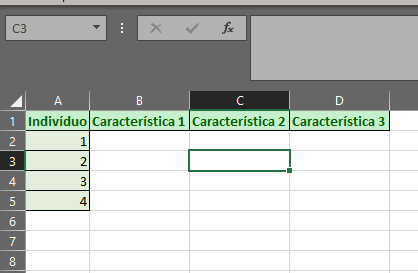
\includegraphics[width=1\textwidth,height=\textheight]{./figuras_tabulacao/excel1.png}

}

\caption{Tabulação das variáveis no excel}

\end{figure}

Cada uma das células receberá um valor \emph{x} referente a alguma
característica indicada pela coluna e um indivíduo representado pela
linha, em nosso caso temos 3 características para cada uma das 4
observações.

\hypertarget{alguns-problemas-no-meio-do-caminho}{%
\section{Alguns problemas no meio do
caminho}\label{alguns-problemas-no-meio-do-caminho}}

É valido ressaltar que é possível se deparar com alguns problemas que
talvez possam vir a ser solucionados da maneira errada.

A forma como tabulamos nossos dados pode vir a ser um facilitar ou
empecilho em nossas análises, um belo exemplo é a forma citada
anteriormente de classificação dos dados ou transformação para que sejam
salvos em alguma outra categoria, como faixa etária ou idade.

Outro problema é quando trabalhamos com dados que possas vir a ter mais
de uma resposta. Por exemplo: Quais sintomas estava sentindo? O melhor a
se fazer nesse caso é criar uma coluna para cada um dos possíveis
sintomas.

\begin{figure}

{\centering 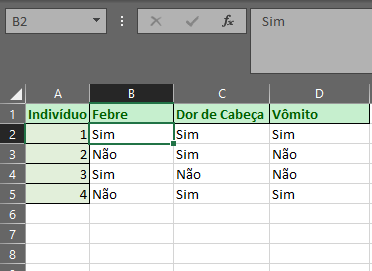
\includegraphics[width=1\textwidth,height=\textheight]{./figuras_tabulacao/excel2.png}

}

\caption{Mais de uma opção de escolha na variável}

\end{figure}

Uma outra forma seria:

\begin{figure}

{\centering 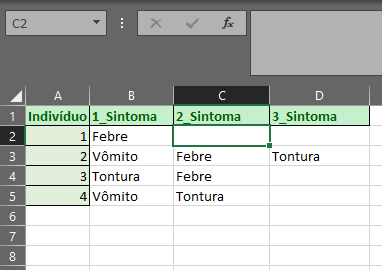
\includegraphics[width=1\textwidth,height=\textheight]{./figuras_tabulacao/excel3.png}

}

\caption{Mais de uma opção de escolha na variável, outra forma}

\end{figure}

Devemos lembrar sempre de anexar um \texttt{ID} ou forma de
identificação única para cada uma das observações. É possível criar uma
ou trabalhar com alguma já existente, um exemplo de uma já existente é o
próprio CPF ou RG quando trabalhamos com pessoas.

Vale ressaltar outras boas práticas ao realizar a tabulação:

\begin{itemize}
\item
  Se trabalhando com Excel ou Softwares parecidos, deixe a planilha
  apenas com a tabela de dados, evite armazenar na mesma planilha várias
  informações avulssas que não façam parte da sua tabela;
\item
  No R conseguimos especificar qual planilha de um arquivo
  \texttt{.xlsx} queremos transferir, porém pode vir a ser um pouco
  confuso as vezes, então é sugerido deixar todas as suas informações em
  uma única tabela em uma única planilha;
\item
  Padronização é extremamente importante, salve todos os dados para cada
  coluna em apenas um determinado formato (Ex.: Coluna Idade -
  \emph{Integer}, Coluna Raça - \emph{Character}), lembrando sempre de
  manter um padrão de medida (cm, L), variáveis do tipo categórico
  tambem precisam de padronização (Evite coisas como: Não, nao, n, N,
  não);
\item
  Cuidado ao classificar dados faltantes, uma prática errada é preencher
  esses dados com 0, isso pode vir a atrapalhar toda sua análise
\item
  Foi citado CPF como forma de identificação, mas pode haver casos em
  que teremos mais de uma linha contendo um mesmo indivíduo dependendo
  do nosso tipo de dados. Ou seja, esteja atento para que não haja
  duplicidade de variável identificadora ou \texttt{ID}.
\end{itemize}

\bookmarksetup{startatroot}

\hypertarget{anuxe1lise-exploratuxf3ria-dos-dados}{%
\chapter{Análise exploratória dos
dados}\label{anuxe1lise-exploratuxf3ria-dos-dados}}

Após o tratamento de uma base de dados, em geral, temos o interesse em
examinar e estudar as características de cada uma das variáveis
presentes no banco, de forma a identificar comportamentos e relações
entre as variáveis. Morettin e Singer (2020) apresentam um conjunto de
questões que normalmente se tenta responder ao se realizar uma análise
dos dados, sendo elas:

\begin{enumerate}
\def\labelenumi{\roman{enumi}.}
\item
  qual a frequência com que cada valor aparece no conjunto de dados ou
  seja, qual a distribuição de frequências dos dados?
\item
  quais são alguns valores típicos do conjunto de dados, como mínimo e
  máximo?
\item
  qual seria um valor para representar a posição (ou localização)
  central do conjunto de dados?
\item
  qual seria uma medida da variabilidade ou dispersão dos dados?
\item
  existem valores atípicos ou discrepantes (\(outliers\)) no conjunto de
  dados?
\item
  os dados podem ser considerados simétricos?
\end{enumerate}

Para responder a essas questões, fazemos uso de um conjunto de técnicas
numéricas e gráficas que nos permitem detectar padrões, resumir
informação e apresentar visivelmente características das variáveis de um
conjunto de dados. A essa metodologia denominamos análise descritiva ou
análise exploratória de dados e será objeto de estudo desse capítulo.
Para ilustrar as técnicas apresentadas, vamos realizar a análise
descritiva de algumas das variáveis presentes no banco de dados de
COVID-19 em gestantes e puérperas já devidamente tratadas no capítulo
anterior.

A decisão por qual técnica empregar para a análise descritiva de uma
variável, passa por qualificar corretamente a natureza da variável em
estudo em qualitativa nominal, qualitativa ordinal, quantitativa
discreta ou quantitativa contínua. Maiores detalhes sobre essa teoria
podem ser vistos na Seção XX.

Uma das principais ferramentas de resumo de informações de variáveis
qualitativas é a organização tabular que fornece a distribuição de
frequências de cada variável, conforme apresentado na Seção XX.

Em se tratando de variáveis quantitativas, utilizar uma tabela de
frequências para resumir informações da variável, especialmente nos
casos de variáveis contínuas, pode não ser a melhor estratégia, visto
que é comum obter frequências muito pequenas (em geral, 1) para os
diferentes valores da variável, não atingindo o propósito de resumir a
informação. Nesse sentido, vamos apresentar aqui medidas-resumo que
podem ser utilizadas para variáveis quantitativas.

\hypertarget{medidas-resumo}{%
\section{Medidas-resumo}\label{medidas-resumo}}

Uma medida-resumo é uma construção matemático/estatística que tenta
capturar em um único número um comportamento presente nos dados. Quatro
grandes grupos de medidas podem ser considerados para resumir variáveis
quantitativas, são elas: posição, dispersão, assimetria e curtose.
Vejamos agora que medidas são essas e como interpretá-las.

\hypertarget{medidas-de-posiuxe7uxe3o}{%
\subsection{Medidas de posição}\label{medidas-de-posiuxe7uxe3o}}

As medidas de posição, como o nome diz, indicam posições de interesse de
valores da variável. Por exemplo, se idade é a variável de interesse
investigada em um grupo de pessoas, e se quer trazer um informação
resumida dela no grupo, apresentar a menor e a maior idade encontrada,
valores típicos da idade no grupo, são exemplos de medidas de posição.

De maneira geral, vamos explorar aqui as seguintes medidas posição:
valor mínimo, valor máximo, percentis e medidas de tendência central,
tais como moda, média e mediana. Os valores mínimo e máximo de uma
variável quantitativa estão relacionados, respectivamente, com o menor e
o maior valor observado da variável analisada.

Medidas que buscam descrever um valor típico que a variável apresenta
são chamados de medidas de tendência ou posição central. Mas o que seria
uma valor típico? Como podemos definir isso? A resposta não é única e,
por isso, existem diferentes medidas de tendência central. Por exemplo,
se o valor típico considerado for aquele que mais se repete no conjunto
de dados para variável, o que temos é a moda. Se o valor típico for
aquele que ocupa uma posição central no conjunto de dados, de tal forma
que 50\% dos dados observados estão abaixo desse valor e os demais 50\%
estão acima, o que temos é a mediana. Agora, se o valor típico
considerado for pensado como um ponto de equilíbrio das observações da
variável, então temos a média.

Por definição, a medida estatística moda corresponde aos(s) valor(es)
mais frequente(s) do conjunto de dados observados para uma variável.
Conjunto de dados que não apresentam valores repetidos são considerados
amodais. Um conjunto de dados é bimodal se tiver duas modas, indicando
que não apenas um único valor, mas dois valores do conjunto de dados
apresentam frequências igualmente mais altas que os demais valores.
Usando de mesmo raciocínio, havendo três ou mais valores modais em um
conjunto de dados, dizemos que o conjunto de dados é trimodal ou
multimodal, respectivamente. Vale citar que a moda também pode ser
obtida para variáveis qualitativas.

A média é a medida obtida ao somar todos os valores da variável e
dividí-la pela quantidade de dados observados. Matematicamente,
considere \(x_1\), \(x_2\), \ldots, \(x_n\) as observações de uma
variável \(X\), assim a média é definida como:

\begin{equation}
\bar{x} = \frac{\sum_{i = 1}^n x_i}{n}.
\end{equation}

Para entender essa medida como ponto de equilíbrio, vamos representar
cada valor observado como pesos de mesma massa e distribuí-los sobre uma
reta de massa desprezível nas posições referentes aos valores da
variável em questão. Nosso objetivo agora é encontrar um ponto de apoio
nessa reta de tal forma que ela e os pesos corretamente posicionados
nela fiquem perfeitamente equilibrados, similar a uma balança. A média é
o único local em que se pode localizar o ponto de apoio na reta de forma
a obter um perfeito equilíbrio da reta e dos pesos. Para ilustrar essa
ideia, apresentamos a seguir uma representação gráfica considerando o
subconjunto da variável idade \{22, 28, 29, 34, 34, 35, 36, 36, 37,
39\}, cuja média é 33.

\begin{figure}

\begin{minipage}[t]{\linewidth}

{\centering 

\raisebox{-\height}{

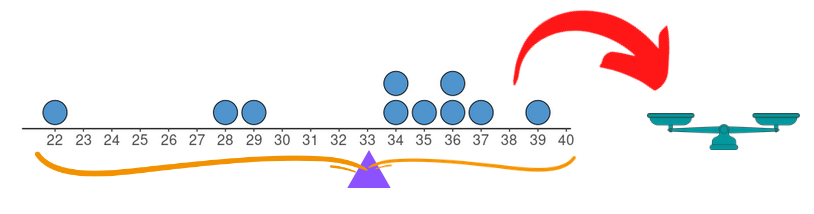
\includegraphics{./figuras_descritiva/Media_eq.png}

}

\caption{(a) Ponto de equilíbrio na média}

}

\end{minipage}%
\newline
\begin{minipage}[t]{\linewidth}

{\centering 

\raisebox{-\height}{

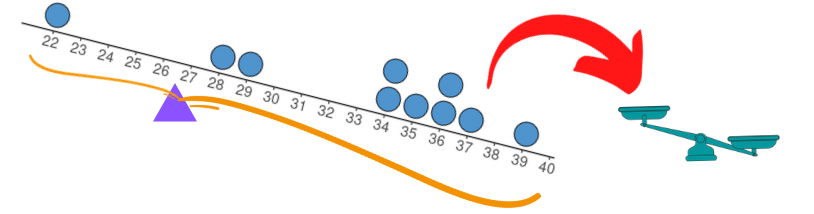
\includegraphics{./figuras_descritiva/Media_des.png}

}

\caption{(b) Ponto de equilíbrio fora da média}

}

\end{minipage}%

\caption{\label{fig-medias}Apresentando a média como ponto de
equilíbrio}

\end{figure}

No início dessa seção, apresentamos a noção intuitiva do que representa
o valor mediano, mas não como obtê-lo formalmente. A construção dessa
medida passa por organizar os dados de maneira crescente e calcular a
posição central dos dados via \(\frac{n+1}{2}\), em que \(n\) representa
o tamanho do conjunto de dados relacionada a variável de interesse. O
valor mediano é o valor na amostra ordenada que ocupa a posição
\(\frac{n+1}{2}\).

Quando \(n\) é ímpar, a expressão \(\frac{n+1}{2}\) vai sempre gerar um
valor inteiro, facilitando a obtenção da mediana. Por exemplo, o
subconjunto a seguir é formado por nove valores retirados da variável
idade, sendo eles: 21, 28, 24, 22, 31, 26, 22, 38, 16.

Ordenando esse subconjunto, obtemos 16, 21, 22, 22, 24, 26, 28, 31, 38.

Como \(n=9\), a posição em que se encontra a mediana será
\(\frac{9+1}{2}=5\). Assim, a mediana será 24, pois é o valor que está
na quinta posição do subconjunto ordenado.

Se \(n\) é par, a expressão \(\frac{n+1}{2}\) gerará um valor não
inteiro que apresenta apenas uma única casa decimal após a vírgula igual
a 5. Por exemplo, se a variável idade apresenta apenas 8 valores então
\(n = 8\) e a posição em que a mediana está localizada é dada por
\(\frac{n+1}{2} = \frac{8+1}{2} = 4,5\). Como inferir um valor para a
mediana quando a posição que ela ocupa é decimal? Note que a posição
\(4,5\) está exatamente no meio das posições 4 e 5, então o valor
mediano será definido como a média entre os valores que ocupam as
posições 4 e 5.

O subconjunto abaixo também consiste de valores retirados da variável
idade, porém note que nesse exemplo há 8 valores, ou seja, \(n=8\).

\[ 27, 16, 31, 43, 26, 42, 17, 40. \]

Ao ordenarmos, temos:

\[ 16, 17, 26, 27, 31, 40, 42, 43. \]

A mediana será o valor que está na posição \(\frac{8+1}{2} = 4,5\).
Logo, visto que a mediana está entre os valores que ocupam a quarta e
quinta posição, corresponde à média entre esses valores, sendo
\(\frac{27+31}{2}=29\).

Com ideia correlata a mediana, podemos apresentar medidas de posição não
centrais, as quais denominamos quantis ou percentis. O percentil 20, por
exemplo, é o valor da variável em que 20\% das observações no conjunto
de dados apresentam valores menores ou iguais a ele. Por consequência,
as restantes 80\% das observações possuem valores acima do percentil 20.
De maneira geral, podemos definir o percentil de ordem \(p\) como o
valor da variável em que \(100p\%\) \((0 < p < 1)\) das observações
estão à sua esquerda, ou seja, são menores ou iguais que ele.

Alguns percentis destacam-se por serem muito utilizados na análise de
dados, não só numericamente como graficamente. Esses percentis são
conhecido como quartis e basicamente dividem o conjunto de dados em 4
partes de mesmo tamanho. O primeiro quartil (\(Q_1\)) é o percentil 25,
o segundo quartil (\(Q_2\)) é o percentil 50 e o terceiro quartil
(\(Q_3\)) é o percentil 75. Vale notar que o segundo quartil é a
mediana. De posse desses valores, como veremos mais a frente nesse
capítulo, iremos construir o gráfico do tipo \(boxplot\), bastante
utilizado na análise de dados da saúde.

Ainda com respeito aos percentis, outro termo comum na literatura é o
decil que refere-se a divisão em 10 partes de mesmo tamanho do conjunto
de dados associado a variável analisada. O primeiro decil, por exemplo,
é o percentil 10 e o sexto decil é o percentil 60.

Todas as medidas de posição aqui apresentadas tem em comum terem a mesma
unidade de medida dos valores da variável observada, o que traz bastante
interpretabilidade.

\hypertarget{medidas-de-dispersuxe3o}{%
\subsection{Medidas de dispersão}\label{medidas-de-dispersuxe3o}}

Por mais que as medidas de posição apresentadas sejam muito úteis na
análise dados, elas por si só não se bastam como medidas resumo das
observações de uma variável em um conjunto de dados. É possível
construir diferentes conjuntos de dados para uma mesma variável que
apresentam os mesmo valores de medida central (média, mediana e moda),
mas tem comportamentos absolutamente diferentes. Por exemplo, veja a
figura a seguir.

\begin{figure}

\begin{minipage}[t]{0.50\linewidth}

{\centering 

\raisebox{-\height}{

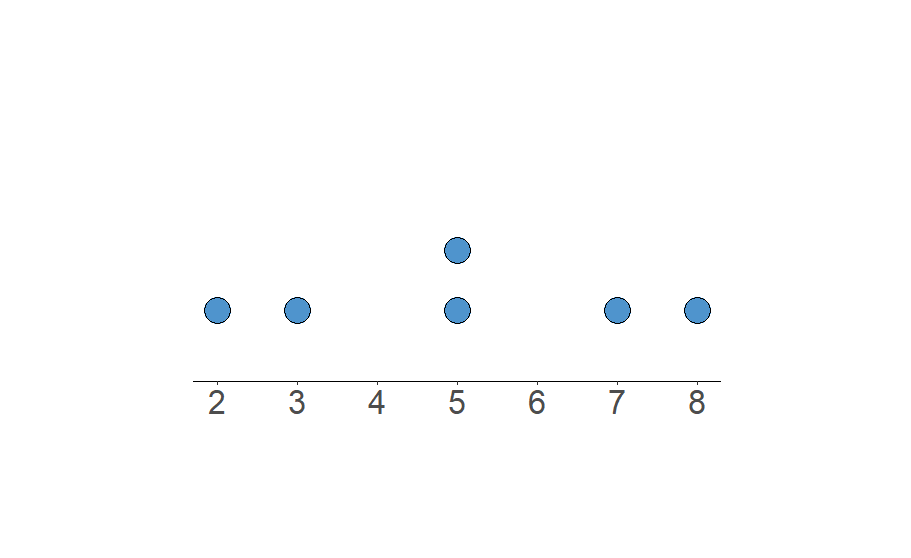
\includegraphics{./figuras_descritiva/plot1.png}

}

}

\subcaption{\label{fig-var1}Dados: 2 ,3, 5 , 5, 7, 8.}
\end{minipage}%
%
\begin{minipage}[t]{0.50\linewidth}

{\centering 

\raisebox{-\height}{

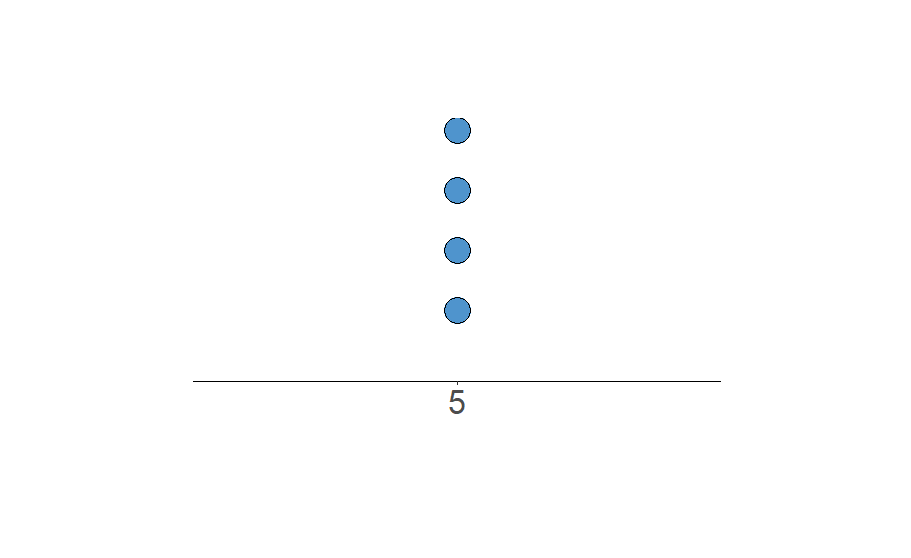
\includegraphics{./figuras_descritiva/plot2.png}

}

}

\subcaption{\label{fig-var2}Dados: 5,5,5,5.}
\end{minipage}%

\caption{\label{fig-var}Exemplos de conjuntos de dados com mesma média,
moda e mediana.}

\end{figure}

Os dois conjuntos de dados apresentam os mesmos valores de média,
mediana e moda. O que diferencia os dois conjuntos? O quão diferentes ou
parecidos são as observações entre si em cada conjunto da variável. Na
Figura Figura~\ref{fig-var2}, notamos que os quatro valores observados
são iguais entre si e que, portanto, as observações nesse conjunto não
variam, diferente do que ocorre para os dados que geraram o gráfico da
Figura Figura~\ref{fig-var1}. Medidas de dispersão ou variabilidade são
as medidas responsáveis por quantificar o quão diferente são os dados
entre si. De forma bastante intuitiva temos que se os dados observados
da variável não variam, então a medida de dispersão dela é zero e, caso
haja diferenças entre os valores observados, então essa medida vai ser
um valor positivo. Quanto maior a medida de variabilidade, mais
diferente são os dados observados da variável entre si.

Não existe uma única medida de dispersão na literatura, aqui vamos
considerar as seguintes medidas: amplitude, intervalo interquartil,
variância, desvio padrão e coeficiente de variação.

De fácil obtenção e interpretabilidade, a amplitude é a diferença entre
o valor máximo e o valor mínimo da variável analisada no conjunto de
dados e nos dá uma ideia do intervalo de variação dos dados. Uma
desvantagem é que essa medida é absolutamente influenciada pela presença
de valores discrepantes ou \(outliers\). O intervalo interquartil é uma
medida mais robusta do que a amplitude intervalar e é calculada como a
diferença entre o terceiro e o primeiro quartil, ou seja, é a amplitude
entre os 50\% dos dados centrais.

Por mais informativas que sejam as medidas de amplitude e intervalo
interquartil, queremos uma medida de dispersão que não considere apenas
dois valores da amostra (mínimo e máximo ou primeiro e terceiro quartis)
e sim todos os dados. Uma medida bastante intuitiva seria considerar a
soma dos desvios de cada uma das observações em torno da média. Mas aí
temos um problema: a soma dos desvios da média é sempre zero! Isso
acontece porque sempre há desvios positivos e negativos que quando
somados se anulam. Uma solução para essa questão é considerar alguma
função que considere apenas o valor do desvio e não o seu sinal. Uma
função candidata é a função quadrática (lembre que, por exemplo,
\((−2)^2=4\)). Nessa construção surge a variância: soma dos desvios
quadrados dividida pelo total de observações (\(n\)), ou seja, a média
dos desvios quadrados. Assim, a variância quantifica o quanto os dados
estão dispersos da média, em média.

Matematicamente, considere \(x_1\), \(x_2\), \ldots, \(x_n\) as
observações de uma variável \(X\) e \(\bar{x}\) a média observada dessa
variável. A variância seria calculada como:

\begin{equation}\protect\hypertarget{eq-var1}{}{
\mbox{Var(X)} = \frac{\sum_{i = 1}^n (x_i - \bar{x})^2}{n}.
}\label{eq-var1}\end{equation}

Por mais intuitiva que seja essa construção, programas como o R e
similares utilizam em sua análise uma versão modificada do cálculo da
variância acima apresentado, em que a soma dos desvios quadrados é
dividida por \(n-1\), não por \(n\). Justificativas para isso se devem a
propriedades inferenciais. A maioria dos conjuntos de dados considerados
nos estudos referem-se a análise de amostras de uma população e não a
análise de todos os elementos de uma população. Ao mesmo tempo, um dos
principais objetivos da análise estatística é fazer análises para a
população e não apenas para a amostra considerada no estudo.
Basicamente, se temos interesse de conhecer o valor médio de uma
variável na população (\(\mu\)), na impossibilidade de analisar todos os
elementos dela e obter a medida, o fazemos de forma aproximada
investigando o valor médio dessa variável na amostra (\(\bar{x}\)). Esse
mesmo raciocínio ocorre para a variância, na impossibilidade de obter a
variância da variável para todos os elementos da população
(\(\sigma^2\)), analisamos essa medida via amostra, o caso é que é
possível mostrar que para amostras de tamanho pequeno, a variância
apresentada em (Equação~\ref{eq-var1}) não aproxima-se bem do valor de
\(\sigma^2\). Matematicamente, é possível mostrar que tal dificuldade é
contornada fazendo uso do divisor igual a \(n-1\) em
(Equação~\ref{eq-var1}). Na literatura esse cálculo muitas vezes é
denominado como variância amostral e representado pelo símbolo \(S^2\)
de tal forma que

\begin{equation}\protect\hypertarget{eq-var2}{}{
S^2 = \frac{\sum_{i = 1}^n (x_i - \bar{x})^2}{n-1}.
}\label{eq-var2}\end{equation}

Vale ressaltar também que a medida que se considera tamanhos de amostra
maiores, calcular a variância com divisor \(n\) ou \(n-1\) torna-se
indiferente.

Como a unidade de medida da variância é o quadrado da unidade de medida
da variável correspondente, convém definir outra medida de dispersão que
mantenha a unidade de medida original. Uma medida com essa propriedade é
a raiz quadrada da variância, conhecida por desvio padrão.

Caso o interesse seja calcular e comparar a dispersão entre variáveis
com unidades dimensionais de natureza diferente, por exemplo,
comprimento (em metros) e massa (em kg), não convém utilizar as medidas
de dispersão apresentadas anteriormente pois todas as medidas
apresentadas carregam consigo a unidade de medida considerada para a
variável. Nesse caso, podemos fazer uso do coeficiente de variação (CV)
para cada uma das variáveis analisadas, já que o CV é uma medida de
dispersão relativa adimensional, calculada via razão entre o
desvio-padrão e a média observada para a variável e quanto maior o seu
valor, maior a dispersão dos dados em termos relativos a média.

\hypertarget{medidas-de-assimetria-e-curtose}{%
\subsection{Medidas de assimetria e
curtose}\label{medidas-de-assimetria-e-curtose}}

Além das medidas de posição e variabilidade, existe um conjunto de
medidas dedicadas a explorar a forma da distribuição de frequências dos
dados. Especificamente aqui estudaremos algumas: coeficientes de
assimetria e de curtose e variações destas.

Como boa parte dos estudos na área de saúde é realizado através de
amostras da variável de interesse na população, vamos precisar definir
os momentos amostrais centrais que serão ferramenta fundamental para a
construção dos coeficientes de assimetria, curtose e seus derivados. Por
definição, o momento amostral centrado (na média) de ordem \(r\) é dado
por

\[
m_r = \frac{\sum_{i = 1}^n (x_i - \bar{x})^r}{n}, \; r = 1, 2, \cdots.
\]

A versão populacional do momento centrado de ordem \(r\) é expressa por
\(\mu_r = \frac{\sum_{i = 1}^n (x_i - \mu)^r}{N}\), em que
\(r = 1, 2, \cdots \;\) e \(\mu\) e \(N\) referem-se, respectivamente, a
média da variável de interesse e a quantidade de elementos investigados
na população.

Dessa forma, o coeficiente de assimetria amostral é dado por
\(\frac{m_3}{m_2^{3/2}}\). Populações cuja a distribuição da variável é
simétrica apresentam coeficiente de assimetria igual a zero.
Distribuições assimétricas à direita apresentam valores positivos de
coeficiente de assimetria para a variável analisada populacionalmente,
assim como distribuições assimétricas à esquerda apresentam coeficiente
de assimetria negativo.

Analogamente, \(\frac{\mu_3}{\mu_2^{3/2}}\) é o coeficiente de
correlação populacional.

Populações cuja a distribuição da variável é simétrica apresentam
coeficiente de assimetria igual a zero. Distribuições assimétricas à
direita apresentam valores positivos de coeficiente de assimetria para a
variável analisada populacionalmente, assim como distribuições
assimétricas à esquerda apresentam coeficiente de assimetria negativo.

\begin{figure}

\begin{minipage}[t]{0.50\linewidth}

{\centering 

\raisebox{-\height}{

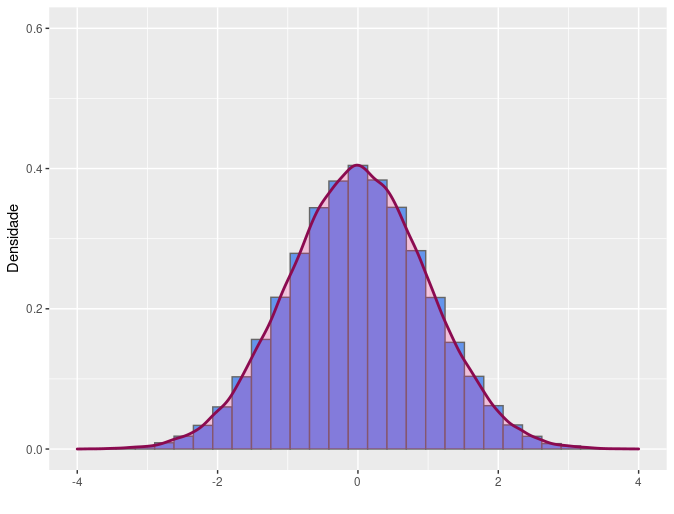
\includegraphics{./figuras_descritiva/Fig1_N2.png}

}

\caption{(a) Simétrico}

}

\end{minipage}%
%
\begin{minipage}[t]{0.50\linewidth}

{\centering 

\raisebox{-\height}{

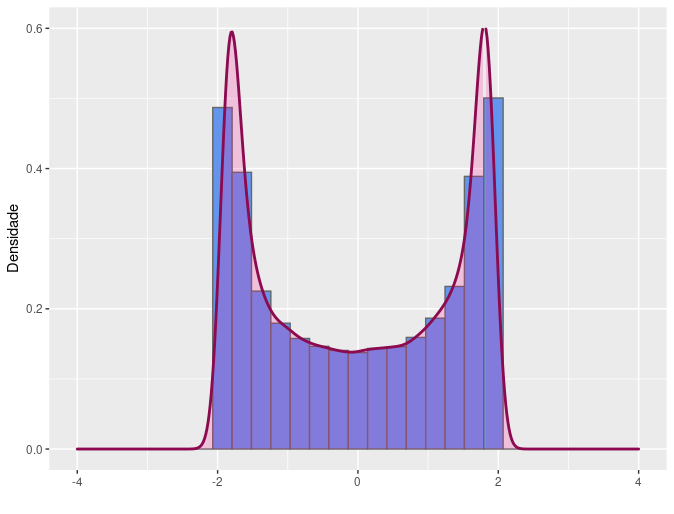
\includegraphics{./figuras_descritiva/Fig2_N2.png}

}

\caption{(b) Simétrico}

}

\end{minipage}%
\newline
\begin{minipage}[t]{0.50\linewidth}

{\centering 

\raisebox{-\height}{

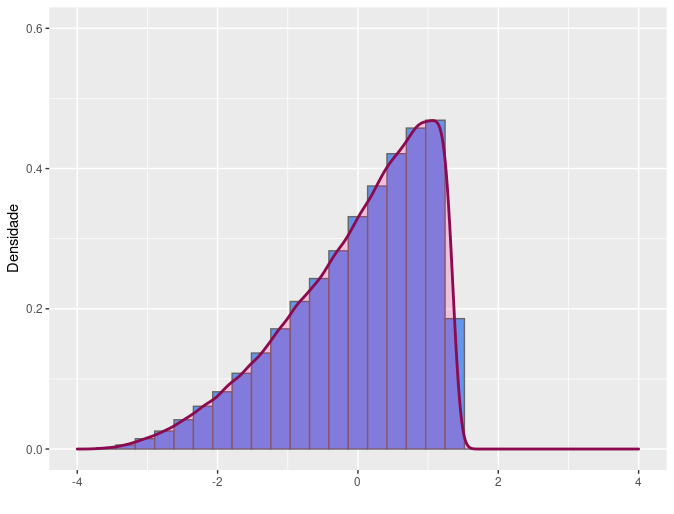
\includegraphics{./figuras_descritiva/Fig3_N2.png}

}

\caption{(c) Assimétrico à esquerda}

}

\end{minipage}%
%
\begin{minipage}[t]{0.50\linewidth}

{\centering 

\raisebox{-\height}{

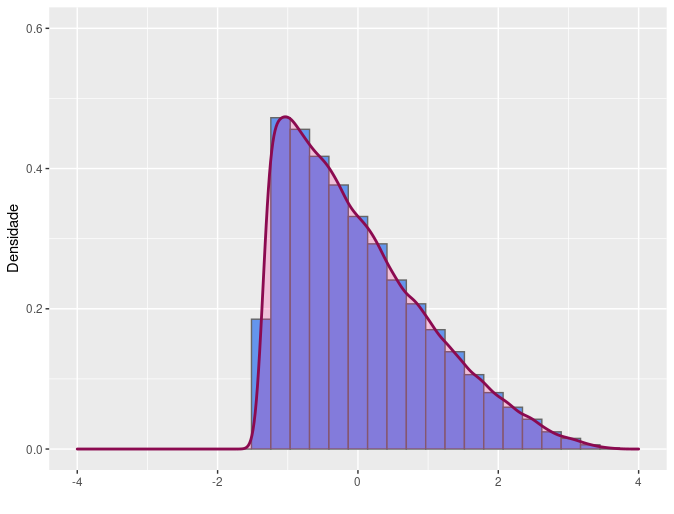
\includegraphics{./figuras_descritiva/Fig4_N2.png}

}

\caption{(d) Assimétrico à direita}

}

\end{minipage}%

\caption{\label{fig-assim}Histogramas e funções de densidade}

\end{figure}

Coeficientes de assimetria amostrais diferentes de zero devem ser
interpretados com cautela, uma vez que por se tratar de uma amostra não
significa que necessariamente o comportamento da variável na população
seja assimétrico. Testes estatísticos devem ser realizados para avaliar
a hipotese de simetria da variável na população.

Ainda com respeito a forma da distribuição da variável, podemos avaliar
o comportamento em suas caudas através do coeficiente de curtose
amostral que se define por \(\frac{m_4}{m_2^{2}}\). Distribuições de
variáveis com valor de curtose igual a 3 são denominadas mesocúrticas.
Tomada muitas vezes como referência, a distribuição normal apresenta
coeficiente de curtose igual a três. Distribuições com coeficiente de
curtose menores que 3 são denominadas platicúrticas e apresentam caudas
mais leves (``finas'') do que a da distribuição normal. Distribuições
com coeficiente de curtose maiores que 3 são denominadas leptocúrticas e
apresentam caudas mais pesadas (``grossas'') do que a da distribuição
normal. A distribuição t-Student é um exemplo de distribuição
leptocúrtica.

Na literatura é muito comum ser apresentado uma variante do coeficiente
de curtose denominada excesso de curtose. Esse excesso é avaliado em
relação a curtose do modelo normal por isso seu valor é calculado
fazendo o coeficiente de curtose subtraído de 3. Dessa forma, o excesso
de curtose em distribuições mesocúrticas é igual a zero, em
distribuições leptocúrticas é maior que zero e em distribuições
platicúrticas é menor que zero.

\begin{figure}

{\centering 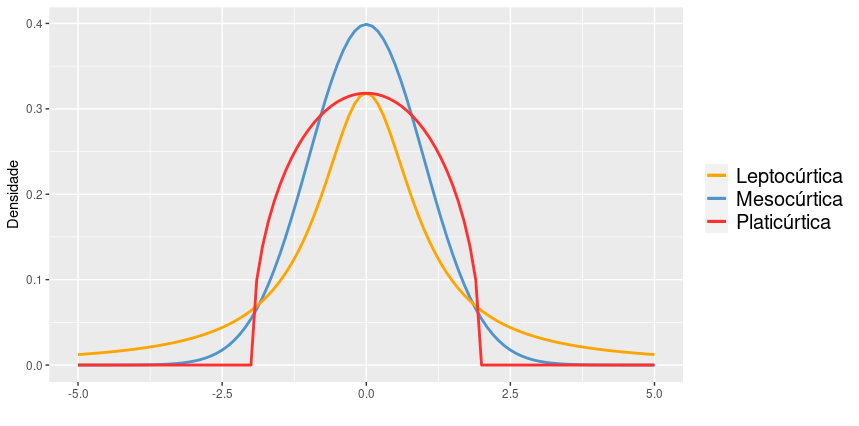
\includegraphics{./figuras_descritiva/Curtose.png}

}

\caption{\label{fig-Curto}Exemplo de funções de densidade com diferentes
medidas de curtose.}

\end{figure}

Ressalva similar feita ao coeficiente de assimetria deve ser considerado
para o coeficiente de curtose ou de excesso de curtose. Um coeficiente
de curtose amostral diferente de três ou, de forma equivalente, com
excesso de curtose amostral diferente de zero, não implica
necessariamente que a distribuição da variável na população possui
caudas mais leves ou mais pesadas do que a da distribuição normal. Para
que se possa fazer tal afirmação é necessária a realização de testes
estatísticos inferenciais. Os coeficientes amostrais de assimetria e
curtose tão somente nos dão uma medida da forma da distribuição de
frequências e \(insights\) do comportamento da variável na população,
que devem ser verificados via análise inferencial estatística.

No R, para obter essas medidas resumo vamos utilizar a função
\texttt{descr} também do pacote \texttt{summarytools}. No comando abaixo
pedimos ao R as medidas descritivas da variável quantitativa ``idade''.

\begin{Shaded}
\begin{Highlighting}[]
\FunctionTok{descr}\NormalTok{(dados}\SpecialCharTok{$}\NormalTok{idade)}
\end{Highlighting}
\end{Shaded}

\begin{verbatim}
Descriptive Statistics  
dados$idade  
N: 11523  

                       idade
----------------- ----------
             Mean      30.25
          Std.Dev       7.04
              Min      10.00
               Q1      25.00
           Median      30.00
               Q3      35.00
              Max      55.00
              MAD       7.41
              IQR      10.00
               CV       0.23
         Skewness       0.17
      SE.Skewness       0.02
         Kurtosis      -0.10
          N.Valid   11514.00
        Pct.Valid      99.92
\end{verbatim}

Note que os nomes de algumas das estatísticas apresentadas pela função
\texttt{descr} estão em inglês. \(Mean\) refere-se ao valor médio da
variável analisada, \(Std.Dev\) corresponde ao desvio-padrão, IQR é o
símbolo para o intervalo interquartil, MAD é o desvio-médio absoluto,
\(Skewness\) é o coeficiente de assimetria, \(SE.Skewness\) é o
erro-padrão do coeficiente de assimetria, \(Kurtosis\) é o coeficiente
de excesso de curtose e \(N.Valid\) e \(Pct.Valid\) correspondem,
respectivamente, ao número de observações válidas e seu percentual no
conjunto de dados considerado para a variável.

Especificamente para a variável idade, podemos notar que das 11523
observações, apenas 11514 (99.92 \%) foram consideradas válidas. Isso
acontece porque nesse conjunto de dados, 9 pessoas não declararam a
idade, ficando com a casela vazia (NA). Todas as medidas-resumo foram
calculadas considerando apenas as observações válidas. Sendo assim,
algumas análises que podem ser realizadas para a variável idade através
da função \texttt{descr} são que a idade média dentre as observações
válidas foi de 30,25 anos, com desvio-padrão de 7,04 anos. A menor idade
observada foi de 10 anos e a máxima foi de 55 anos. 50\% das mulheres
analisadas tem idade inferior a 30 anos (mediana) e 25\% delas tem idade
superior a 35 anos (Q3). O coeficiente de assimetria foi 0.17 (com
erro-padrão de 0.02), indicando que a distribuição de frequências da
variável idade é levemente assimétrica à direita. O coeficiente de
excesso de curtose foi -0.10 e o intervalo interquartil (Q3 - Q1) foi
10.

Se quiser que a tabela apresente apenas algumas medidas-resumo
pré-selecionadas, podemos informar ao R por meio do argumento
\texttt{stats}. Ainda, se quisermos que na tabela as medidas resumo
fiquem na coluna, usamos o argumento \texttt{transpose\ =\ TRUE}, como
segue:

\begin{Shaded}
\begin{Highlighting}[]
\FunctionTok{descr}\NormalTok{(dados}\SpecialCharTok{$}\NormalTok{idade,}\AttributeTok{stats =} \FunctionTok{c}\NormalTok{(}\StringTok{"min"}\NormalTok{, }\StringTok{"mean"}\NormalTok{, }\StringTok{"med"}\NormalTok{,}\StringTok{"sd"}\NormalTok{,}\StringTok{"max"}\NormalTok{), }\AttributeTok{transpose =} \ConstantTok{TRUE}\NormalTok{) }\CommentTok{\#sd é o desvio padrão (standard deviation)}
\end{Highlighting}
\end{Shaded}

\begin{verbatim}
Descriptive Statistics  
dados$idade  
N: 11523  

                Min    Mean   Median   Std.Dev     Max
----------- ------- ------- -------- --------- -------
      idade   10.00   30.25    30.00      7.04   55.00
\end{verbatim}

Caso se tenha interesse em apresentar a natureza da variável e um
\(preview\) gráfico da distribuição de frequências, podemos fazer uso da
função \texttt{dfSummary}. O argumento \texttt{method\ =\ "render"} para
a função \texttt{print} permite uma melhor apresentação visual dos
gráficos em documentos do tipo R \(Markdown\).

\begin{Shaded}
\begin{Highlighting}[]
\FunctionTok{print}\NormalTok{(}\FunctionTok{dfSummary}\NormalTok{(dados}\SpecialCharTok{$}\NormalTok{idade), }\AttributeTok{method =} \StringTok{"render"}\NormalTok{)}
\end{Highlighting}
\end{Shaded}

\begin{longtable}[]{@{}
  >{\centering\arraybackslash}p{(\columnwidth - 12\tabcolsep) * \real{0.1429}}
  >{\raggedright\arraybackslash}p{(\columnwidth - 12\tabcolsep) * \real{0.1429}}
  >{\raggedright\arraybackslash}p{(\columnwidth - 12\tabcolsep) * \real{0.1429}}
  >{\raggedright\arraybackslash}p{(\columnwidth - 12\tabcolsep) * \real{0.1429}}
  >{\raggedright\arraybackslash}p{(\columnwidth - 12\tabcolsep) * \real{0.1429}}
  >{\centering\arraybackslash}p{(\columnwidth - 12\tabcolsep) * \real{0.1429}}
  >{\centering\arraybackslash}p{(\columnwidth - 12\tabcolsep) * \real{0.1429}}@{}}
\toprule()
\begin{minipage}[b]{\linewidth}\centering
\textbf{No}
\end{minipage} & \begin{minipage}[b]{\linewidth}\centering
\textbf{Variable}
\end{minipage} & \begin{minipage}[b]{\linewidth}\centering
\textbf{Stats / Values}
\end{minipage} & \begin{minipage}[b]{\linewidth}\centering
\textbf{Freqs (\% of Valid)}
\end{minipage} & \begin{minipage}[b]{\linewidth}\centering
\textbf{Graph}
\end{minipage} & \begin{minipage}[b]{\linewidth}\centering
\textbf{Valid}
\end{minipage} & \begin{minipage}[b]{\linewidth}\centering
\textbf{Missing}
\end{minipage} \\
\midrule()
\endhead
1 & idade {[}numeric{]} & \begin{minipage}[t]{\linewidth}\raggedright
\begin{longtable}[]{@{}l@{}}
\toprule()
\endhead
Mean (sd) : 30.2 (7) \\
min ≤ med ≤ max: \\
10 ≤ 30 ≤ 55 \\
IQR (CV) : 10 (0.2) \\
\bottomrule()
\end{longtable}
\end{minipage} & 46 distinct values & & 11514 (99.9\%) & 9 (0.1\%) \\
\bottomrule()
\end{longtable}

Além do gráfico, uma informação adicional apresentada é que as 11514
observações válidas da variável idade estão distribuídas em 46 distintos
valores.

Outro pacote bastante interessante para medidas descritivas é o
\texttt{modelsummary}. Destacamos algumas funções desse pacote:

\begin{itemize}
\item
  datasummary\_skim: retorna as medidas descritivas das variáveis do
  banco de dados a depender do tipo identificado no argumento
  \texttt{type=\ (categorical\ ou\ numeric)};
\item
  datasummary: retorna as medidas descritivas das variáveis a depender
  de como monta os argumentos da função, permitindo retornar as medidas
  descritivas das variáveis quantitativas de interesse por categorias de
  outra(s) variável(is).
\end{itemize}

Para explorar a funcionalidade desse pacote e suas funções, vamos
filtrar o banco de dados original considerando apenas as informações das
mulheres gestantes e puérperas internadas em UTI.

\begin{Shaded}
\begin{Highlighting}[]
\NormalTok{dados\_uti }\OtherTok{\textless{}{-}}\NormalTok{ dados[}\SpecialCharTok{!}\FunctionTok{is.na}\NormalTok{(dados}\SpecialCharTok{$}\NormalTok{dias\_uti),]}
\end{Highlighting}
\end{Shaded}

Vamos selecionar algumas variáveis do banco de dados \texttt{dados\_uti}
e organizá-las em um novo \(data.frame\).

\begin{Shaded}
\begin{Highlighting}[]
\FunctionTok{library}\NormalTok{(dplyr)}
\NormalTok{dados\_uti\_res }\OtherTok{\textless{}{-}} \FunctionTok{select}\NormalTok{(dados\_uti,idade,cardiopati, faixa\_et, evolucao, dias\_uti)}
\end{Highlighting}
\end{Shaded}

Para esses dados, vamos fazer algumas análises via pacote
\texttt{modelsummary}. Assim,

\begin{Shaded}
\begin{Highlighting}[]
\FunctionTok{library}\NormalTok{(modelsummary)}
\end{Highlighting}
\end{Shaded}

Ao usar a função \texttt{datasummary\_skim}, vamos obter as medidas
descritivas das variáveis quantitativas (argumento
\texttt{type\ =\ "numeric")} e das variáveis qualitativas (argumento
\texttt{type\ =\ "categorical")}, respectivamente:

\begin{Shaded}
\begin{Highlighting}[]
\FunctionTok{datasummary\_skim}\NormalTok{(dados\_uti\_res,}
  \AttributeTok{type =} \StringTok{"numeric"}\NormalTok{,}
  \AttributeTok{histogram =} \ConstantTok{FALSE}\NormalTok{)}
\end{Highlighting}
\end{Shaded}

\begin{table}
\centering
\begin{tabular}[t]{lrrrrrrr}
\toprule
  & Unique (\#) & Missing (\%) & Mean & SD & Min & Median & Max\\
\midrule
idade & 42 & 0 & \num{31.2} & \num{6.6} & \num{10.0} & \num{31.0} & \num{55.0}\\
dias\_uti & 75 & 0 & \num{12.0} & \num{13.7} & \num{0.0} & \num{8.0} & \num{200.0}\\
\bottomrule
\end{tabular}
\end{table}

\begin{Shaded}
\begin{Highlighting}[]
\FunctionTok{datasummary\_skim}\NormalTok{(dados\_uti\_res,}
  \AttributeTok{type =} \StringTok{"categorical"}\NormalTok{, }\AttributeTok{na.rm =} \ConstantTok{FALSE}\NormalTok{)}
\end{Highlighting}
\end{Shaded}

\begin{table}
\centering
\begin{tabular}[t]{llrr}
\toprule
  &    & N & \%\\
\midrule
cardiopati & sim & 182 & \num{7.8}\\
 & nao & 791 & \num{34.0}\\
 & ignorado & 17 & \num{0.7}\\
faixa\_et & <20 & 98 & \num{4.2}\\
 & >=34 & 908 & \num{39.1}\\
 & 20-34 & 1317 & \num{56.7}\\
 & NA & 1 & \num{0.0}\\
evolucao & cura & 1645 & \num{70.8}\\
 & obito & 623 & \num{26.8}\\
 & obito por outras causas & 7 & \num{0.3}\\
 & ignorado & 31 & \num{1.3}\\
\bottomrule
\end{tabular}
\end{table}

Como a variável faixa etária (\texttt{faixa\_et}) foi declarada como
fator, a função \texttt{datasummary\_skim} apresenta 1 valor NA,
indicando que apenas uma mulher que esteve em UTI não teve determinada
sua faixa etária/idade. Para que as demais variáveis categóricas
apresentem essa informação e não as deixe omitida, como no caso da
variável cardiopatia, vamos precisar declarar essas variáveis como
caracter e não como fator. Esse procedimento também será adotado para as
demais variáveis categóricas.

\begin{Shaded}
\begin{Highlighting}[]
\NormalTok{dados\_uti\_res}\SpecialCharTok{$}\NormalTok{cardiopati }\OtherTok{\textless{}{-}} \FunctionTok{as.character}\NormalTok{(dados\_uti\_res}\SpecialCharTok{$}\NormalTok{cardiopati)}
\NormalTok{dados\_uti\_res}\SpecialCharTok{$}\NormalTok{evolucao }\OtherTok{\textless{}{-}} \FunctionTok{as.character}\NormalTok{(dados\_uti\_res}\SpecialCharTok{$}\NormalTok{evolucao)}

\FunctionTok{datasummary\_skim}\NormalTok{(dados\_uti\_res,}
  \AttributeTok{type =} \StringTok{"categorical"}\NormalTok{, }\AttributeTok{na.rm =} \ConstantTok{FALSE}\NormalTok{)}
\end{Highlighting}
\end{Shaded}

\begin{table}
\centering
\begin{tabular}[t]{llrr}
\toprule
  &    & N & \%\\
\midrule
cardiopati & ignorado & 17 & \num{0.7}\\
 & nao & 791 & \num{34.0}\\
 & sim & 182 & \num{7.8}\\
 & NA & 1334 & \num{57.4}\\
faixa\_et & <20 & 98 & \num{4.2}\\
 & >=34 & 908 & \num{39.1}\\
 & 20-34 & 1317 & \num{56.7}\\
 & NA & 1 & \num{0.0}\\
evolucao & cura & 1645 & \num{70.8}\\
 & ignorado & 31 & \num{1.3}\\
 & obito & 623 & \num{26.8}\\
 & obito por outras causas & 7 & \num{0.3}\\
 & NA & 18 & \num{0.8}\\
\bottomrule
\end{tabular}
\end{table}

Uma das funções mais interessantes do pacote \texttt{modelsummary}é a
\texttt{datasummary}, pois ela nos permite analisar variáveis
quantitativas separada pelas categorias (grupos) de uma variável
qualitativa. Por exemplo, suponha que tenhamos interesse em analisar o
tempo de internação em UTI, estratificado pelos grupos faixa-etária e
evolução do caso, fazendo uso das seguintes medidas descritivas: média,
mediana, desvio padrão, mínimo, máximo e tamanho da amostra válido (sem
considerar observações faltantes para a variável em questão). O primeiro
passo é declarar as medidas-resumo de interesse como funções. O
argumento \texttt{na.rm\ =\ TRUE} indica que o cálculo da função deve
ser realizado excluindo os valores faltantes da variável.

\begin{Shaded}
\begin{Highlighting}[]
\NormalTok{media }\OtherTok{\textless{}{-}} \ControlFlowTok{function}\NormalTok{(x)   }\FunctionTok{mean}\NormalTok{(x, }\AttributeTok{na.rm =} \ConstantTok{TRUE}\NormalTok{)}
\NormalTok{mediana }\OtherTok{\textless{}{-}} \ControlFlowTok{function}\NormalTok{(x) }\FunctionTok{median}\NormalTok{(x, }\AttributeTok{na.rm =} \ConstantTok{TRUE}\NormalTok{)}
\NormalTok{dp }\OtherTok{\textless{}{-}} \ControlFlowTok{function}\NormalTok{(x) }\FunctionTok{sd}\NormalTok{(x, }\AttributeTok{na.rm =} \ConstantTok{TRUE}\NormalTok{)}
\NormalTok{minimo }\OtherTok{\textless{}{-}} \ControlFlowTok{function}\NormalTok{(x) }\FunctionTok{min}\NormalTok{(x, }\AttributeTok{na.rm =} \ConstantTok{TRUE}\NormalTok{)}
\NormalTok{maximo }\OtherTok{\textless{}{-}} \ControlFlowTok{function}\NormalTok{(x) }\FunctionTok{max}\NormalTok{(x, }\AttributeTok{na.rm =} \ConstantTok{TRUE}\NormalTok{)}
\NormalTok{n }\OtherTok{\textless{}{-}} \ControlFlowTok{function}\NormalTok{(x) }\FunctionTok{sum}\NormalTok{(}\SpecialCharTok{!}\FunctionTok{is.na}\NormalTok{(x))}
\end{Highlighting}
\end{Shaded}

\begin{Shaded}
\begin{Highlighting}[]
\FunctionTok{datasummary}\NormalTok{( (evolucao }\SpecialCharTok{+}\NormalTok{ faixa\_et) }\SpecialCharTok{\textasciitilde{}}
\NormalTok{              dias\_uti}\SpecialCharTok{*}\NormalTok{(n}\SpecialCharTok{+}\NormalTok{media}\SpecialCharTok{+}\NormalTok{dp}\SpecialCharTok{+}\NormalTok{minimo}\SpecialCharTok{+}\NormalTok{mediana}\SpecialCharTok{+}\NormalTok{maximo), }\AttributeTok{data =}\NormalTok{ dados\_uti\_res)}
\end{Highlighting}
\end{Shaded}

\begin{table}
\centering
\begin{tabular}[t]{llrrrrrr}
\toprule
  &    & n & media & dp & minimo & mediana & maximo\\
\midrule
evolucao & cura & \num{1645} & \num{10.78} & \num{12.01} & \num{0.00} & \num{6.00} & \num{107.00}\\
 & ignorado & \num{31} & \num{7.94} & \num{10.19} & \num{0.00} & \num{4.00} & \num{40.00}\\
 & obito & \num{623} & \num{15.18} & \num{15.46} & \num{0.00} & \num{12.00} & \num{200.00}\\
 & obito por outras causas & \num{7} & \num{51.71} & \num{64.62} & \num{2.00} & \num{25.00} & \num{183.00}\\
faixa\_et & <20 & \num{98} & \num{10.55} & \num{11.07} & \num{0.00} & \num{6.00} & \num{58.00}\\
 & >=34 & \num{908} & \num{12.91} & \num{14.66} & \num{0.00} & \num{8.00} & \num{200.00}\\
 & 20-34 & \num{1317} & \num{11.55} & \num{13.15} & \num{0.00} & \num{8.00} & \num{183.00}\\
\bottomrule
\end{tabular}
\end{table}

Agora veja como fica se eu considerar as medidas descritivas de mais de
uma variável quantitativas por duas variáveis qualitativas, selecionando
apenas as medidas descritivas, média, desvio-padrão e número de casos
observados:

\begin{Shaded}
\begin{Highlighting}[]
\FunctionTok{datasummary}\NormalTok{((evolucao }\SpecialCharTok{+}\NormalTok{ cardiopati)  }\SpecialCharTok{\textasciitilde{}}
\NormalTok{              (dias\_uti }\SpecialCharTok{+}\NormalTok{ idade)}\SpecialCharTok{*}\NormalTok{(n}\SpecialCharTok{+}\NormalTok{media}\SpecialCharTok{+}\NormalTok{dp), }\AttributeTok{data =}\NormalTok{ dados\_uti\_res)}
\end{Highlighting}
\end{Shaded}

\begin{table}
\centering
\begin{tabular}[t]{llrrrrrr}
\toprule
\multicolumn{2}{c}{ } & \multicolumn{3}{c}{dias\_uti} & \multicolumn{3}{c}{idade} \\
\cmidrule(l{3pt}r{3pt}){3-5} \cmidrule(l{3pt}r{3pt}){6-8}
  &    & n & media & dp & n & media & dp\\
\midrule
evolucao & cura & \num{1645} & \num{10.78} & \num{12.01} & \num{1645} & \num{31.05} & \num{6.57}\\
 & ignorado & \num{31} & \num{7.94} & \num{10.19} & \num{31} & \num{31.29} & \num{7.66}\\
 & obito & \num{623} & \num{15.18} & \num{15.46} & \num{622} & \num{31.61} & \num{6.70}\\
 & obito por outras causas & \num{7} & \num{51.71} & \num{64.62} & \num{7} & \num{32.14} & \num{7.65}\\
cardiopati & ignorado & \num{17} & \num{8.76} & \num{9.62} & \num{17} & \num{34.00} & \num{6.20}\\
 & nao & \num{791} & \num{12.74} & \num{13.30} & \num{791} & \num{30.96} & \num{6.82}\\
 & sim & \num{182} & \num{14.12} & \num{14.28} & \num{182} & \num{33.66} & \num{6.86}\\
\bottomrule
\end{tabular}
\end{table}

\hypertarget{tabelas-cruzadas---duas-variuxe1veis-qualitativas}{%
\section{Tabelas cruzadas - duas variáveis
qualitativas}\label{tabelas-cruzadas---duas-variuxe1veis-qualitativas}}

Tabelas cruzadas ou tabelas de contingência são tabelas que apresentam
frequências de duas ou mais variáveis qualitativas conjuntamente.

No R, para obter tabelas cruzadas, vamos utilizar a função ´ctable´
também do pacote ´summarytools´. No comando abaixo, pedimos ao R uma
tabela cruzada entre as variáveis qualitativas evolução
(\texttt{evolucao}) e faixa etária (\texttt{faixa\_et}) no banco de
dados otiginal.

\begin{Shaded}
\begin{Highlighting}[]
\FunctionTok{ctable}\NormalTok{(dados}\SpecialCharTok{$}\NormalTok{evolucao,}\AttributeTok{y=}\NormalTok{dados}\SpecialCharTok{$}\NormalTok{obesidade,}\AttributeTok{prop=}\StringTok{"t"}\NormalTok{)}
\end{Highlighting}
\end{Shaded}

Cross-Tabulation, Total Proportions\\
evolucao * obesidade\\
Data Frame: dados

\begin{longtable}[]{@{}lrrrrrr@{}}
\toprule()
\endhead
& obesidade & sim & nao & ignorado & & Total \\
evolucao & & & & & & \\
cura & & 555 (4.82\%) & 2897 (25.1\%) & 95 (0.82\%) & 5943 (51.58\%) &
9490 ( 82.4\%) \\
obito & & 199 (1.73\%) & 446 ( 3.9\%) & 14 (0.12\%) & 587 ( 5.09\%) &
1246 ( 10.8\%) \\
obito por outras causas & & 3 (0.03\%) & 13 ( 0.1\%) & 0 (0.00\%) & 6 (
0.05\%) & 22 ( 0.2\%) \\
ignorado & & 10 (0.09\%) & 71 ( 0.6\%) & 0 (0.00\%) & 206 ( 1.79\%) &
287 ( 2.5\%) \\
& & 23 (0.20\%) & 129 ( 1.1\%) & 4 (0.03\%) & 322 ( 2.79\%) & 478 (
4.1\%) \\
Total & & 790 (6.86\%) & 3556 (30.9\%) & 113 (0.98\%) & 7064 (61.30\%) &
11523 (100.0\%) \\
\bottomrule()
\end{longtable}

O argumento \texttt{prop} indica a forma como deve ser calculada a
proporção. Por padrão, a proporção é sempre calculada tendo-se como
referencial o total em linha, ou seja, \texttt{prop\ =\ "r"}. Outras
opções são \texttt{prop\ =\ "t"}, indicando que a proporção é em relação
ao número total de observações e \texttt{prop\ =\ "c"} se o referencial
for o total por coluna.

\begin{Shaded}
\begin{Highlighting}[]
\FunctionTok{ctable}\NormalTok{(dados}\SpecialCharTok{$}\NormalTok{evolucao,}\AttributeTok{y=}\NormalTok{dados}\SpecialCharTok{$}\NormalTok{obesidade,}\AttributeTok{prop=}\StringTok{"r"}\NormalTok{)}
\end{Highlighting}
\end{Shaded}

Cross-Tabulation, Row Proportions\\
evolucao * obesidade\\
Data Frame: dados

\begin{longtable}[]{@{}lrrrrrr@{}}
\toprule()
\endhead
& obesidade & sim & nao & ignorado & & Total \\
evolucao & & & & & & \\
cura & & 555 ( 5.8\%) & 2897 (30.5\%) & 95 (1.0\%) & 5943 (62.6\%) &
9490 (100.0\%) \\
obito & & 199 (16.0\%) & 446 (35.8\%) & 14 (1.1\%) & 587 (47.1\%) & 1246
(100.0\%) \\
obito por outras causas & & 3 (13.6\%) & 13 (59.1\%) & 0 (0.0\%) & 6
(27.3\%) & 22 (100.0\%) \\
ignorado & & 10 ( 3.5\%) & 71 (24.7\%) & 0 (0.0\%) & 206 (71.8\%) & 287
(100.0\%) \\
& & 23 ( 4.8\%) & 129 (27.0\%) & 4 (0.8\%) & 322 (67.4\%) & 478
(100.0\%) \\
Total & & 790 ( 6.9\%) & 3556 (30.9\%) & 113 (1.0\%) & 7064 (61.3\%) &
11523 (100.0\%) \\
\bottomrule()
\end{longtable}

\begin{Shaded}
\begin{Highlighting}[]
\FunctionTok{ctable}\NormalTok{(dados}\SpecialCharTok{$}\NormalTok{evolucao,}\AttributeTok{y=}\NormalTok{dados}\SpecialCharTok{$}\NormalTok{obesidade,}\AttributeTok{prop=}\StringTok{"c"}\NormalTok{)}
\end{Highlighting}
\end{Shaded}

Cross-Tabulation, Column Proportions\\
evolucao * obesidade\\
Data Frame: dados

\begin{longtable}[]{@{}lrrrrrr@{}}
\toprule()
\endhead
& obesidade & sim & nao & ignorado & & Total \\
evolucao & & & & & & \\
cura & & 555 ( 70.3\%) & 2897 ( 81.5\%) & 95 ( 84.1\%) & 5943 ( 84.13\%)
& 9490 ( 82.4\%) \\
obito & & 199 ( 25.2\%) & 446 ( 12.5\%) & 14 ( 12.4\%) & 587 ( 8.31\%) &
1246 ( 10.8\%) \\
obito por outras causas & & 3 ( 0.4\%) & 13 ( 0.4\%) & 0 ( 0.0\%) & 6 (
0.08\%) & 22 ( 0.2\%) \\
ignorado & & 10 ( 1.3\%) & 71 ( 2.0\%) & 0 ( 0.0\%) & 206 ( 2.92\%) &
287 ( 2.5\%) \\
& & 23 ( 2.9\%) & 129 ( 3.6\%) & 4 ( 3.5\%) & 322 ( 4.56\%) & 478 (
4.1\%) \\
Total & & 790 (100.0\%) & 3556 (100.0\%) & 113 (100.0\%) & 7064
(100.00\%) & 11523 (100.0\%) \\
\bottomrule()
\end{longtable}

Note que em todas as tabelas de contingência há a existência de linha e
coluna sem nome, isso acontece pois esta linha e/ou coluna está
resumindo os valores faltantes (NA). Por exemplo, a distribuição de
frequências da variável evolução para os que não preencheram o
\(status\) de obesidade nos diz que 5943 (84.13\%) foram curados, 587
(8.31\%) faleceram, 6 (0.08\%) viram a óbito por motivos outros que não
COVID-19, 206 (2.92\%) ignoraram essa informação (preencheram com 9) e
322 (4.56\%) deixaram em branco não só a informação da obesidade, mas
também o desfecho final da evolução. Para obter a tabela de contingência
apenas dos casos válidos simultâneos em ambas as variáveis, insira o
argumento \texttt{useNA\ =\ "no""}.

\begin{Shaded}
\begin{Highlighting}[]
\FunctionTok{ctable}\NormalTok{(dados}\SpecialCharTok{$}\NormalTok{evolucao,}\AttributeTok{y=}\NormalTok{dados}\SpecialCharTok{$}\NormalTok{obesidade, }\AttributeTok{prop=}\StringTok{"c"}\NormalTok{, }\AttributeTok{useNA =} \StringTok{"no"}\NormalTok{)}
\end{Highlighting}
\end{Shaded}

Cross-Tabulation, Column Proportions\\
evolucao * obesidade\\
Data Frame: dados

\begin{longtable}[]{@{}lrrrrr@{}}
\toprule()
\endhead
& obesidade & sim & nao & ignorado & Total \\
evolucao & & & & & \\
cura & & 555 ( 72.4\%) & 2897 ( 84.5\%) & 95 ( 87.2\%) & 3547 (
82.4\%) \\
obito & & 199 ( 25.9\%) & 446 ( 13.0\%) & 14 ( 12.8\%) & 659 (
15.3\%) \\
obito por outras causas & & 3 ( 0.4\%) & 13 ( 0.4\%) & 0 ( 0.0\%) & 16 (
0.4\%) \\
ignorado & & 10 ( 1.3\%) & 71 ( 2.1\%) & 0 ( 0.0\%) & 81 ( 1.9\%) \\
Total & & 767 (100.0\%) & 3427 (100.0\%) & 109 (100.0\%) & 4303
(100.0\%) \\
\bottomrule()
\end{longtable}

Caso não haja interesse em se apresentar as proporções, basta considerar
o argumento \texttt{prop="none"}, da seguinte forma:

\begin{Shaded}
\begin{Highlighting}[]
\FunctionTok{ctable}\NormalTok{(dados}\SpecialCharTok{$}\NormalTok{evolucao,}\AttributeTok{y=}\NormalTok{dados}\SpecialCharTok{$}\NormalTok{obesidade,}\AttributeTok{prop=}\StringTok{"none"}\NormalTok{)}
\end{Highlighting}
\end{Shaded}

Cross-Tabulation\\
evolucao * obesidade\\
Data Frame: dados

\begin{longtable}[]{@{}lrrrrrr@{}}
\toprule()
\endhead
& obesidade & sim & nao & ignorado & & Total \\
evolucao & & & & & & \\
cura & & 555 & 2897 & 95 & 5943 & 9490 \\
obito & & 199 & 446 & 14 & 587 & 1246 \\
obito por outras causas & & 3 & 13 & 0 & 6 & 22 \\
ignorado & & 10 & 71 & 0 & 206 & 287 \\
& & 23 & 129 & 4 & 322 & 478 \\
Total & & 790 & 3556 & 113 & 7064 & 11523 \\
\bottomrule()
\end{longtable}

Para tabelas de contingência com mais de duas variáveis, podemos adotar
o seguinte procedimento:

\begin{Shaded}
\begin{Highlighting}[]
\FunctionTok{with}\NormalTok{(dados, }\FunctionTok{stby}\NormalTok{(}\AttributeTok{data =} \FunctionTok{list}\NormalTok{(}\AttributeTok{x =}\NormalTok{ evolucao, }\AttributeTok{y =}\NormalTok{ obesidade), }
                   \AttributeTok{INDICES =}\NormalTok{ faixa\_et, }\AttributeTok{FUN =}\NormalTok{ ctable))}
\end{Highlighting}
\end{Shaded}

Cross-Tabulation, Row Proportions\\
evolucao * obesidade\\
Data Frame: dados\\
Group: faixa\_et = \textless20

\begin{longtable}[]{@{}lrrrrrr@{}}
\toprule()
\endhead
& obesidade & sim & nao & ignorado & & Total \\
evolucao & & & & & & \\
cura & & 12 (2.0\%) & 214 (35.0\%) & 2 (0.3\%) & 383 (62.7\%) & 611
(100.0\%) \\
obito & & 3 (6.5\%) & 22 (47.8\%) & 0 (0.0\%) & 21 (45.7\%) & 46
(100.0\%) \\
obito por outras causas & & 0 (0.0\%) & 2 (66.7\%) & 0 (0.0\%) & 1
(33.3\%) & 3 (100.0\%) \\
ignorado & & 0 (0.0\%) & 7 (20.0\%) & 0 (0.0\%) & 28 (80.0\%) & 35
(100.0\%) \\
& & 0 (0.0\%) & 2 (10.5\%) & 0 (0.0\%) & 17 (89.5\%) & 19 (100.0\%) \\
Total & & 15 (2.1\%) & 247 (34.6\%) & 2 (0.3\%) & 450 (63.0\%) & 714
(100.0\%) \\
\bottomrule()
\end{longtable}

Group: faixa\_et = \textgreater=34

\begin{longtable}[]{@{}lrrrrrr@{}}
\toprule()
\endhead
& obesidade & sim & nao & ignorado & & Total \\
evolucao & & & & & & \\
cura & & 231 ( 7.5\%) & 972 (31.5\%) & 37 (1.2\%) & 1842 (59.8\%) & 3082
(100.0\%) \\
obito & & 73 (13.9\%) & 182 (34.7\%) & 6 (1.1\%) & 263 (50.2\%) & 524
(100.0\%) \\
obito por outras causas & & 1 (12.5\%) & 6 (75.0\%) & 0 (0.0\%) & 1
(12.5\%) & 8 (100.0\%) \\
ignorado & & 1 ( 1.2\%) & 22 (25.9\%) & 0 (0.0\%) & 62 (72.9\%) & 85
(100.0\%) \\
& & 12 ( 7.4\%) & 44 (27.0\%) & 0 (0.0\%) & 107 (65.6\%) & 163
(100.0\%) \\
Total & & 318 ( 8.2\%) & 1226 (31.7\%) & 43 (1.1\%) & 2275 (58.9\%) &
3862 (100.0\%) \\
\bottomrule()
\end{longtable}

Group: faixa\_et = 20-34

\begin{longtable}[]{@{}lrrrrrr@{}}
\toprule()
\endhead
& obesidade & sim & nao & ignorado & & Total \\
evolucao & & & & & & \\
cura & & 310 ( 5.4\%) & 1710 (29.5\%) & 56 (1.0\%) & 3715 (64.2\%) &
5791 (100.0\%) \\
obito & & 123 (18.2\%) & 242 (35.9\%) & 8 (1.2\%) & 302 (44.7\%) & 675
(100.0\%) \\
obito por outras causas & & 2 (18.2\%) & 5 (45.5\%) & 0 (0.0\%) & 4
(36.4\%) & 11 (100.0\%) \\
ignorado & & 9 ( 5.4\%) & 42 (25.1\%) & 0 (0.0\%) & 116 (69.5\%) & 167
(100.0\%) \\
& & 11 ( 3.7\%) & 82 (27.9\%) & 4 (1.4\%) & 197 (67.0\%) & 294
(100.0\%) \\
Total & & 455 ( 6.6\%) & 2081 (30.0\%) & 68 (1.0\%) & 4334 (62.5\%) &
6938 (100.0\%) \\
\bottomrule()
\end{longtable}

\hypertarget{gruxe1ficos}{%
\section{Gráficos}\label{gruxe1ficos}}

Um gráfico pode ser a maneira mais adequada para resumir e apresentar um
conjunto de dados. Tem a vantagem de facilitar a compreensão de uma
determinada situação que queira ser descrita, permitindo uma
interpretação rápida e visual das suas principais características.

A visualização dos dados é uma etapa importantíssima da análise
estatística, pois é também a partir dela que criamos a intuição
necessária para escolher o teste ou modelo mais adequado para o nosso
problema.

\hypertarget{pacote-ggplot2}{%
\subsection{Pacote ggplot2}\label{pacote-ggplot2}}

Um pacote maravilhoso para gráficos no R é o \texttt{ggplot2}. A ideia
por trás desse pacote é um gráfico pode ser entendido como um mapeamento
dos dados a partir de atributos estéticos (cores, formas, tamanho) de
formas geométricas (pontos, linhas, barras).

\begin{Shaded}
\begin{Highlighting}[]
\FunctionTok{library}\NormalTok{(ggplot2)}
\end{Highlighting}
\end{Shaded}

\hypertarget{atributos-estuxe9ticos}{%
\subsubsection{Atributos estéticos}\label{atributos-estuxe9ticos}}

A função \texttt{aes} descreve como as variáveis são mapeadas em
aspectos visuais. Para isso, vamos precisar indicar qual variável será
representada no eixo x, qual será representada no eixo y, a cor e o
tamanho dos componentes geométricos, etc. de formas geométricas a serem
pré-definidas pelos geoms. A escolha da forma geométrica vai depender da
natureza das variáveis a serem analisadas e será discutido na sequencia.
Além disso, os aspectos que podem ou devem ser mapeados vão depender do
tipo de gráfico que estamos querendo construir. Basicamente, no pacote
´ggplot2´ temos as seguintes formas geométricas:

\begin{itemize}
\item
  geom\_point() gera gráficos de dispersão transformando pares (x,y) em
  pontos.
\item
  geom\_line: para retas definidas por pares (x,y);
\item
  geom\_abline: para retas definidas por um intercepto e uma inclinação;
\item
  geom\_hline: para retas horizontais;
\item
  geom\_bar: para barras;
\item
  geom\_histogram: para histogramas;
\item
  geom\_boxplot: para boxplots;
\item
  geom\_density: para densidades;
\item
  geom\_area: para áreas.
\end{itemize}

Para cada uma das formas geométricas podemos estabelecer aspectos
visuais que podem melhorar a visualização dos dados. Aspectos visuais
mais utilizados:

\begin{itemize}
\item
  color: altera a cor de formas que não têm área (pontos e retas);
\item
  fill: altera a cor de formas com área (barras, caixas, densidades,
  áreas);
\item
  size: altera o tamanho de formas;
\item
  type: altera o tipo da forma, geralmente usada para pontos;
\item
  linetype: altera o tipo da linha.
\end{itemize}

Para exemplificar os diferentes tipos de gráficos associando-os a
variáveis de diferentes naturezas, vamos considerar o banco de dados de
COVID-19 em gestantes e puérperas. De maneira geral, é necessário seguir
alguns passos gerais para a construção de qualquer gráfico via
\texttt{ggplot2}, a saber:

\begin{itemize}
\tightlist
\item
  Passo 1: sempre iniciar a construção chamando a função
  \texttt{ggplot}.
\item
  Passo 2: especificar na função \texttt{ggplot} o objeto que acomoda o
  banco de dados e apresenta a variável de interesse para a qual se quer
  fazer o gráfico. Esse objeto deve ser do tipo \(dataframe\).
\item
  Passo 3: informar as variáveis a serem consideradas no eixo horizontal
  e vertical via função \texttt{aes} e demais funções estéticas
  dependentes das variáveis.\\
\item
  Passo 4: informar o tipo de gráfico que se quer fazer (barra,
  histograma, \(boxplot\), etc).
\end{itemize}

\hypertarget{gruxe1ficos-para-variuxe1veis-qualitativas-e-quantitativas-discretas-com-poucos-valores-diferentes}{%
\subsubsection{Gráficos para variáveis qualitativas e quantitativas
discretas com poucos valores
diferentes}\label{gruxe1ficos-para-variuxe1veis-qualitativas-e-quantitativas-discretas-com-poucos-valores-diferentes}}

Um dos gráficos mais utilizados para a apresentação visual de variáveis
qualitativas e quantitativas discretas com poucas observações diferentes
é o gráfico de barras. Para construí-lo, é necessário utilizar no Passo
4 a função \texttt{geom\_bar}.\\
A seguir apresentamos um exemplo de gráfico de barras para a variável
qualitativa evolução dos casos relacionado a gestantes e puérperas
hospitalizadas por COVID-19.

\begin{Shaded}
\begin{Highlighting}[]
\FunctionTok{ggplot}\NormalTok{(dados, }\FunctionTok{aes}\NormalTok{(}\AttributeTok{x =}\NormalTok{ evolucao)) }\SpecialCharTok{+}
  \FunctionTok{geom\_bar}\NormalTok{(}\AttributeTok{fill =} \StringTok{"blue"}\NormalTok{) }\SpecialCharTok{+}
  \FunctionTok{labs}\NormalTok{(}\AttributeTok{x =} \StringTok{"Tipos de evolução"}\NormalTok{, }\AttributeTok{y =} \StringTok{"Número de casos"}\NormalTok{)}
\end{Highlighting}
\end{Shaded}

\begin{figure}[H]

{\centering 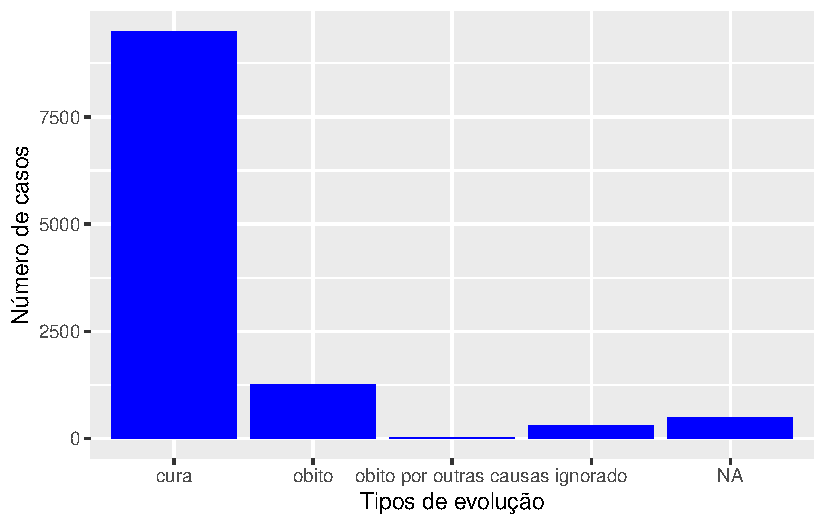
\includegraphics{./descritiva_files/figure-pdf/unnamed-chunk-22-1.pdf}

}

\end{figure}

Note que a função \texttt{labs} é responsável não só por inserir os
títulos nos eixos, como poder visto no gráfico anterior, mas também
títulos e subtítulos. Essa função pode ser sempre utilizada na
construção de gráficos via pacote \texttt{ggplot2}, independente do tipo
de gráfico a ser apresentado. Por exemplo,

\begin{Shaded}
\begin{Highlighting}[]
\FunctionTok{ggplot}\NormalTok{(dados, }\FunctionTok{aes}\NormalTok{(}\AttributeTok{x =}\NormalTok{ evolucao)) }\SpecialCharTok{+}
  \FunctionTok{geom\_bar}\NormalTok{(}\AttributeTok{fill =} \StringTok{"blue"}\NormalTok{) }\SpecialCharTok{+}
  \FunctionTok{labs}\NormalTok{(}\AttributeTok{x =} \StringTok{"Tipos de evolução"}\NormalTok{, }\AttributeTok{y =} \StringTok{"Número de casos"}\NormalTok{, }\AttributeTok{title =} \StringTok{"Evolução dos casos hospitalizados por COVID{-}19"}\NormalTok{, }\AttributeTok{subtitle =} \StringTok{"Mulheres gestantes e puérperas"}\NormalTok{)}
\end{Highlighting}
\end{Shaded}

\begin{figure}[H]

{\centering 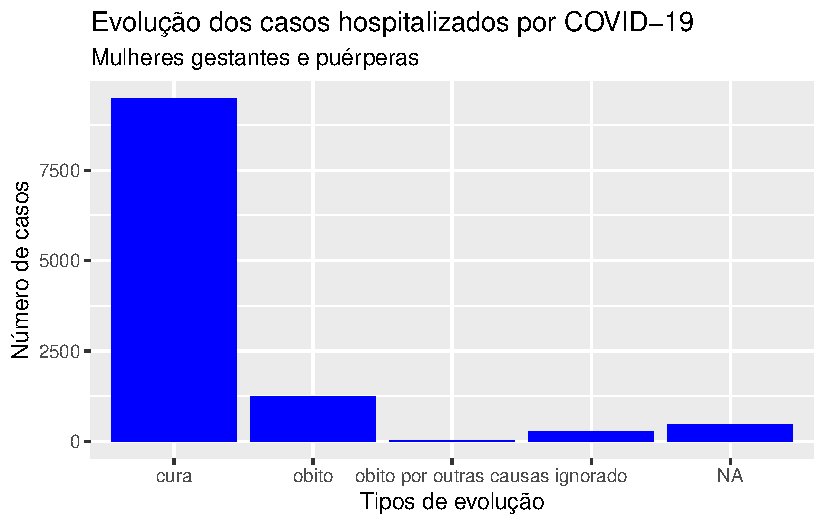
\includegraphics{./descritiva_files/figure-pdf/unnamed-chunk-23-1.pdf}

}

\end{figure}

No código a seguir apresentamos como apresentar as barras organizadas de
maneira decrescente. Note que há uma mudança na ordem das barras
referente a óbitos e óbitos por outras causas. Além disso, independente
da disposição escolhida para as barras, a categoria que representa as
mulheres que não tiveram sua evolução preenchida na notificação (NA)
sempre é apresentada como última barra, ainda que tenha uma alta
frequência em relação as outras categorias.

\begin{Shaded}
\begin{Highlighting}[]
\FunctionTok{ggplot}\NormalTok{(dados, }\FunctionTok{aes}\NormalTok{(}\AttributeTok{x =} \FunctionTok{reorder}\NormalTok{(evolucao, evolucao, }\ControlFlowTok{function}\NormalTok{(x)}\SpecialCharTok{{-}}\FunctionTok{length}\NormalTok{(x)))) }\SpecialCharTok{+}
  \FunctionTok{geom\_bar}\NormalTok{(}\AttributeTok{fill =} \StringTok{"blue"}\NormalTok{) }\SpecialCharTok{+}
  \FunctionTok{labs}\NormalTok{(}\AttributeTok{x =} \StringTok{"Tipos de evolução"}\NormalTok{, }\AttributeTok{y =} \StringTok{"Número de casos"}\NormalTok{, }\AttributeTok{title =} \StringTok{"Evolução dos casos hospitalizados por COVID{-}19"}\NormalTok{, }\AttributeTok{subtitle =} \StringTok{"Mulheres gestantes e puérperas"}\NormalTok{)}
\end{Highlighting}
\end{Shaded}

\begin{figure}[H]

{\centering 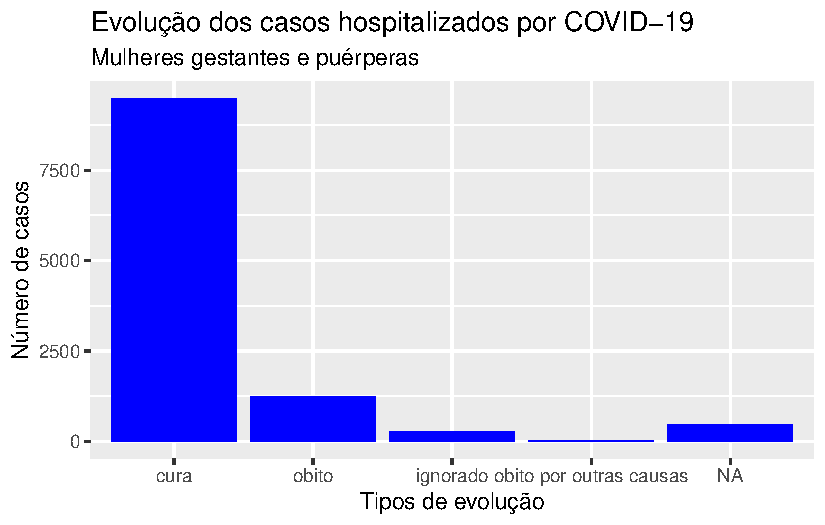
\includegraphics{./descritiva_files/figure-pdf/unnamed-chunk-24-1.pdf}

}

\end{figure}

Caso o interesse seja nas barras dispostas de maneira crescente, com
exceção do NA, basta reordenar a variável da seguinte forma:

\begin{Shaded}
\begin{Highlighting}[]
\FunctionTok{ggplot}\NormalTok{(dados, }\FunctionTok{aes}\NormalTok{(}\AttributeTok{x =} \FunctionTok{reorder}\NormalTok{(evolucao, evolucao, }\ControlFlowTok{function}\NormalTok{(x) }\FunctionTok{length}\NormalTok{(x)))) }\SpecialCharTok{+}
  \FunctionTok{geom\_bar}\NormalTok{(}\AttributeTok{fill =} \StringTok{"blue"}\NormalTok{) }\SpecialCharTok{+}
  \FunctionTok{labs}\NormalTok{(}\AttributeTok{x =} \StringTok{"Tipos de evolução"}\NormalTok{, }\AttributeTok{y =} \StringTok{"Número de casos"}\NormalTok{, }\AttributeTok{title =} \StringTok{"Evolução dos casos hospitalizados por COVID{-}19"}\NormalTok{, }\AttributeTok{subtitle =} \StringTok{"Mulheres gestantes e puérperas"}\NormalTok{)}
\end{Highlighting}
\end{Shaded}

\begin{figure}[H]

{\centering 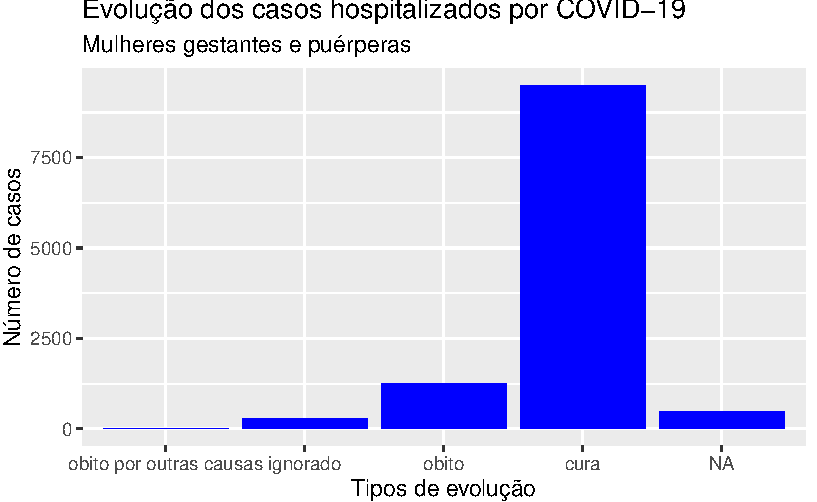
\includegraphics{./descritiva_files/figure-pdf/unnamed-chunk-25-1.pdf}

}

\end{figure}

A variável evolução (\texttt{evolucao}) pode ser classificada como
qualitativa nominal e, portanto, estamos livres para escolher a ordem
com que as categorias são apresentadas. Vamos ver agora o caso da
variável faixa-etária (\texttt{faixa\_et}) que, intrinsecamente, é uma
variável qualitativa ordinal. Se utilizássemos o mesmo código
considerado inicialmente para a variável evolução, obteríamos o seguinte
gráfico:

\begin{Shaded}
\begin{Highlighting}[]
\FunctionTok{ggplot}\NormalTok{(dados, }\FunctionTok{aes}\NormalTok{(}\AttributeTok{x =}\NormalTok{ faixa\_et)) }\SpecialCharTok{+}
  \FunctionTok{geom\_bar}\NormalTok{(}\AttributeTok{fill =} \StringTok{"purple"}\NormalTok{) }\SpecialCharTok{+}
  \FunctionTok{labs}\NormalTok{(}\AttributeTok{x =} \StringTok{"Faixa etária"}\NormalTok{, }\AttributeTok{y =} \StringTok{"Número de casos"}\NormalTok{, }\AttributeTok{title =} \StringTok{"Faixa etária das hospitalizadas por COVID{-}19"}\NormalTok{, }\AttributeTok{subtitle =} \StringTok{"Mulheres gestantes e puérperas"}\NormalTok{)}
\end{Highlighting}
\end{Shaded}

\begin{figure}[H]

{\centering 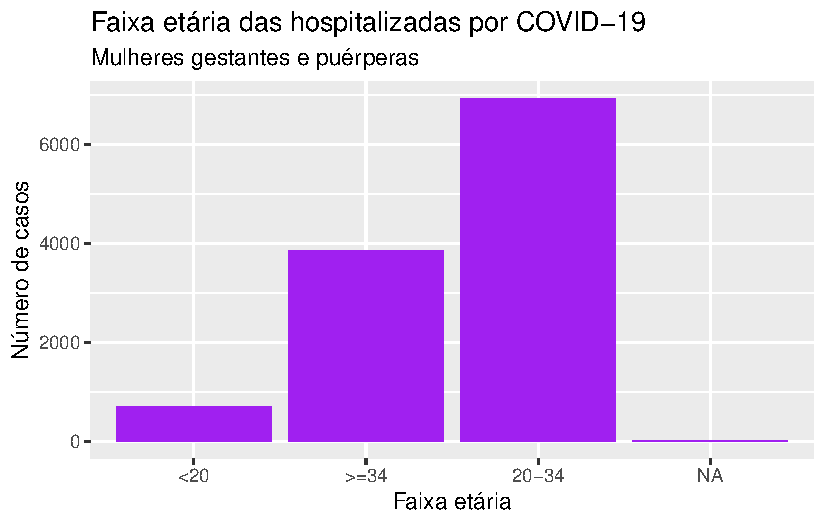
\includegraphics{./descritiva_files/figure-pdf/unnamed-chunk-26-1.pdf}

}

\end{figure}

Note que a barra para as mulheres com pelo menos 34 anos e a barra que
representa as mulheres com idade de 20 (incluso) a 34 anos estão em
posições trocadas, não respeitando a ordenação natural da variável.

\begin{Shaded}
\begin{Highlighting}[]
\CommentTok{\# Especificando a ordem dos níveis do fator }
\NormalTok{dados}\SpecialCharTok{$}\NormalTok{faixa\_et }\OtherTok{=} \FunctionTok{factor}\NormalTok{(dados}\SpecialCharTok{$}\NormalTok{faixa\_et, }\AttributeTok{levels =} \FunctionTok{c}\NormalTok{(}\StringTok{\textquotesingle{}\textless{}20\textquotesingle{}}\NormalTok{, }\StringTok{\textquotesingle{}20{-}34\textquotesingle{}}\NormalTok{, }\StringTok{\textquotesingle{}\textgreater{}=34\textquotesingle{}}\NormalTok{))}

\CommentTok{\# Gerando o gráfico}
\FunctionTok{ggplot}\NormalTok{(dados, }\FunctionTok{aes}\NormalTok{(}\AttributeTok{x =}\NormalTok{ faixa\_et)) }\SpecialCharTok{+}
  \FunctionTok{geom\_bar}\NormalTok{(}\AttributeTok{fill =} \StringTok{"purple"}\NormalTok{) }\SpecialCharTok{+}
  \FunctionTok{labs}\NormalTok{(}\AttributeTok{x =} \StringTok{"Faixa etária"}\NormalTok{, }\AttributeTok{y =} \StringTok{"Número de casos"}\NormalTok{, }\AttributeTok{title =} \StringTok{"Faixa etária das hospitalizadas por COVID{-}19"}\NormalTok{, }\AttributeTok{subtitle =} \StringTok{"Mulheres gestantes e puérperas"}\NormalTok{)}
\end{Highlighting}
\end{Shaded}

\begin{figure}[H]

{\centering 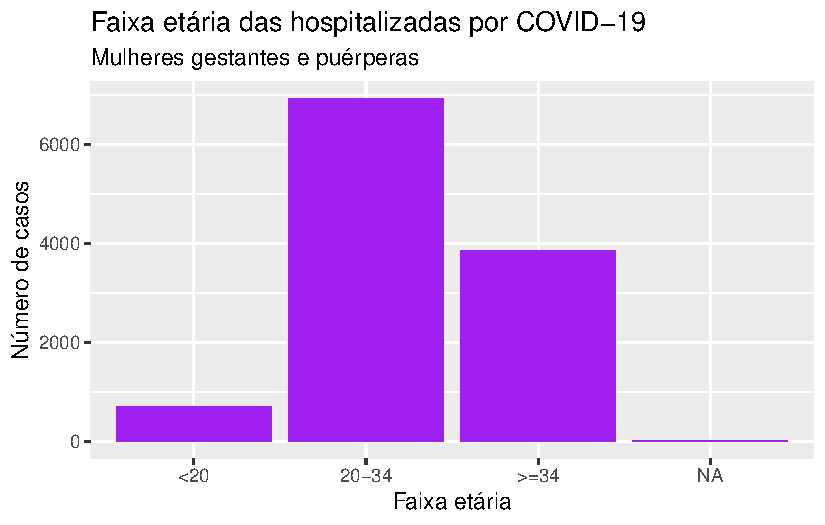
\includegraphics{./descritiva_files/figure-pdf/unnamed-chunk-27-1.pdf}

}

\end{figure}

Todos os gráficos de barra apresentados anteriormente apresentaram no
eixo vertical a contagem de indivíduos por categoria. vejamos agora o
código para apresentar o gráfico de barras com as frequências relativas.

\begin{Shaded}
\begin{Highlighting}[]
\FunctionTok{ggplot}\NormalTok{(dados, }\FunctionTok{aes}\NormalTok{(}\AttributeTok{x =}\NormalTok{ faixa\_et, }\AttributeTok{y =}\NormalTok{ (..count..)}\SpecialCharTok{/}\FunctionTok{sum}\NormalTok{(..count..))) }\SpecialCharTok{+}  
  \FunctionTok{geom\_bar}\NormalTok{(}\AttributeTok{fill=}\StringTok{"purple"}\NormalTok{) }\SpecialCharTok{+} 
  \FunctionTok{labs}\NormalTok{(}\AttributeTok{x =} \StringTok{"Faixa etária"}\NormalTok{, }\AttributeTok{y =} \StringTok{"Frequência relativa"}\NormalTok{, }\AttributeTok{title =} \StringTok{"Faixa etária das hospitalizadas por COVID{-}19"}\NormalTok{, }\AttributeTok{subtitle =} \StringTok{"Mulheres gestantes e puérperas"}\NormalTok{)}
\end{Highlighting}
\end{Shaded}

\begin{figure}[H]

{\centering 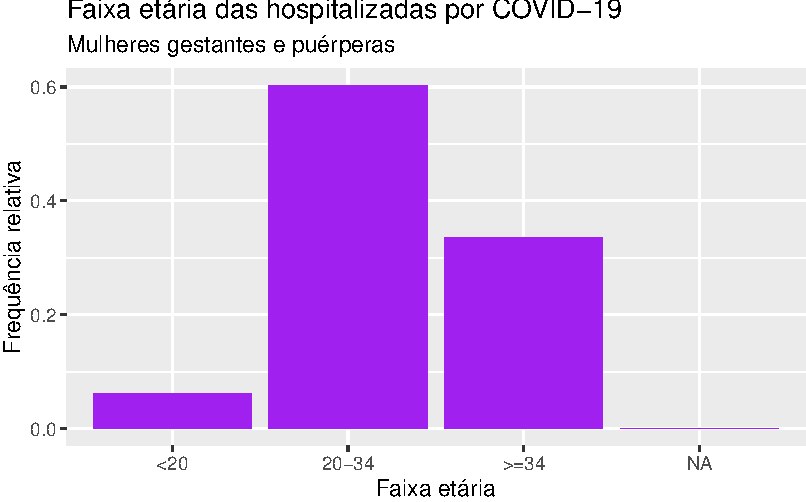
\includegraphics{./descritiva_files/figure-pdf/unnamed-chunk-28-1.pdf}

}

\end{figure}

Se o interesse é apresentar o gráfico em termos percentuais, basta
acrescentar a função \texttt{scale\_y\_continuous} com o argumento
\texttt{labels=scales::percent}.

\begin{Shaded}
\begin{Highlighting}[]
\FunctionTok{ggplot}\NormalTok{(dados, }\FunctionTok{aes}\NormalTok{(}\AttributeTok{x =}\NormalTok{ faixa\_et, }\AttributeTok{y =}\NormalTok{ (..count..)}\SpecialCharTok{/}\FunctionTok{sum}\NormalTok{(..count..))) }\SpecialCharTok{+}  
  \FunctionTok{geom\_bar}\NormalTok{(}\AttributeTok{fill=}\StringTok{"purple"}\NormalTok{) }\SpecialCharTok{+} 
  \FunctionTok{scale\_y\_continuous}\NormalTok{(}\AttributeTok{labels=}\NormalTok{scales}\SpecialCharTok{::}\NormalTok{percent) }\SpecialCharTok{+}
  \FunctionTok{labs}\NormalTok{(}\AttributeTok{x =} \StringTok{"Faixa etária"}\NormalTok{, }\AttributeTok{y =} \StringTok{"Porcentagem"}\NormalTok{, }\AttributeTok{title =} \StringTok{"Faixa etária das hospitalizadas por COVID{-}19"}\NormalTok{, }\AttributeTok{subtitle =} \StringTok{"Mulheres gestantes e puérperas"}\NormalTok{)}
\end{Highlighting}
\end{Shaded}

\begin{figure}[H]

{\centering 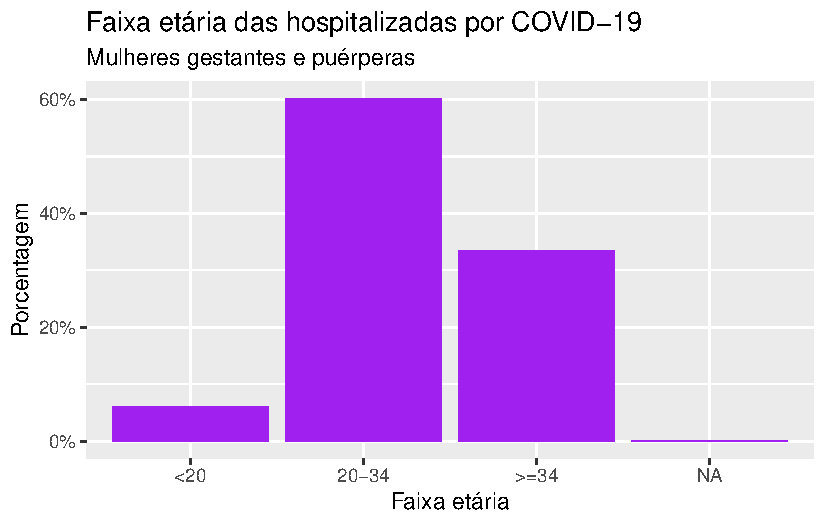
\includegraphics{./descritiva_files/figure-pdf/unnamed-chunk-29-1.pdf}

}

\end{figure}

Para inserir o percentual de cada categoria no gráfico, incluímos no
código anterior a função \texttt{geom\_text}, com o argumento
\texttt{lab} declarando o cálculo da frequência arredondado a duas casas
decimais. O argumento \texttt{vjust} indica a que altura se quer que o
texto com o percentual apareça no gráfico. Quanto mais negativo for o
valor, mais acima da barra estará o texto com o percentual. Se
\texttt{vjust\ =\ 0} apresenta o texto encima da barra e, quanto mais
positivo for o valor de \texttt{vjust} escolhido, mais interno da barra
ficará o texto.

\begin{Shaded}
\begin{Highlighting}[]
\FunctionTok{ggplot}\NormalTok{(dados, }\FunctionTok{aes}\NormalTok{(}\AttributeTok{x =}\NormalTok{ faixa\_et, }\AttributeTok{y =}\NormalTok{ (..count..)}\SpecialCharTok{/}\FunctionTok{sum}\NormalTok{(..count..))) }\SpecialCharTok{+}  
  \FunctionTok{geom\_bar}\NormalTok{(}\AttributeTok{fill=}\StringTok{"purple"}\NormalTok{) }\SpecialCharTok{+} 
  \FunctionTok{geom\_text}\NormalTok{(}\FunctionTok{aes}\NormalTok{(}\AttributeTok{label =} \FunctionTok{round}\NormalTok{((((..count..)}\SpecialCharTok{/}\FunctionTok{sum}\NormalTok{(..count..))}\SpecialCharTok{*}\DecValTok{100}\NormalTok{), }\DecValTok{2}\NormalTok{)), }\AttributeTok{stat=} \StringTok{"count"}\NormalTok{, }\AttributeTok{vjust =} \SpecialCharTok{{-}}\FloatTok{0.1}\NormalTok{)}\SpecialCharTok{+}
  \FunctionTok{scale\_y\_continuous}\NormalTok{(}\AttributeTok{labels=}\NormalTok{scales}\SpecialCharTok{::}\NormalTok{percent) }\SpecialCharTok{+}
  \FunctionTok{labs}\NormalTok{(}\AttributeTok{x =} \StringTok{"Faixa etária"}\NormalTok{, }\AttributeTok{y =} \StringTok{"Porcentagem"}\NormalTok{, }\AttributeTok{title =} \StringTok{"Faixa etária das hospitalizadas por COVID{-}19"}\NormalTok{, }\AttributeTok{subtitle =} \StringTok{"Mulheres gestantes e puérperas"}\NormalTok{)}
\end{Highlighting}
\end{Shaded}

\begin{figure}[H]

{\centering 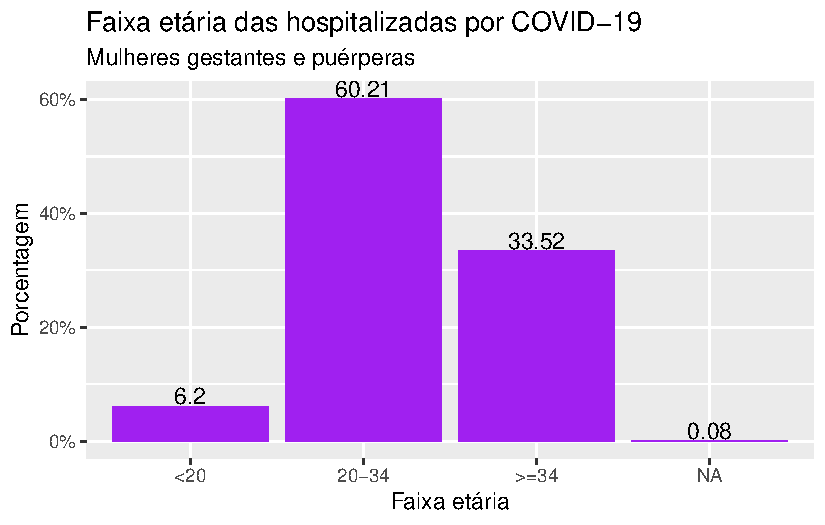
\includegraphics{./descritiva_files/figure-pdf/unnamed-chunk-30-1.pdf}

}

\end{figure}

O argumento \texttt{width} da função \texttt{geom\_bar} permite
controlar a espessura da barra através de valores variando de 0 a 1,
sendo que o tamanho 1 representa o maior tamanho.

\begin{Shaded}
\begin{Highlighting}[]
\FunctionTok{ggplot}\NormalTok{(dados, }\FunctionTok{aes}\NormalTok{(}\AttributeTok{x =}\NormalTok{ faixa\_et, }\AttributeTok{y =}\NormalTok{ (..count..)}\SpecialCharTok{/}\FunctionTok{sum}\NormalTok{(..count..))) }\SpecialCharTok{+}  
  \FunctionTok{geom\_bar}\NormalTok{(}\AttributeTok{fill=}\StringTok{"purple"}\NormalTok{, }\AttributeTok{width=}\FloatTok{0.2}\NormalTok{) }\SpecialCharTok{+} 
  \FunctionTok{geom\_text}\NormalTok{(}\FunctionTok{aes}\NormalTok{(}\AttributeTok{label =} \FunctionTok{round}\NormalTok{((((..count..)}\SpecialCharTok{/}\FunctionTok{sum}\NormalTok{(..count..))}\SpecialCharTok{*}\DecValTok{100}\NormalTok{), }\DecValTok{2}\NormalTok{)), }\AttributeTok{stat=} \StringTok{"count"}\NormalTok{, }\AttributeTok{vjust =} \SpecialCharTok{{-}}\FloatTok{0.1}\NormalTok{)}\SpecialCharTok{+}
  \FunctionTok{scale\_y\_continuous}\NormalTok{(}\AttributeTok{labels=}\NormalTok{scales}\SpecialCharTok{::}\NormalTok{percent) }\SpecialCharTok{+}
  \FunctionTok{labs}\NormalTok{(}\AttributeTok{x =} \StringTok{"Faixa etária"}\NormalTok{, }\AttributeTok{y =} \StringTok{"Porcentagem"}\NormalTok{, }\AttributeTok{title =} \StringTok{"Faixa etária das hospitalizadas por COVID{-}19"}\NormalTok{, }\AttributeTok{subtitle =} \StringTok{"Mulheres gestantes e puérperas"}\NormalTok{)}
\end{Highlighting}
\end{Shaded}

\begin{figure}[H]

{\centering 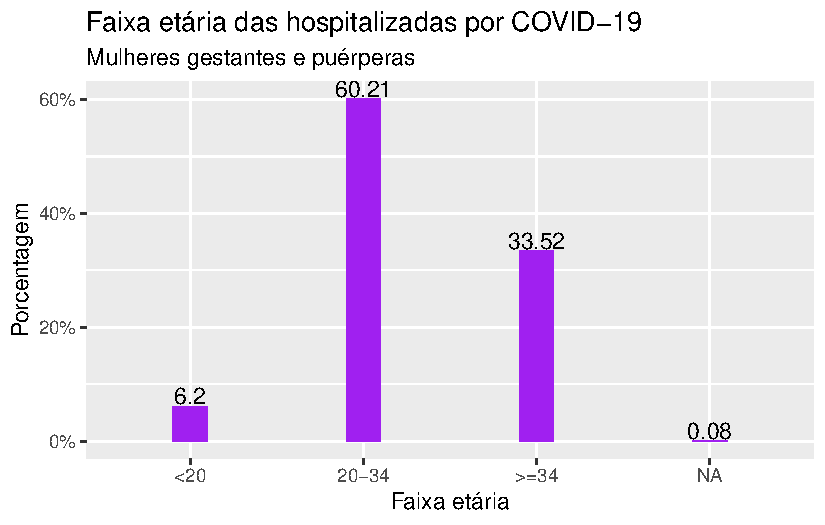
\includegraphics{./descritiva_files/figure-pdf/unnamed-chunk-31-1.pdf}

}

\end{figure}

Para mudar a disposição das barras de vertical para horizontal, basta
acrescentar basta inserir a função \texttt{coord\_flip()}. Para diminuir
o tamanho da letra, ajustamos na função \texttt{geom\_text} alterando os
valores do argumento \texttt{size}.

\begin{Shaded}
\begin{Highlighting}[]
\FunctionTok{ggplot}\NormalTok{(dados, }\FunctionTok{aes}\NormalTok{(}\AttributeTok{x =}\NormalTok{ faixa\_et, }\AttributeTok{y =}\NormalTok{ (..count..)}\SpecialCharTok{/}\FunctionTok{sum}\NormalTok{(..count..))) }\SpecialCharTok{+}  
  \FunctionTok{geom\_bar}\NormalTok{(}\AttributeTok{fill=}\StringTok{"purple"}\NormalTok{) }\SpecialCharTok{+} 
  \FunctionTok{geom\_text}\NormalTok{(}\FunctionTok{aes}\NormalTok{(}\AttributeTok{label =} \FunctionTok{round}\NormalTok{((((..count..)}\SpecialCharTok{/}\FunctionTok{sum}\NormalTok{(..count..))}\SpecialCharTok{*}\DecValTok{100}\NormalTok{), }\DecValTok{2}\NormalTok{)), }\AttributeTok{stat=} \StringTok{"count"}\NormalTok{, }\AttributeTok{hjust =} \DecValTok{0}\NormalTok{, }\AttributeTok{size  =} \DecValTok{3}\NormalTok{) }\SpecialCharTok{+}
  \FunctionTok{scale\_y\_continuous}\NormalTok{(}\AttributeTok{labels=}\NormalTok{scales}\SpecialCharTok{::}\NormalTok{percent) }\SpecialCharTok{+}
  \FunctionTok{labs}\NormalTok{(}\AttributeTok{x =} \StringTok{"Faixa etária"}\NormalTok{, }\AttributeTok{y =} \StringTok{"Porcentagem"}\NormalTok{, }\AttributeTok{title =} \StringTok{"Faixa etária das hospitalizadas por COVID{-}19"}\NormalTok{, }\AttributeTok{subtitle =} \StringTok{"Mulheres gestantes e puérperas"}\NormalTok{)}\SpecialCharTok{+}
  \FunctionTok{coord\_flip}\NormalTok{()}
\end{Highlighting}
\end{Shaded}

\begin{figure}[H]

{\centering 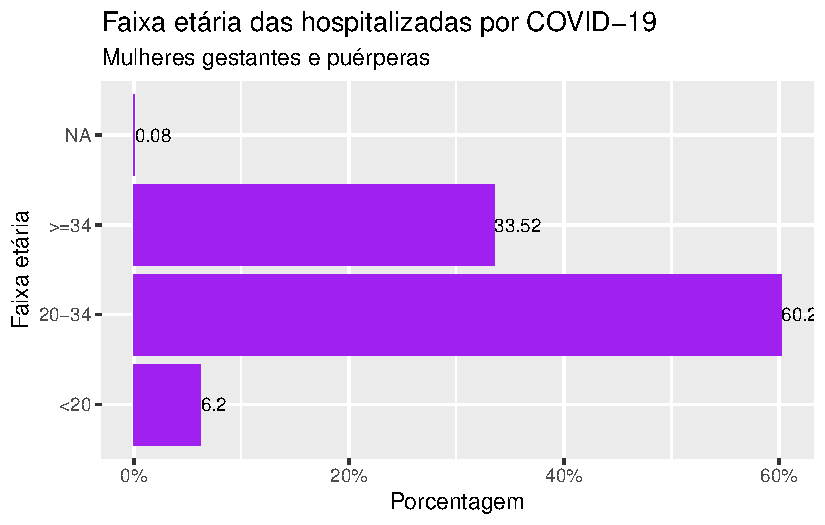
\includegraphics{./descritiva_files/figure-pdf/unnamed-chunk-32-1.pdf}

}

\end{figure}

Vejamos agora como construir um gráfico de barras com duas variáveis
qualitativas conjuntamente. Para exemplificar, vamos considerar as
variáveis faixa etária (\texttt{faixa\_et}) e cardiopatia
(\texttt{cardiopat}). Nosso interesse é analisar a distribuição da
faixa-etária estratificada pelas categorias da variável cardiopatia que,
como vimos antes, podem assumir os resultados ``sim'', ``não'',
``ignorado'' e ``NA''.

\begin{Shaded}
\begin{Highlighting}[]
\FunctionTok{ggplot}\NormalTok{(dados, }\FunctionTok{aes}\NormalTok{(}\AttributeTok{x =}\NormalTok{ faixa\_et, }\AttributeTok{group =}\NormalTok{ cardiopati)) }\SpecialCharTok{+}  
  \FunctionTok{geom\_bar}\NormalTok{(}\FunctionTok{aes}\NormalTok{(}\AttributeTok{y =}\NormalTok{ ..prop..), }\AttributeTok{stat =} \StringTok{"count"}\NormalTok{, }\AttributeTok{fill=}\StringTok{"green4"}\NormalTok{) }\SpecialCharTok{+} 
  \FunctionTok{labs}\NormalTok{(}\AttributeTok{x =} \StringTok{"Faixa etária"}\NormalTok{, }\AttributeTok{y =} \StringTok{"Porcentagem"}\NormalTok{, }\AttributeTok{title =} \StringTok{"Faixa etária das hospitalizadas por COVID{-}19 pela presença de cardiopatia"}\NormalTok{, }\AttributeTok{subtitle =} \StringTok{"Mulheres gestantes e puérperas"}\NormalTok{)}\SpecialCharTok{+}
  \FunctionTok{scale\_y\_continuous}\NormalTok{(}\AttributeTok{labels=}\NormalTok{scales}\SpecialCharTok{::}\NormalTok{percent) }\SpecialCharTok{+}
  \FunctionTok{facet\_grid}\NormalTok{(}\SpecialCharTok{\textasciitilde{}}\NormalTok{cardiopati)}
\end{Highlighting}
\end{Shaded}

\begin{figure}[H]

{\centering 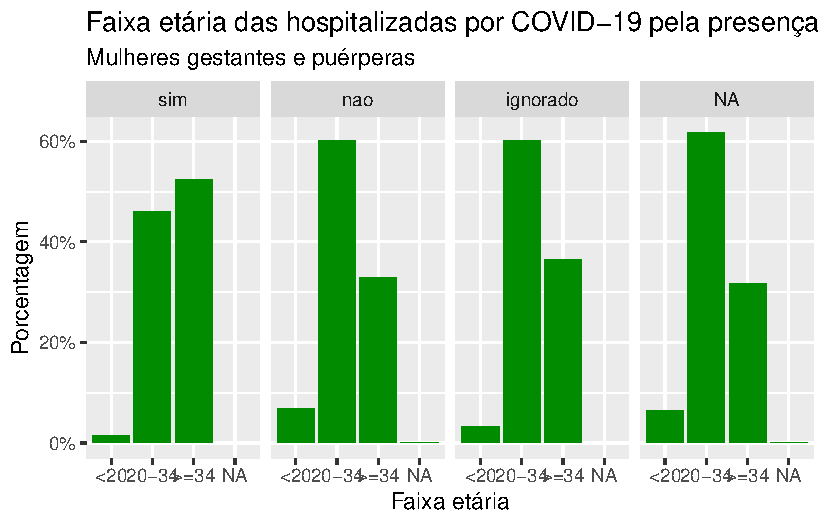
\includegraphics{./descritiva_files/figure-pdf/unnamed-chunk-33-1.pdf}

}

\end{figure}

O próximo código apresenta o gráfico anterior com as porcentagens
inseridas na figura.

\begin{Shaded}
\begin{Highlighting}[]
\FunctionTok{ggplot}\NormalTok{(dados, }\FunctionTok{aes}\NormalTok{(}\AttributeTok{x =}\NormalTok{ faixa\_et, }\AttributeTok{group =}\NormalTok{ cardiopati)) }\SpecialCharTok{+}  
  \FunctionTok{geom\_bar}\NormalTok{(}\FunctionTok{aes}\NormalTok{(}\AttributeTok{y =}\NormalTok{ ..prop..), }\AttributeTok{stat =} \StringTok{"count"}\NormalTok{, }\AttributeTok{fill=}\StringTok{"green4"}\NormalTok{) }\SpecialCharTok{+} 
  \FunctionTok{geom\_text}\NormalTok{(}\FunctionTok{aes}\NormalTok{(}\AttributeTok{label =}\NormalTok{ scales}\SpecialCharTok{::}\FunctionTok{percent}\NormalTok{(..prop.., }\AttributeTok{accuracy =} \FloatTok{0.1}\NormalTok{), }\AttributeTok{y=}\NormalTok{ ..prop..), }\AttributeTok{stat =} \StringTok{"count"}\NormalTok{, }\AttributeTok{vjust =} \SpecialCharTok{{-}}\NormalTok{.}\DecValTok{1}\NormalTok{) }\SpecialCharTok{+}
  \FunctionTok{labs}\NormalTok{(}\AttributeTok{x =} \StringTok{"Faixa etária"}\NormalTok{, }\AttributeTok{y =} \StringTok{"Porcentagem"}\NormalTok{, }\AttributeTok{title =} \StringTok{"Faixa etária das hospitalizadas por COVID{-}19 pela presença de cardiopatia"}\NormalTok{, }\AttributeTok{subtitle =} \StringTok{"Mulheres gestantes e puérperas"}\NormalTok{)}\SpecialCharTok{+}
  \FunctionTok{scale\_y\_continuous}\NormalTok{(}\AttributeTok{labels=}\NormalTok{scales}\SpecialCharTok{::}\NormalTok{percent) }\SpecialCharTok{+}
  \FunctionTok{facet\_grid}\NormalTok{(}\SpecialCharTok{\textasciitilde{}}\NormalTok{cardiopati)}
\end{Highlighting}
\end{Shaded}

\begin{figure}[H]

{\centering 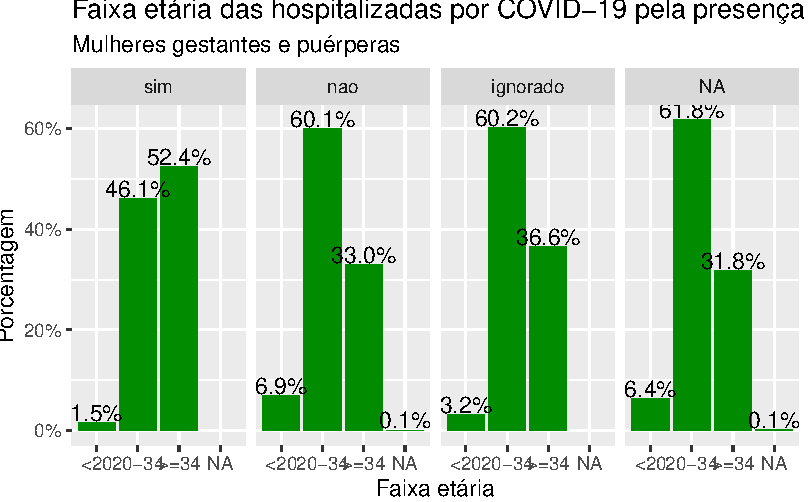
\includegraphics{./descritiva_files/figure-pdf/unnamed-chunk-34-1.pdf}

}

\end{figure}

Vamos agora colocar cada categoria com a sua própria cor, a fim de
facilitar a comparação. Para isso, vamos considerar o argumento
\texttt{fill\ =\ factor(..x..)} na função \texttt{geom\_bar}. Como as
categorias da variável faixa-etária são autoexplicativas, o termo
\texttt{theme(legend.position="none")} for inserido na construção do
gráfico para se evitar a criação de uma nova legenda para as cores
relacionadas as faixas de idade, evitando assim repetição de informação.

\begin{Shaded}
\begin{Highlighting}[]
\FunctionTok{ggplot}\NormalTok{(dados, }\FunctionTok{aes}\NormalTok{(}\AttributeTok{x=}\NormalTok{faixa\_et, }\AttributeTok{group =}\NormalTok{ cardiopati))  }\SpecialCharTok{+} 
  \FunctionTok{geom\_bar}\NormalTok{(}\FunctionTok{aes}\NormalTok{(}\AttributeTok{y =}\NormalTok{ ..prop.., }\AttributeTok{fill =} \FunctionTok{factor}\NormalTok{(..x..)), }\AttributeTok{stat=}\StringTok{"count"}\NormalTok{) }\SpecialCharTok{+}
  \FunctionTok{geom\_text}\NormalTok{(}\FunctionTok{aes}\NormalTok{(}\AttributeTok{label =}\NormalTok{ scales}\SpecialCharTok{::}\FunctionTok{percent}\NormalTok{(..prop.., }\AttributeTok{accuracy =} \FloatTok{0.1}\NormalTok{), }\AttributeTok{y=}\NormalTok{ ..prop..), }\AttributeTok{stat=} \StringTok{"count"}\NormalTok{, }\AttributeTok{vjust =} \SpecialCharTok{{-}}\NormalTok{.}\DecValTok{1}\NormalTok{) }\SpecialCharTok{+}
  \FunctionTok{labs}\NormalTok{(}\AttributeTok{x =} \StringTok{"Faixa etária"}\NormalTok{, }\AttributeTok{y =} \StringTok{"Porcentagem"}\NormalTok{, }\AttributeTok{title =} \StringTok{"Faixa etária das hospitalizadas por COVID{-}19 pela presença de cardiopatia"}\NormalTok{, }\AttributeTok{subtitle =} \StringTok{"Mulheres gestantes e puérperas"}\NormalTok{)}\SpecialCharTok{+}
  \FunctionTok{theme}\NormalTok{(}\AttributeTok{legend.position=}\StringTok{"none"}\NormalTok{)}\SpecialCharTok{+}
  \FunctionTok{scale\_y\_continuous}\NormalTok{(}\AttributeTok{labels=}\NormalTok{scales}\SpecialCharTok{::}\NormalTok{percent) }\SpecialCharTok{+}
  \FunctionTok{facet\_grid}\NormalTok{(}\SpecialCharTok{\textasciitilde{}}\NormalTok{cardiopati)}
\end{Highlighting}
\end{Shaded}

\begin{figure}[H]

{\centering 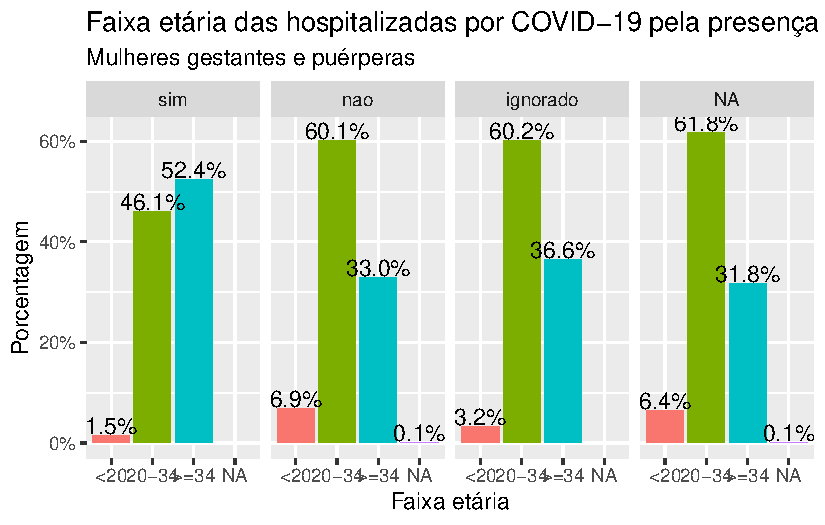
\includegraphics{./descritiva_files/figure-pdf/unnamed-chunk-35-1.pdf}

}

\end{figure}

A escala de cores utilizada por padrão pela função \texttt{geom\_bar}
nem sempre atende a todos os públicos. O pacote \texttt{viridis} do R
apresenta escalas de cores projetadas para melhorar a legibilidade dos
gráficos para leitores com formas comuns de daltonismo e/ou deficiência
em visão de cores. Para usá-lo, devemos inserir a função
\texttt{scale\_fill\_manual(values\ =\ c(viridis(4)))}, com o valor 4
representando as 4 categorias da faixa etária.

\begin{Shaded}
\begin{Highlighting}[]
\FunctionTok{library}\NormalTok{(viridis)}

\FunctionTok{ggplot}\NormalTok{(dados, }\FunctionTok{aes}\NormalTok{(}\AttributeTok{x=}\NormalTok{faixa\_et, }\AttributeTok{group =}\NormalTok{ cardiopati))  }\SpecialCharTok{+} 
  \FunctionTok{geom\_bar}\NormalTok{(}\FunctionTok{aes}\NormalTok{(}\AttributeTok{y =}\NormalTok{ ..prop.., }\AttributeTok{fill =} \FunctionTok{factor}\NormalTok{(..x..)), }\AttributeTok{stat=}\StringTok{"count"}\NormalTok{) }\SpecialCharTok{+}
  \FunctionTok{geom\_text}\NormalTok{(}\FunctionTok{aes}\NormalTok{(}\AttributeTok{label =}\NormalTok{ scales}\SpecialCharTok{::}\FunctionTok{percent}\NormalTok{(..prop.., }\AttributeTok{accuracy =} \FloatTok{0.1}\NormalTok{), }\AttributeTok{y=}\NormalTok{ ..prop..), }\AttributeTok{stat=} \StringTok{"count"}\NormalTok{, }\AttributeTok{vjust =} \SpecialCharTok{{-}}\NormalTok{.}\DecValTok{1}\NormalTok{) }\SpecialCharTok{+}
  \FunctionTok{labs}\NormalTok{(}\AttributeTok{x =} \StringTok{"Faixa etária"}\NormalTok{, }\AttributeTok{y =} \StringTok{"Porcentagem"}\NormalTok{, }\AttributeTok{title =} \StringTok{"Faixa etária das hospitalizadas por COVID{-}19 pela presença de cardiopatia"}\NormalTok{, }\AttributeTok{subtitle =} \StringTok{"Mulheres gestantes e puérperas"}\NormalTok{)}\SpecialCharTok{+}
  \FunctionTok{theme}\NormalTok{(}\AttributeTok{legend.position=}\StringTok{"none"}\NormalTok{)}\SpecialCharTok{+}
  \FunctionTok{scale\_y\_continuous}\NormalTok{(}\AttributeTok{labels=}\NormalTok{scales}\SpecialCharTok{::}\NormalTok{percent) }\SpecialCharTok{+}
  \FunctionTok{scale\_fill\_manual}\NormalTok{(}\AttributeTok{values =} \FunctionTok{c}\NormalTok{(}\FunctionTok{viridis}\NormalTok{(}\DecValTok{4}\NormalTok{))) }\SpecialCharTok{+}
  \FunctionTok{facet\_grid}\NormalTok{(}\SpecialCharTok{\textasciitilde{}}\NormalTok{cardiopati)}
\end{Highlighting}
\end{Shaded}

\begin{figure}[H]

{\centering 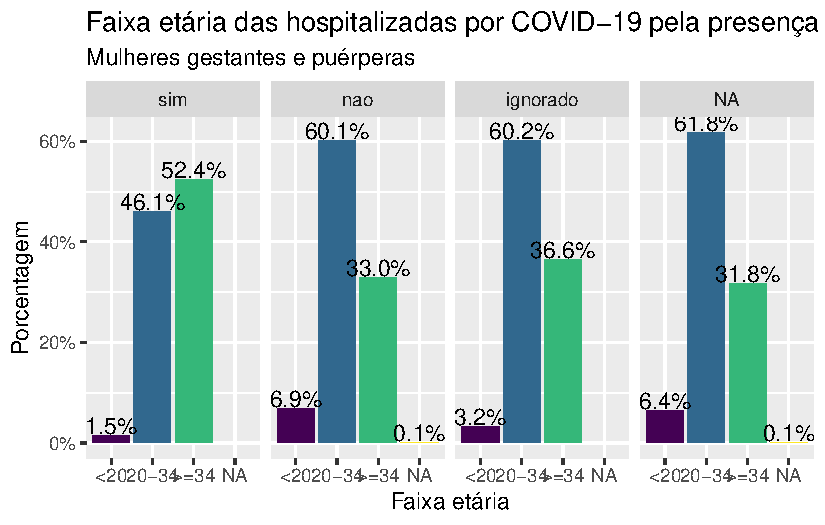
\includegraphics{./descritiva_files/figure-pdf/unnamed-chunk-36-1.pdf}

}

\end{figure}

Vários dos gráficos aqui mencionados podem construídos fazendo usos de
outras funções e código do pacote do \texttt{ggplot2}. Especificamente
sobre o gráfico de barras, na página
(http://www.sthda.com/english/wiki/ggplot2-barplots-quick-start-guide-r-software-and-data-visualization\#barplot-of-counts)
podemos encontrar outras interessantes customizações gráficas que podem
ser implementadas via pacote \texttt{ggplot2}.

\hypertarget{gruxe1ficos-para-variuxe1veis-quantitativas}{%
\subsubsection{Gráficos para variáveis
quantitativas}\label{gruxe1ficos-para-variuxe1veis-quantitativas}}

Todos os códigos apresentados anteriormente podem ser usados quando a
variável de interesse é quantitativa discreta com poucos valores
diferentes. No caso de haver muitos diferentes valores para a variável
quantitativa discreta, gráficos do tipo histograma costumam ser mais
informativos. Vamos apresentar agora ferramentas para a construção de
gráficos para esse tipo de variável e para variáveis quantitativas
contínuas. Todos os gráficos a serem construídos daqui para frente farão
uso da paleta \texttt{viridis}. Vejamos a construção do histograma de
densidades para a variável \texttt{idade}.

A função considerada agora é \texttt{geom\_histogram}. O argumento
\texttt{y\ =\ ..density..} indica que queremos apresentar o histograma
de densidades, \texttt{bins\ =\ 15} refere-se ao número de barras
contíguas que queremos que o gráfico apresente, ´fill´ designa a cor a
preencher o gráfico e color é a cor da linha das barras.

\begin{Shaded}
\begin{Highlighting}[]
\FunctionTok{ggplot}\NormalTok{(dados, }\FunctionTok{aes}\NormalTok{(}\AttributeTok{x=}\NormalTok{idade))  }\SpecialCharTok{+} 
  \FunctionTok{geom\_histogram}\NormalTok{(}\FunctionTok{aes}\NormalTok{(}\AttributeTok{y =}\NormalTok{ ..density..), }\AttributeTok{bins =} \DecValTok{15}\NormalTok{, }\AttributeTok{fill =} \FunctionTok{viridis}\NormalTok{(}\DecValTok{1}\NormalTok{), }\AttributeTok{color =} \StringTok{"black"}\NormalTok{) }\SpecialCharTok{+}
  \FunctionTok{labs}\NormalTok{(}\AttributeTok{x =} \StringTok{"Idade"}\NormalTok{, }\AttributeTok{y =} \StringTok{"Densidade"}\NormalTok{, }\AttributeTok{title =} \StringTok{"Histograma de densidades das idades de hospitalizadas por COVID{-}19"}\NormalTok{, }\AttributeTok{subtitle =} \StringTok{"Mulheres gestantes e puérperas"}\NormalTok{)}
\end{Highlighting}
\end{Shaded}

\begin{figure}[H]

{\centering 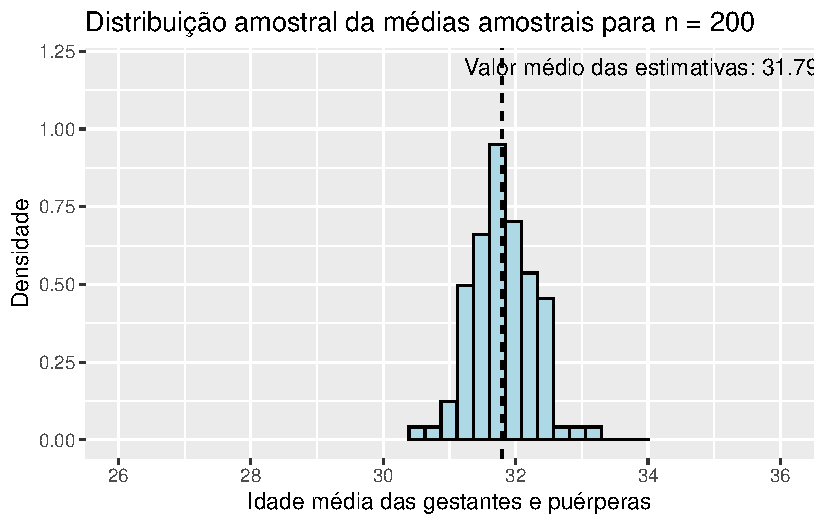
\includegraphics{./descritiva_files/figure-pdf/unnamed-chunk-37-1.pdf}

}

\end{figure}

Enquanto medida, densidade corresponde a razão entre o número de casos
contabilizados em intervalo e a amplitude do intervalo. Uma das
vantagens em considerar o histograma de densidades e não o histograma de
frequências é que a área total sob o gráfico corresponde a 1, deixando o
gráfico na mesma escala de funções de densidade. Por exemplo, na figura
a seguir inserimos uma versão alisada empírica do histograma. O
argumento \texttt{alpha} na função \texttt{geom\_density} controla o
nível de transparência das cores preenchidas no histograma alisado e
varia de 0 a 1, com 1 representando a cor sólida.

\begin{Shaded}
\begin{Highlighting}[]
\FunctionTok{ggplot}\NormalTok{(dados, }\FunctionTok{aes}\NormalTok{(}\AttributeTok{x=}\NormalTok{idade))  }\SpecialCharTok{+} 
  \FunctionTok{geom\_histogram}\NormalTok{(}\FunctionTok{aes}\NormalTok{(}\AttributeTok{y =}\NormalTok{ ..density..), }\AttributeTok{bins =} \DecValTok{15}\NormalTok{, }\AttributeTok{fill =} \FunctionTok{viridis}\NormalTok{(}\DecValTok{1}\NormalTok{), }\AttributeTok{color =} \StringTok{"black"}\NormalTok{) }\SpecialCharTok{+}
  \FunctionTok{geom\_density}\NormalTok{(}\AttributeTok{fill =} \StringTok{"grey55"}\NormalTok{, }\AttributeTok{color =} \StringTok{"grey80"}\NormalTok{, }\AttributeTok{alpha =} \FloatTok{0.2}\NormalTok{) }\SpecialCharTok{+}
  \FunctionTok{labs}\NormalTok{(}\AttributeTok{x =} \StringTok{"Idade"}\NormalTok{, }\AttributeTok{y =} \StringTok{"Densidade"}\NormalTok{, }\AttributeTok{title =} \StringTok{"Histograma de densidades das idades de hospitalizadas por COVID{-}19 "}\NormalTok{, }\AttributeTok{subtitle =} \StringTok{"Mulheres gestantes e puérperas"}\NormalTok{)}
\end{Highlighting}
\end{Shaded}

\begin{figure}[H]

{\centering 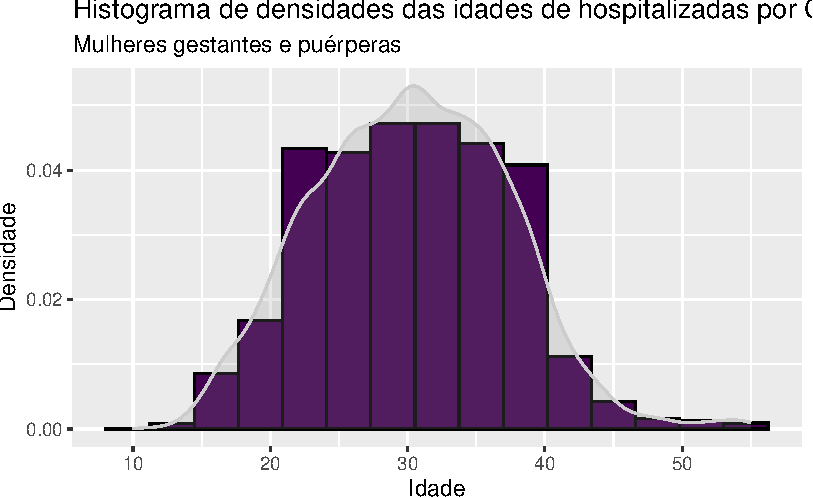
\includegraphics{./descritiva_files/figure-pdf/unnamed-chunk-38-1.pdf}

}

\end{figure}

No código a seguir apresentamos uma maneira de construir o histograma de
densidades de uma variável quantitativa nas diferentes categorias de uma
variável qualitativa. Aqui a variável qualitativa refere-se a
informações sobre o \(status\) de cardiopatia e a variável quantitativa
considerada foi a idade. Para facilitar a comparação das diferentes
faixas de valores da variável quantitativa entre as categorias, vamos
inserir uma escala inserir uma escala de cores entre as faixas de
valores, deixando o gráfico com um aspecto bastante atrativo e
informativo. O argumento considerado na função \texttt{geom\_density} é
\texttt{fill\ =\ ..x..}, informando que o preenchimento do histograma
será realizado nas faixas de valores da variável quantitativa. Para a
escala de cores, inserimos a função
\texttt{scale\_fill\_gradientn(colours\ =\ c(viridis(15)))}, em que o
valor 15 corresponde ao número de barras contíguas
(\texttt{bins\ =\ 15}) considerado no histograma.

\begin{Shaded}
\begin{Highlighting}[]
\FunctionTok{ggplot}\NormalTok{(dados, }\FunctionTok{aes}\NormalTok{(}\AttributeTok{x=}\NormalTok{idade))  }\SpecialCharTok{+} 
  \FunctionTok{geom\_histogram}\NormalTok{(}\FunctionTok{aes}\NormalTok{(}\AttributeTok{y =}\NormalTok{ ..density.., }\AttributeTok{fill=}\NormalTok{..x..), }\AttributeTok{bins =} \DecValTok{15}\NormalTok{, }\AttributeTok{color =} \StringTok{"black"}\NormalTok{) }\SpecialCharTok{+}
  \FunctionTok{geom\_density}\NormalTok{(}\AttributeTok{fill =} \StringTok{"grey55"}\NormalTok{, }\AttributeTok{color =} \StringTok{"grey80"}\NormalTok{, }\AttributeTok{alpha =} \FloatTok{0.2}\NormalTok{) }\SpecialCharTok{+}
  \FunctionTok{labs}\NormalTok{(}\AttributeTok{x =} \StringTok{"Idade"}\NormalTok{, }\AttributeTok{y =} \StringTok{"Densidade"}\NormalTok{, }\AttributeTok{title =} \StringTok{"Histogramas de densidades das idades fixado status de cardiopatia "}\NormalTok{, }\AttributeTok{subtitle =} \StringTok{"Gestantes e puérperas hospitalizadas por COVID{-}19"}\NormalTok{)}\SpecialCharTok{+}
  \FunctionTok{scale\_fill\_gradientn}\NormalTok{(}\AttributeTok{colours =} \FunctionTok{c}\NormalTok{(}\FunctionTok{viridis}\NormalTok{(}\DecValTok{15}\NormalTok{)))}\SpecialCharTok{+}
  \FunctionTok{theme}\NormalTok{(}\AttributeTok{legend.position=}\StringTok{"none"}\NormalTok{)}\SpecialCharTok{+}
  \FunctionTok{facet\_grid}\NormalTok{(}\SpecialCharTok{\textasciitilde{}}\NormalTok{cardiopati)}
\end{Highlighting}
\end{Shaded}

\begin{figure}[H]

{\centering 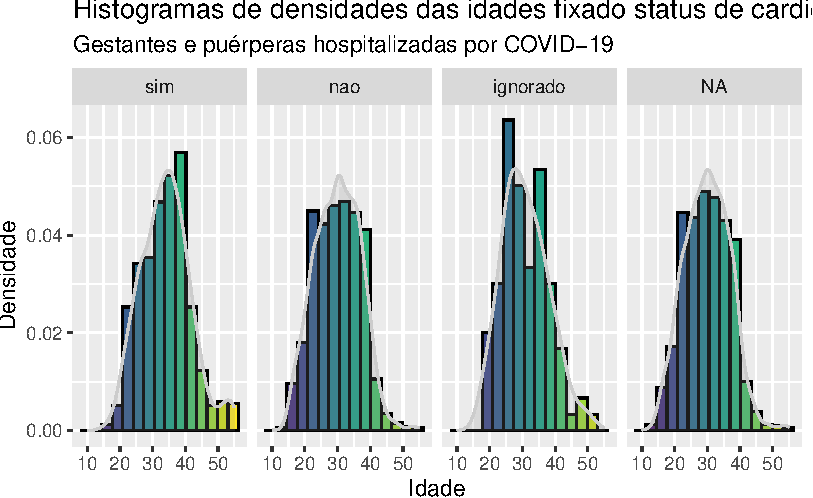
\includegraphics{./descritiva_files/figure-pdf/unnamed-chunk-39-1.pdf}

}

\end{figure}

Para que os histogramas sejam dispostos um abaixo do outro, basta
substituir a função \texttt{facet\_grid(\textasciitilde{}cardiopati)}
por \texttt{facet\_wrap(\textasciitilde{}cardiopati,\ ncol=1)}.

\begin{Shaded}
\begin{Highlighting}[]
\FunctionTok{ggplot}\NormalTok{(dados, }\FunctionTok{aes}\NormalTok{(}\AttributeTok{x=}\NormalTok{idade))  }\SpecialCharTok{+} 
  \FunctionTok{geom\_histogram}\NormalTok{(}\FunctionTok{aes}\NormalTok{(}\AttributeTok{y =}\NormalTok{ ..density.., }\AttributeTok{fill=}\NormalTok{..x..), }\AttributeTok{bins =} \DecValTok{15}\NormalTok{, }\AttributeTok{color =} \StringTok{"black"}\NormalTok{) }\SpecialCharTok{+}
  \FunctionTok{geom\_density}\NormalTok{(}\AttributeTok{fill =} \StringTok{"grey55"}\NormalTok{, }\AttributeTok{color =} \StringTok{"grey80"}\NormalTok{, }\AttributeTok{alpha =} \FloatTok{0.2}\NormalTok{) }\SpecialCharTok{+}
  \FunctionTok{labs}\NormalTok{(}\AttributeTok{x =} \StringTok{"Idade"}\NormalTok{, }\AttributeTok{y =} \StringTok{"Densidade"}\NormalTok{, }\AttributeTok{title =} \StringTok{"Histogramas de densidades das idades fixado status de cardiopatia "}\NormalTok{, }\AttributeTok{subtitle =} \StringTok{"Gestantes e puérperas hospitalizadas por COVID{-}19"}\NormalTok{)}\SpecialCharTok{+}
  \FunctionTok{scale\_fill\_gradientn}\NormalTok{(}\AttributeTok{colours =} \FunctionTok{c}\NormalTok{(}\FunctionTok{viridis}\NormalTok{(}\DecValTok{15}\NormalTok{)))}\SpecialCharTok{+}
  \FunctionTok{theme}\NormalTok{(}\AttributeTok{legend.position=}\StringTok{"none"}\NormalTok{)}\SpecialCharTok{+}
  \FunctionTok{facet\_wrap}\NormalTok{(}\SpecialCharTok{\textasciitilde{}}\NormalTok{cardiopati, }\AttributeTok{ncol=}\DecValTok{1}\NormalTok{)}
\end{Highlighting}
\end{Shaded}

\begin{figure}[H]

{\centering 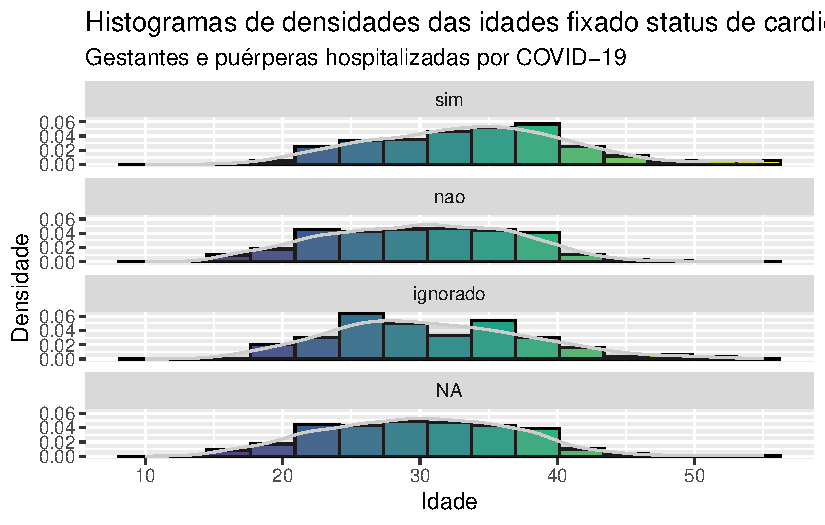
\includegraphics{./descritiva_files/figure-pdf/unnamed-chunk-40-1.pdf}

}

\end{figure}

Caso se queira apresentar os histogramas alisados sobrepostos por
categoria, pode-se usar o código proposto na sequência.

\begin{Shaded}
\begin{Highlighting}[]
\FunctionTok{ggplot}\NormalTok{(dados, }\FunctionTok{aes}\NormalTok{(}\AttributeTok{x =}\NormalTok{ idade, }\AttributeTok{fill =}\NormalTok{ cardiopati)) }\SpecialCharTok{+}
  \FunctionTok{geom\_density}\NormalTok{(}\AttributeTok{alpha =} \FloatTok{0.5}\NormalTok{) }\SpecialCharTok{+}
  \FunctionTok{labs}\NormalTok{(}\AttributeTok{x =} \StringTok{"Idade"}\NormalTok{, }\AttributeTok{y =} \StringTok{"Densidade"}\NormalTok{, }\AttributeTok{title =} \StringTok{"Histogramas alisados das idades pelo status de cardiopatia"}\NormalTok{, }\AttributeTok{subtitle =} \StringTok{"Gestantes e puérperas hospitalizadas por COVID{-}19"}\NormalTok{) }\SpecialCharTok{+}
  \FunctionTok{scale\_fill\_manual}\NormalTok{(}\AttributeTok{values =} \FunctionTok{c}\NormalTok{(}\FunctionTok{viridis}\NormalTok{(}\DecValTok{3}\NormalTok{)), }\AttributeTok{name =} \StringTok{"Cardiopatia"}\NormalTok{)}
\end{Highlighting}
\end{Shaded}

\begin{figure}[H]

{\centering 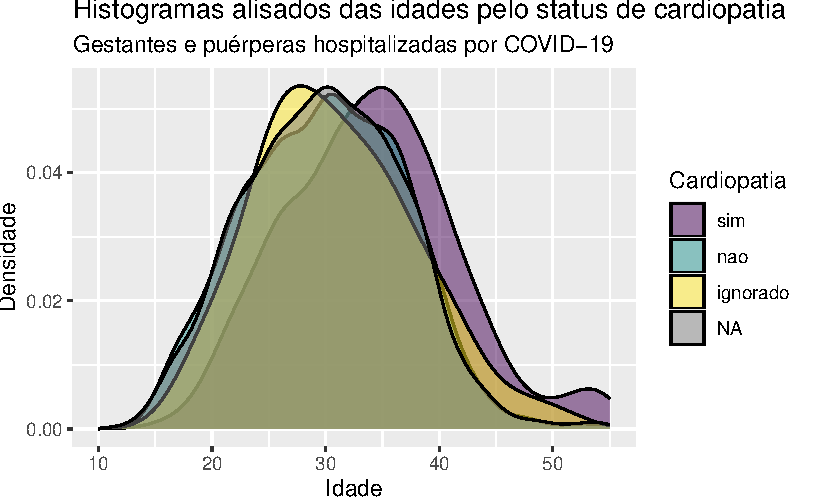
\includegraphics{./descritiva_files/figure-pdf/unnamed-chunk-41-1.pdf}

}

\end{figure}

Um outro gráfico muito utilizado na apresentação de uma variável
quantitativa é o boxplot que apresenta, visualmente, os valores mínimo,
primeiro quartil (Q1), mediana ou segundo quartil (Q2), terceiro quartil
(Q3), máximo e possíveis \(outliers\). Baseado nessas medidas, temos uma
ideia do comportamento da variável quantitativa em termos de posição,
dispersão, assimetria e dados discrepantes. A posição central é dada
pela mediana e a dispersão pelo intervalo interquartil. As posições
relativas entre Q1, Q2 e Q3 nos dão uma ideia da simetria ou assimetria
da distribuição.

\begin{figure}

{\centering 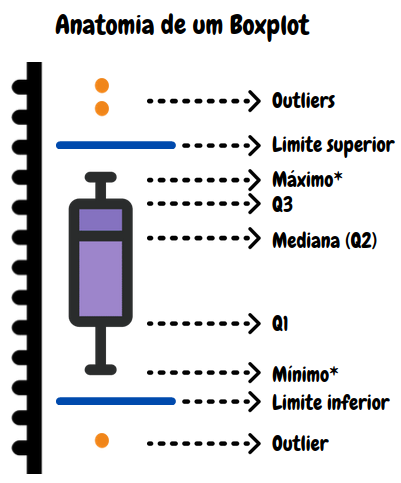
\includegraphics{./figuras_descritiva/Boxplot2.png}

}

\end{figure}

Os valores \(Q_1\), \(Q_2\) e \(Q_3\) já foram apresentados
anteriormente. No gráfico, o segundo quartil (ou seja, a mediana) é
representada pela linha que corta a caixa do boxplot. Já o primeiro
quartil (\(Q_1\)) é a base da caixa e o terceiro quartil (\(Q_3\)), o
topo. O intervalo interquartil está representado na altura da caixa. A
escolha do tamanho da base da caixa é arbitrária, devendo-se tão somente
garantir que as linhas \(Q_1\), \(Q_2\) e \(Q3\) estão localizadas na
altura em que os valores dos quartis foram obtidos.

As linhas em azul são linhas imaginárias (normalmente não aparecem
graficadas nos gráficos) e representam valores que distinguem valores
\(outliers\) dos demais. Valores \(outliers\) são valores considerados
discrepantes dentro do conjunto de dados de uma variável. Para a
representação no boxplot, são considerados \(outliers\), observações com
valores maiores que o Limite Superior (LS) ou com valores menores que o
Limite Inferior (LI), tal que \(LI = Q_1 - 1.5 (Q_3 - Q_1)\) e
\(LS = Q_3 + 1.5 (Q_3 - Q_1)\). Ainda na figura, observamos a presença
de um \(\mbox{Mínimo}^*\) e \(\mbox{Máximo}^*\) que nem sempre
representam o menor e a maior, respectivamente, observações na amostra.
Por definição, \(\mbox{Mínimo}^*\) é o menor valor maior que o Limite
Inferior (LI), ou seja, é o menor valor observado no conjunto de dados
desconsiderado os valores \(outliers\). Analogamente,
\(\mbox{Máximo}^*\) é o maior valor menor que o Limite Superior (LS), ou
seja, é o maior valor observado no conjunto de dados desconsiderado os
valores \(outliers\).

No pacote \texttt{ggplot2}, esse gráfico é construído com a função
\texttt{geom\_boxplot} que apresenta argumentos similares aos gráficos
de barras e histograma.

\begin{Shaded}
\begin{Highlighting}[]
\FunctionTok{ggplot}\NormalTok{(dados, }\FunctionTok{aes}\NormalTok{(}\AttributeTok{y=}\NormalTok{idade))  }\SpecialCharTok{+} 
  \FunctionTok{geom\_boxplot}\NormalTok{(}\AttributeTok{fill =} \FunctionTok{viridis}\NormalTok{(}\DecValTok{1}\NormalTok{), }\AttributeTok{color =} \StringTok{"black"}\NormalTok{) }\SpecialCharTok{+}
  \FunctionTok{labs}\NormalTok{(}\AttributeTok{x =} \StringTok{""}\NormalTok{, }\AttributeTok{y =} \StringTok{"Idade"}\NormalTok{, }\AttributeTok{title =} \StringTok{"Boxplot das idades de hospitalizadas por COVID{-}19 "}\NormalTok{, }\AttributeTok{subtitle =} \StringTok{"Mulheres gestantes e puérperas"}\NormalTok{)}
\end{Highlighting}
\end{Shaded}

\begin{figure}[H]

{\centering 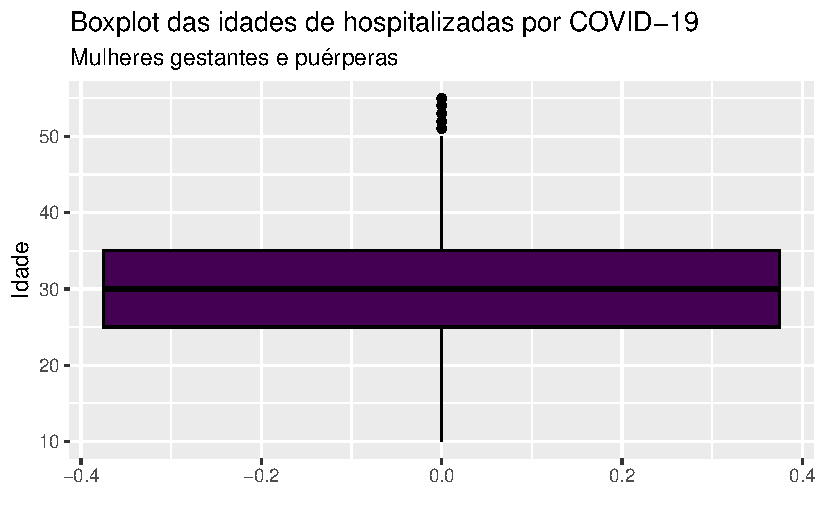
\includegraphics{./descritiva_files/figure-pdf/unnamed-chunk-42-1.pdf}

}

\end{figure}

O boxplot, assim como o histograma, também pode ser utilizado para
apresentar o comportamento de variáveis quantitativas em função das
categorias de variáveis qualitativas.

\begin{Shaded}
\begin{Highlighting}[]
\FunctionTok{ggplot}\NormalTok{(dados, }\FunctionTok{aes}\NormalTok{(}\AttributeTok{y=}\NormalTok{idade, }\AttributeTok{x =}\NormalTok{ cardiopati))  }\SpecialCharTok{+} 
  \FunctionTok{geom\_boxplot}\NormalTok{(}\AttributeTok{fill =} \FunctionTok{viridis}\NormalTok{(}\DecValTok{1}\NormalTok{), }\AttributeTok{color =} \StringTok{"black"}\NormalTok{) }\SpecialCharTok{+}
  \FunctionTok{labs}\NormalTok{(}\AttributeTok{x =} \StringTok{""}\NormalTok{, }\AttributeTok{y =} \StringTok{"Idade"}\NormalTok{, }\AttributeTok{title =} \StringTok{"Boxplot das idades fixado status de cardiopatia"}\NormalTok{, }\AttributeTok{subtitle =} \StringTok{"Gestantes e puérperas hospitalizadas por COVID{-}19"}\NormalTok{)}
\end{Highlighting}
\end{Shaded}

\begin{figure}[H]

{\centering 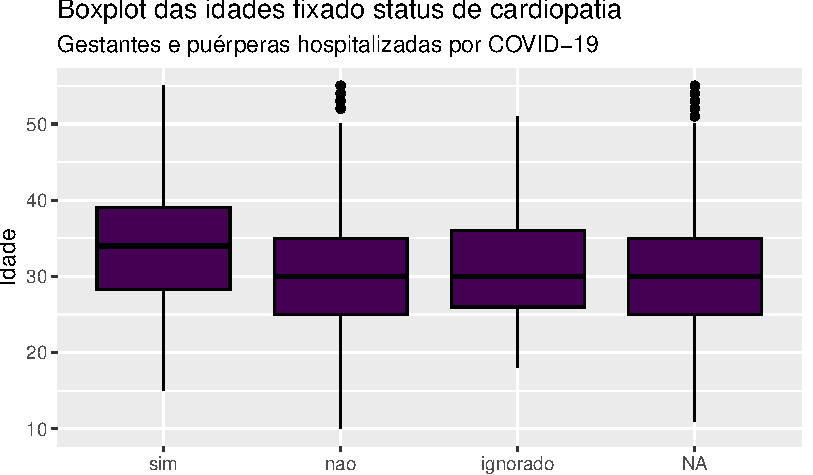
\includegraphics{./descritiva_files/figure-pdf/unnamed-chunk-43-1.pdf}

}

\end{figure}

Para que cada categoria apresente sua própria cor, basta declarar qual a
variável que será considerada para colorir os boxplots em suas
categorias via argumento \texttt{fill} em \texttt{ggplot} e indicar
quais as cores serão utilizadas. Como a variável cardiopatia
(\texttt{cardiopati}) tem 4 categorias, informamos as cores na função
\texttt{geom\_boxplot} usando o termo \texttt{fill\ =\ viridis(4)}. Além
disso, caso se tenha interesse em destacar as observações \(outliers\)
com outras cores, pode ser usado o argumento \texttt{outlier.color} na
função \texttt{geom\_boxplot}. Por exemplo, na figura abaixo, vamos
destacar os \(outliers\) em vermelho.

\begin{Shaded}
\begin{Highlighting}[]
\FunctionTok{ggplot}\NormalTok{(dados, }\FunctionTok{aes}\NormalTok{(}\AttributeTok{y=}\NormalTok{idade, }\AttributeTok{x =}\NormalTok{ cardiopati, }\AttributeTok{fill =}\NormalTok{ cardiopati))  }\SpecialCharTok{+} 
  \FunctionTok{geom\_boxplot}\NormalTok{(}\AttributeTok{fill =} \FunctionTok{viridis}\NormalTok{(}\DecValTok{4}\NormalTok{), }\AttributeTok{color =} \StringTok{"black"}\NormalTok{, }\AttributeTok{outlier.color =} \StringTok{"red"}\NormalTok{) }\SpecialCharTok{+}
  \FunctionTok{labs}\NormalTok{(}\AttributeTok{x =} \StringTok{""}\NormalTok{, }\AttributeTok{y =} \StringTok{"Idade"}\NormalTok{, }\AttributeTok{title =} \StringTok{"Boxplot das idades fixado status de cardiopatia"}\NormalTok{, }\AttributeTok{subtitle =} \StringTok{"Gestantes e puérperas hospitalizadas por COVID{-}19"}\NormalTok{)}
\end{Highlighting}
\end{Shaded}

\begin{figure}[H]

{\centering 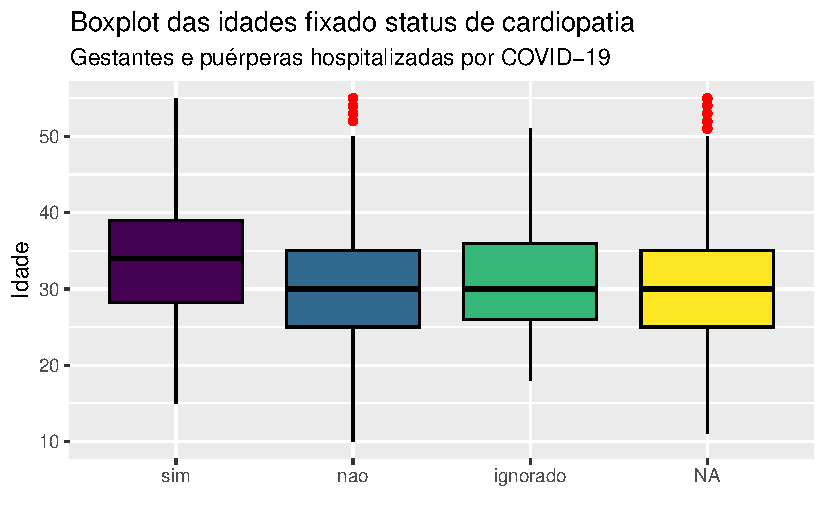
\includegraphics{./descritiva_files/figure-pdf/unnamed-chunk-44-1.pdf}

}

\end{figure}

No código a seguir, vamos apresentar o boxplot da variável quantitativa
idade pela variável qualitativa \(status\) de cardiopatia, estratificado
nas diferentes categorias de evolução do caso. Para clareza do texto no
gráfico, a legenda da variável cardiopatia foi colocada abaixo dele,
assim como o texto no eixo horizontal foi disposto de forma inclinada,
através da função
\texttt{theme(legend.position="bottom",\ axis.text.x=element\_text(angle=30,\ hjust=0.8))}.

\begin{Shaded}
\begin{Highlighting}[]
\FunctionTok{ggplot}\NormalTok{(dados, }\FunctionTok{aes}\NormalTok{(}\AttributeTok{y=}\NormalTok{idade, }\AttributeTok{x =}\NormalTok{ cardiopati, }\AttributeTok{fill =}\NormalTok{ cardiopati))  }\SpecialCharTok{+} 
  \FunctionTok{geom\_boxplot}\NormalTok{(}\AttributeTok{color =} \StringTok{"black"}\NormalTok{) }\SpecialCharTok{+}
  \FunctionTok{labs}\NormalTok{(}\AttributeTok{x =} \StringTok{""}\NormalTok{, }\AttributeTok{y =} \StringTok{"Idade"}\NormalTok{, }\AttributeTok{title =} \StringTok{"Boxplot das idades pelo status de cardiopatia, fixada a evolução"}\NormalTok{, }\AttributeTok{subtitle =} \StringTok{"Gestantes e puérperas hospitalizadas por COVID{-}19"}\NormalTok{)}\SpecialCharTok{+}
  \FunctionTok{theme}\NormalTok{(}\AttributeTok{legend.position=}\StringTok{"bottom"}\NormalTok{, }\AttributeTok{axis.text.x=}\FunctionTok{element\_text}\NormalTok{(}\AttributeTok{angle=}\DecValTok{30}\NormalTok{, }\AttributeTok{hjust=}\FloatTok{0.8}\NormalTok{)) }\SpecialCharTok{+}
  \FunctionTok{scale\_fill\_manual}\NormalTok{(}\AttributeTok{values =} \FunctionTok{c}\NormalTok{(}\FunctionTok{viridis}\NormalTok{(}\DecValTok{4}\NormalTok{)), }\AttributeTok{name =} \StringTok{"Cardiopatia"}\NormalTok{)}\SpecialCharTok{+}
  \FunctionTok{facet\_grid}\NormalTok{(}\SpecialCharTok{\textasciitilde{}}\NormalTok{evolucao)}
\end{Highlighting}
\end{Shaded}

\begin{figure}[H]

{\centering 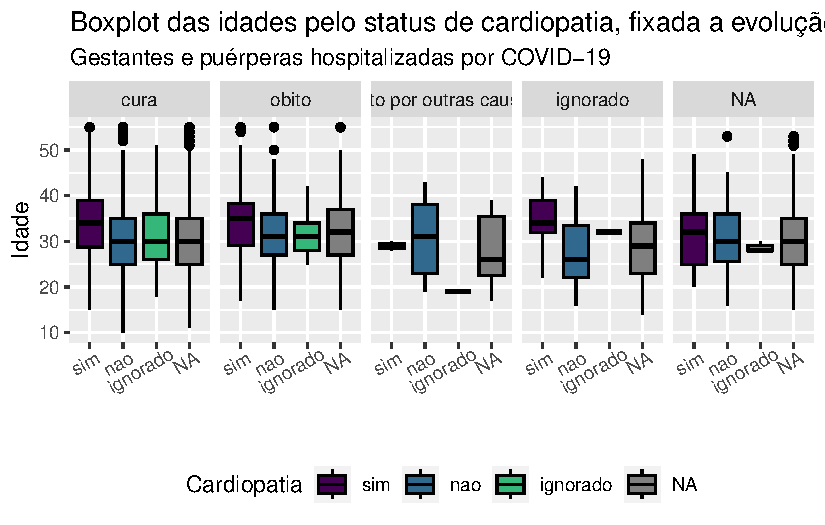
\includegraphics{./descritiva_files/figure-pdf/unnamed-chunk-45-1.pdf}

}

\end{figure}

Nosso objetivo agora é explorar a construção de gráficos quando temos
duas variáveis quantitativas através do diagrama de dispersão. Para
exemplificar a construção, vamos considerar as variáveis do banco de
dados \texttt{dados\_uti\_res} que contém as variáveis idade e
quantidade de dias em uti (\texttt{dias\_uti}).

\begin{Shaded}
\begin{Highlighting}[]
\FunctionTok{ggplot}\NormalTok{(dados\_uti\_res, }\FunctionTok{aes}\NormalTok{(}\AttributeTok{x=}\NormalTok{idade, }\AttributeTok{y =}\NormalTok{ dias\_uti))  }\SpecialCharTok{+} 
  \FunctionTok{geom\_point}\NormalTok{(}\AttributeTok{colour =} \FunctionTok{viridis}\NormalTok{(}\DecValTok{1}\NormalTok{)) }\SpecialCharTok{+}
  \FunctionTok{labs}\NormalTok{(}\AttributeTok{x =} \StringTok{"Idade"}\NormalTok{, }\AttributeTok{y =} \StringTok{"Dias em UTI "}\NormalTok{, }\AttributeTok{title =} \StringTok{"Gráfico de dispersão da idade pelo tempo em UTI"}\NormalTok{, }\AttributeTok{subtitle =} \StringTok{"Gestantes e puérperas hospitalizadas por COVID{-}19"}\NormalTok{)}
\end{Highlighting}
\end{Shaded}

\begin{figure}[H]

{\centering 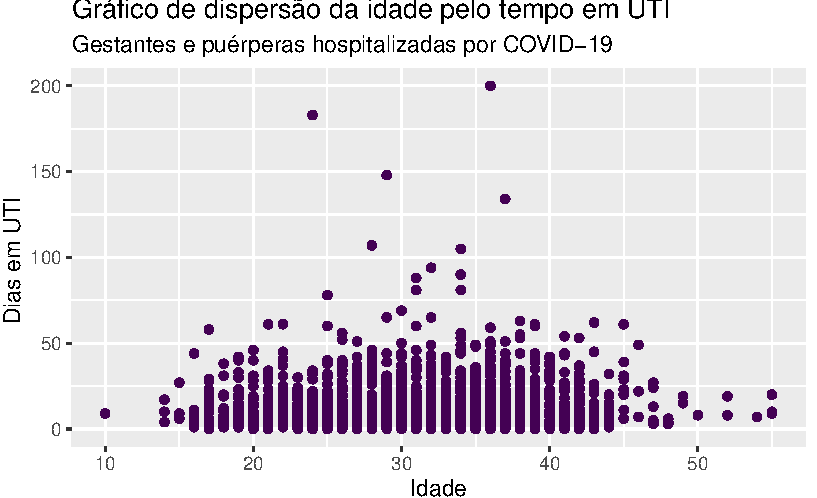
\includegraphics{./descritiva_files/figure-pdf/unnamed-chunk-46-1.pdf}

}

\end{figure}

O pacote \texttt{ggExtra} consegue inserir no gráfico de dispersão
gerado pelo \texttt{ggplot2} histogramas, histogramas alisados e boxplot
das variáveis marginais. Para isso, basta utilizar a função
\texttt{ggMarginal} informando o nome do objeto em que está guardado o
gráfico de dispersão e o tipo de gráfico marginal a ser inserido.

\begin{Shaded}
\begin{Highlighting}[]
\NormalTok{p }\OtherTok{\textless{}{-}} \FunctionTok{ggplot}\NormalTok{(dados\_uti\_res, }\FunctionTok{aes}\NormalTok{(}\AttributeTok{x=}\NormalTok{idade, }\AttributeTok{y =}\NormalTok{ dias\_uti))  }\SpecialCharTok{+} 
  \FunctionTok{geom\_point}\NormalTok{(}\AttributeTok{colour =} \FunctionTok{viridis}\NormalTok{(}\DecValTok{1}\NormalTok{)) }\SpecialCharTok{+}
  \FunctionTok{labs}\NormalTok{(}\AttributeTok{x =} \StringTok{"Idade"}\NormalTok{, }\AttributeTok{y =} \StringTok{"Dias em UTI "}\NormalTok{, }\AttributeTok{title =} \StringTok{"Gráfico de dispersão da idade pelo tempo em UTI"}\NormalTok{, }\AttributeTok{subtitle =} \StringTok{"Gestantes e puérperas hospitalizadas por COVID{-}19"}\NormalTok{)}

\FunctionTok{library}\NormalTok{(ggExtra)}

\CommentTok{\# histograma marginal}
\FunctionTok{ggMarginal}\NormalTok{(p, }\AttributeTok{type=}\StringTok{"histogram"}\NormalTok{)}
\end{Highlighting}
\end{Shaded}

\begin{figure}[H]

{\centering 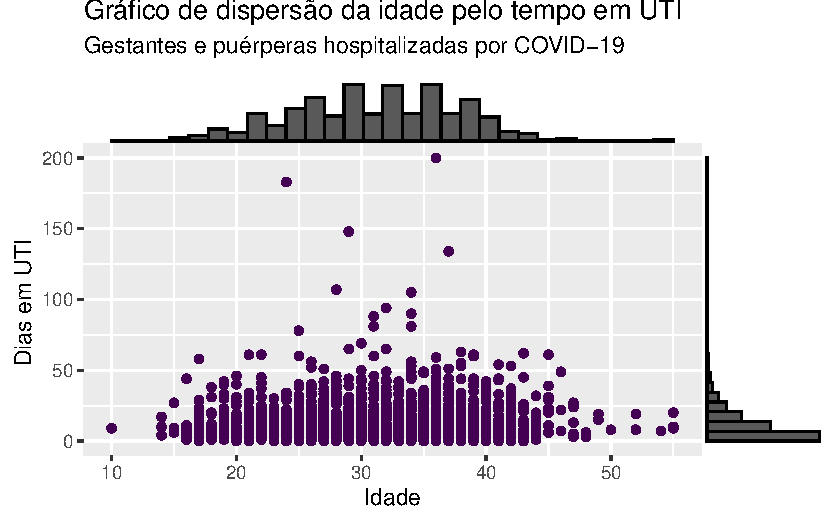
\includegraphics{./descritiva_files/figure-pdf/unnamed-chunk-47-1.pdf}

}

\end{figure}

\begin{Shaded}
\begin{Highlighting}[]
\CommentTok{\# histograma alisado marginal}
\FunctionTok{ggMarginal}\NormalTok{(p, }\AttributeTok{type=}\StringTok{"density"}\NormalTok{)}
\end{Highlighting}
\end{Shaded}

\begin{figure}[H]

{\centering 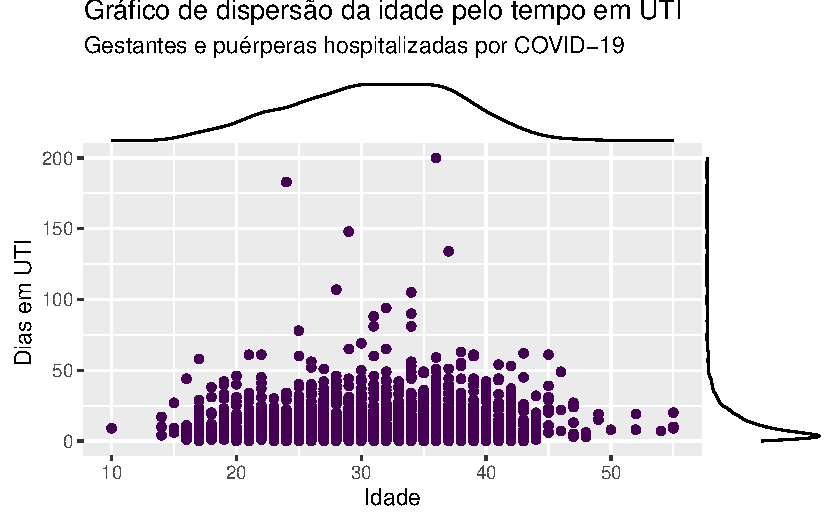
\includegraphics{./descritiva_files/figure-pdf/unnamed-chunk-48-1.pdf}

}

\end{figure}

\begin{Shaded}
\begin{Highlighting}[]
\CommentTok{\# Boxplot marginal}
\FunctionTok{ggMarginal}\NormalTok{(p, }\AttributeTok{type=}\StringTok{"boxplot"}\NormalTok{)}
\end{Highlighting}
\end{Shaded}

\begin{figure}[H]

{\centering 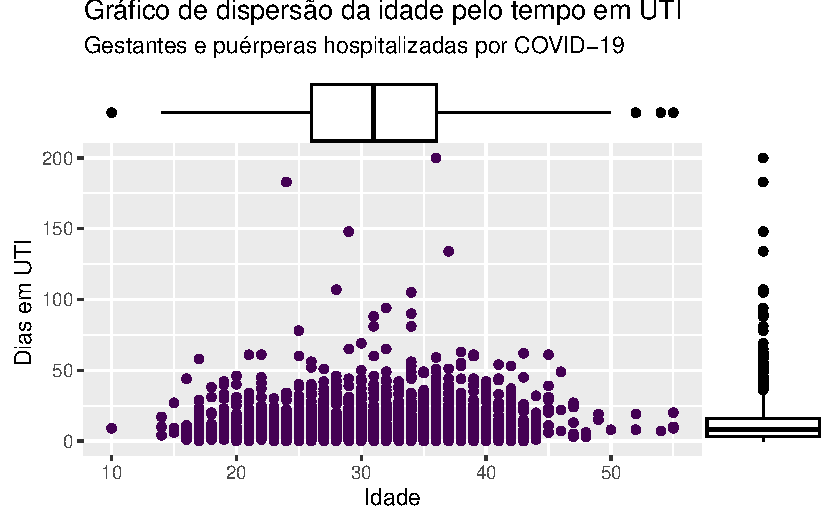
\includegraphics{./descritiva_files/figure-pdf/unnamed-chunk-49-1.pdf}

}

\end{figure}

Podemos construir gráficos de dispersão estratificados por categorias de
uma variável qualitativa. No código abaixo, vamos utilizar o \(status\)
de cardiopatia e, para isso, usamos o argumento
\texttt{color\ =\ cardiopati} na função \texttt{geom\_point}.

\begin{Shaded}
\begin{Highlighting}[]
\FunctionTok{ggplot}\NormalTok{(dados\_uti\_res, }\FunctionTok{aes}\NormalTok{(}\AttributeTok{x=}\NormalTok{idade, }\AttributeTok{y =}\NormalTok{ dias\_uti))  }\SpecialCharTok{+} 
  \FunctionTok{geom\_point}\NormalTok{(}\FunctionTok{aes}\NormalTok{(}\AttributeTok{color =}\NormalTok{ cardiopati)) }\SpecialCharTok{+}
  \FunctionTok{scale\_colour\_viridis\_d}\NormalTok{(}\StringTok{"Cardiopatia"}\NormalTok{, }\AttributeTok{na.value =} \StringTok{"grey50"}\NormalTok{)}\SpecialCharTok{+}
  \FunctionTok{labs}\NormalTok{(}\AttributeTok{x =} \StringTok{"Idade"}\NormalTok{, }\AttributeTok{y =} \StringTok{"Dias em UTI "}\NormalTok{, }\AttributeTok{title =} \StringTok{"Gráfico de dispersão da idade pelo tempo em UTI, fixado status de cardiopatia"}\NormalTok{, }\AttributeTok{subtitle =} \StringTok{"Gestantes e puérperas hospitalizadas por COVID{-}19"}\NormalTok{)}
\end{Highlighting}
\end{Shaded}

\begin{figure}[H]

{\centering 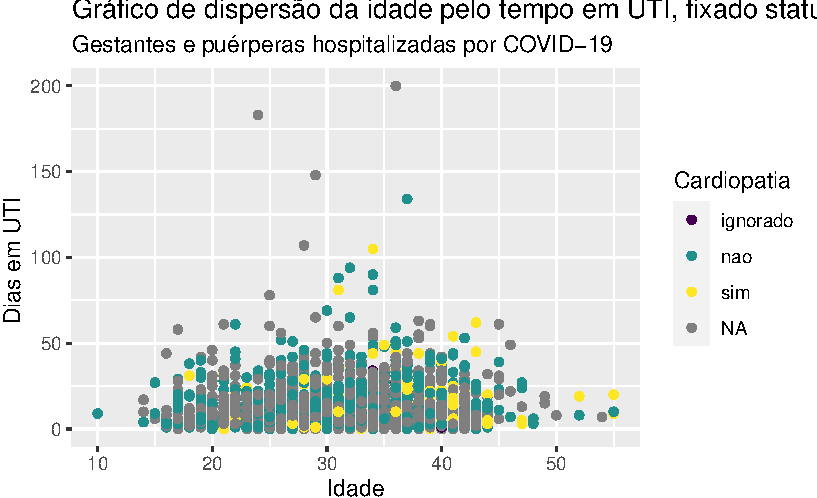
\includegraphics{./descritiva_files/figure-pdf/unnamed-chunk-50-1.pdf}

}

\end{figure}

Como pontos de diferentes cores estão sobrepondo, uma visualização
possível para facilitar a análise pode ser feita separando os diagramas
de dispersão em diferentes planos cartesianos de mesma escala.

\begin{Shaded}
\begin{Highlighting}[]
\FunctionTok{ggplot}\NormalTok{(dados\_uti\_res, }\FunctionTok{aes}\NormalTok{(}\AttributeTok{x=}\NormalTok{idade, }\AttributeTok{y =}\NormalTok{ dias\_uti))  }\SpecialCharTok{+} 
  \FunctionTok{geom\_point}\NormalTok{(}\FunctionTok{aes}\NormalTok{(}\AttributeTok{color =}\NormalTok{ cardiopati)) }\SpecialCharTok{+}
  \FunctionTok{scale\_colour\_viridis\_d}\NormalTok{(}\StringTok{"Cardiopatia"}\NormalTok{, }\AttributeTok{na.value =} \StringTok{"grey50"}\NormalTok{)}\SpecialCharTok{+}
  \FunctionTok{labs}\NormalTok{(}\AttributeTok{x =} \StringTok{"Idade"}\NormalTok{, }\AttributeTok{y =} \StringTok{"Dias em UTI "}\NormalTok{, }\AttributeTok{title =} \StringTok{"Gráfico de dispersão da idade pelo tempo em UTI, fixado status de cardiopatia"}\NormalTok{, }\AttributeTok{subtitle =} \StringTok{"Gestantes e puérperas hospitalizadas por COVID{-}19"}\NormalTok{)}\SpecialCharTok{+}
  \FunctionTok{facet\_wrap}\NormalTok{(}\SpecialCharTok{\textasciitilde{}}\NormalTok{cardiopati, }\AttributeTok{ncol=}\DecValTok{1}\NormalTok{)}
\end{Highlighting}
\end{Shaded}

\begin{figure}[H]

{\centering 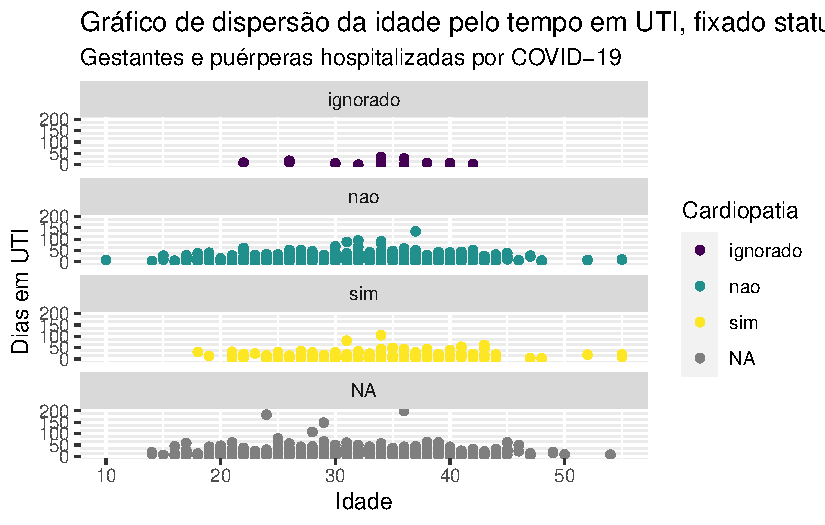
\includegraphics{./descritiva_files/figure-pdf/unnamed-chunk-51-1.pdf}

}

\end{figure}

\hypertarget{pacote-esquisse}{%
\subsection{Pacote esquisse}\label{pacote-esquisse}}

O pacote \texttt{esquisse} disponibiliza um \(dashboard\) interativo
para criação de gráficos por meio do pacote \texttt{ggplot2}.

\begin{Shaded}
\begin{Highlighting}[]
\FunctionTok{library}\NormalTok{(esquisse)}
\end{Highlighting}
\end{Shaded}

Ao rodar a função \texttt{esquisser()}, um janela é aberta (veja
Figura~\ref{fig-Eq1}), em que usuário deve escolher a base de dados a
trabalhar. Feito isso, uma outra janela será aberta apresentando todas
as variáveis presentes no banco de dados escolhido (veja
Figura~\ref{fig-Eq2}), permitindo assim fazer os gráficos. Preparamos um
tutorial para a utilização do pacote \texttt{esquisse} que pode ser
acessado aqui {(https://www.youtube.com/watch?XXXXXXXXXXXXX)} .

\begin{figure}

{\centering 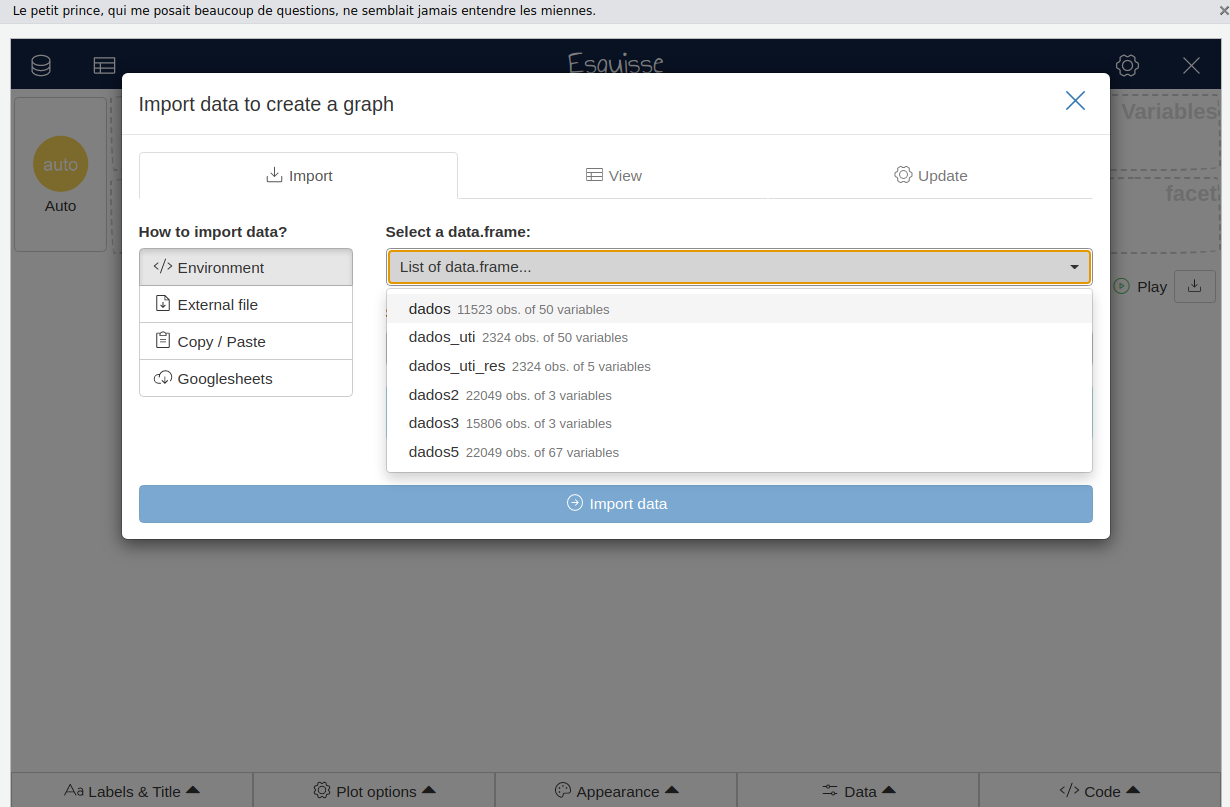
\includegraphics{./figuras_descritiva/Esquisser_1.png}

}

\caption{\label{fig-Eq1}Primeira tela do esquisser.}

\end{figure}

\begin{figure}

{\centering 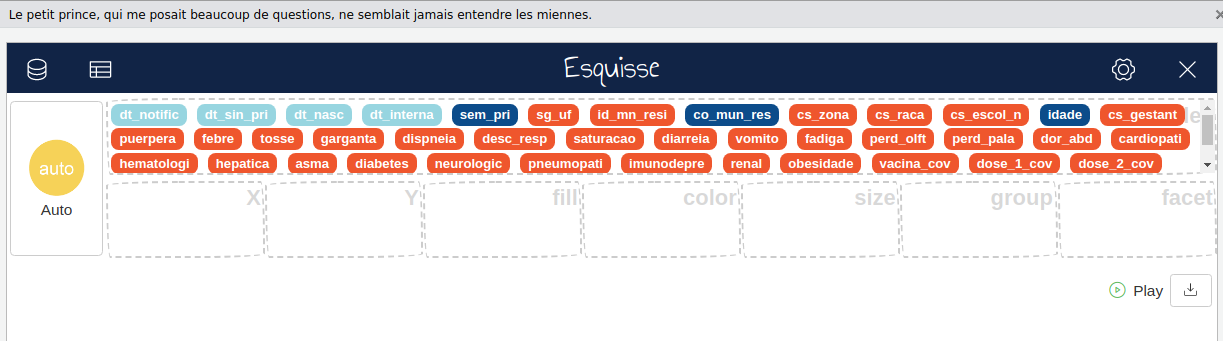
\includegraphics{./figuras_descritiva/Esquisser_2.png}

}

\caption{\label{fig-Eq2}Segunda tela do esquisser.}

\end{figure}

\hypertarget{materiais-complementares}{%
\subsection{Materiais complementares}\label{materiais-complementares}}

Livros e Artigos:

\begin{itemize}
\item
  Mercier F, Consalvo N, Frey N, Phipps A, Ribba B. From waterfall plots
  to spaghetti plots in early oncology clinical development. Pharm Stat.
  2019;18(5):526-532. doi:10.1002/pst.1944
\item
  Gillespie TW. Understanding waterfall plots. J Adv Pract Oncol.
  2012;3(2):106-111.
\item
  Sonnad SS. Describing data: statistical and graphical methods.
  Radiology. 2002;225(3):622-628. doi:10.1148/radiol.2253012154
\item
  In J, Lee S. Statistical data presentation. Korean J Anesthesiol.
  2017;70(3):267-276. doi:10.4097/kjae.2017.70.3.267
\item
  Morettin P, Singer J. Estatística e Ciência de Dados. 1nd ed.~LTC;
  2022.
\end{itemize}

\(Sites\):

\begin{itemize}
\tightlist
\item
  https://r-graph-gallery.com/index.html\\
\item
  http://www.sthda.com/english/wiki/data-visualization
\item
  https://www.cedricscherer.com/2019/08/05/a-ggplot2-tutorial-for-beautiful-plotting-in-r/
\end{itemize}

\bookmarksetup{startatroot}

\hypertarget{estimauxe7uxe3o}{%
\chapter{Estimação}\label{estimauxe7uxe3o}}

Neste capítulo, iniciando no mundo da Inferência Estatística, trataremos
sobre o problema da \textbf{estimação}. É muito comum, no dia a dia, nos
depararmos com situações em que temos interesse no valor de uma
quantidade desconhecida a respeito de alguma população que estamos
estudando. Utilizando os dados sobre a COVID-19 apresentados
anteriormente, suponha, por exemplo, que tivéssemos interesse na idade
média das gestantes e puérperas hospitalizadas por COVID-19 e que vieram
a óbito por conta dessa doença no período de março de 2020 a dezembro de
2021, ou que nossa intenção fosse investigar a proporção de doentes que
apresentaram diarreia como um de seus sintomas nesse mesmo período. A
essas quantidades da população, que em geral são desconhecidas, damos,
na Estatística, o nome de \textbf{parâmetro}.

Apesar de, no presente caso, termos acesso aos dados de toda a população
de gestantes e puérperas hospitalizadas pela COVID-19 no período
especificado, conhecer o verdadeiro valor de um parâmetro é, na maior
parte das vezes, uma tarefa impraticável, seja pela extensão da
população, pelo tempo que seria gasto para se realizar tal estudo ou
mesmo pela falta de recursos disponíveis. Com isso, acabamos tendo de
recorrer à coleta de uma \textbf{amostra}, uma pequena porção do todo
que nos permita estudar as quantidades que temos interesse. Uma amostra
representativa da população nos permite obter boas \emph{estimativas}
para os valores dos parâmetros que estamos investigando, e a aplicação
de métodos inferenciais nos possibilita estender, à população, as
conclusões que fizemos para a amostra obtida. Quando as estimativas se
dão apenas por um único valor, as chamamos de \textbf{estimativas
pontuais}. Por outro lado, quando as estimativas são formadas por um
intervalo de valores plausíveis para o parâmetro, as chamamos de
\textbf{estimativas intervalares}. Discutiremos sobre ambos os tipos de
estimativas ao longo deste capítulo. Antes, entretanto, precisamos
entender alguns conceitos básicos de probabilidade e inferência para que
a viagem ao longo desse novo universo não seja tão turbulenta.

\hypertarget{conceitos-buxe1sicos-de-probabilidade}{%
\section{Conceitos básicos de
probabilidade}\label{conceitos-buxe1sicos-de-probabilidade}}

A fazer

\hypertarget{estimadores-e-estimativas}{%
\section{Estimadores e estimativas}\label{estimadores-e-estimativas}}

Agora que estamos a parte de algumas definições que serão importantes
para o entendimento do capítulo, podemos iniciar com o seu conteúdo
propriamente dito. Em primeiro lugar, chamamos de \textbf{estimador}
qualquer estatística cujos valores são utilizados para se estimar um
parâmetro ou uma função de um parâmetro. Dessa forma, temos, portanto,
que todo estimador será, também, uma variável aleatória, uma vez que
eles são funções das variáveis aleatórias que compõem nossa amostra.
Quando coletamos a amostra, observamos os valores das variáveis
aleatórias que a compõem e os substituímos na expressão do estimador,
obtemos o que chamamos de \textbf{estimativa}. Estimativas não são
valores aleatórios, mas sim realizações de variáveis aleatórias (dos
estimadores).

Diversos métodos foram desenvolvidos ao longo dos anos para se encontrar
estatísticas que possam ser utilizadas como estimadores. Entre os mais
conhecidos, podemos citar: o \textbf{método dos momentos}, que encontra
estimadores relacionando os \textbf{momentos} amostrais e populacionais;
o \textbf{método dos mínimos quadrados}, a partir do qual encontramos o
estimador que minimiza a chamada \textbf{soma de quadrado dos erros}; e
o \textbf{método da máxima verossimilhança}, provavelmente o mais
conhecido e utilizado, por meio do qual encontramos o estimador que
maximiza a probabilidade de a amostra coletada ter sido observada,
através da maximização da \textbf{função de verossimilhança}. Não
entraremos em maiores detalhes sobre nenhum desses métodos, uma vez que
nosso objetivo aqui é introduzir o conceito de estimação de forma mais
intuitiva. Entretanto, caso seja de seu interesse, já publicamos, no
site do Observatório, um texto que pode te ajudar a entender o método da
máxima verossimilhança e tudo aquilo que está por trás dele. O post está
disponível neste link .

O problema da estimação não se resume somente a encontrar estimadores.
De fato, existem infinitos estimadores para qualquer que seja o
parâmetro que tenhamos interesse. A questão agora é, então, estabelecer
critérios que nos permitam determinar o melhor estimador em um certo
conjunto. Nesse contexto, podemos definir uma série de propriedades que
os estimadores possuem ou podem possuir. São elas:

\begin{itemize}
\item
  \textbf{Vício:} dizemos que um estimador é \textbf{não viciado} (ou
  não viesado) se o seu valor esperado coincide com o verdadeiro valor
  do parâmetro em questão. Em outras palavras, estimadores não viciados
  acertam, em média, o valor do parâmetro que estão estimando. Caso essa
  afirmação não seja verdadeira, dizemos que o estimador apresenta
  \textbf{vício}. O vício é a diferença entre o verdadeiro valor do
  parâmetro e o valor esperado de seu estimador.
\item
  \textbf{Consistência:} dizemos que um estimador é \textbf{consistente}
  se, à medida que o tamanho da amostra aumenta, o seu valor esperado
  converge para o verdadeiro valor do parâmetro em questão e sua
  variância converge para zero. Dessa forma, estimadores consistentes
  não necessariamente são não viciados para tamanhos pequenos de
  amostra: eles só precisam ser não viciados quando esse tamanho é muito
  grande.
\item
  \textbf{Erro quadrático médio:} definimos o erro quadrático médio como
  sendo o valor esperado da diferença quadrática entre o estimador e o
  verdadeiro valor do parâmetro estimado. Tal como a variância de uma
  variável aleatória é uma medida da dispersão de seus valores em torno
  de sua média, o erro quadrático médio é uma medida da dispersão dos
  valores do estimador em torno do verdadeiro valor do parâmetro. Dessa
  forma, estimadores com erros quadráticos médios pequenos são
  preferíveis. Algo a se notar é que o erro quadrático médio pode ser
  reescrito como sendo a soma entre o quadrado do vício do estimador e
  sua variância. Com isso, para estimadores não viciados, o erro
  quadrático médio se reduz à variância do estimador.
\end{itemize}

Em um mundo ideal, parece ser intuitivo que nossa busca pelo melhor
estimador se dê através do erro quadrático médio, tentando encontrar
aquele para o qual essa medida seja a menor possível. Essa tarefa é,
entretanto, raramente possível. Em geral, o erro quadrático médio de um
estimador é uma função do valor desconhecido do parâmetro a ser
estimado, e é muito comum que, para dois estimadores de um parâmetro,
seus erros quadráticos médios se entrelassem: para certos valores do
parâmetro, o primeiro estimador pode ter o menor erro quadrático médio,
enquanto para outros valores o segundo estimador é o que o tem. Com
isso, em nossa busca pelo melhor estimador, é comum restringirmos o
conjunto de todos os estimadores possíveis à classe dos estimadores não
viciados, fazendo com que o erro quadrático médio seja apenas uma função
da variância do estimador. Essa restrição é feita porque existem
técnicas que nos permitem encontrar, entre os estimadores não viciados,
aqueles que possuem a menor variância possível. Não trataremos dessas
técnicas ao longo deste livro, mas essa é uma importante consideração
para se entender o motivo de, em geral, trabalharmos com estimadores não
viciados. De toda forma, passemos, então, para a próxima seção, na qual
veremos alguns exemplos de estimadores pontuais utilizando os dados
apresentados e tratados em capítulos anteriores.

\hypertarget{estimauxe7uxe3o-pontual}{%
\section{Estimação pontual}\label{estimauxe7uxe3o-pontual}}

Para iniciar esta seção, comecemos com uma definição. Chamamos de
\textbf{estimação pontual} a técnica de estimação na qual utilizamos um
único valor de uma estatística para representarmos, ou estimarmos, o
valor desconhecido de um parâmetro de interesse. Chamamos essa
estatística de \textbf{estimador pontual}, enquanto ao seu valor
observado damos o nome de \textbf{estimativa pontual}. {[}completar{]}

\hypertarget{estimauxe7uxe3o-pontual-da-muxe9dia-de-uma-populauxe7uxe3o}{%
\subsection{Estimação pontual da média de uma
população}\label{estimauxe7uxe3o-pontual-da-muxe9dia-de-uma-populauxe7uxe3o}}

Voltando aos exemplos apresentados na introdução do capítulo, suponha,
primeiramente, que nosso parâmetro de interesse seja a idade média das
gestantes e puérperas hospitalizadas por COVID-19 que vieram a óbito por
conta dessa doença no período de março de 2020 a dezembro de 2021, a
qual denotaremos por \(\mu\). Como temos acesso a todos os registros
dessa população, o valor desse parâmetro não é desconhecido, mas isso
servirá de auxílio para exemplificar os métodos que aqui serão
empregados. Criando um vetor contendo todos os elementos da população,
temos:

\begin{Shaded}
\begin{Highlighting}[]
\NormalTok{dados }\OtherTok{\textless{}{-}}\NormalTok{ readr}\SpecialCharTok{::}\FunctionTok{read\_rds}\NormalTok{(}\StringTok{"dados/dados\_covid[LIMPO].rds"}\NormalTok{)}
\NormalTok{populacao1 }\OtherTok{\textless{}{-}}\NormalTok{ dados}\SpecialCharTok{$}\NormalTok{idade\_anos[}\FunctionTok{which}\NormalTok{(dados}\SpecialCharTok{$}\NormalTok{evolucao }\SpecialCharTok{==} \StringTok{"óbito"}\NormalTok{)]}
\FunctionTok{length}\NormalTok{(populacao1)}
\end{Highlighting}
\end{Shaded}

\begin{verbatim}
[1] 1266
\end{verbatim}

O processo envolvido na criação do vetor \texttt{populacao1} é o
seguinte: dentro do data frame \texttt{dados}, que contém todos os
registros de nossa população, estamos selecionando o valor da variável
\texttt{idade\_anos} de todas as pacientes para as quais o valor da
variável \texttt{evolucao} é ``óbito''. O tamanho desse vetor, obtido
por meio da função \texttt{length()}, do pacote básico
\texttt{\{base\}}, é de 1266. Ou seja, a população de gestantes e
puérperas hospitalizadas por COVID-19 que vieram a óbito por conta dessa
doença no período considerado é composta por 1266 elementos. Para
calcular o valor da idade média dessas mulheres, podemos utilizar a
função \texttt{mean()}, também do pacote básico \texttt{\{base\}}, que
calcula a média aritmética de um dado vetor.

\begin{Shaded}
\begin{Highlighting}[]
\FunctionTok{mean}\NormalTok{(populacao1)}
\end{Highlighting}
\end{Shaded}

\begin{verbatim}
[1] 31.80806
\end{verbatim}

A saída do código nos revela o valor de \(31.81\) anos. Note que esse
valor não representa uma estimativa; ele é, de fato, o verdadeiro valor
do parâmetro \(\mu\). O que aconteceria, entretanto, se tivéssemos
acesso apenas a uma amostra da população em questão? Poderíamos garantir
que os resultados obtidos seriam válidos para todas as gestantes e
puérperas desse grupo? É o que começaremos a ver na subseção seguinte.

\hypertarget{trabalhando-com-amostras-da-populauxe7uxe3o}{%
\subsubsection{Trabalhando com amostras da
população}\label{trabalhando-com-amostras-da-populauxe7uxe3o}}

Para exemplificar os conceitos de estimação definidos anteriormente,
simularemos a retirada de amostras da população de gestantes e puérperas
com a qual estamos trabalhando. Dentre as várias maneiras de se obter
amostras de uma população, utilizaremos, aqui, a \textbf{amostragem
aleatória simples (AAS) com reposição}, uma técnica de amostragem
probabilística (ou seja, que atribui a cada elemento da população uma
probabilidade, conhecida \emph{a priori}, de pertencer à amostra), na
qual todos os elementos da população possuem a mesma probabilidade de
serem sorteados. Utilizaremos a AAS com reposição, que admite a
possibilidade de um elemento ser selecionado mais de uma vez, por sua
maior simplicidade teórica e por algumas implicações matemáticas e
estatísticas que ela carrega, como a independência entre as unidades
sorteadas.

Antes da realização da amostragem, denotamos as variáveis a serem
selecionadas por \(X_1, X_2, ..., X_{n}\), sendo \(X_i\) a variável
aleatória que representa a idade da \(i\)-ésima gestante ou puérpera
hospitalizada pela COVID-19 e que faleceu em decorrência dessa doença,
com \(i = 1, 2, ..., n\). Dizemos que essa sequência de variáveis
aleatórias forma uma amostra aleatória de tamanho \(n\). Sendo,
novamente, \(\mu\) o parâmetro que representa a idade média da população
em questão, e denotando por \(\sigma^2\) o parâmetro que representa a
variância populacional das idades dessas gestantes e puérperas, temos,
ainda, que \(E(X_i) = \mu\) e que \(Var(X_i) = \sigma^2\).

Dentro do R, podemos obter uma amostra aleatória de tamanho, digamos,
\(n = 30\), a partir da função \texttt{sample()}, do pacote básico
\texttt{\{base\}}. Utilizaremos três argumentos dessa função: o
primeiro, \texttt{x}, recebe o vetor de elementos do qual a amostra será
retirada; o segundo, \texttt{size}, recebe o número de itens a serem
sorteados; por fim, o terceiro argumento, \texttt{replace}, receberá o
valor \texttt{TRUE}, indicando que a amostragem deve ser realizada com
reposição. O código utilizado para a realização desse processo, bem como
a amostra obtida, podem ser vistos abaixo.

\begin{Shaded}
\begin{Highlighting}[]
\FunctionTok{set.seed}\NormalTok{(}\DecValTok{43}\NormalTok{)}
\NormalTok{amostra1 }\OtherTok{\textless{}{-}} \FunctionTok{sample}\NormalTok{(}\AttributeTok{x =}\NormalTok{ populacao1, }\AttributeTok{size =} \DecValTok{30}\NormalTok{, }\AttributeTok{replace =} \ConstantTok{TRUE}\NormalTok{)}
\NormalTok{amostra1}
\end{Highlighting}
\end{Shaded}

\begin{verbatim}
 [1] 32 27 37 38 39 32 30 24 29 30 34 40 33 17 34 35 32 38 23 24 33 38 18 25 26
[26] 32 25 36 29 32
\end{verbatim}

É importante ressaltar que, enquanto \(X_1, X_2, ..., X_{30}\) são
variáveis aleatórias, os valores guardados no vetor \texttt{amostra1}
representam realizações das mesmas. Dessa forma, temos, para a amostra
sorteada, que \(x_1 = 32\), \(x_2 = 27\), \(x_3 = 37\) e assim por
diante. Essas realizações seriam, muito provavalmente, diferentes caso
desempenhássemos o procedimento de retirada da amostra novamente. No
presente caso, o código acima sempre resultará nos mesmos elementos, uma
vez que estamos fixando a semente inicial do gerador de números
pseudo-aleatórios do R por meio da função \texttt{set.seed()}, do pacote
básico \texttt{\{base\}}. Desfixando a semente inicial do sorteio,
entretanto, o resultado obtido através da função \texttt{sample()} seria
diferente a cada vez que rodássemos o bloco de código. Observe.

\begin{Shaded}
\begin{Highlighting}[]
\FunctionTok{sample}\NormalTok{(}\AttributeTok{x =}\NormalTok{ populacao1, }\AttributeTok{size =} \DecValTok{30}\NormalTok{, }\AttributeTok{replace =} \ConstantTok{TRUE}\NormalTok{)}
\end{Highlighting}
\end{Shaded}

\begin{verbatim}
 [1] 33 33 27 17 27 24 28 29 30 32 32 31 41 25 30 26 41 26 27 33 27 33 24 39 36
[26] 30 40 32 28 23
\end{verbatim}

\begin{Shaded}
\begin{Highlighting}[]
\FunctionTok{sample}\NormalTok{(}\AttributeTok{x =}\NormalTok{ populacao1, }\AttributeTok{size =} \DecValTok{30}\NormalTok{, }\AttributeTok{replace =} \ConstantTok{TRUE}\NormalTok{)}
\end{Highlighting}
\end{Shaded}

\begin{verbatim}
 [1] 33 42 32 29 32 30 30 39 35 48 32 26 27 42 23 29 31 37 27 32 25 41 43 22 21
[26] 30 34 22 30 37
\end{verbatim}

\begin{Shaded}
\begin{Highlighting}[]
\FunctionTok{sample}\NormalTok{(}\AttributeTok{x =}\NormalTok{ populacao1, }\AttributeTok{size =} \DecValTok{30}\NormalTok{, }\AttributeTok{replace =} \ConstantTok{TRUE}\NormalTok{)}
\end{Highlighting}
\end{Shaded}

\begin{verbatim}
 [1] 22 33 32 30 30 31 36 37 37 23 28 33 38 40 21 23 38 33 23 37 27 31 43 39 41
[26] 36 35 39 39 45
\end{verbatim}

Com a distinção entre variáveis aleatórias e suas realizações em mente,
precisamos, nesse próximo caso, definir qual estimador utilizaremos para
estimarmos o parâmetro em questão. Como temos interesse na idade média
da população, uma escolha muito intuitiva seria utilizar a média
aritmética dos valores amostrados como uma estimativa do valor desse
parâmetro. Assim, considerando que \(X_1, X_2, ..., X_n\) formam uma
amostra aleatória de tamanho \(n\) dessa população, definimos o
\textbf{estimador da média amostral} como sendo a estatística dada por

\[
\bar{X} = \frac{X_1 + X_2 + ... + X_{n}}{n} = \frac{\sum_{i = 1}^{n} X_i}{n}.
\]

Além de muito intuitivo, esse estimador é, também, não viciado e
consistente. Podemos facilmente demonstrar essas propriedades de forma
matemática, utilizando para isso propriedades de valores esperados.
Quanto a ser não viciado, temos:

\[
E(\bar{X}) = E\left(\frac{\sum_{i = 1}^{n} X_i}{n}\right).
\]

Como \(\frac{1}{n}\) é um valor constante que está multiplicando a
variável aleatória \(\sum_{i = 1}^{n} X_i\), podemos retirá-lo da
esperança o multiplicando:

\[
E(\bar{X}) = E\left(\frac{\sum_{i = 1}^{n} X_i}{n}\right) = \frac{1}{n}E\left(\sum_{i = 1}^{n} X_i\right).
\]

Sendo a esperança da soma de variáveis aleatórias equivalente à soma das
esperanças marginais de cada variável, temos:

\[
E(\bar{X}) = E\left(\frac{\sum_{i = 1}^{n} X_i}{n}\right) = \frac{1}{n}E\left(\sum_{i = 1}^{n} X_i\right) = \frac{1}{n} \sum_{i = 1}^{n}  E\left(X_i\right)
\]

Por fim, como \(E(X_i) = \mu\),

\[
E(\bar{X}) = E\left(\frac{\sum_{i = 1}^{n} X_i}{n}\right) = \frac{1}{n}E\left(\sum_{i = 1}^{n} X_i\right) = \frac{1}{n} \sum_{i = 1}^{n}  E\left(X_i\right) = \frac{1}{n} \sum_{i = 1}^{n} \mu = \frac{1}{n} (n\mu) = \mu.
\]

Logo, como o valor esperado do estimador é igual ao parâmetro que ele
estima, concluímos que \(\bar{X}\) é um estimador não viciado. Para
demonstrarmos que ele é, também, consistente, precisamos calcular sua
variância. Assim,

\[
Var(\bar{X}) = Var\left(\frac{\sum_{i = 1}^{n} X_i}{n}\right).
\]

Como \(\frac{1}{n}\) é um valor constante que está multiplicando a
variável aleatória \(\sum_{i = 1}^{n} X_i\), podemos retirá-lo da
variância elevando-o ao quadrado:

\[
Var(\bar{X}) = Var\left(\frac{\sum_{i = 1}^{n} X_i}{n}\right) = \frac{1}{n^2} Var\left(\sum_{i = 1}^{n} X_i\right).
\]

Como utilizamos a AAS com reposição para a retirada da amostra,
garantimos que as variáveis aleatórias que a compõem são independentes.
Assim, sendo a variância da soma de variáveis aleatórias independentes
dada pela soma das variâncias marginais de cada variável, e como
\(Var(X_i) = \sigma^2\), temos:

\[
\begin{align}
Var(\bar{X}) = Var\left(\frac{\sum_{i = 1}^{n} X_i}{n}\right) = \frac{1}{n^2} Var\left(\sum_{i = 1}^{n} X_i\right) & = \frac{1}{n^2} \sum_{i = 1}^{n} Var(X_i) \\ & = \frac{1}{n^2} \sum_{i = 1}^{n} \sigma^2 \\ & = \frac{1}{n^2} (n \sigma^2) \\ & = \frac{\sigma^2}{n}.
\end{align}
\]

Observe que, quanto maior o valor do tamanho de amostra \(n\), menor é o
valor da variânica de \(\bar{X}\). Essa informação, aliada ao fato de
\(\bar{X}\) ser não viciado, nos permite concluir que o estimador em
questão é consistente. Voltando ao exemplo em que estávamos, como
definimos que \(n = 30\), a expressão do estimador da média amostral se
torna

\[
\bar{X} = \frac{X_1 + X_2 + ... + X_{30}}{30} = \frac{\sum_{i = 1}^{30} X_i}{30}.
\]

Substituindo os valores da amostra coletada e calculando sua média
aritmética, obtemos:

\begin{Shaded}
\begin{Highlighting}[]
\FunctionTok{mean}\NormalTok{(amostra1)}
\end{Highlighting}
\end{Shaded}

\begin{verbatim}
[1] 30.73333
\end{verbatim}

Com isso, concluímos que uma estimativa pontual para a idade média das
gestantes e puérperas que faleceram em decorrência da COVID-19 é de
\(30.73\). Esse valor é relativamente próximo do verdadeiro valor do
parâmetro, o qual sabemos ser 31.81. Lembre-se, entretanto, que a
estimativa obtida depende diretamente da amostra que foi coletada, uma
vez que nosso estimador é uma função da amostra e, portanto, é uma
variável aleatória. A cada vez que realizássemos um novo sorteio, o
valor de nossa estimativa seria, muito provavelmente, diferente do
anterior. Como nosso objetivo é fazer uma afirmação sobre o parâmetro
\(\mu\) a partir da amostra coletada, é interessante considerar que a
validade dessa afirmação seria melhor compreendida se soubéssemos o que
acontece com nosso estimador quando retiramos todas as amostras de mesmo
tamanho possíveis de nossa população. Retomaremos essa discussão
posteriormente. Buscaremos, agora, estimar um outro tipo de parâmetro: a
\textbf{proporção populacional}.

\hypertarget{estimauxe7uxe3o-pontual-da-proporuxe7uxe3o-populacional}{%
\subsection{Estimação pontual da proporção
populacional}\label{estimauxe7uxe3o-pontual-da-proporuxe7uxe3o-populacional}}

Para o segundo exemplo, suponha que o parâmetro no qual temos interesse
seja a proporção válida de gestantes e puérperas hospitalizadas por
COVID-19 no período de março de 2020 a dezembro de 2021 que apresentaram
diarreia como um de seus sintomas. Representaremos esse parâmetro por
\(p\). Assim como no exemplo anterior, podemos calcular seu valor, uma
vez que temos acesso a todos os registros dessa população. Note que,
como estamos tratando da proporção válida, precisamos que nossa
população seja composta apenas pelas mulheres para as quais o valor da
variável \texttt{diarreia} foi preenchido de forma válida (ou seja, com
\texttt{sim} ou \texttt{não}). Assim, temos:

\begin{Shaded}
\begin{Highlighting}[]
\NormalTok{populacao2 }\OtherTok{\textless{}{-}}\NormalTok{ dados}\SpecialCharTok{$}\NormalTok{diarreia[}\FunctionTok{which}\NormalTok{(}\SpecialCharTok{!}\FunctionTok{is.na}\NormalTok{(dados}\SpecialCharTok{$}\NormalTok{diarreia) }\SpecialCharTok{\&}\NormalTok{ dados}\SpecialCharTok{$}\NormalTok{diarreia }\SpecialCharTok{!=} \StringTok{"ignorado"}\NormalTok{)]}
\FunctionTok{length}\NormalTok{(populacao2)}
\end{Highlighting}
\end{Shaded}

\begin{verbatim}
[1] 8472
\end{verbatim}

\begin{Shaded}
\begin{Highlighting}[]
\FunctionTok{head}\NormalTok{(populacao2, }\DecValTok{20}\NormalTok{)}
\end{Highlighting}
\end{Shaded}

\begin{verbatim}
 [1] "não" "não" "não" "não" "não" "não" "não" "não" "não" "não" "não" "não"
[13] "não" "sim" "não" "não" "não" "não" "não" "não"
\end{verbatim}

Observando as saídas acima, podemos notar que nossa população é formada
por 8.472 elementos, que assumem valor \texttt{sim}, quando a gestante
ou puérpera apresentou diarreia como um dos sintomas da COVID-19, e
\texttt{não}, quando esse sintoma não foi apresentado. Para facilitar
nosso trabalho a partir daqui, transformaremos os valores \texttt{sim}
em 1 e os valores \texttt{não} em 0, utilizando para isso a função
\texttt{ifelse()}, do pacote básico \texttt{\{base\}}. Essa função
recebe três argumentos: o primeiro, \texttt{test}, recebe um vetor
lógico; o segundo, \texttt{yes}, recebe o valor que a função deve
retornar quando o dado elemento desse vetor lógico for verdadeiro; por
fim, o terceiro argumento, \texttt{no}, recebe o valor que a função deve
retornar quando o dado elemento do vetor lógico for falso. Observe o
código e a saída abaixo.

\begin{Shaded}
\begin{Highlighting}[]
\NormalTok{populacao2\_transformada }\OtherTok{\textless{}{-}} \FunctionTok{ifelse}\NormalTok{(populacao2 }\SpecialCharTok{==} \StringTok{"sim"}\NormalTok{, }\AttributeTok{yes =} \DecValTok{1}\NormalTok{, }\AttributeTok{no =} \DecValTok{0}\NormalTok{)}
\FunctionTok{head}\NormalTok{(populacao2\_transformada, }\DecValTok{20}\NormalTok{)}
\end{Highlighting}
\end{Shaded}

\begin{verbatim}
 [1] 0 0 0 0 0 0 0 0 0 0 0 0 0 1 0 0 0 0 0 0
\end{verbatim}

Calculando, por fim, a proporção desejada, que nada mais será do que a
média aritmética do vetor \texttt{populacao2\_transformada}, uma vez que
ele é formado por zeros e uns, temos:

\begin{Shaded}
\begin{Highlighting}[]
\FunctionTok{mean}\NormalTok{(populacao2\_transformada)}
\end{Highlighting}
\end{Shaded}

\begin{verbatim}
[1] 0.128305
\end{verbatim}

Logo, o valor do parâmetro \(p\) - a proporção válida de gestantes e
puérperas hospitalizadas por COVID-19 no período de março de 2020 a
dezembro de 2021 que apresentaram diarreia como um de seus sintomas - é
de 0,128, ou 12,8\%. Vamos, agora, fingir que não tínhamos acesso a
métodos de se calcular o valor desse parâmetro, tentando novamente
estimá-lo por meio da coleta de amostras da população.

\hypertarget{trabalhando-com-amostras-de-uma-populauxe7uxe3o-com-distribuiuxe7uxe3o-bernoulli}{%
\subsubsection{Trabalhando com amostras de uma população com
distribuição
Bernoulli}\label{trabalhando-com-amostras-de-uma-populauxe7uxe3o-com-distribuiuxe7uxe3o-bernoulli}}

Diferentemente do que ocorria com o exemplo anterior, a amostra
aleatória que agora coletaremos será composta por variáveis aleatórias
para as quais sabemos a ``forma'' de sua distribuição de probabilidade.
Podemos definir \(Y_1, Y_2, ..., Y_{n}\) como sendo uma amostra
aleatória da distribuição Bernoulli com parâmetro \(p\), na qual \(Y_i\)
recebe o valor 1, caso a \(i\)-ésima gestante ou puérpera sorteada tenha
apresentado diarreia como um dos sintomas da COVID-19 (sucesso), e 0,
caso contrário (fracasso), com \(i = 1, 2, ..., n\). O parâmetro \(p\)
representa a probabilidade de sucesso (que sabemos ser de 0,128, apesar
de estarmos fingindo que não temos essa informação). Como queremos
estimar uma proporção, é intuitivo considerarmos como estimador a
proporção das gestantes ou puérperas da amostra que apresentaram
diarreia como sintoma. Assim, definimos o \textbf{estimador da proporção
amostral}, denotado por \(\hat{p}\), como sendo

\[
\hat{p} = \frac{Y_1 + Y_2 + ... + Y_n}{n} = \frac{\sum_{i = 1}^{n} Y_i}{n}.
\]

De maneira similar ao que fizemos com o estimador da média amostral,
\(\bar{X}\), podemos demonstrar que o estimador da proporção amostral é,
também, não viciado e consistente. Quanto à primeira propriedade,
sabendo que \(E(Y_i) = p\), para \(i = 1, 2, ..., n\), temos:

\[
E\left(\hat{p}\right) = E \left( \frac{\sum_{i = 1}^{n} Y_i}{n} \right) = \frac{1}{n} \sum_{i = 1}^{n} E\left(Y_i \right) =  \frac{1}{n}  \sum_{i = 1}^{n} p = \frac{1}{n} (np) = p.
\]

Assim, como \(E(\hat{p}) = p\), podemos concluir que o estimador da
proporção amostral é não viesado. Em outras palavras, esse estimador
``acerta'', em média, o verdadeiro valor do parâmetro \(p\). Para a
segunda propriedade, precisamos, primeiramente, calcular a variância de
\(\hat{p}\). Como \(Y_i\) segue distribuição \(Bernoulli(p)\), sabemos
que \(Var(Y_i) = p(1 - p)\). Dessa forma, temos que

\[
\begin{align}
Var(\hat{p}) = Var \left( \frac{\sum_{i = 1}^{n} Y_i}{n} \right) = \frac{1}{n^2} \sum_{i = 1}^{n} Var(Y_i) & = \frac{1}{n^2} \sum_{i = 1}^{n} p(1 - p) \\ &  = \frac{1}{n^2} \left[np(1 - p)\right] \\ &  = \frac{p(1 - p)}{n}.
\end{align}
\]

Observe que, quanto maior o valor do tamanho de amostra \(n\), menor é o
valor da variânica de \(\hat{p}\). Essa informação, aliada ao fato de
\(\hat{p}\) ser não viciado, nos permite concluir que o estimador em
questão é consistente. Investigadas as propriedades do estimador,
podemos partir para a retirada da amostra, utilizando novamente a função
\texttt{sample()} para simular uma amostra de tamanho \(n = 30\) obtida
por meio da AAS com reposição. A amostra coletada pode ser vista abaixo.

\begin{Shaded}
\begin{Highlighting}[]
\FunctionTok{set.seed}\NormalTok{(}\DecValTok{43}\NormalTok{)}
\NormalTok{amostra2 }\OtherTok{\textless{}{-}} \FunctionTok{sample}\NormalTok{(}\AttributeTok{x =}\NormalTok{ populacao2\_transformada, }\AttributeTok{size =} \DecValTok{30}\NormalTok{, }\AttributeTok{replace =} \ConstantTok{TRUE}\NormalTok{)}
\NormalTok{amostra2}
\end{Highlighting}
\end{Shaded}

\begin{verbatim}
 [1] 0 0 0 0 0 0 0 1 1 0 0 0 0 0 0 0 0 1 0 0 0 0 0 0 0 0 0 0 1 0
\end{verbatim}

Aplicando os valores obtidos no estimador da proporção amostral, que
nada mais é do que a média aritmética da amostra, temos:

\begin{Shaded}
\begin{Highlighting}[]
\FunctionTok{mean}\NormalTok{(amostra2)}
\end{Highlighting}
\end{Shaded}

\begin{verbatim}
[1] 0.1333333
\end{verbatim}

Com isso, concluímos que uma estimativa pontual para a proporção válida
de gestantes e puérperas hospitalizadas pela COVID-19 no período em
estudo e que apresentaram diarreia como um dos sintomas da doença é de
0,133, ou de 13,3\%. Novamente, essa estimativa depende diretamente da
amostra obtida; novas amostragens quase certamente resultariam em
estimativas diferentes para o parâmetro. Com isso, volta à tona a
reflexão levantada no final do exemplo anterior, de que a validade de
nossa afirmação sobre o verdadeiro valor de \(p\) seria melhor
compreendida caso levássemos em consideração a distribuição de nosso
estimador, \(\hat{p}\). Conseguiríamos estudar o comportamento
probabilístico de \(\hat{p}\) caso aumentássemos o tamanho da amostra? A
resposta, já adiantando, é sim. O que utilizamos para realizar esse
estudo, entretanto, será visto na próxima seção.

\hypertarget{a-distribuiuxe7uxe3o-amostral-de-estimadores}{%
\subsection{A distribuição amostral de
estimadores}\label{a-distribuiuxe7uxe3o-amostral-de-estimadores}}

Como vimos ao longo das seções anteriores, o problema da Inferência
Estatística que queremos resolver consiste em fazer uma afirmação sobre
um certo parâmetro de uma determinada população por meio de uma amostra.
Para encará-lo, decidimos que nossa afirmação será baseada em uma certa
estatística \(T\), para a qual demos o nome de estimador, que será uma
função da amostra (\(X_1, X_2, ..., X_n\)). Quando coletamos a amostra,
podemos obter um valor particular de \(T\), digamos \(t_0\), para o qual
demos o nome de estimativa. E é com base nesse valor \(t_0\) que faremos
a afirmação sobre o parâmetro de interesse. Para entendermos melhor a
incerteza por trás de nossa afirmação, entretanto, seria de nosso
interesse determinar qual é a \emph{distribuição} de \(T\) quando a
amostra, \(X_1, X_2, ..., X_n\), assume todos os valores possíveis.
Chamamos essa distribuição de \textbf{distribuição amostral da
estatística T}. Bussab e Moretin (referência) esquematizam o
procedimento para a obtenção da distribuição amostral da seguinte
maneira:

\begin{enumerate}
\def\labelenumi{\arabic{enumi}.}
\item
  A partir de uma determinada população \(X\), com certo parâmetro de
  interesse \(\theta\), obtemos todas as amostras possíveis com um mesmo
  tamanho amostral \(n\), de acordo com uma certa técnica de amostragem;
\item
  Para cada amostra obtida, calculamos o valor \(t\) da estatística
  \(T\);
\item
  Os valores \(t\) formam uma nova população, cuja distribuição recebe o
  nome de distribuição amostral de \(T\).
\end{enumerate}

É muito comum, no entanto, que não sejamos capazes de coletar todas as
amostras possíveis de uma população. Com isso, acabamos tendo que nos
contentar em simular um número grande de amostras, para assim termos uma
ideia do que acontece com a estatística de interesse. Para melhor
entendermos as ideias apresentadas, consideremos os estimadores
\(\bar{X}\), a média amostral, e \(\hat{p}\), a proporção amostral. Nos
exemplos antecedentes, acabamos determinando, talvez sem perceber, a
média e a variância das distribuições amostrais de ambos os estimadores
quando estávamos demonstrando duas de suas propriedades - a falta de
vício e a consistência. Retomando os resultados obtidos, encontramos que

\begin{itemize}
\tightlist
\item
  \(E(\bar{X} = \mu)\) e
  \(Var(\bar{X}) = \displaystyle \frac{\sigma^2}{n}\);
\item
  \(E(\hat{p} = p)\) e
  \(Var(\hat{p}) = \displaystyle \frac{p(1 - p)}{n}\).
\end{itemize}

Médias e variâncias não são, todavia, tudo aquilo que precisamos para
determinar a distribuição amostral de estimadores. Precisamos, também,
determinar sua ``forma''. Para isso, coletaremos várias amostras e
construiremos histogramas das distribuições de \(\bar{X}\) e \(\hat{p}\)
para diferentes tamanhos de amostra. Comecemos simulando \(M\) = 100
amostras, cada uma com tamanho \(n\) = 15, da população de idades de
gestantes e puérperas hospitalizadas e falecidas em decorrência da
COVID-19 no período em estudo, a qual chamamos de \texttt{populacao1}.
Utilizaremos para isso a função \texttt{replicate()}, do pacote básico
\texttt{\{base\}}. Essa função recebe dois argumentos: o primeiro,
\texttt{n}, recebe o número de replicações a serem feitas, enquanto o
segundo, \texttt{expr}, recebe a expressão que será replicada. O
resultado, guardado no objeto \texttt{amostras\_pop1}, é uma matriz na
qual o elemento \([a_{ij}]\) representa o \(i\)-ésimo elemento da
\(j\)-ésima amostra, com \(i = 1, 2, ..., 15\) e \(j = 1, 2, ..., 100\).
As cinco primeiras colunas dessa matriz podem ser vistas abaixo.

\begin{Shaded}
\begin{Highlighting}[]
\FunctionTok{set.seed}\NormalTok{(}\DecValTok{43}\NormalTok{)}
\NormalTok{M }\OtherTok{\textless{}{-}} \DecValTok{100}
\NormalTok{n }\OtherTok{\textless{}{-}} \DecValTok{15}
\NormalTok{amostras\_pop1 }\OtherTok{\textless{}{-}} \FunctionTok{replicate}\NormalTok{(M, }\AttributeTok{expr =} \FunctionTok{sample}\NormalTok{(}\AttributeTok{x =}\NormalTok{ populacao1, }\AttributeTok{size =}\NormalTok{ n, }\AttributeTok{replace =} \ConstantTok{TRUE}\NormalTok{))}
\NormalTok{amostras\_pop1[, }\DecValTok{1}\SpecialCharTok{:}\DecValTok{5}\NormalTok{]}
\end{Highlighting}
\end{Shaded}

\begin{verbatim}
      [,1] [,2] [,3] [,4] [,5]
 [1,]   32   35   33   26   33
 [2,]   27   32   33   41   42
 [3,]   37   38   27   26   32
 [4,]   38   23   17   27   29
 [5,]   39   24   27   33   32
 [6,]   32   33   24   27   30
 [7,]   30   38   28   33   30
 [8,]   24   18   29   24   39
 [9,]   29   25   30   39   35
[10,]   30   26   32   36   48
[11,]   34   32   32   30   32
[12,]   40   25   31   40   26
[13,]   33   36   41   32   27
[14,]   17   29   25   28   42
[15,]   34   32   30   23   23
\end{verbatim}

Repetimos o mesmo processo para a população de gestantes e puérperas com
preenchimento válido da variável \texttt{diarreia}, que chamamos de
\texttt{populacao2\_transformada}. Novamente, as cinco primeiras colunas
da matriz de amostras, que agora denominamos \texttt{amostras\_pop2},
podem ser vistas abaixo.

\begin{Shaded}
\begin{Highlighting}[]
\FunctionTok{set.seed}\NormalTok{(}\DecValTok{43}\NormalTok{)}
\NormalTok{amostras\_pop2 }\OtherTok{\textless{}{-}} \FunctionTok{replicate}\NormalTok{(M, }\AttributeTok{expr =} \FunctionTok{sample}\NormalTok{(}\AttributeTok{x =}\NormalTok{ populacao2\_transformada, }\AttributeTok{size =}\NormalTok{ n, }\AttributeTok{replace =} \ConstantTok{TRUE}\NormalTok{))}
\NormalTok{amostras\_pop2[, }\DecValTok{1}\SpecialCharTok{:}\DecValTok{5}\NormalTok{]}
\end{Highlighting}
\end{Shaded}

\begin{verbatim}
      [,1] [,2] [,3] [,4] [,5]
 [1,]    0    0    0    0    0
 [2,]    0    0    0    0    0
 [3,]    0    1    0    0    0
 [4,]    0    0    0    0    0
 [5,]    0    0    0    1    1
 [6,]    0    0    0    0    0
 [7,]    0    0    0    0    0
 [8,]    1    0    0    0    0
 [9,]    1    0    0    0    0
[10,]    0    0    0    1    0
[11,]    0    0    0    0    0
[12,]    0    0    0    1    1
[13,]    0    0    0    0    0
[14,]    0    1    0    0    0
[15,]    0    0    0    1    0
\end{verbatim}

Com as amostras em mãos, o próximo passo é calcular o valor do
respectivo estimador em cada uma delas. Realizaremos esse processo com a
função \texttt{apply()}, também do pacote básico \texttt{\{base\}}, a
qual permite que apliquemos qualquer função em todas as linhas ou
colunas de uma matriz. Utilizaremos três de seus argumentos: o primeiro,
\texttt{X}, recebe a matriz na qual queremos aplicar a função; o
segundo, \texttt{MARGIN}, recebe a direção em que a função será aplicada
(1 caso queiramos que a função seja aplicada nas linhas da matriz, ou 2
caso queiramos a aplicar em suas colunas); por fim, o terceiro,
\texttt{FUN}, recebe a função que queremos aplicar. O código utilizado
nesse processo, bem como parte dos vetores obtidos, podem ser vistos
abaixo.

\begin{Shaded}
\begin{Highlighting}[]
\NormalTok{x\_barras }\OtherTok{\textless{}{-}} \FunctionTok{apply}\NormalTok{(}\AttributeTok{X =}\NormalTok{ amostras\_pop1, }\AttributeTok{MARGIN =} \DecValTok{2}\NormalTok{, }\AttributeTok{FUN =}\NormalTok{ mean)}
\FunctionTok{head}\NormalTok{(x\_barras)}
\end{Highlighting}
\end{Shaded}

\begin{verbatim}
[1] 31.73333 29.73333 29.26667 31.00000 33.33333 30.73333
\end{verbatim}

\begin{Shaded}
\begin{Highlighting}[]
\NormalTok{p\_chapeus }\OtherTok{\textless{}{-}} \FunctionTok{apply}\NormalTok{(}\AttributeTok{X =}\NormalTok{ amostras\_pop2, }\AttributeTok{MARGIN =} \DecValTok{2}\NormalTok{, }\AttributeTok{FUN =}\NormalTok{ mean)}
\FunctionTok{head}\NormalTok{(p\_chapeus)}
\end{Highlighting}
\end{Shaded}

\begin{verbatim}
[1] 0.1333333 0.1333333 0.0000000 0.2666667 0.1333333 0.2000000
\end{verbatim}

Por fim, criemos os histogramas da distribuição de cada estimador. Como
já discutimos sobre a criação de histogramas no capítulo de Estatística
Descritiva, o código abaixo deve ser familiar.

\begin{Shaded}
\begin{Highlighting}[]
\FunctionTok{library}\NormalTok{(ggplot2)}
\end{Highlighting}
\end{Shaded}

\begin{verbatim}
Warning: package 'ggplot2' was built under R version 4.2.2
\end{verbatim}

\begin{Shaded}
\begin{Highlighting}[]
\FunctionTok{ggplot}\NormalTok{(}\FunctionTok{data.frame}\NormalTok{(}\AttributeTok{x\_barra =}\NormalTok{ x\_barras), }\FunctionTok{aes}\NormalTok{(}\AttributeTok{x =}\NormalTok{ x\_barra))  }\SpecialCharTok{+} 
  \FunctionTok{geom\_histogram}\NormalTok{(}
    \FunctionTok{aes}\NormalTok{(}\AttributeTok{y =} \FunctionTok{after\_stat}\NormalTok{(density)),}
    \AttributeTok{fill =} \StringTok{"lightblue"}\NormalTok{,}
    \AttributeTok{bins =} \DecValTok{15}\NormalTok{,}
    \AttributeTok{color =} \StringTok{"black"}
\NormalTok{    ) }\SpecialCharTok{+}
  \FunctionTok{coord\_cartesian}\NormalTok{(}\AttributeTok{xlim =} \FunctionTok{c}\NormalTok{(}\DecValTok{26}\NormalTok{, }\DecValTok{36}\NormalTok{)) }\SpecialCharTok{+}
  \FunctionTok{labs}\NormalTok{(}
    \AttributeTok{x =} \StringTok{"Idade média das gestantes e puérperas"}\NormalTok{, }
    \AttributeTok{y =} \StringTok{"Densidade"}\NormalTok{,}
    \AttributeTok{title =} \StringTok{"Distribuição amostral da médias amostrais para n = 15"}
\NormalTok{    ) }\SpecialCharTok{+}
  \FunctionTok{geom\_vline}\NormalTok{(}\AttributeTok{xintercept =} \FunctionTok{mean}\NormalTok{(x\_barras), }\AttributeTok{linetype =} \DecValTok{2}\NormalTok{) }\SpecialCharTok{+}
  \FunctionTok{annotate}\NormalTok{(}
    \AttributeTok{geom =} \StringTok{"text"}\NormalTok{,}
    \AttributeTok{x =} \DecValTok{34}\NormalTok{, }
    \AttributeTok{y =} \FloatTok{0.3}\NormalTok{,}
    \AttributeTok{label =} \FunctionTok{paste}\NormalTok{(}\StringTok{"Valor médio das estimativas:"}\NormalTok{, }\FunctionTok{round}\NormalTok{(}\FunctionTok{mean}\NormalTok{(x\_barras), }\DecValTok{3}\NormalTok{))}
\NormalTok{    )}
\end{Highlighting}
\end{Shaded}

\begin{figure}[H]

{\centering 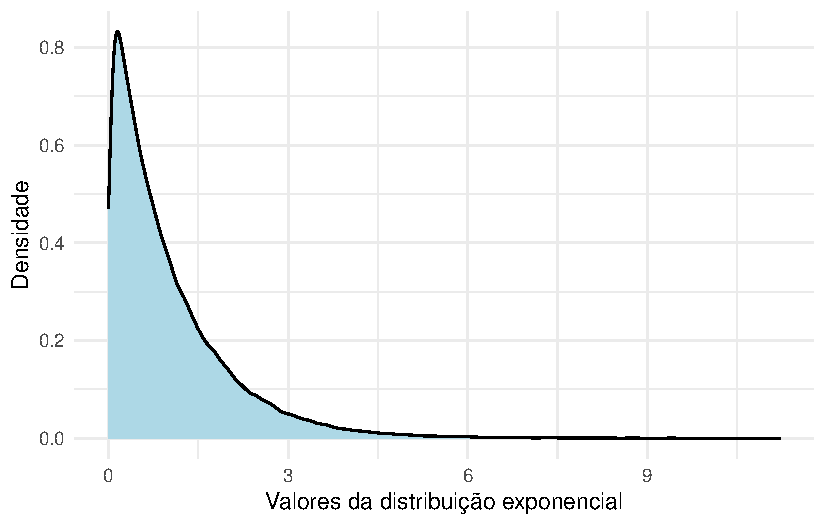
\includegraphics{./estimacao_files/figure-pdf/unnamed-chunk-16-1.pdf}

}

\end{figure}

\begin{Shaded}
\begin{Highlighting}[]
\FunctionTok{ggplot}\NormalTok{(}\FunctionTok{data.frame}\NormalTok{(}\AttributeTok{p\_chapeu =}\NormalTok{ p\_chapeus), }\FunctionTok{aes}\NormalTok{(}\AttributeTok{x =}\NormalTok{ p\_chapeu))  }\SpecialCharTok{+} 
  \FunctionTok{geom\_histogram}\NormalTok{(}
    \FunctionTok{aes}\NormalTok{(}\AttributeTok{y =} \FunctionTok{after\_stat}\NormalTok{(density)),}
    \AttributeTok{fill =} \StringTok{"steelblue"}\NormalTok{, }
    \AttributeTok{bins =} \DecValTok{15}\NormalTok{, }
    \AttributeTok{color =} \StringTok{"black"}
\NormalTok{    ) }\SpecialCharTok{+}
  \FunctionTok{coord\_cartesian}\NormalTok{(}\AttributeTok{xlim =} \FunctionTok{c}\NormalTok{(}\DecValTok{0}\NormalTok{, }\FloatTok{0.5}\NormalTok{)) }\SpecialCharTok{+}
  \FunctionTok{labs}\NormalTok{(}
    \AttributeTok{x =} \StringTok{"Proporção de gestantes ou puérperas com diarreia como sintoma"}\NormalTok{, }
    \AttributeTok{y =} \StringTok{"Densidade"}\NormalTok{,}
    \AttributeTok{title =} \StringTok{"Distribuição amostral das proporções amostrais para n = 15"}
\NormalTok{    ) }\SpecialCharTok{+} 
  \FunctionTok{geom\_vline}\NormalTok{(}\AttributeTok{xintercept =} \FunctionTok{mean}\NormalTok{(p\_chapeus), }\AttributeTok{linetype =} \DecValTok{2}\NormalTok{) }\SpecialCharTok{+}
  \FunctionTok{annotate}\NormalTok{(}
    \AttributeTok{geom =} \StringTok{"text"}\NormalTok{,}
    \AttributeTok{x =} \FloatTok{0.23}\NormalTok{, }
    \AttributeTok{y =} \DecValTok{9}\NormalTok{,}
    \AttributeTok{label =} \FunctionTok{paste}\NormalTok{(}\StringTok{"Valor médio das estimativas:"}\NormalTok{, }\FunctionTok{round}\NormalTok{(}\FunctionTok{mean}\NormalTok{(p\_chapeus), }\DecValTok{3}\NormalTok{))}
\NormalTok{    )}
\end{Highlighting}
\end{Shaded}

\begin{figure}[H]

{\centering 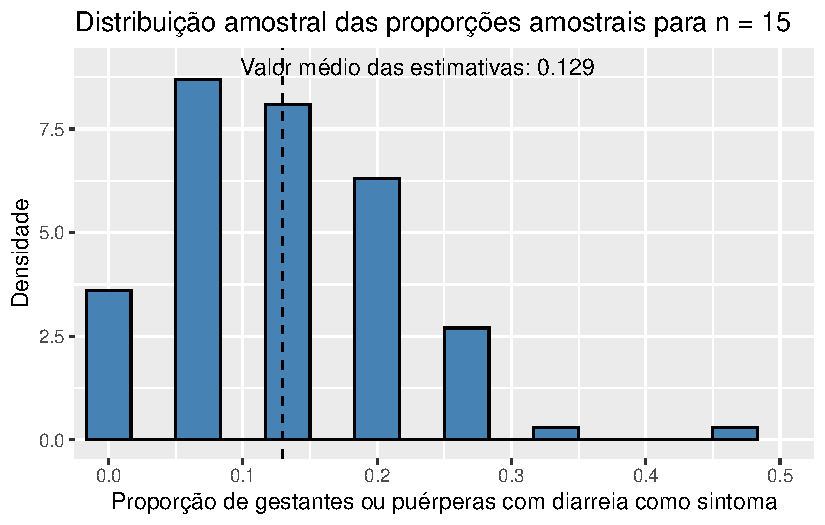
\includegraphics{./estimacao_files/figure-pdf/unnamed-chunk-16-2.pdf}

}

\end{figure}

Observando os histogramas, podemos notar que, mesmo para um tamanho de
amostra pequeno como \(n\) = 15, a distribuição de \(\bar{X}\) se
assemelha à distribuição normal, visto que apresenta o característico
formato aproximado de sino e uma quase simetria em torno de sua média.
Essa combinação de fatores nos sugere que \(X_1, X_2, ..., X_{15}\), as
variáveis aleatórias que compõem as amostras da população de idades,
seguem, também, uma distribuição simétrica em torno da média. Além
disso, o valor médio das estimativas \(\bar{x}\), de 31,843, está muito
próximo do verdadeiro valor do parâmetro populacional \(\mu\), que
sabemos ser de 31,81 anos. Esse resultado já era esperado, uma vez que a
distribuição de \(\bar{X}\) está centrada em \(\mu\). Pouco podemos
dizer, entretanto, do histograma da distribuição amostral de \(\hat{p}\)
até o momento; apenas que sua média está muito próxima do verdadeiro
valor de \(p\), que sabemos ser de 0,128, como já era esperado pelo
mesmo motivo. Aumentemos, então, o tamanho das amostras, e observemos os
resultados obtidos. Como a única modificação será o valor da variável
\texttt{n}, ocultaremos os códigos utilizados para evitar uma maior
poluição visual. Dessa forma, para \(n\) = 30, temos:

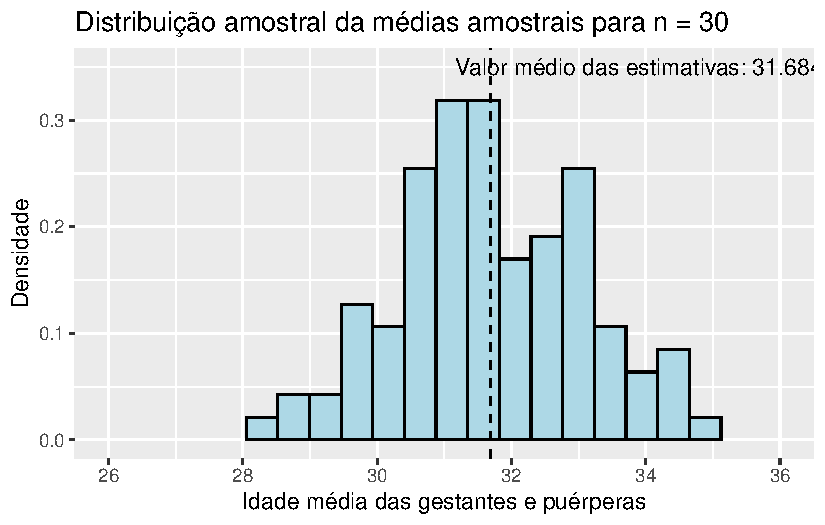
\includegraphics{./estimacao_files/figure-pdf/unnamed-chunk-17-1.pdf}

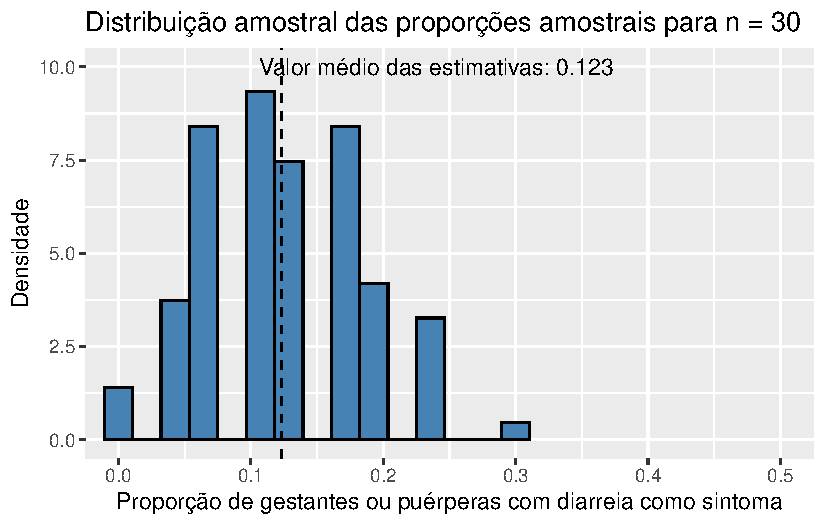
\includegraphics{./estimacao_files/figure-pdf/unnamed-chunk-17-2.pdf}

Para \(n = 50\),

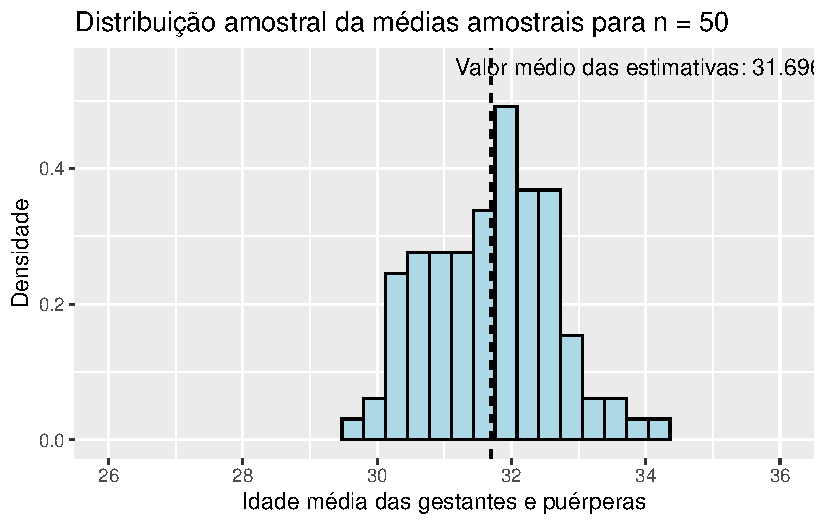
\includegraphics{./estimacao_files/figure-pdf/unnamed-chunk-18-1.pdf}

\includegraphics{./estimacao_files/figure-pdf/unnamed-chunk-18-2.pdf}

Para \(n = 100\),

\includegraphics{./estimacao_files/figure-pdf/unnamed-chunk-19-1.pdf}

\includegraphics{./estimacao_files/figure-pdf/unnamed-chunk-19-2.pdf}

Por fim, para \(n = 200\),

\includegraphics{./estimacao_files/figure-pdf/unnamed-chunk-20-1.pdf}

\includegraphics{./estimacao_files/figure-pdf/unnamed-chunk-20-2.pdf}

Observe que, conforme aumentamos o tamanho das amostras, os histogramas
de ambos os estimadores tendem a se concentrar cada vez mais em torno de
suas respectivas médias, uma vez que as variância das estimativas se
torna cada vez menor. Dessa forma, podemos concluir que estimativas
obtidas a partir de tamanhos de amostra maiores têm uma maior
probabilidade de ``acertarem'' o verdadeiro valor do parâmetro que estão
estimando. É também notável que mesmo os histogramas das proporções
amostrais aparentam convergir para o formato da distribuição normal
conforme o valor de \(n\) aumenta. Esse fato, por incrível que pareça,
não é coincidência: ele é decorrência direta do \textbf{Teorema Central
do Limite} (TCL), o qual afirma que, independente da distribuição da
população, quanto maior o tamanho amostral, mais próxima será a
distribuição amostral da média de uma distribuição normal. Vale lembrar
que a proporção amostral nada mais é do que um caso particular da média
amostral em que os valores observados na amostra contém apenas zeros e
uns, o que explica a aplicação do TCL nesse caso. Para sermos mais
precisos, podemos dizer de forma aproximada que, para tamanhos
suficientemente grandes de amostra,

\[
\bar{X} \sim N\left(\mu, \frac{\sigma^2}{n} \right) \text{ e } \hat{p}\sim N\left(p, \frac{p(1-p)}{n} \right).
\]

Com isso, aqui terminamos o conteúdo referente à estimação pontual.

\hypertarget{estimauxe7uxe3o-intervalar}{%
\section{Estimação intervalar}\label{estimauxe7uxe3o-intervalar}}

Até este ponto, todos os estimadores que apresentamos e discutimos são
pontuais, uma vez que fornecem um único valor como estimativa para o
parâmetro de interesse. Estimativas pontuais, por mais úteis que sejam,
acabam fornecendo uma informação incompleta sobre o valor estimado do
parâmetro em questão. Como estimadores são variáveis aleatórias e,
portanto, possuem uma distribuição de probabilidade, seria de nosso
interesse que a estimativa a ser apresentada levasse em consideração uma
medida de seu possível erro. Essa essa medida pode ser, por exemplo, um
intervalo relacionado à dimensão da \emph{confiança} que temos de que o
verdadeiro valor do parâmetro está sendo captado. Dessa forma, a partir
daqui, entramos no campo da \textbf{estimação intervalar}. Dentro da
Inferência Clássica, que estamos estudando neste capítulo, estimativas
intervalares se dão a partir dos chamados \textbf{intervalos de
confiança}. Intervalos de confiança incorporam, à estimativa pontual do
parâmetro, informações a respeito da variabilidade do estimador. Além
disso, eles são obtidos através da distribuição amostral de seus
estimadores, o que justifica ainda mais o conteúdo que vimos na última
subseção de estimação pontual.

Como o intuito deste livro não é conter uma porção pesada de teoria,
introduziremos o conceito de intervalos de confiança a partir de
exemplos, realizando explicações sobre os elementos envolvidos em sua
construção conforme seja necessário. Caso seja de seu interesse, já
publicamos, no site do Observatório, um texto que pode te ajudar a
entender o melhor a teoria por trás dos intervalos de confiança, que
conta também com o detalhamento de um dos principais métodos utilizados
para a construção desses intervalos: o \textbf{método da quantidade
pivotal}. O post está disponível neste link . Com isso em mente,
prossigamos para nosso primeiro exemplo: a criação de intervalos de
confiança para a média amostral.

\hypertarget{intervalos-de-confianuxe7a-para-a-muxe9dia-amostral-quando-a-variuxe2ncia-populacional-uxe9-conhecida}{%
\subsection{Intervalos de confiança para a média amostral quando a
variância populacional é
conhecida}\label{intervalos-de-confianuxe7a-para-a-muxe9dia-amostral-quando-a-variuxe2ncia-populacional-uxe9-conhecida}}

Utilizando o exemplo já apresentado na seção anterior, considere que
\(X_1, X_2, ..., X_n\) formam uma amostra aleatória da população de
idades de gestantes e puérperas hospitalizadas e falecidas em
decorrência da COVID-19 no período de março de 2020 a dezembro de 2021,
sendo \(X_i\) a variável aleatória que representa a idade da \(i\)-ésima
gestante ou puérpera sorteada, com \(i = 1, 2, ..., n\). Denotando,
novamente, por \(\mu\) a média populacional das idades dessas mulheres,
e por \(\sigma^2\) a variância populacional dessas idades, temos, ainda
que \(E(X_i) = \mu\) e \(Var(X_i) = \sigma^2\). Suponha que queiramos
estimar o valor de \(\mu\), utilizando para isso o estimador
\(\bar{X}\). Suponha também, neste primeiro exemplo, que o valor de
\(\sigma^2\) é conhecido. Note que não estamos fazendo nenhuma suposição
sobre a distribuição de probabilidade dessas variáveis. Dessa forma,
precisaremos, a partir deste ponto, impor uma restrição: o tamanho da
amostra deve ser grande o suficiente para que possamos aplicar o Teorema
Central do Limite. Caso essa restrição seja cumprida, sabemos, por meio
do TCL e de forma aproximada, que

\[
\bar{X} \sim N \left(\mu, \frac{\sigma^2}{n} \right).
\]

Subtraindo de uma variável aleatória a sua média e dividindo o resultado
por seu desvio padrão, obtemos o que chamamos de \textbf{variável
aleatória padronizadas}. Uma variável aleatória padronizada tem média
igual a zero e variância igual a um. Aplicando esse resultado em nosso
estimador, \(\bar{X}\), obtemos uma nova variável, a qual chamaremos de
\(Z\), cuja distribuição estará totalmente definida, o que será de
grande utilidade na construção de nosso intervalo. Observe.

\[
Z = \frac{\bar{X} - \mu}{\sigma/\sqrt{n}} = \frac{\sqrt{n}\left(\bar{X} - \mu\right)}{\sigma} \sim N(0, 1).
\] Como conhecemos a distribuição de probabilidade de \(Z\), podemos,
para um certo valor \(\alpha\), com \(0 < \alpha < 1\), encontrar
valores \(z_1\) e \(z_2\), com \(z_1 < z_2\), tais que

\[
P(z_1 < Z < z_2) = 1 - \alpha.  \qquad \qquad \text{(I)}
\]

Chamamos o valor \(1 - \alpha\) de \textbf{coeficiente de confiança}.
Sua interpretação será feita posteriormente. Quanto à probabilidade
acima, note que existem infinitos valores de \(z_1\) e \(z_2\) que a
satisfazem. Como queremos encontrar um intervalo que contenha os valores
mais plausíveis do parâmetro em estudo, é de nosso interesse que a
\textbf{amplitude} desse intervalo seja a menor possível, sendo a
amplitude de um intervalo definida como a diferença entre seus extremos
superior e inferior. E, para que esse interesse seja cumprido, é
necessário que os valores de \(z_1\) e \(z_2\) sejam os mais próximos
possíveis. Para distribuições simétricas em torno do zero, como é o caso
da distribuição normal padrão, podemos mostrar que a amplitude do
intervalo será mínima se os valores de \(z_1\) e \(z_2\) forem opostos,
ou seja, se \(z_1 = -z_2\). Com isso, precisamos apenas encontrar um
valor \(z\) tal que

\[
P(Z \leqslant z) = 1 - \frac{\alpha}{2}
\]

A este valor, o qual denotamos por \(z_{1 - \alpha/2}\), damos o nome de
\textbf{quantil de ordem} \(1 - \alpha/2\). Um quantil de ordem \(k\) de
uma variável aleatória, com \(0 < k < 1\), nada mais é que o ponto tal
que, quando nele aplicada a função de distribuição acumulada da
variável, a probabilidade obtida é igual a \(k\) (a ordem que o quantil
representa). Em uma situação prática, na qual teríamos um valor definido
de \(\alpha\), poderíamos utilizar uma tabela da distribuição normal
padrão para encontrar o valor de \(z_{1 - \alpha/2}\), ou mesmo utilizar
a função \texttt{qnorm()}, do pacote básico \texttt{\{stats\}}, para
realizar esse processo. A função \texttt{qnorm()}, bem como a família de
funções do R que seguem a estrutura ``qnome\_da\_distribuição()'',
representa a função quantílica: para uma dada probabilidade e para dados
valores dos parâmetros da distribuição, a função retorna o quantil cuja
ordem é a probabilidade estipulada em seus arguementos. Com isso em
mente, podemos reescrever \(z_1\) e \(z_2\) como sendo

\[
z_1 = -z_{1 - \alpha/2} \text{ e } z_2 = z_{1 - \alpha/2}.
\]

Para que a explicação acima seja melhor absorvida, observe o gráfico a
seguir, que representa a curva da densidade de probabilidade da
distribuição normal padrão.

\begin{figure}

{\centering \includegraphics[width=1\textwidth,height=\textheight]{./figuras_estimacao/normal_padrao.png}

}

\caption{\textbf{Figura 1:} Para uma confiança de (100 - \(\alpha\))\%,
a área em cada cauda da distribuição deverá ser de \(\alpha\)/2 para que
o intervalo seja o menor possível.}

\end{figure}

Voltando à probabilidade definida em \(\text{(I)}\), a atualizando com
os resultados obtidos e reescrevendo \(Z\), temos:

\[
P(z_1 < Z < z_2) = P \left(-z_{1 - \alpha/2} < \frac{\sqrt{n}\left(\bar{X} - \mu\right)}{\sigma}  < z_{1 - \alpha/2} \right)  = 1 - \alpha.
\]

Como queremos obter um intervalo de confiança para \(\mu\), precisamos
isolá-lo na expressão acima, a saber:

\[
\begin{align}
& P\left(-z_{1 - \alpha/2} < \frac{\sqrt{n}\left(\bar{X} - \mu\right)}{\sigma} < z_{1 - \alpha/2} \right) \\ & 
= P\left(-z_{1 - \alpha/2}\sigma < \sqrt{n}\left(\bar{X} - \mu\right) < z_{1 - \alpha/2}\sigma \right)  \\ &
= P\left(-z_{1 - \alpha/2}\frac{\sigma}{\sqrt{n}} < \bar{X} - \mu < z_{1 - \alpha/2}\frac{\sigma}{\sqrt{n}} \right) \\  &
= P\left(-\bar{X} + -z_{1 - \alpha/2}\frac{\sigma}{\sqrt{n}} < - \mu < -\bar{X} + z_{1 - \alpha/2}\frac{\sigma}{\sqrt{n}} \right) \\ & = P\left(\bar{X} - z_{1 - \alpha/2}\frac{\sigma}{\sqrt{n}} < \mu < \bar{X} - -z_{1 - \alpha/2}\frac{\sigma}{\sqrt{n}} \right) = 1 - \alpha
\end{align}
\] Portanto, quando a variância populacional é conhecida, um intervalo
de confiança para \(\mu\), com coeficiente de confiança \(1 - \alpha\),
é dado por

\[
IC(\mu,\ 1 - \alpha) = \left(\bar{X} - z_{1 - \alpha/2}\frac{\sigma}{\sqrt{n}};\; \bar{X} + z_{1 - \alpha/2}\frac{\sigma}{\sqrt{n}}\right).
\]

A interpretação do resultado acima deve ser feita com cuidado. É preciso
entender que a expressão \(IC(\mu,\ 1 - \alpha)\) envolve uma variável
aleatória, \(\bar{X}\), fazendo com que o intervalo obtido também seja
aleatório. Para o \textbf{intervalo aleatório} encontrado acima, podemos
dizer que a probabilidade aproximada de ele conter o verdadeiro valor do
parâmetro \(\mu\) é de \(1 - \alpha\). Aproximada, nesse caso, porque
estamos utilizando o TCL para fazer uma aproximação da distribuição de
probabilidade de \(\bar{X}\); caso a população seguisse distribuição
normal, essa probabilidade seria exata. De qualquer forma, quando
coletamos a amostra e observamos uma estimativa \(\bar{x}\), obtemos um
intervalo numérico, que chamamos de \textbf{intervalo de confiança
observado}. A partir desse ponto, não existem mais quantidades
aleatórias na expressão do intervalo, uma vez que, na Inferência
Clássica, os parâmetros, por mais que possam ser desconhecidos, são
quantidades \textbf{fixas}. Dessa forma, não podemos mais afirmar que um
intervalo de confiança observado possui probabilidade \(1 - \alpha\) de
conter o verdadeiro valor do parâmetro. Podemos apenas dizer que temos
uma \emph{confiança} considerável de que esse intervalo contém o
verdadeiro valor do parâmetro. A medida da nossa confiança é de
\(1 - \alpha\) porque, antes de colhermos a amostra, \(1 - \alpha\) era
a probabilidade aproximada de que o intervalo aleatório contivesse o
verdadeiro valor de \(\mu\).

Como a distinção entre confiança e probabilidade pode ser difícil de se
entender, uma interpretação conveniente para intervalos de confiança é a
seguinte: se obtivéssemos várias amostras de mesmo tamanho e, para cada
uma delas, calculássemos os correspondentes intervalos de confiança com
coeficiente de confiança \(1 - \alpha\), esperaríamos que a proporção de
intervalos que contivessem o verdadeiro valor do parâmetro fosse igual a
\(1 - \alpha\).

Por fim, antes de realizarmos um exemplo numérico, podemos fazer algumas
considerações a respeito da escolha do valor de \(\alpha\). É possível
mostrar que, conforme aumentamos o coeficiente de confiança, a amplitude
do intervalo aumenta. Isso, claro, é algo que deveríamos esperar, visto
que intervalos maiores possuem naturalmente uma maior chance de conterem
um valor desconhecido. Com isso, para que os intervalos sejam o mais
\emph{informativo} possível, mantendo uma confiança elevada, é
necessário que selecionemos \(\alpha\) de forma balanceada, sendo uma
escolha muito comum o valor 0,05 (nesse caso, temos que o coeficiente de
confiança é de 0,95). É muito mais interessante, por exemplo, um
intervalo de confiança que diz que o verdadeiro valor do salário médio
de um estatístico está entre 3,5 a 6 salários mínimos do que um
intervalo que diz que esse valor está entre 2 a 7,5 salários mínimos.
Apesar de, com o segundo intervalo, termos uma maior confiança de que o
verdeiro valor do salário médio está sendo captado, a qualidade da
informação que extraímos dele é consideravelmente pior do que aquela
obtida com o primeiro intervalo.

\hypertarget{um-exemplo-numuxe9rico}{%
\subsubsection{Um exemplo numérico}\label{um-exemplo-numuxe9rico}}

Substituindo as letras por números, e continuando o exemplo em que
estávamos, vamos, agora, obter, através do R, um intervalo de 95\%
confiança para \(\mu\). Lembre-se que aqui \(\mu\) é a média
populacional das idades das gestantes e puérperas hospitalizadas e
falecidas em decorrência da COVID-19 no período de março de 2020 a
dezembro de 2021. Como precisamos que nossa amostra seja suficientemente
grande para que possamos aplicar o TCL, utilizaremos \(n = 50\), uma vez
que, observando os histogramas criados na seção de Distribuição
Amostral, a distribuição de \(bar{X}\) já se aproxima satisfatóriamente
bem da distribuição normal a partir desse ponto. Além disso, como a
expressão do intervalo de confiança obtido acima leva em consideração
que a variância populacional é conhecida, precisaremos, também, dessa
informação. Para calculá-la, teremos de multiplicar o resultado da
função \texttt{var()} por \(\frac{N - 1}{N}\), sendo \(N\) o tamanho da
população, uma vez que essa função utiliza \(N - 1\) como denominador
para o cálculo da variância. Observe o código abaixo.

\begin{Shaded}
\begin{Highlighting}[]
\NormalTok{sigma2 }\OtherTok{\textless{}{-}} \FunctionTok{var}\NormalTok{(populacao1) }\SpecialCharTok{*}\NormalTok{ (}\FunctionTok{length}\NormalTok{(populacao1) }\SpecialCharTok{{-}} \DecValTok{1}\NormalTok{)}\SpecialCharTok{/}\FunctionTok{length}\NormalTok{(populacao1)}
\NormalTok{sigma2}
\end{Highlighting}
\end{Shaded}

\begin{verbatim}
[1] 45.97659
\end{verbatim}

Obtendo uma amostra de tamanho \(n = 50\) por meio da função
\texttt{sample()}, e a armazenando no vetor \texttt{amostra\_ic\_media},
temos:

\begin{Shaded}
\begin{Highlighting}[]
\FunctionTok{set.seed}\NormalTok{(}\DecValTok{34}\NormalTok{)}
\NormalTok{amostra\_ic\_media }\OtherTok{\textless{}{-}} \FunctionTok{sample}\NormalTok{(}\AttributeTok{x =}\NormalTok{ populacao1, }\AttributeTok{size =} \DecValTok{50}\NormalTok{, }\AttributeTok{replace =} \ConstantTok{TRUE}\NormalTok{)}
\FunctionTok{head}\NormalTok{(amostra\_ic\_media, }\DecValTok{20}\NormalTok{)}
\end{Highlighting}
\end{Shaded}

\begin{verbatim}
 [1] 26 39 32 35 35 35 31 21 25 40 33 32 19 22 19 30 40 31 38 36
\end{verbatim}

Nesse próximo passo, criaremos uma função, a qual chamaremos de
\texttt{ic\_media\_caso1()}, que calculará intervalos de confiança para
o parâmetro \(\mu\) quando a variância populacional é conhecida e
\(\bar{X}\) segue distribuição normal (ou aproximadamente normal). A
função possuirá três argumentos: \texttt{dados}, que receberá o vetor de
valores observados na amostra; \texttt{sigma}, que receberá o valor do
desvio padrão populacional; e \texttt{alpha}, que receberá o valor
necessário para se obter o coeficiente de confiança associado ao
intervalo, que nesse caso será de 0,05. Utilizaremos a já explicada
função \texttt{qnorm()} para encontrar o valor do quantil de ordem
\(1 - \alpha\) da normal padrão (não utilizaremos os argumentos
\texttt{mean} e \texttt{sigma} dessa função, uma vez que seus valores
padrões são, respectivamente, 1 e 0). O limite inferior do intervalo
será guardado no vetor \texttt{limite\_inferior}, enquanto o superior
será guardado em \texttt{limite\_superior}. A função retornará um data
frame contendo algumas medidas referentes à amostra e o intervalo de
confiança propriamente dito. O resultado do processo pode ser visto
abaixo.

\begin{Shaded}
\begin{Highlighting}[]
\NormalTok{ic\_media\_caso1 }\OtherTok{\textless{}{-}} \ControlFlowTok{function}\NormalTok{(amostra, sigma, alfa) \{}
\NormalTok{  media }\OtherTok{\textless{}{-}} \FunctionTok{mean}\NormalTok{(amostra)}
\NormalTok{  n }\OtherTok{\textless{}{-}} \FunctionTok{length}\NormalTok{(amostra)}
\NormalTok{  z }\OtherTok{\textless{}{-}} \FunctionTok{round}\NormalTok{(}\FunctionTok{qnorm}\NormalTok{(}\AttributeTok{p =} \DecValTok{1} \SpecialCharTok{{-}}\NormalTok{ alfa}\SpecialCharTok{/}\DecValTok{2}\NormalTok{), }\DecValTok{3}\NormalTok{)}
\NormalTok{  limite\_inferior }\OtherTok{\textless{}{-}} \FunctionTok{round}\NormalTok{(media }\SpecialCharTok{{-}}\NormalTok{ z }\SpecialCharTok{*}\NormalTok{ sigma}\SpecialCharTok{/}\FunctionTok{sqrt}\NormalTok{(n), }\DecValTok{3}\NormalTok{)}
\NormalTok{  limite\_superior }\OtherTok{\textless{}{-}} \FunctionTok{round}\NormalTok{(media }\SpecialCharTok{+}\NormalTok{ z }\SpecialCharTok{*}\NormalTok{ sigma}\SpecialCharTok{/}\FunctionTok{sqrt}\NormalTok{(n), }\DecValTok{3}\NormalTok{)}
\NormalTok{  amplitude }\OtherTok{\textless{}{-}}\NormalTok{ limite\_superior }\SpecialCharTok{{-}}\NormalTok{ limite\_inferior}
  \FunctionTok{return}\NormalTok{(}
    \FunctionTok{data.frame}\NormalTok{(}
\NormalTok{      n, }
      \AttributeTok{estimativa\_pontual =}\NormalTok{ media,}
\NormalTok{      limite\_inferior, }
\NormalTok{      limite\_superior,}
\NormalTok{      amplitude)}
\NormalTok{    )}
\NormalTok{\}}

\FunctionTok{ic\_media\_caso1}\NormalTok{(}\AttributeTok{amostra =}\NormalTok{ amostra\_ic\_media, }\AttributeTok{sigma =} \FunctionTok{sqrt}\NormalTok{(sigma2), }\AttributeTok{alfa =} \FloatTok{0.05}\NormalTok{)}
\end{Highlighting}
\end{Shaded}

\begin{verbatim}
   n estimativa_pontual limite_inferior limite_superior amplitude
1 50              32.16          30.281          34.039     3.758
\end{verbatim}

Portanto, um intervalo de 95\% de confiança para a média populacional
das idades das gestantes e puérperas hospitalizadas e falecidas em
decorrência da COVID-19 no período em estudo é de (28,401; 32,159).
Intervalos de confiança podem, inclusive, ser utilizados como
substitutos para \textbf{testes de hipóteses}, dos quais falaremos no
próximo capítulo. Caso quiséssemos, por exemplo, testar a hipótese de
que o valor de \(\mu\) é igual a 27, rejeitaríamos a hipótese nula sob
um nível de significância de 0,05, uma vez que 27 não está contido no
intervalo de 95\% de confiança para \(\mu\) obtido acima.

\hypertarget{intervalos-de-confianuxe7a-para-a-muxe9dia-amostral-quando-a-variuxe2ncia-populacional-uxe9-desconhecida}{%
\subsection{Intervalos de confiança para a média amostral quando a
variância populacional é
desconhecida}\label{intervalos-de-confianuxe7a-para-a-muxe9dia-amostral-quando-a-variuxe2ncia-populacional-uxe9-desconhecida}}

Considere, assim como no exemplo anterior, que \(X_1, X_2, ..., X_n\)
formam uma amostra aleatória da população de idades de gestantes e
puérperas hospitalizadas e falecidas em decorrência da COVID-19 no
período de março de 2020 a dezembro de 2021, sendo \(X_i\) a variável
aleatória que representa a idade da \(i\)-ésima gestante ou puérpera
sorteada, com \(i = 1, 2, ..., n\). Suponha que queiramos, novamente,
estimar o valor de \(\mu\), mas que agora o valor da variância
populacional \(\sigma^2\) é desconhecido. Ainda com a restrição de que o
tamanho da amostra deve ser suficientemente grande para que possamos
aplicar o Teorema Central do Limite, sabemos, como visto anteriormente,
que

\[
Z  = \frac{\sqrt{n}\left(\bar{X} - \mu\right)}{\sigma} \sim N(0, 1).
\]

Lembre-se, entretanto, que estamos no caso em que \(\sigma^2\) é
desconhecido, e por isso não podemos utilizar a variável acima para
construirmos o intervalo de confiança, uma vez que o intervalo
encontrado seria função de \(\sigma\). Dessa forma, é intuitivo que em
algum momento utilizemos um estimador da variância populacional na
expressão do intervalo. Por sorte, existe um conhecido resultado dentro
da Estatística que fornecerá uma função que nos seja conveniente.
Definindo, primeiramente, o \textbf{estimador da variância amostral},
denotado por \(S^2\), como sendo

\[
S^2 = \frac{\sum_{i = 1}^n (X_i - \bar{X})}{n - 1},
\] sabemos ser válido que

\[
T = \frac{\sqrt{n} \left(\bar{X} - \mu \right)}{S} \sim t_{n - 1},
\] onde \(S\) é a raiz quadrada de \(S^2\) e \(t_{n - 1}\) representa a
distribuição de probabilidade T de Student com \(n - 1\) graus de
liberdade. A demonstração desse resultado pode ser consultada no post do
Observatório que referenciamos no início da seção. A partir daqui, o
processo para obtermos a expressão do intervalo de confiança será muito
semelhante ao que realizamos no exemplo anterior. Como a distribuição da
variável aleatória \(T\) é totalmente conhecida, uma vez que, em uma
situação prática, o valor do tamanho da amostra \(n\) estaria definido,
podemos encontrar valores \(t_{1_{(n-1)}}\) e \(t_{2_{(n-1)}}\), com
\(t_{1_{(n-1)}} < t_{2_{(n-1)}}\), tais que

\[
P\left(t_{1_{(n-1)}} < T < t_{2_{(n-1)}} \right) = 1 - \alpha. \qquad \qquad \text{(II)}
\]

Como a distribuição T de Student, assim como a distribuição normal
padrão, é simétrica em torno de zero, os valores de \(t_1\) e \(t_2\)
que geram a menor amplitude possível para o intervalo de confiança serão
dados por

\[
t_{1_{(n-1)}} = -t_{(n - 1;\;1 -\alpha/2)} \text{ e } t_{2_{(n-1)}} = t_{(n - 1;\;1 -\alpha/2)}.
\]

Em outras palavras, para encontrarmos os valores desses pontos, basta
que calculemos o quantil de ordem \(1 - \alpha/2\) da distribuição T de
Student com \(n - 1\) graus de liberdade. Voltando à probabilidade
definida em \(\text{(II)}\), a atualizando com os resultados obtidos e
reescrevendo \(T\), temos:

\[
P\left(t_{1_{(n-1)}} < T < t_{2_{(n-1)}} \right) = P\left(-t_{(n - 1;\;1 -\alpha/2)} < \frac{\sqrt{n}\left(\bar{X} - \mu\right)}{S} < -t_{(n - 1;\;1 -\alpha/2)} \right) = 1 - \alpha.
\]

Como queremos obter um intervalo de confiança para \(\mu\), precisamos
isolá-lo na expressão acima, a saber:

\[
\begin{align}
& P\left(-t_{(n - 1;\;1 -\alpha/2)} < \frac{\sqrt{n}\left(\bar{X} - \mu\right)}{S} < t_{(n - 1;\;1 -\alpha/2)} \right) \\ & 
= P\left(-t_{(n - 1;\;1 -\alpha/2)} S < \sqrt{n}\left(\bar{X} - \mu\right) < t_{(n - 1;\;1 -\alpha/2)} S\right) \\ & = 
P\left(-t_{(n - 1;\;1 -\alpha/2)} \frac{S}{\sqrt{n}} < \bar{X} - \mu < t_{(n - 1;\;1 -\alpha/2)} \frac{S}{\sqrt{n}} \right) \\ & = 
P\left(-\bar{X} + -t_{(n - 1;\;1 -\alpha/2)} \frac{S}{\sqrt{n}} < - \mu < -\bar{X} + t_{(n - 1;\;1 -\alpha/2)} \frac{S}{\sqrt{n}} \right) \\ & 
= P\left(\bar{X} - t_{(n - 1;\;1 -\alpha/2)} \frac{S}{\sqrt{n}} < \mu < \bar{X} - -t_{(n - 1;\;1 -\alpha/2)} \frac{S}{\sqrt{n}} \right) = 1 - \alpha
\end{align} 
\]

Portanto, quando a variância populacional é desconhecida, um intervalo
de confiança para \(\mu\), com coeficiente de confiança de
\(1 - \alpha\), é dado por

\[
IC(\mu,\ 1 - \alpha) = \left(\bar{X} - t_{(n-1;\;1 - \alpha/2)} \frac{S}{\sqrt{n}}; \bar{X} + t_{(n-1;\;1 - \alpha/2)} \frac{S}{\sqrt{n}} \right).
\]

Algo interessante a se observar é que, tanto o intervalo aleatório
acima, quanto o intervalo aleatório encontrado no exemplo anterior,
possuem probabilidade 1 - \(\alpha\) de conterem o verdadeiro valor do
parâmetro \(\mu\), mesmo que suas estruturas sejam diferentes.
Entretanto, como na construção do intervalo apresentado no presente
exemplo foi utilizado um estimador de \(\sigma\), a amplitude média dos
intervalos de confiança obtidos por esse método será maior do que a
amplitude média dos intervalos obtidos quando utilizamos o método
apresentado no exemplo anterior. Com isso, dizemos que o intervalo de
confiança acima é menos informativo, uma vez que o intervalo de valores
plausíveis para \(\mu\), nesse caso, será maior que o do intervalo de
confiança construído anteriormente. Esse problema é mais evidente para
tamanhos pequenos de amostra, e torna-se menos relevante conforme o
valor de \(n\) aumenta.

\hypertarget{um-exemplo-numuxe9rico-1}{%
\subsubsection{Um exemplo numérico}\label{um-exemplo-numuxe9rico-1}}

Para demonstrar a diferença entre o intervalo de confiança derivado
acima e aquele derivado no exemplo anterior, podemos aproveitar o mesmo
exemplo sobre a média das idades das gestantes e puérperas previamente
discutido. Novamente, criaremos uma função, a qual chamaremos de
\texttt{ic\_media\_caso2()}, que retornará o intervalo de confiança para
a média populacional quando a variância populacional é desconhecida e
\(\bar{X}\) segue distribuição normal (ou aproximadamente normal). A
função se dará de forma similar àquela criada anteriormente, sendo as
únicas diferenças o cálculo do desvio padrão amostral, feito com a
função \texttt{sd()}, do pacote básico \texttt{\{stats\}} e a obtenção
do quantil da distribuição T de Student através da função \texttt{qt()},
do mesmo pacote. O resultado do processo pode ser visto abaixo.
Lembre-se que o vetor \texttt{amostra\_ic\_media} foi criado no exemplo
anterior.

\begin{Shaded}
\begin{Highlighting}[]
\NormalTok{ic\_media\_caso2 }\OtherTok{\textless{}{-}} \ControlFlowTok{function}\NormalTok{(dados, alfa) \{}
\NormalTok{  media }\OtherTok{\textless{}{-}} \FunctionTok{mean}\NormalTok{(dados)}
\NormalTok{  n }\OtherTok{\textless{}{-}} \FunctionTok{length}\NormalTok{(dados)}
\NormalTok{  S }\OtherTok{\textless{}{-}} \FunctionTok{round}\NormalTok{(}\FunctionTok{sd}\NormalTok{(dados), }\DecValTok{3}\NormalTok{)}
\NormalTok{  t }\OtherTok{\textless{}{-}} \FunctionTok{qt}\NormalTok{(}\DecValTok{1} \SpecialCharTok{{-}}\NormalTok{ alfa}\SpecialCharTok{/}\DecValTok{2}\NormalTok{, n }\SpecialCharTok{{-}} \DecValTok{1}\NormalTok{)}
\NormalTok{  limite\_inferior }\OtherTok{\textless{}{-}} \FunctionTok{round}\NormalTok{(media }\SpecialCharTok{{-}}\NormalTok{ t }\SpecialCharTok{*}\NormalTok{ S}\SpecialCharTok{/}\FunctionTok{sqrt}\NormalTok{(n), }\DecValTok{3}\NormalTok{)}
\NormalTok{  limite\_superior }\OtherTok{\textless{}{-}} \FunctionTok{round}\NormalTok{(media }\SpecialCharTok{+}\NormalTok{ t }\SpecialCharTok{*}\NormalTok{ S}\SpecialCharTok{/}\FunctionTok{sqrt}\NormalTok{(n), }\DecValTok{3}\NormalTok{)}
\NormalTok{  amplitude }\OtherTok{\textless{}{-}}\NormalTok{ limite\_superior }\SpecialCharTok{{-}}\NormalTok{ limite\_inferior}
  \FunctionTok{return}\NormalTok{(}
    \FunctionTok{data.frame}\NormalTok{(}
\NormalTok{      n,}
\NormalTok{      S, }
      \AttributeTok{estimativa\_pontual =}\NormalTok{ media,}
\NormalTok{      limite\_inferior,}
\NormalTok{      limite\_superior,}
\NormalTok{      amplitude)}
\NormalTok{    )}
\NormalTok{\}}

\FunctionTok{ic\_media\_caso2}\NormalTok{(}\AttributeTok{dados =}\NormalTok{ amostra\_ic\_media, }\AttributeTok{alfa =} \FloatTok{0.05}\NormalTok{)}
\end{Highlighting}
\end{Shaded}

\begin{verbatim}
   n     S estimativa_pontual limite_inferior limite_superior amplitude
1 50 6.634              32.16          30.275          34.045      3.77
\end{verbatim}

Como podemos perceber, o intervalo de confiança obtido acima apresenta
uma amplitude levemente maior do que o intervalo obtido anteriormente
(3,77 contra 3,758). Dessa forma, apesar de a diferença não ser
gritante, podemos perceber que a utilização de uma estimativa para o
valor da variância populacional acarretou, como já explicado
anteriormente, em um intervalo levemente menos informativo a respeito do
verdadeiro valor da média populacional. Essa diferença na amplitude,
entretanto, não é regra: poderíamos ter coletado uma amostra em que a
amplitude do intervalo de confiança construído pelo presente método
fosse menor. Além disso, como o tamanho da amostra é grande o
suficiente, a diferença nas amplitudes dos dois intervalos passa a ser
praticamente desconsiderável. Com isso, aqui encerramos a construção de
intervalos de confiança para a média de uma população. Partamos, agora,
para a última seção desse capítulo, na qual trataremos da obtenção de
intervalos de confiança para a proporção populacional.

\hypertarget{intervalos-de-confianuxe7a-para-a-proporuxe7uxe3o-populacional}{%
\subsection{Intervalos de confiança para a proporção
populacional}\label{intervalos-de-confianuxe7a-para-a-proporuxe7uxe3o-populacional}}

A fazer

\bookmarksetup{startatroot}

\hypertarget{testes-nuxe3o-paramuxe9tricos}{%
\chapter{Testes não-paramétricos}\label{testes-nuxe3o-paramuxe9tricos}}

Testes não paramétricos são testes estatísticos usados quando as
suposições de um teste paramétrico não são atendidas, principalmente
quando os dados não são normalmente distribuídos. Por estes testes não
exigirem suposições muito fortes em relação à distribuição dos dados,
eles tendem a ser menos poderosos que os testes paramétricos.

Geralmente, a suposição de normalidade dos dados é violada quando o
tamanho do grupo ou amostra é pequeno, ou quando os dados são
assimétricos. Nesses casos, os resultados de um teste paramétrico podem
não ser confiáveis, dado que suposições importantes relacionadas ao
tamanho do grupo e simetria dos dados estarão sendo violadas, o que irá
comprometer o teste.

Os testes não-paramétricos são geralmente divididos conforme a
quantidade de grupos sendo estudados. Os testes para um único grupo
costumam ser utilizados para verificar se os dados são originados de uma
população com alguma distribuição ou característica populacional
específica, como a média ou mediana, por exemplo. Por outro lado, em
testes para dois ou mais grupos podemos compará-los de acordo com algum
critério específico do teste em questão. Tais testes de dois ou mais
grupos são os quais iremos nos concentrar ao longo deste capítulo.

Serão apresentados alguns dos testes não-paramétricos mais utilizados na
área da saúde, sendo testes para grupos pareados e não-pareados. Além
disso, devemos lembrar que os testes que serão apresentados não são os
únicos, sendo importante avaliar com cuidado o problema que está sendo
estudado para escolher o teste adequado.

\hypertarget{grupos-nuxe3o-pareados}{%
\section{Grupos não-pareados}\label{grupos-nuxe3o-pareados}}

Para grupos não-pareados ou independentes, dentre os testes mais
conhecidos e utilizados temos os testes de Mann-Whitney e
Kolmogorov-Smirnov para dois grupos, e o de Kruskal-Wallis para três ou
mais grupos.

\hypertarget{teste-de-mann-whitney}{%
\subsection{Teste de Mann-Whitney}\label{teste-de-mann-whitney}}

O teste de Mann-Whitney é um teste estatístico não paramétrico usado
para comparar dois grupos independentes, sendo o grau de medida pelo
menos ordinal para variável de interesse e nominal para variável
independente. Além disso, o teste é geralmente usado quando a variável
resposta ou de interesse não é normalmente distribuída, sendo assim, uma
alternativa não-paramétrica ao teste t para amostras independentes.

Quando o resultado do teste for significativo, significa que ambos os
grupos representam populações com distribuições diferentes. Caso a
suposição de que ambas as distribuições são iguais seja feita, então
podemos interpretar o teste como uma comparação de medianas, que ao ser
significativo dizemos que as medianas são significativamente diferentes.
Assim, considerando dois grupos independentes, as hipóteses podem ser
definidas como:

\(H_0:\) distribuição\(_1=\) distribuição\(_2\)

\(H_{\mathrm{a}}:\) distribuição\(_1 \neq\) distribuição\({ }_2\)

Suponha que queremos comparar as idades (anos) de gestantes
hospitalizadas com Covid-19 de dois hospitais diferentes. Considere as
idades coletadas nos seguintes grupos:

Hospital A: {\(\quad 46,48,34,36,22,44,50\)}

Hospital B: \(\quad 25,21,39,14,37\)

Confirmado que o teste de Mann-Whitney é apropriado, o primeiro passo
que devemos tomar, é ordenar os valores de ambos os grupos de forma
crescente em um único grupo, e então, identificar o posto de cada valor
desse grupo. Para o exemplo abordado, teremos o seguinte:

\begin{array}{llllllllllll}
\hline \text { Idades } & 14 & 21 & \color{red}{22} & 25 & \color{red}{34} & \color{red}{36} & 37 & 39 & \color{red}{44} & \color{red}{46} & \color{red}{48} & \color{red}{50}\\
\hline \text { Posto } & 1 & 2 & \color{red}{3} & 4 & \color{red}{5} & \color{red}{6} & 7 & 8 & \color{red}{9} & \color{red}{10} & \color{red}{11} & \color{red}{12}\\
\hline
\end{array}

Onde está destacado em vermelho as idades das gestantes hospitalizadas
no Hospital A e seus respectivos postos. Além disso, destacado em preto
essa mesma informação para as gestantes hospitalizadas no Hospital B.

\hypertarget{estatuxedstica-u}{%
\subsubsection{\texorpdfstring{Estatística
\(U\)}{Estatística U}}\label{estatuxedstica-u}}

O teste de Mann-Whitney também é chamado de teste \(U\) de Mann-Whitney,
pois calculamos o que chamamos de estatística \(U\), a qual é uma
quantidade baseada na soma dos postos identificados de cada grupo
calculada para fazer a avaliação das hipóteses.

Agora, considere \(n_1\) e \(n_2\) como o número de observações do grupo
1 e grupo 2 respectivamente, em que, o grupo 1 será aquele com o menor
número de observações (caso ambos os grupos tenham a mesma quantidade de
observações, então \(n_1 = n_2\)). Além disso, considere \(R_1\) e
\(R_2\) como a soma dos postos identificados nos grupos 1 e 2
respectivamente, e \(N = n_1 + n_2\) como o total de observações
considerando ambos os grupos.

Definido os termos necessários e considerando o exemplo apresentado,
calculamos as seguintes quantidades:

\(U_1=n_1n_2+\displaystyle \frac{n_1\left(n_1+1\right)}{2}-R_1=5\cdot7+\displaystyle \frac{5 \cdot\left(5+1\right)}{2}-22 = 28\),

\(U_2=n_1 n_2+\displaystyle \frac{n_2\left(n_2+1\right)}{2}-R_2=5 \cdot 7+\displaystyle \frac{7 \cdot\left(7+1\right)}{2}-56 = 7\).

Tendo calculado \(U_1\) e \(U_2\) a estatística \(U\) será o menor valor
entre ambas, neste caso, \(U = U_2\). Podemos confirmar se todo
procedimento foi feito corretamente ao verificar a relação
\(n_1n_2 = U_1 + U_2\), a qual será \(5\cdot 7 = 28 + 7 = 35\) no
exemplo considerado.

\hypertarget{avaliauxe7uxe3o-das-hipuxf3teses}{%
\subsubsection{Avaliação das
hipóteses}\label{avaliauxe7uxe3o-das-hipuxf3teses}}

Para avaliar as hipóteses precisamos calcular a quantidade \(U_c\), o
qual é o valor crítico de \(U\) necessário para decidir em relação às
hipóteses. Este valor pode ser encontrado em tabelas de valores críticos
da estatística U bilateral (ou unilateral a depender das hipóteses), ou
podemos utilizar a função \texttt{qwilcox()} do R e subtrair o resultado
por 1, para obtê-lo no caso bilateral. Para o exemplo dos hospitais
temos \(n_1 = 5\) e \(n_2 = 7\), considerando nível de 5\% de
significância, podemos utilizar a função \texttt{qwilcox()} para
encontrar \(U_c\) da seguinte forma:

\begin{Shaded}
\begin{Highlighting}[]
\FunctionTok{qwilcox}\NormalTok{(}\FloatTok{0.05}\SpecialCharTok{/}\DecValTok{2}\NormalTok{,}\DecValTok{5}\NormalTok{,}\DecValTok{7}\NormalTok{) }\SpecialCharTok{{-}} \DecValTok{1}
\end{Highlighting}
\end{Shaded}

\begin{verbatim}
[1] 5
\end{verbatim}

Onde \(0.05/2\) é o nível de significância dividido por dois devido ao
teste ser bilateral, e subtraímos por \(1\) como uma correção matemática
por \(U\) ser discreto e \texttt{qwilcox()} calcular quantis, e não
valores críticos de \(U\). Assim, \(U_c = 5\) no exemplo considerado.

Assim, rejeitamos a hipótese nula quando o valor da estatística \(U\)
calculada for menor ou igual ao valor crítico de \(U\), ou seja, quando
\(U \leq U_c\). Com os valores calculados de \(U = 7\) e \(U_c = 5\),
podemos concluir ao nível de 5\% de significância que não há diferença
significativa entre as distribuições das idades das gestantes
hospitalizadas em ambos hospitais.

\hypertarget{empates}{%
\subsubsection{Empates}\label{empates}}

Dependendo do problema, pode existir valores repetidos observados, e ao
ordená-los para identificar os postos, esses valores são considerados
empates.

\begin{array}{llllllllllll}
\hline \text { Idades } & 14 & 21 & \color{red}{25} & \color{red}{25} & \color{red}{34} & \color{red}{36} & 37 & 39 & \color{red}{44} & \color{red}{46} & \color{red}{48} & \color{red}{50}\\
\hline \text { Posto } & 1 & 2 & \color{red}{3,5} & \color{red}{3,5} & \color{red}{5} & \color{red}{6} & 7 & 8 & \color{red}{9} & \color{red}{10} & \color{red}{11} & \color{red}{12}\\
\hline
\end{array}

Observe nesse exemplo que há um empate para idade de 25 anos. Nesse
caso, ao ordenar os valores teríamos os postos 3 e 4 para esses valores
repetidos, mas devemos atribuir a média desses postos para dar
continuidade ao teste. Assim, temos
\(\displaystyle \frac{3 + 4}{2}= 3,5\).

\hypertarget{estatuxedstica-u-normalizada}{%
\subsubsection{\texorpdfstring{Estatística \(U\)
normalizada}{Estatística U normalizada}}\label{estatuxedstica-u-normalizada}}

É tido como um consenso a utilização dos procedimentos apresentados até
então sobre o teste Mann-Whitney no cenário em que \(n_1\) e \(n_2\) são
menores ou iguais que 20. Por outro lado, no cenário em que \(n_1\) e
\(n_2\) são grandes (\(>20\)), podemos aproximar a distribuição de \(U\)
para uma normal. Assim, calculamos a estatística \(Z_u\) para avaliar as
hipóteses da seguinte forma:

\[Z_u = \displaystyle \frac{U-\displaystyle\frac{n_1  n_2}{2}}{\sqrt{\displaystyle\frac{n_1 n_2\left(n_1+n_2+1\right)}{12}}}.\]

Esse procedimento nada mais é do que subtrair a média de \(U\) e dividir
pelo seu desvio padrão.

Assim, para avaliar as hipóteses, é necessário obter o valor crítico de
\(Z_u\), o qual pode ser obtido a partir de tabelas de valores críticos
da distribuição normal padrão, ou podemos recorrer à função
\texttt{qnorm()} no R com os seguintes argumentos:
\texttt{qnorm(0.05/2,\ lower.tail\ =\ FALSE)} para teste bilateral e
nível de 5\% de significância;
\texttt{qnorm(0.05,\ lower.tail\ =\ FALSE)} para teste unilateral e
nível de 5\% de significância. Os valores críticos de \(Z_u\) para o
teste bilateral e unilateral ao nível de 5\% de significância são 1,96 e
1,65 respectivamente. Assim, rejeitamos a hipótese nula quando
\(|Z_u|\geq1,96\) e \(|Z_u|\geq1,65\) no teste bilateral e unilateral
respectivamente.

Caso haver empates, a aproximação deve ser feita da seguinte forma:

\[Z_u = \displaystyle \frac{U-\displaystyle\frac{n_1  n_2}{2}}{\sqrt{\displaystyle\frac{n_1n_2\left(n_1+n_2+1\right)}{12}- \displaystyle\frac{n_1n_2\left[\sum_{i=1}^s\left(t_i^3-t_i\right)\right]}{12  \left(n_1+n_2\right) \left(n_1+n_2-1\right)}}},\]

Onde, na quantidade \(\sum_{i=1}^s\left(t_i^3-t_i\right)\) o \(s\)
indica quantos grupos de empates ocorreram, ex: idade 25 se repete duas
vezes e idade 45 se repete cinco vezes, totalizando 2 grupos de empates
ou de repetições. Além disso, o termo \(t\) é o número total de empates
no grupo de repetições \(i\). Assim, para as repetições hipotéticas da
idade 25 e 45 teremos:

\[\sum_{i=1}^2\left(t_i^3-t_i\right) = (2^3 - 2) + (5^3 - 5) = 126.\]

Dessa forma, podemos calcular \(Z_u\) e então avaliar as hipóteses da
mesma forma que avaliamos no cenário sem empates.

\hypertarget{como-aplicar-o-teste-no-r}{%
\subsubsection{Como aplicar o teste no
R}\label{como-aplicar-o-teste-no-r}}

Na prática, tendo os dados em um formato de planilha, podemos
carregá-los no software R e então aplicar o teste recorrendo a uma
função específica, a qual irá efetuar os procedimentos formalmente
explicados ao longo do texto e retornar um \emph{valor-p}, o qual
podemos utilizar para avaliar as hipóteses, onde, rejeitamos a hipótese
nula caso \emph{valor-p} \(\leq 0,05\), sendo 5\% de nível de
significância escolhido. Podemos usar a seguinte estrutura:

\begin{Shaded}
\begin{Highlighting}[]
\NormalTok{stats}\SpecialCharTok{::}\FunctionTok{wilcox.test}\NormalTok{(x, y, }\AttributeTok{correct =} \ConstantTok{FALSE}\NormalTok{,  }\AttributeTok{alternative =} \StringTok{"two.sided"}\NormalTok{)}
\end{Highlighting}
\end{Shaded}

Os argumentos \texttt{x} e \texttt{y} são os vetores dos valores dos
grupos a serem comparados. O argumento \texttt{correct} indica se o
usuário quer que seja feito uma correção de continuidade do
\emph{valor-p} no caso de aproximação normal da estatística \(U\), o que
geralmente não é feito, a menos que a estatística \(Z_u\) esteja muito
próxima do valor crítico utilizado. E por fim, o argumento
\texttt{alternative} permite escolher o formato do teste de hipóteses
desejado.

\hypertarget{teste-de-kolmogorov-smirnov}{%
\subsection{Teste de
Kolmogorov-Smirnov}\label{teste-de-kolmogorov-smirnov}}

Assim como o teste de Mann-Whitney, o teste de Kolmogorov-Smirnov é uma
alternativa não paramétrica ao teste t para grupos independentes quando
há a suspeita de não normalidade da variável de interesse. O teste
possui grau de medida pelo menos ordinal, e é sensível a qualquer
diferença de tendência central, dispersão, simetria ou curtose das
distribuições.

Visa verificar se ambos os grupos originaram-se de populações com a
mesma distribuição. Para isso, é calculado a estatística de teste \(D\)
a partir das distribuições de frequências acumuladas dos grupos, e
então, utiliza-se essa estatística \(D\) para avaliar as hipóteses.
Quanto maior a estatística, maior será a evidência para rejeitar a
hipótese nula.

Retornando ao exemplo das idades de gestantes hospitalizadas com
Covid-19 em dois diferentes hospitais, as hipóteses para o teste
bilateral terão a seguinte forma:

\(H_0:\) distribuição\(_1=\) distribuição\(_2\)

\(H_{\mathrm{a}}:\) distribuição\(_1 \neq\) distribuição\({ }_2\)

São hipóteses com formas idênticas as do teste de Mann-Whitney. Porém,
embora tenham o mesmo objetivo de comparar as distribuições para ambos
os grupos, o método difere consideravelmente. Além disso, o teste de
Mann-Whitney é sensível em relação à mediana, enquanto o teste de
Kolmogorov-Smirnov é sensível em relação aos aspectos gerais das
distribuições sendo testadas como foi discutido anteriormente.

Embora seja o mesmo exemplo, serão considerados valores diferentes por
motivos didáticos:

Hospital A: \(\quad 22,22,25,27,29\)

Hospital B: \(\quad 27,31,34,37,44\)

Considerando as notações introduzidas no desenvolvimento do teste de
Mann-Whitney, os tamanhos dos grupos são \(n_1 = 5\) e \(n_2 = 5\). Vale
lembrar que, usualmente, denotamos \(n_1\) como sendo o tamanho do menor
grupo, chamado de grupo 1. Como neste exemplo ambos possuem o mesmo
tamanho, o grupo 1 sera composto dos valores das idades referentes as
gestantes hospitalizadas no Hospital A.

\hypertarget{estatuxedstica-d}{%
\subsubsection{\texorpdfstring{Estatística
\(D\)}{Estatística D}}\label{estatuxedstica-d}}

Precisamos calcular a estatística \(D\) para avaliar as hipóteses. Essa
estatística nada mais é do que o maior valor que encontrarmos ao
realizar a diferença entre as proporções de frequências relativas
acumuladas dos dois grupos. Para isso, construímos a seguinte tabela:

\begin{array}{ccccc}
\hline 
\text{Idades}_1 & S_1 & \text{Idades}_2 & S_2 & S_1-S_2 \\
\hline 22;22 & 2 / 5=0,40 & - & 0 & 0,40-0=0,40 \\
25 & 3 / 5=0,60 & - & 0 & 0,60-0=0,60 \\
27 & 4 / 5=0,80 & 27 & 1 / 5=0,20 & 0,80-0,20=0,60 \\
29 & 5 / 5=1,00 & - & 1 / 5=0,20 & 1,00-0,20=\color{red}{0,80} \\
- & 5 / 5=1,00 & 31 & 2 / 5=0,40 & 1,00-0,40=0,60 \\
- & 5 / 5=1,00 & 34 & 3 / 5=0,60 & 1,00-0,60=0,40 \\
- & 5 / 5=1,00 & 37 & 4 / 5=0,80 & 1,00-0,80=0,20 \\
- & 5 / 5=1,00 & 44 & 5 / 5=1.00 & 1,00-1,00=0,00 \\
\hline
\end{array}

As colunas Idades\textsubscript{1} e Idades\textsubscript{2} são
referentes aos valores do grupo 1 (usualmente o menor grupo, o que não é
o caso, pois \(n_1 = n_2\)) e grupo 2 respectivamente. Porém, note que
existe um valor repetido (Idades\textsubscript{1} \(= 22\)) na primeira
coluna, quando isso ocorre todas as repetições desse mesmo valor
permanecem na mesma linha. Além disso, observe que na primeira linha e
coluna Idades\textsubscript{2} foi atribuído um símbolo de \(-\), isso
ocorre, pois não há um valor de Idades\textsubscript{2} \(= 22\) assim
como na coluna Idades\textsubscript{1}. O mesmo ocorre na quinta linha e
coluna Idades\textsubscript{1}, pois nessa coluna não há um valor de
Idades\textsubscript{1} \(= 31\) assim como ocorre na coluna
Idades\textsubscript{2}, por exemplo. Para mais, a tabela é construída
com os valores de ambos os grupos ordenados de forma crescente no
decorrer das linhas.

As colunas \(S_1\) e \(S_2\) são referentes as proporções das
frequências relativas acumuladas das colunas Idades\textsubscript{1} e
Idades\textsubscript{2} respectivamente. Note que, na primeira linha e
coluna Idades\textsubscript{1} da tabela, temos uma frequência relativa
de \(\displaystyle \frac{2}{5}\) para Idades\textsubscript{1} \(= 22\)
devido a esse valor repetir uma vez. Na segunda linha temos uma
frequência relativa de \(\displaystyle \frac{1}{5}\) para
Idades\textsubscript{1} \(= 25\), pois esse valor aparece uma única vez,
que ao acumular com a frequência da linha anterior obtemos
\(\displaystyle \frac{2}{5} + \displaystyle \frac{1}{5} = \displaystyle \frac{3}{5}\).
Na terceira e quarta linha da tabela os valores da coluna
Idades\textsubscript{1} também não se repetem, o que faz com que tenham
uma frequência relativa de \(\displaystyle \frac{1}{5}\) que ao acumular
com as frequências anteriores resultam em \(\displaystyle \frac{4}{5}\)
e \(\displaystyle \frac{5}{5}\). Após a quarta linha não há mais valores
para a coluna Idades\textsubscript{1}, portanto, a proporção das
frequências relativas se mantêm em \(\displaystyle \frac{5}{5} = 1\).
Além disso, na primeira e segunda linha as frequências relativas
referentes a coluna Idades\textsubscript{2} são zeradas, pois não há
valores para essa coluna nessas linhas, e por serem as primeiras linhas
não há nenhuma frequência a ser acumulada. Isso muda a partir da
terceira linha, onde a mesma lógica utilizada para construir as
frequências relativas \(S_1\) pode ser usada na construção de \(S_2\).

Por fim, basta calcular os valores de \(S_1 - S_2\) para todas as linhas
da tabela. A estatística \(D\) será o maior dentre esses valores, sendo
\(D = 0,80\) no exemplo abordado.

\hypertarget{avaliauxe7uxe3o-das-hipuxf3teses-1}{%
\subsubsection{Avaliação das
hipóteses}\label{avaliauxe7uxe3o-das-hipuxf3teses-1}}

Para avaliar as hipóteses precisamos obter o valor crítico \(D_c\), o
qual é um valor tabelado que pode ser verificado em Sheskin (2003)
fazendo uso apenas das quantidades \(n_1\), \(n_2\) e o nível de
significância escolhido. Para \(n_1 = 5\), \(n_2 = 5\) e o nível de
significância de 5\%, temos que \(D_c = 0,80\). Assim, em um teste de
hipóteses bilateral rejeitamos a hipótese nula quando o valor absoluto
da estatística \(D\) for maior ou igual que o valor crítico, ou seja,
quando \(|D| \geq D_c\). No exemplo, como \(D = 0,80\) e \(D_c = 0,80\),
poderíamos concluir que há evidências de que ambos os grupos se
originaram de populações com distribuições diferentes.

Embora não seja muito comum, testes de hipóteses unilaterais podem ser
empregados:

\begin{enumerate}
\def\labelenumi{\arabic{enumi})}
\item
  Caso a hipótese alternativa seja \(H_{\mathrm{a}}:\)
  distribuição\(_1 >\) distribuição\({ }_2\), então rejeita-se a
  hipótese nula quando \(|D| \geq D_c\), onde \(D_c\) é o valor crítico
  tabelado para o teste de Kolmogorov-Smirnov unilateral, que para o
  exemplo temos \(D_c = 0,60\) ao nível de 5\% de significância. Além
  disso, para os dados serem consistentes com o teste, a proporção da
  frequência acumulada referente ao grupo 1 deve ser maior que a do
  grupo 2 no ponto em que a estatística de teste \(D\) foi identificada,
  ou seja, precisamos ter \(S_1 > S_2\) na quarta linha da tabela do
  exemplo considerado para este teste unilateral ser utilizado. Assim,
  esse formato de hipótese é aplicável ao problema dado que as condições
  são satisfeitas, e poderíamos chegar nas mesmas conclusões que no
  teste bilateral.
\item
  Caso a hipótese alternativa seja \(H_{\mathrm{a}}:\)
  distribuição\(_1 <\) distribuição\({ }_2\), o procedimento de
  avaliação da hipótese é o mesmo dos casos anteriores. Porém, para ser
  utilizado temos que respeitar a condição \(S_1 < S_2\) na linha da
  tabela referente a estatística \(D\), o que não ocorre no exemplo
  considerado, o que faz com que esse formato de hipótese seja
  inapropriado.
\end{enumerate}

\hypertarget{como-aplicar-o-teste-no-r-1}{%
\subsubsection{Como aplicar o teste no
R}\label{como-aplicar-o-teste-no-r-1}}

É fácil notar que com valores grandes de \(n_1\) e \(n_2\) a construção
da tabela para encontrar a estatística \(D\) se torna trabalhosa sem o
auxílio computacional. Agora que a ideia de como o teste é construído
foi formalmente explicada, podemos verificar como utilizá-lo no software
R através de uma função específica. Segue abaixo a estrutura para
efetuar o teste de Kolmogorov-Smirnov no R:

\begin{Shaded}
\begin{Highlighting}[]
\NormalTok{stats}\SpecialCharTok{::}\FunctionTok{ks.test}\NormalTok{(x, y, }\AttributeTok{alternative =} \StringTok{"two.sided"}\NormalTok{)}
\end{Highlighting}
\end{Shaded}

Os argumentos \texttt{x} e \texttt{y} são os vetores dos valores dos
grupos a serem comparados, enquanto o argumento \texttt{alternative}
permite escolher o formato do teste de hipóteses desejado. Ao executar a
função, ela irá retornar a estatística de teste e o \emph{valor-p}, os
quais podemos utilizar para avaliar as hipóteses, onde, rejeitamos a
hipótese nula caso \emph{valor-p} \(\leq 0,05\), sendo 5\% de nível de
significância escolhido.

Além disso, podemos utilizar a mesma função para efetuar o teste de
Kolmogorov-Smirnov para um grupo. A lógica de construção do teste para
um grupo é similar a construção do teste para dois, a principal
diferença é de que em vez de comparar as distribuições para dois grupos,
estaremos comparando a distribuição de um único grupo com uma
distribuição hipotética ou teórica. A estrutura de aplicação no R será a
seguinte:

\begin{Shaded}
\begin{Highlighting}[]
\NormalTok{stats}\SpecialCharTok{::}\FunctionTok{ks.test}\NormalTok{(x, }\StringTok{"pnorm"}\NormalTok{, }\AttributeTok{alternative =} \StringTok{"two.sided"}\NormalTok{)}
\end{Highlighting}
\end{Shaded}

Os argumentos \texttt{x} e \texttt{alternative} são os mesmos, a
diferença é que em vez de utilizar o argumento \texttt{y} utilizamos o
argumento \texttt{"pnorm"}, o qual estamos especificando que queremos
comparar a distribuição da população que deu origem ao grupo com a
distribuição empírica normal.

\hypertarget{teste-de-kruskal-wallis}{%
\subsection{Teste de Kruskal-Wallis}\label{teste-de-kruskal-wallis}}

O teste de Kruskal-Wallis é uma extensão do teste de Mann-Whitney em que
é possível contruí-lo utilizando a lógica de postos dos valores
ordenados dos grupos do estudo, e comparar a distribuição desses grupos,
os quais, nesse caso, podem ser mais do que dois. Além disso, é um teste
sensível à mediana como o teste de Mann-Whitney, e requer que a variável
de interesse seja no mínimo ordinal. Como os grupos precisam ser
independentes e não é necessário assumir normalidade, o teste de
Kruskal-Wallis é uma alternativa não-paramétrica a análise de variância
de um fator (One-way ANOVA).

Considere \(k\) como sendo o número de grupos no estudo. Quando
\(k = 2\), o teste de Kruskal-Wallis terá resultados equivalentes aos do
teste de Mann-Whitney. Além disso, o teste verifica se as distribuições
das populações das quais os grupos foram amostrados são iguais, mas caso
a suposição de que a forma dessas distribuições é a mesma for feita,
então, o teste pode ser interpretado com base na mediana. Assim,
considerando \(k\) grupos independentes, as hipóteses podem ser
definidas como:

\(H_0:\) Todos os \(k\) grupos originam-se de populações com
distribuições idênticas.

\(H_{\mathrm{a}}:\) Pelo menos 2 grupos originam-se de populações com
distribuições diferentes.

Retornaremos ao exemplo que considera a idade(anos) das gestantes
hospitalizadas com Covid-19. Considere \(n_1 = 5\), \(n_2 = 5\) e
\(n_3 = 5\) como a quantidade de gestantes de três hospitais diferentes
dos quais foram registradas as idades para o estudo. Os grupos podem ser
vistos abaixo:

Hospital A: {\(\quad 27,24,18,18,25\)}

Hospital B: {\(\quad 43,39,31,36,41\)}

Hospital C: \(\quad 25,27,29,24,24\)

Assim como feito na construção do teste de Mann-Whitney, deve-se
considerar todas as idades registradas como se fossem de um único grupo
e então ordená-las para que os postos de cada registro seja
identificado. No caso de empates, o posto atribuído a cada valor
repetido será a média dos postos desses valores inicialmente
identificados, assim como feito para o teste de Mann-Whitney.

\begin{array}{llllllllllll}
\hline \text { Idades } & \color{red}{18} & \color{red}{18} & \color{red}{24} & 24 & 24 & \color{red}{25} & 25 & \color{red}{27} & 27 & 29 & \color{blue}{31} & \color{blue}{36} & \color{blue}{39} & \color{blue}{41} & \color{blue}{43}\\
\hline \text { Posição} & \color{red}{1} & \color{red}{2} & \color{red}{3} & 4 & 5 & \color{red}{6} & 7 & \color{red}{8} & 9 & 10 & \color{blue}{11} & \color{blue}{12} & \color{blue}{13} & \color{blue}{14} & \color{blue}{15}\\
\hline \text { Posto } & \color{red}{1,5} & \color{red}{1,5} & \color{red}{4} & 4 & 4 & \color{red}{6,5} & 6,5 & \color{red}{8,5} & 8,5 & 10 & \color{blue}{11} & \color{blue}{12} & \color{blue}{13} & \color{blue}{14} & \color{blue}{15}\\
\hline
\end{array}

Identificado os postos de cada observação, é possível obter algumas
quantidades de interesse para a construção do teste. Considere
\(R_1 = 22\), \(R_2 = 65\) e \(R_3 = 33\) como sendo a soma dos postos
do grupo 1 (verde), grupo 2 (vermelho) e grupo 3 (preto)
respectivamente. Além disso, considere \(N = n_1 + n_2 + n_3\) como o
total de observações registradas, que para o exemplo abordado é de
\(N = 15\).

\hypertarget{estatuxedstica-h}{%
\subsubsection{\texorpdfstring{Estatística
\(H\)}{Estatística H}}\label{estatuxedstica-h}}

Para avaliar as hipóteses é necessário calcular a estatística de teste
\(H\), a qual é obtida a partir de uma aproximação pela distribuição
qui-quadrado e possui a seguinte forma:

\[H=\displaystyle \frac{12}{N(N+1)} \sum_{j=1}^k\left[\displaystyle \frac{\left(R_j\right)^2}{n_j}\right]-3(N+1).\]

Note que a quantidade
\(\sum_{j=1}^k\left[\displaystyle \frac{\left(R_j\right)^2}{n_j}\right]\)
indica, para cada grupo, a soma da razão entre o quadrado da soma dos
postos e o número de observações, ou seja:

\[\sum_{j=1}^k\left[\displaystyle \frac{\left(R_j\right)^2}{n_j}\right] = \displaystyle \frac{\left(R_1\right)^2}{n_1} + \displaystyle \frac{\left(R_2\right)^2}{n_2} + \displaystyle \frac{\left(R_3\right)^2}{n_3} = \displaystyle \frac{\left(22\right)^2}{5} + \displaystyle \frac{\left(65\right)^2}{5} + \displaystyle \frac{\left(33\right)^2}{5} = 1159,6.\]

Assim, sabendo que \(N = 15\) e
\(\sum_{j=1}^k\left[\displaystyle \frac{\left(R_j\right)^2}{n_j}\right] = 1159,6\)
obtemos a estatística \(H = 9,98\).

\hypertarget{avaliauxe7uxe3o-das-hipuxf3teses-2}{%
\subsubsection{Avaliação das
hipóteses}\label{avaliauxe7uxe3o-das-hipuxf3teses-2}}

Tendo calculado a estatística \(H\), basta obtermos o valor crítico
\(H_c\) para avaliar as hipóteses. O valor crítico \(H_c\) pode ser
obtido a partir da distribuição qui-quadrado com \(df = K-1\) graus de
liberdade quando há pelo menos cinco observações em cada grupo. Os
valores críticos de uma qui-quadrado são quantidades tabeladas, assim,
podemos acessá-los diretamente de uma tabela de pontos críticos dessa
distribuição, ou, a partir da função \texttt{qchisq()} no r, sendo
necessário especificar o grau de liberdade \texttt{df} e o nível de
significância \texttt{p} com a estrutura
\texttt{qchisq(p\ =\ 0.05,\ df\ =\ 2,\ lower.tail\ =\ FALSE)},
considerando o exemplo abordado. Quando existem menos que cinco
observações nos grupos, o valor de \(H_c\) pode ser obtido a partir de
tabelas de valores exatos. Esses valores tabelados podem ser verificados
em Sheskin (2003) ou pelo endereço
\href{https://www.dataanalytics.org.uk/critical-values-for-the-kruskal-wallis-test/}{www.dataanalytics.org.uk/critical-values}.

Considerando o nível de 5\% de significância e grau de liberdade
\(df = 2\), o valor crítico para o exemplo é de \(H_c = 5,99\). Além
disso, rejeitamos a hipótese nula quando \(H \geq H_c\), como o valor da
estatística de teste \(H\) é de fato maior que o valor crítico \(H_c\),
podemos concluir que há evidências de que pelo menos dois dos três
grupos originam-se de populações com distribuições diferentes.

Caso haja um número excessivo de empates, é recomendado utilizar uma
correção para a estatística \(H\) que considere essas repetições. A
seguinte quantidade deve ser calculada:

\[C=1-\displaystyle \frac{\sum_{i=1}^s\left(t_i^3-t_i\right)}{N^3-N}.\]

Note que \(\sum_{i=1}^s\left(t_i^3-t_i\right)\) é a mesma quantidade
utilizada para incluir a informação de empates ao calcular a estatística
\(U\) normalizada no teste de Mann-Whitney, em que \(s\) indica quantos
grupos de empates ocorreram e \(t\) o número total de empates no grupo.
No exemplo sendo considerado temos \(s = 4\) grupos de empates, sendo
duas repetições do valor 18, três do valor 24, duas do valor 25 e duas
do valor 27, ou seja, \(t_1 = 2\), \(t_2 = 3\), \(t_3 = 2\) e
\(t_4 = 2\) respectivamente. Assim, para calcular \(C\) teremos:

\[\sum_{i=1}^s\left(t_i^3-t_i\right) = (2^3-2) + (3^3-3) + (2^3-2) + (2^3-2) = 42.\]

Sabendo que \(N = 15\), o valor do fator de correção será \(C = 0.987\).
Para obter a estatística \(H\) corrigida, basta dividir pelo valor de
\(C\), onde teremos \(\displaystyle \frac{H}{C} = 10,11\). Assim, para o
exemplo abordado, as conclusões serão as mesmas feitas anteriormente ao
avaliar as hipóteses com a estatística sem correção.

\hypertarget{como-aplicar-o-teste-no-r-2}{%
\subsubsection{Como aplicar o teste no
R}\label{como-aplicar-o-teste-no-r-2}}

O teste pode ser facilmente aplicado no R ao utilizar a função
\texttt{kruskal.test()}, a qual irá retornar o valor da estatística
\(H\) aproximada pela qui-quadrado, os graus de liberdade considerados e
o \emph{valor-p}. Assim, rejeita-se a hipótese nula quando
\emph{valor-p} \(\leq 0,05\) considerando 5\% de nível de significância.
A função possui a seguinte estrutura:

\begin{Shaded}
\begin{Highlighting}[]
\NormalTok{stats}\SpecialCharTok{::}\FunctionTok{kruskal.test}\NormalTok{(resposta }\SpecialCharTok{\textasciitilde{}}\NormalTok{ grupos, }\AttributeTok{data =}\NormalTok{ dados)}
\end{Highlighting}
\end{Shaded}

O argumento \texttt{resposta\ \textasciitilde{}\ grupos} é a fórmula de
entrada da função para aplicação do teste, em que \texttt{resposta} é a
variável de interesse e \texttt{grupos} é a variável independente onde
os grupos são especificados, sendo \texttt{grupos} uma variável que
precisa ser tratada como \emph{factor} dentro do R (ver apêndice). No
exemplo abordado, teríamos \texttt{idade\ \textasciitilde{}\ hospitais},
por exemplo. O argumento \texttt{data} é onde precisamos especificar o
nome da base de dados utilizada que possui as variáveis sendo incluídas
na fórmula.

Caso o teste de Kruskal-Wallis seja realizado, e como resultado, a
hipótese nula seja rejeitada, podemos identificar quais pares de grupos
apresentam diferentes distribuições de suas populações. O teste de Dunn,
uma alternativa não-paramétrica ao teste de Tukey, pode ser usado para
realizar comparações múltiplas entre os grupos. Para aplicá-lo no R,
podemos instalar o pacote \texttt{FSA} e recorrer à função
\texttt{dunnTest()}, a qual possui a seguinte estrutura:

\begin{Shaded}
\begin{Highlighting}[]
\NormalTok{FSA}\SpecialCharTok{::}\FunctionTok{dunnTest}\NormalTok{(resposta }\SpecialCharTok{\textasciitilde{}}\NormalTok{ grupos, }\AttributeTok{data =}\NormalTok{ dados, }\AttributeTok{method =} \StringTok{"bonferroni"}\NormalTok{)}
\end{Highlighting}
\end{Shaded}

Os argumentos \texttt{resposta\ \textasciitilde{}\ grupos} e
\texttt{data} são os mesmos utilizados na função
\texttt{kruskal.test()}. O argumento \texttt{method} é utilizado para
especificar o método de controle da taxa de erro experimental, sendo o
\emph{bonferroni} o mais usual. A função retorna uma matriz com
\emph{valores-p} ajustados pelo método \emph{bonferroni} organizados em
uma coluna chamada \emph{P.adj} para o usuário avaliar cada par de
grupos, sendo cada linha equivalente a cada par sendo comparado. Caso o
\emph{valor-p} ajustado for menor ou igual ao nível de significância
(geralmente 5\%), então, as distribuições das populações dos grupos
sendo comparados são significativamente diferentes.

\hypertarget{grupos-pareados}{%
\section{Grupos pareados}\label{grupos-pareados}}

Grupos ou amostras são considerados pareados quando as observações em um
grupo estão relacionadas ou emparelhadas com as observações de outro
grupo. Isso significa que cada observação em um grupo é emparelhada ou
relacionada com uma observação correspondente no outro grupo.

Um exemplo comum de grupos pareados é quando o mesmo grupo de indivíduos
é medido duas ou mais vezes em diferentes momentos, o que chamamos de
amostras antes e depois. Outro cenário, é quando temos grupos não
necessariamente com os mesmos indivíduos avaliados em diferentes
momentos, mas com indivíduos diferentes em que conseguimos pareá-los de
acordo com características em comum. Um exemplo de pareamento entre
indivíduos de dois grupos é quando há o interesse em estudar a eficácia
de um novo tratamento médico, onde cada paciente no grupo de tratamento
é emparelhado com um paciente no grupo de controle com características
semelhantes, formando assim, pares de observações pareadas.

Dentre os testes não-paramétricos mais conhecidos e utilizados nestes
cenários, temos os testes de Wilcoxon e McNemar para dois grupos, e o de
Friedman para três ou mais grupos.

\hypertarget{teste-de-wilcoxon}{%
\subsection{Teste de Wilcoxon}\label{teste-de-wilcoxon}}

O teste de Wilcoxon é utilizado em problemas onde a variável de
interesse pode ser ordenada (medida pelo menos ordinal) e há dois grupos
dependentes a serem comparados. A hipótese a ser testada é se a mediana
das diferenças dos valores pareados das populações que deram origem aos
grupos é zero. O teste é usualmente aplicado quando as suposições sobre
o teste t para dois grupos dependentes são violadas, principalmente em
relação à normalidade dos dados, pois, pelo teste de Wilcoxon ser uma
alternativa não-paramétrica ao teste t para duas amostras dependentes,
as suposições requeridas são mais leves.

O teste consiste em identificar as diferenças entre os valores pareados
dos grupos, identificar os postos das diferenças absolutas, e então,
atribuir os sinais originais das diferenças em cada posto (sinalização
dos postos). Além disso, diferenças que resultaram em zero, não são
consideradas na construção do teste.

Sejam as seguintes hipóteses:

\(H_0:\) A mediana das diferenças dos valores pareados é igual a zero.

\(H_{\mathrm{a}}:\) A mediana das diferenças dos valores pareados difere
de zero.

Considere que em um determinado hospital estava sendo reportado altos
níveis de ansiedade em gestantes no terceiro trimestre de gravidez. Foi
medido o nível de ansiedade de 10 gestantes antes e após participarem de
um programa de atividades em grupo que durou duas semanas, onde, 0
indica sem ansiedade e 10 ansiedade severa. Suponha que as 10 gestantes
foram selecionadas de forma aleatória, e que as diferenças dos pares de
níveis de ansiedade (antes e depois) seguem uma distribuição simétrica
em torno da mediana. Considere os seguintes dados:

\begin{array}{llllllllllll}
\hline \text { Indivíduo } & 1 & 2 & 3 & 4 & 5 & 6 & 7 & 8 & 9 & 10 \\
\hline \text { Antes} & 8 & 9 & 8 & 7 & 6 & 4 & 6 & 6 & 7 & 3 \\
\hline \text { Depois } & 2 & 6 & 7 & 5 & 4 & 5 & 6 & 3 & 2 & 5 \\
\hline
\end{array}

Cada indivíduo possui um nível de ansiedade registrado antes e depois do
programa de atividades em grupos. O grupo 1 é composto pelos níveis de
ansiedade registrados antes das atividades, e o grupo 2 composto pelos
níveis de ansiedade registrados depois das atividades.

Considere \(D\) como uma representação das diferenças. Assim, calculamos
\(D\), o valor absoluto das diferenças \(|D|\), os postos de \(|D|\), e
então, os postos de \(|D|\) sinalizados:

\begin{array}{cccccc}
\hline \text { Indivíduo } & \text{Grupo} 1 & \text{Grupo} 2 & D & |D| & \text { Postos de }|D| & \text { Postos sinalizados de }|D|\\
\hline 
\mathbf{7} & 6 & 6 & 0 & - & - & -\\
\mathbf{6} & 4 & 5 & -1\phantom{-} & 1 & 1,5 & -1,5\phantom{-}\\
\mathbf{3} & 8 & 7 & 1 & 1 & 1,5 & 1,5\\
\mathbf{10} & 3 & 5 & -2\phantom{-} & 2 & 4,0 & -4,0\phantom{-}\\
\mathbf{4} & 7 & 5 & 2 & 2 & 4,0 & 4,0\\
\mathbf{5} & 6 & 4 & 2 & 2 & 4,0 & 4,0\\
\mathbf{2} & 9 & 6 & 3 & 3 & 6,5 & 6,5\\
\mathbf{8} & 6 & 3 & 3 & 3 & 6,5 & 6,5\\
\mathbf{9} & 7 & 2 & 5 & 5 & 8,0 & 8,0\\
\mathbf{1} & 8 & 2 & 6 & 6 & 9,0 & 9,0\\
\hline
\end{array}

Note que a tabela é construída ordenando a coluna \(D\) de forma
crescente desconsiderando o sinal dos valores. Além disso, a primeira
linha gerou um valor de \(D = 0\), o qual deve ser desconsiderado no
teste, e então, os postos são identificados a partir da segunda linha.
Para mais, note que houve empates nos valores de \(|D|\), para os quais
os postos são identificados como a média dos postos caso não fossem
empates, assim como é feito para os testes de Mann-Whitney e
Kruskal-Wallis.

O próximo passo é calcular a soma dos postos em que a sinalização de
\(|D|\) foi negativa, o qual denotaremos de \(R_{neg}\). Além disso,
devemos calcular a soma dos postos em que a sinalização de \(|D|\) foi
positiva, denotada por \(R_{pos}\).

Para o exemplo, temos \(R_{neg} = 5,5\) e \(R_{pos} = 39,5\). Além
disso, podemos verificar a seguinte relação:

\[R_{neg} + R_{pos} =\displaystyle \frac{n(n+1)}{2}.\]

Caso essa relação não for verdadeira, é um indicativo de que houve erro
nos cálculos. Como houve um par de valores entre os grupos cuja
diferença foi zero, o número de pares considerados no teste para o
exemplo abordado será de \(n = 9\). Dessa forma, teremos
\(\displaystyle \frac{n(n+1)}{2} = \displaystyle \frac{9(9+1)}{2} = 45\)
que corresponde ao valor de \(R_{neg} + R_{pos} = 5,5 + 39,5 = 45.\)

\hypertarget{avaliauxe7uxe3o-das-hipuxf3teses-3}{%
\subsubsection{Avaliação das
hipóteses}\label{avaliauxe7uxe3o-das-hipuxf3teses-3}}

Caso os valores das diferenças originaram-se de uma população cuja
mediana é zero, espera-se que os valores de \(R_{neg}\) e \(R_{pos}\)
sejam equivalentes ao valor esperado da estatística de teste de
Wilcoxon, a qual denotaremos de estatística \(V\). O valor esperado
possui a seguinte forma:

\[\displaystyle \frac{n(n+1)}{4}.\]

Assim, para o exemplo, o valor esperado da estatística de teste \(V\) é
de \(\displaystyle \frac{9(9+1)}{4} = 22,5\). Note que o valor esperado
da estatística de teste \(V\) parece ser razoavelmente diferente de
\(R_{neg}\) e \(R_{pos}.\)

Caso \(R_{pos}\) for significativamente maior que \(R_{neg}\), significa
haver uma alta probabilidade de que o grupo 1 originou-se de uma
população com valores maiores do que os da população da qual o grupo 2
originou-se, o contrário também é verdadeiro caso \(R_{neg}\) for
significativamente maior. Como \(R_{pos} > R_{neg}\) no exemplo
considerado, podemos interpretar a hipótese alternativa como sendo:

\(H_{\mathrm{a}}:\) A mediana das diferenças dos valores pareados é
maior que zero.

Assim, resta identificar se \(R_{pos}\) é de fato significativamente
maior que \(R_{neg}\).

\hypertarget{estatuxedstica-v}{%
\subsubsection{\texorpdfstring{Estatística
\(V\)}{Estatística V}}\label{estatuxedstica-v}}

A estatística \(V\) de Wilcoxon nada mais é do que o menor dos valores
entre \(R_{neg}\) e \(R_{pos}\). Assim, para o exemplo em questão, a
estatística de teste será \(V = R_{neg} = 5,5\).

Para avaliar as hipóteses precisamos obter o valor crítico de \(V\),
denotado por \(V_c\). Valores críticos de \(V\) são quantidades
tabeladas identificadas de acordo com a quantidade de postos utilizados
no teste ou pares válidos, esses valores podem ser encontrados em
Sheskin (2003). Assim, para \(n = 9\) e nível de 5\% de significância, o
valor crítico de \(V\) é de \(V_c = 8\) para o teste unilateral.

Rejeitamos a hipótese nula quando \(V \leq V_c\). Como
\(R_{pos} > R_{neg}\), \(V = 5,5\) e \(V_c = 8\), podemos concluir, ao
nível de 5\% de significância, que os níveis de ansiedade registrados
das gestantes antes do programa de atividades em grupo foram maiores do
que após as atividades, ou seja, houve uma redução significativa nos
níveis de ansiedade das gestantes em decorrência das atividades em
grupo.

\hypertarget{estatuxedstica-v-normalizada}{%
\subsubsection{\texorpdfstring{Estatística \(V\)
normalizada}{Estatística V normalizada}}\label{estatuxedstica-v-normalizada}}

Na prática, quando \(n > 30\) podemos normalizar a estatística de teste
\(V\), e então, avaliar as hipóteses baseado na distribuição normal
padrão. A estatística de teste \(V\) normalizada será denotada por
\(Z_V\), e possui a seguinte forma:

\[Z_T=\displaystyle \frac{T-\displaystyle\frac{n(n+1)}{4}}{\sqrt{\displaystyle\frac{n(n+1)(2 n+1)}{24}}}.\]

Como \(n = 9\), temos que o valor da estatística \(V\) normalizada é de
\(Z_V = -2,01\). O valor crítico da estatística de teste normalizada é
um valor tabelado o qual pode ser verificado em tabelas de valores
críticos da distribuição normal padrão. Pode ser encontrada em Sheskin
(2003), ou, obtido computacionalmente no R através da função
\texttt{qnorm()}. Para o nível de 5\% de significância, os valores
críticos para normal padrão são muito conhecidos, sendo 1,96 e 1,65 para
os testes bilaterais e unilaterais respectivamente.

Rejeita-se a hipótese nula quando \(|Z_V|\geq Z_{crítico}\). Como
\(R_{pos} > R_{neg}\), \(Z_V = -2,01\) e \(Z_{crítico} = 1,65\), então,
podemos concluir que há evidências para a rejeição da hipótese nula, e a
mesma interpretação feita anteriormente para o teste sem normalização
permanece.

\hypertarget{como-aplicar-o-teste-no-r-3}{%
\subsubsection{Como aplicar o teste no
R}\label{como-aplicar-o-teste-no-r-3}}

Para aplicar o teste de Wilcoxon no R podemos utilizar a mesma função e
estrutura utilizada para o teste de Mann-Whitney. Utilizamos a seguinte
estrutura:

\begin{Shaded}
\begin{Highlighting}[]
\NormalTok{stats}\SpecialCharTok{::}\FunctionTok{wilcox.test}\NormalTok{(x, y, }\AttributeTok{correct =} \ConstantTok{FALSE}\NormalTok{,  }\AttributeTok{alternative =} \StringTok{"two.sided"}\NormalTok{, }\AttributeTok{paired =} \ConstantTok{TRUE}\NormalTok{)}
\end{Highlighting}
\end{Shaded}

Os argumentos \texttt{x} e \texttt{y} são referentes aos grupos 1 e 2
respectivamente. O argumento \texttt{correct} indica se o usuário quer
que seja feito uma correção de continuidade do \emph{valor-p} no caso de
aproximação normal da estatística \(V\). O argumento
\texttt{alternative} especifica a forma do teste a ser aplicado
(unilateral ou bilateral). E por fim, o mais importante no caso do teste
de Wilcoxon, o argumento \texttt{paired} que indica que o teste
considere grupos pareados.

A função \texttt{wilcox.test()} neste caso irá retornar o valor da
estatística de teste \(V\) e o \emph{valor-p}. A hipótese nula pode ser
rejeitada quando \emph{valor-p} \(\leq 0,05\), quando o nível de
significância desejado for de 5\%.

\hypertarget{teste-de-mcnemar}{%
\subsection{Teste de McNemar}\label{teste-de-mcnemar}}

O teste de McNemar é usualmente utilizado em cenários onde a variável de
interesse é categórica, dicotômica (duas categorias) e os grupos são
dependentes (geralmente experimentos do tipo ``antes-depois'' de um
evento de intervenção). O objetivo do teste é verificar a existência de
diferenças significativas entre os grupos em relação à variável de
interesse, e sua construção é feita tendo como base tabelas de
contingência 2x2.

Considere o exemplo abordado na construção do teste de Wilcoxon, onde,
foi coletado os dados do nível de ansiedade de gestantes no terceiro
trimestre gestacional, antes e depois, de um programa de atividades em
grupo, sendo 0 indicando sem ansiedade e 10 indicando ansiedade severa.
Porém, considere que o número de gestantes que participaram do programa
foi de 100, e que o nível de ansiedade foi classificado como baixo ou
alto (baixo: 0 a 5; alto: 6 a 10). Além disso, considere que as
gestantes foram selecionadas de forma aleatória e que as categorias
baixa e alta são mutualmente exclusivas. Os dados são apresentados na
seguinte forma:

\begin{array}{c|cc|c}
\hline \text { Antes/Depois } & \text { Baixo } & \text { Alto } & {\text { Soma das linhas }} \\
\hline \text { Baixo } & \mathrm{a = 17} & \mathrm{b = 10} & \mathrm{n}_1=\mathrm{27} \\
\text { Alto } & \mathrm{c = 59} & \mathrm{d = 14} & \mathrm{n}_2=\mathrm{73} \\
\hline \text { Soma das colunas } & \mathrm{76} & \mathrm{24} & \mathrm{n} =\mathrm{100} \\
\hline
\end{array}

Para a construção do teste, as caselas de interesse são aquelas onde
houve mudança na avaliação, ou seja, a casela \(c\), em que indica que a
gestante apresentava alto nível de ansiedade, e então, passou a
apresentar baixo nível de ansiedade após as atividades em grupo, e a
casela \(b\), em que indica que a gestante apresentava baixo nível de
ansiedade, e passou a apresentar alto nível após as atividades em grupo.
As caselas \(a\) e \(d\) não são consideradas na construção do teste,
pois não houve alterações em decorrência da intervenção (programa de
atividades em grupo). Assim, considerando as populações as quais os
grupos (antes; depois) representam, as hipóteses terão a seguinte forma
bilateral:

\(H_0:\) A proporção das observações da casela \(b\) é igual a proporção
das observações da casela \(c\), ou seja, \(\pi_b = \pi_c\).

\(H_{\mathrm{a}}:\) A proporção das observações da casela \(b\) difere
da proporção das observações da casela \(c\), ou seja,
\(\pi_b \neq \pi_c\).

Os valores \(\pi_b\) e \(\pi_c\) podem ser estimados por
\(p_b = \displaystyle \frac{b}{b + c}\) e
\(p_c = \displaystyle \frac{c}{b + c}\) respectivamente. Para o exemplo
considerado, temos \(p_b = 0,14\) e \(p_c = 0,85\). Assim, como
\(p_c > p_b\), a hipótese unilateral \(H_{\mathrm{a}}: \pi_b < \pi_c\) é
consistente com os dados e pode ser considerada.

\hypertarget{estatuxedstica-m}{%
\subsubsection{\texorpdfstring{Estatística
\(M\)}{Estatística M}}\label{estatuxedstica-m}}

A estatística de teste utilizada no teste de McNemar é baseada na
distribuição qui-quadrado e será denotada por \(M\). O cálculo da
estatística \(M\) pode ser feito da seguinte maneira:

\[M = \displaystyle \frac{(b-c)^2}{b+c}.\]

Note que essa estatística sempre será não-negativa, e caso o número de
observações na casela \(b\) e \(c\) seja o mesmo, então, a estatística
\(M\) será zero. Para o exemplo considerado, teremos que o valor da
estatística de teste será \(M = 34,79\).

\hypertarget{avaliauxe7uxe3o-das-hipuxf3teses-4}{%
\subsubsection{Avaliação das
hipóteses}\label{avaliauxe7uxe3o-das-hipuxf3teses-4}}

Para avaliar as hipóteses precisamos obter o valor crítico da
estatística \(M\), que será denotado por \(M_c\). Valores críticos de
\(M\) são os mesmos da distribuição qui-quadrado, os quais são valores
tabelados podendo ser encontrados em Sheskin (2003), ou, podemos
utilizar a função \texttt{qchisq()} no R para encontrá-los. A função
\texttt{qchisq()} terá a seguinte forma:

\begin{Shaded}
\begin{Highlighting}[]
\NormalTok{stats}\SpecialCharTok{::}\FunctionTok{qchisq}\NormalTok{(}\AttributeTok{p =} \FloatTok{0.10}\NormalTok{, }\AttributeTok{df =} \DecValTok{1}\NormalTok{, }\AttributeTok{lower.tail =} \ConstantTok{FALSE}\NormalTok{)}
\end{Highlighting}
\end{Shaded}

\begin{verbatim}
[1] 2.705543
\end{verbatim}

O argumento \texttt{p} indica o nível de significância considerado a
depender do formato das hipóteses, como estamos considerando um teste
unilateral, para o teste ter o nível de significância de 5\% devemos
especificar \(p = 0,10\). Caso o teste fosse bilateral, então, teríamos
\(p = 0,05\). O argumento \texttt{df} indica o grau de liberdade
considerado, que será o número de caselas avaliadas menos 1, como por
construção o teste avalia apenas duas caselas, especificamos \(df = 1\).
O argumento \texttt{lower.tail} deve ser especificado como \emph{FALSE}
para o formato de \texttt{p} apresentado, caso esse argumento for
especificado como \emph{TRUE}, o valor utilizado no argumento \texttt{p}
precisa ser indicado como seu complementar. No exemplo, caso
\texttt{lower.tail\ =\ TRUE}, então, teríamos
\texttt{p\ =\ 1\ -\ 0,10\ =\ 0,90}.

Assim, rejeitamos a hipótese nula quando \(M \geq M_c\). Como
\(M = 34,79\) e \(M_c = 2,71\), então, ao nível de 5\% de significância,
há evidências de uma mudança significativa nos níveis de ansiedade das
gestantes, onde a direção dessa mudança é de níveis altos de ansiedade
para níveis baixos. É importante notar, que essa hipótese apenas é
aceita, pois a relação \(p_c > p_b\) é consistente com os dados.

Embora o exemplo utilizado seja de um experimento em que os grupos são
formados a partir de dados obtidos das mesmas pessoas duas vezes (antes
e depois da intervenção), em experimentos em que os grupos são formados
de indivíduos diferentes, mas pareados por características em comum, o
teste de McNemar pode ser aplicado normalmente.

\hypertarget{como-aplicar-o-teste-no-r-4}{%
\subsubsection{Como aplicar o teste no
R}\label{como-aplicar-o-teste-no-r-4}}

Podemos aplicar o teste de McNemar facilmente no R ao utilizar a função
\texttt{mcnemar.test()}, a qual irá retornar a estatística de teste, os
graus de liberdades considerados e o \emph{valor-p} calculado. Essa
função possui a seguinte estrutura:

\begin{Shaded}
\begin{Highlighting}[]
\NormalTok{stats}\SpecialCharTok{::}\FunctionTok{mcnemar.test}\NormalTok{(x, }\AttributeTok{correct =} \ConstantTok{TRUE}\NormalTok{)}
\end{Highlighting}
\end{Shaded}

O argumento \texttt{x} é a tabela de contingência 2x2 considerada, e
deve ser passada como um objeto do tipo matriz (ver apêndice). O
argumento \texttt{correct} indica se o usuário quer que seja aplicado
uma correção de continuidade na estatística de teste, o que é sempre
recomendado na prática dado que o teste de McNemar utiliza uma
distribuição contínua para aproximar uma distribuição de probabilidade
discreta. Assim, aplicando o teste com a função \texttt{mcnemar.test()},
podemos rejeitar a hipótese nula quando \emph{valor-p} \(\leq 0,05\)
considerando nível de 5\% de significância, ou podemos obter o valor
crítico da estatística de teste e avaliar \(M \geq M_c\).

\hypertarget{teste-de-friedman}{%
\subsection{Teste de Friedman}\label{teste-de-friedman}}

O teste de Friedman é utilizado para comparar mais de dois grupos
dependentes, onde, sua construção de baseia em postos. Assim, a variável
de interesse precisar ser pelo menos ordinal para ser possível
identificar os postos. Além disso, é usado quando os pressupostos de
normalidade não são atendidos, sendo uma alternativa não-paramétrica a
análise de variância de um fator (One-way ANOVA) de medidas repetidas. O
teste tem por objetivo verificar se as distribuições das populações as
quais os grupos representam são iguais em relação à mediana, logo,
teremos a seguinte estrutura de hipóteses:

\(H_0:\) Todos os \(k\) grupos originam-se de populações com medianas
idênticas.

\(H_{\mathrm{a}}:\) Pelo menos 2 grupos originam-se de populações com
medianas diferentes.

Considere o exemplo abordado na construção dos testes de Wilcoxon e de
McNemar, onde, foi coletado os dados do nível de ansiedade de gestantes
no terceiro trimestre gestacional, antes e depois, de um programa de
atividades em grupo, sendo 0 indicando sem ansiedade e 10 indicando
ansiedade severa. Porém, agora considere que os níveis de ansiedade
foram medidos antes do início do programa e, posteriormente, após duas
atividades em grupo diferentes (atividades A e B), onde, foram
escolhidas baseado em estudos anteriores que indicaram que eram
atividades capazes de reduzir a ansiedade. Além disso, considere que
foram selecionadas de forma aleatória 5 gestantes no terceiro trimestre
gestacional para participarem do experimento, e que os tempos entre as
atividades foram determinados apropriadamente. Os dados e os postos
foram identificados da seguinte forma:

\begin{array}{ccccccc}
\hline \text { Indivíduos } & \text{Grupo}_1 & \text{Postos}_1 & \text{Grupo}_2 & \text{Postos}_2 & \text{Grupo}_3 & \text{Postos}_3 \\
\hline 1 & 5 & 3 & 3 & 1 & 4 & 2 \\
2 & 7 & 3 & 3 & 1 & 5 & 2 \\
3 & 6 & 3 & 5 & 2 & 4 & 1 \\
4 & 9 & 3 & 2 & 1 & 5 & 2 \\
5 & 6 & 2,5 & 6 & 2,5 & 3 & 1 \\
\hline
\end{array}

A coluna Grupo\textsubscript{1} indica os níveis de ansiedade das
gestantes (identificadas na coluna \emph{Indivíduos}) registrados antes
das atividades, sendo os valores na coluna Postos\textsubscript{1} seus
respectivos postos. Além disso, a coluna Grupo\textsubscript{2} indica
os níveis de ansiedade registrados após a atividade A, cujos postos são
identificados na coluna Postos\textsubscript{2}. Para mais, a coluna
Grupo\textsubscript{3} indica os níveis de ansiedade registrados das
gestantes após a atividade B, sendo seus postos identificados na coluna
Postos\textsubscript{3}. Por fim, detonamos a soma dos postos dos grupos
por \(R_1\), \(R_2\) e \(R_3\), onde aplicamos a soma de todos os
valores para cada coluna Postos\textsubscript{1},
Postos\textsubscript{2} e Postos\textsubscript{3}. Assim, teremos
\(R_1 = 14,5\), \(R_2 = 7,5\) e \(R_3 = 8,0\).

Note que o procedimento de identificação dos postos é feito para cada
indivíduo em específico, ou seja, é identificado os postos dos valores
(níveis de ansiedade) dos grupos por linha separadamente, de forma que
os postos de cada linha não interferem os postos das outras. Caso houver
empates dos valores, então, a média dos postos identificados caso não
fossem empates será aplicado, da mesma forma em que é feito nos demais
testes não-paramétricos abordados nesta seção.

Embora o exemplo utilizado seja de um experimento onde os mesmos
indivíduos passam por condições diferentes, e então, para cada condição
é formado um novo grupo, cenários onde os grupos são formados por
indivíduos diferentes, porém, pareados por características em comum,
também são válidos para aplicação do teste de Friedman.

\hypertarget{estatuxedstica-q}{%
\subsubsection{\texorpdfstring{Estatística
\(Q\)}{Estatística Q}}\label{estatuxedstica-q}}

Para avaliar as hipóteses devemos calcular a estatística de teste, a
qual denotaremos de estatística \(Q\). A estatística \(Q\) é aproximada
a partir da distribuição qui-quadrado da seguinte forma:

\[Q=\displaystyle \frac{12}{n k(k+1)}\left[\sum_{i = 1}^k\left(R_i\right)^2\right]-3 n(k+1).\]

Experimentos do tipo ``antes-depois'' possuem a característica de serem
geralmente avaliados os mesmos indivíduos mais de uma vez, assim, os
grupos formados serão do mesmo tamanho, onde, teremos
\(n_1 = n_2 = n_3 = n\), sendo \(n = 5\) no exemplo considerado. O
número de grupos é denotado por \(k\), assim, podemos calcular a
seguinte quantidade:

\[\displaystyle \sum_{i = 1}^k(R_i)^2 = (R_1)^2 + (R_2)^2 + (R_3)^2 = (14,5)^2 + (7,5)^2 + (8,0)^2 = 330,5.\]

Com todos os termos identificados, a estatística para o teste de
Friedman será \(Q = 6,1\).

\hypertarget{avaliauxe7uxe3o-das-hipuxf3teses-5}{%
\subsubsection{Avaliação das
hipóteses}\label{avaliauxe7uxe3o-das-hipuxf3teses-5}}

Tendo calculado a estatística de teste, precisamos obter o valor crítico
de \(Q\) para avaliar as hipóteses, o qual será denotado por \(Q_c\).
Como a estatística \(Q\) é aproximada pela qui-quadrado, então, os
valores críticos da distribuição qui-quadrado podem ser utilizados. Tais
valores podem ser obtidos de forma tabelada, onde, tais tabelas podem
ser encontradas em Sheskin (2003). Outra forma de obtê-los é através da
função \texttt{qchisq()}, da mesma forma em que foi explicado na
construção do teste de McNemar. Considerando que os graus de liberdade
são \(k - 1\), então, ao nível de 5\% de significância, teremos o
seguinte valor crítico para o exemplo abordado:

\begin{Shaded}
\begin{Highlighting}[]
\NormalTok{stats}\SpecialCharTok{::}\FunctionTok{qchisq}\NormalTok{(}\AttributeTok{p =} \FloatTok{0.05}\NormalTok{, }\AttributeTok{df =} \DecValTok{2}\NormalTok{, }\AttributeTok{lower.tail =} \ConstantTok{FALSE}\NormalTok{)}
\end{Highlighting}
\end{Shaded}

\begin{verbatim}
[1] 5.991465
\end{verbatim}

Rejeitamos a hipótese nula quando \(Q \geq Q_c\), logo, dado que
\(Q = 6,1\) e \(Q_c = 5,99\), há evidências de que pelo menos dois
grupos (condições as quais o nível de ansiedade foi registrado) diferem
significativamente.

\hypertarget{correuxe7uxe3o-de-empates}{%
\subsubsection{Correção de empates}\label{correuxe7uxe3o-de-empates}}

Caso houver um número excessivo de indivíduos onde ocorreu empates
(muitas linhas da tabela em que tenham empates ou muitos empates em uma
mesma linha), é recomendado utilizar um fator de correção para aplicar
na estatística de teste, o qual, terá a seguinte forma:

\[C=1- \displaystyle\frac{\sum_{i=1}^s\left(t_i^3-t_i\right)}{n\left(k^3-k\right)}.\]

Note que a quantidade
\(\displaystyle \sum_{i=1}^s\left(t_i^3-t_i\right)\) é a mesma utilizada
no fator de correção de empates para o teste de Kruskal-Wallis, onde,
\(s\) indica quantos conjuntos de empates ocorreram e \(t\) o número
total de empates no conjunto. Logo, para o exemplo considerado teremos:

\[\displaystyle \sum_{i=1}^s\left(t_i^3-t_i\right) = \left(2^3-2\right) = 6.\]

Assim, sabendo que \(n = 5\) e \(k = 3\), o valor do fator de correção
será \(C = 0,95\). Então, a estatística de teste \(Q\) corrigida será
\(Q_{corrigida} = \displaystyle \frac{Q}{C} = 6,42\).

A avaliação das hipóteses é feita da mesma forma, onde, rejeitamos a
hipótese nula quando \(Q_{corrigida} \geq Q_c\).

\hypertarget{como-aplicar-o-teste-no-r-5}{%
\subsubsection{Como aplicar o teste no
R}\label{como-aplicar-o-teste-no-r-5}}

Podemos aplicar o teste de Friedman no R utilizando a função
\texttt{friedman.test()}, a qual, possui a seguinte estrutura:

\begin{Shaded}
\begin{Highlighting}[]
\NormalTok{stats}\SpecialCharTok{::}\FunctionTok{friedman.test}\NormalTok{(y, groups, blocks)}
\end{Highlighting}
\end{Shaded}

É recomendável criar um objeto do tipo \texttt{data.frame} (ver
apêndice) com cada coluna necessária para realização do teste, sendo:
uma coluna com as observações da variável de interesse para o argumento
\emph{y} da função; uma coluna com os grupos (variável independente)
para o argumento \emph{groups}; uma coluna com a identificação numérica
dos indivíduos para o argumento \emph{blocks}. Tendo criado o objeto,
digamos, objeto \texttt{dados}, basta passar as colunas para os
argumentos, sendo \texttt{y\ =\ dados\$variavel},
\texttt{groups\ =\ dados\$grupos} e
\texttt{blocks\ =\ dados\$individuos}. O teste irá retornar a
estatística de teste, os graus de liberdade utilizados e o
\emph{valor-p}, em que rejeitamos a hipótese nula quando \(Q \geq Q_c\)
ou quando \emph{valor-p} \(\leq 0,05\) ao nível de 5\% de significância.

Podemos realizar comparações múltiplas após a confirmação da rejeição da
hipótese nula, para isso, devemos utilizar métodos específicos para o
teste de Friedman. Um dos métodos mais utilizados é o teste de Conover,
que pode ser utilizado para comparações múltiplas tanto para o teste de
Friedman quanto para o teste de Kruskal-Wallis, como também, em outros
cenários. Podemos aplicar o teste de Conover no R com a função
\texttt{frdAllPairsConoverTest()}, a qual, pertence ao pacote
\texttt{PMCMRplus} e possui a seguinte estrutura:

\begin{Shaded}
\begin{Highlighting}[]
\NormalTok{PMCMRplus}\SpecialCharTok{::}\FunctionTok{frdAllPairsConoverTest}\NormalTok{(y, groups, blocks, }\AttributeTok{p.adjust.method =} \StringTok{"bonf"}\NormalTok{)}
\end{Highlighting}
\end{Shaded}

Note que a estrutura é a mesma da função \texttt{friedman.test()}, a
única diferença é o argumento \texttt{p.adjust.method}, o qual, indica o
método de ajuste do \emph{valor-p} a ser utilizado, onde, usualmente
especificamos o método de Bonferroni por \emph{``bonf''}. A função irá
retornar uma pequena matriz de \emph{valores-p} para cada comparação
feita, onde, identificamos os pares de grupos que diferem de forma
significativa ao nível de 5\% quando \emph{valor-p} \(\leq 0,05\).

\hypertarget{materiais-complementares-1}{%
\section{Materiais complementares}\label{materiais-complementares-1}}

Livros e Artigos:

\begin{itemize}
\item
  Corder, Gregory W., and Dale I. Foreman. ``Nonparametric statistics
  for non‐statisticians.'' (2011).
\item
  Pett, Marjorie A. Nonparametric statistics for health care research:
  Statistics for small samples and unusual distributions. Sage
  Publications, 2015.
\item
  Sheskin, David J. Handbook of parametric and nonparametric statistical
  procedures. Chapman and hall/CRC, 2003.
\item
  Tomkins, C. C., and C. Hall. ``An introduction to non-parametric
  statistics for health scientists.'' University of Alberta Health
  Sciences Journal 3.1 (2006): 20-26.
\end{itemize}

\(Sites\):

\begin{itemize}
\item
  https://www.graphpad.com/guides/prism/latest/statistics/index.htm
\item
  https://www.dataanalytics.org.uk/critical-values-for-the-kruskal-wallis-test/
\end{itemize}

\bookmarksetup{startatroot}

\hypertarget{aprendizado-supervisionado}{%
\chapter{Aprendizado supervisionado}\label{aprendizado-supervisionado}}

\hypertarget{precisuxe3o-vs-intrerpretabilidade-elias-sugeriu-nuxe3o-incluir-esta-discussuxe3o-no-post-deixei-aqui-como-rascunho}{%
\subsubsection{Precisão vs intrerpretabilidade **** Elias sugeriu não
incluir esta discussão no post, deixei aqui como
``rascunho''}\label{precisuxe3o-vs-intrerpretabilidade-elias-sugeriu-nuxe3o-incluir-esta-discussuxe3o-no-post-deixei-aqui-como-rascunho}}

Até aqui, discutimos muito sobre métodos para obter modelos precisos,
com desempenhos ótimos. Obter um modelo que irá prever com excelência um
evento em dados não é visto como um modelo valioso, mas, onde entra a
interpretabilidade?

A interpretabilidade fornece informações sobre o relacionamento entre as
entradas e a saída de um modelo. Um modelo que pode ser interpretado
permite responder perguntas sobre por que os recursos independentes
predizem aquele atributo dependente. Por exemplo: Um modelo extremamente
preciso pode permitir que eu saiba quais os meus clientes ``podem''
receber créditos ou não, mas se ele não for interpretável, eu nunca
saberei o porquê. Pense no cenário da saúde, onde eu tenho diversas
informações sobre pacientes e meu modelo pode predizer precisamente
quais têm mais probabilidade de ser diagnosticado com uma doença. Mas já
pensou em quão importante é saber quais fatores influenciam isso? porque
aquele paciente é mais provável de ser diagnosticado com tal doença em
relação a outro. Em diversos cenários a interpretabilidade torna-se
indispensável dentro dos modelos. A depender do cenário, a
interpretabilidade é mais importante que a precisão e vice-versa.

Saber qual priorizar vai depender muito do cenário em que se encontra.
Normalmente a escolha de um determinado algoritmo em detrimento de outro
e como a seleção do algoritmo está relacionada ao caso de uso que
estamos tentando resolver e ao objetivo de negócios que queremos
alcançar. Um modelo com menos parâmetros é mais fácil de interpretar.
Isso é intuitivo. Um modelo de regressão linear tem um coeficiente por
recurso de entrada e um termo de interceptação. Por exemplo, você pode
examinar cada termo e entender como eles contribuem para a saída. Uma
árvore de decisões (falaremos mais sobre elas) também costuma ser de
fácil interpretação, mas mesmo modelos considerados ``interpretáveis''
podem se tornar rapidamente não interpretáveis.

\hfill\break

Tópicos:

\begin{itemize}
\item
  conceitos iniciais
\item
  algoritmos supervisionados
\item
  aplicações e interpretabilidade
\end{itemize}

\hypertarget{machine-learning}{%
\subsection{Machine learning}\label{machine-learning}}

\begin{itemize}
\item
  falar sobre ml
\item
  mecionar um pouco sobre Aprendizado supervisionado VS não
  supervisionado
\item
  ``neste capítulo vamos falar sobre aprendizado supervisionado
\end{itemize}

\hypertarget{aprendizado-supervisionado-conceitos-iniciais}{%
\subsection{Aprendizado supervisionado (conceitos
iniciais)}\label{aprendizado-supervisionado-conceitos-iniciais}}

Aprendizado supervisionado pode ser definido como a tarefa de aprender
uma função que mapeia uma entrada em uma saída e isso é feito com base
em exemplos e treinos. Em outras palavras, uma máquina é treinada para
encontrar soluções chamadas rótulos, onde esses rótulos identificam
alguma característica. Apesar de também poder ser usada para regressão,
o aprendizado supervisionado tem como tarefa típica a classificação. Um
exemplo bem simples de classificação é: suponha que eu queira
classificar imagens de animais, nesse caso possuo um banco de dados com
imagens de cachorros e gatos. Quero que meu algoritmo classifique as
imagens identificando o tipo do animal na imagem. Para isso o algoritmo
é treinado utilizando vários exemplos para que ele consiga classificar
novas imagens posteriormente. Outra tarefa é predizer um valor com base
em características, por exemplo, prever o valor de um carro dado um
conjunto de características (quilometragem, idade, marca, etc.) chamadas
preditores. Este tipo de tarefa é chamada regressão. Para treinar o
sistema é preciso incluir diversos exemplos, assim o banco de dados é
separado em treino e teste, onde o é feito o treinamento na base treino
para posteriormente serem feitos os testes de predição e avaliação da
qualidade do ajuste na base teste.

\hypertarget{dificuldades-gerais-do-machine-learnig}{%
\paragraph{Dificuldades gerais do machine
learnig}\label{dificuldades-gerais-do-machine-learnig}}

Como dito anteriormente, a idéia geral do aprendizado de máquina é
construir um algoritmo para solucionar os meus problemas, onde esse
algoritmo será treinado com dados. Mas, o que acontece se o meu
algoritmo for ruim ou os dados estiverem ruins.

Quantidade insuficiente de dados

Falando sobre dados ruins, o primeiro problema é a quantidade de dados.
Já parou pra pensar em quão difícil é treinar uma máquina? Voltando ao
exemplo anterior, para você aprender a diferenciar um cachorro de um
gato quando era criança, bastou alguém lhe apontar qual era qual algumas
vezes você se tornou capaz de diferenciar cães de gatos independente das
características. Uma máquina não consegue fazer isso facilmente, é
necessário uma quantidade grande de dados para a maioria dos algoritmos,
até mesmo para problemas simples como o do exemplo citado e para
problemas complexos, como reconhecimento de imagem ou fala você pode
precisar de milhões de exemplos.

\hypertarget{dados-de-treino-nuxe3o-representativos}{%
\paragraph{Dados de treino não
representativos}\label{dados-de-treino-nuxe3o-representativos}}

Como mencionado anteriormente, o treinamento de um algoritmo é feito por
meio de uma base de dados, onde está é separada em dados de treinamento
e de teste, para que eu possa usá-lo e generalizá-lo em dados futuros.
Dados de treinamento que não representem bem os dados que serão usados
no futuro podem ser um modelo que não funcionará bem. Utilizando o
exemplo do algoritmo de regressão onde o objetivo era prever os valores
dos carros com base em suas características. Digamos que meu algoritmo
foi treinado com uma base de dados de carros apenas do estado de São
Paulo, mas meu algoritmo será utilizado para prever carros de todo o
país, pode ser que não funcione tão bem. Os estados podem alterar
significativamente os preços dos carros por meio de impostos, por
exemplo. É de extrema importância utilizar um conjunto de dados de
treino que represente bem os dados que você deseja generalizar. Isso
pode não ser uma tarefa fácil, pode encontrar problemas com amostras,
principalmente se ela for muito pequena e até mesmo uma amostra grande
pode não ser representativa.

\hypertarget{qualidade-dos-dados}{%
\paragraph{Qualidade dos dados}\label{qualidade-dos-dados}}

Como pode ter imaginado, a qualidade dos dados também é de extrema
importância. Dados com discrepâncias, vários erros, e gerados a partir
de medições de baixa qualidade fará com que fique mais difícil o seu
algoritmo identificar padrões e tomar decisões. Se você convive com
pessoas do ramo da ciência de dados em geral, é bem provável que já
tenha ouvido alguém dizer algo do tipo: ``gastamos a maior parte do
nosso tempo para limpar os dados''. Isso não é em vão. Na maioria dos
casos, principalmente no ramo de aprendizagem de máquinas é gasto um
enorme tempo para limpar os dados pois pode influenciar muito na
qualidade do modelo. Por exemplo, se algumas informações forem muito
discrepantes, é preciso decidir entre tentar corrigir ou excluí-las. Se
uma variável tiver uma quantidade significativa de valores faltantes,
deverá ser decidido se essas observações serão excluídas ou se será
possível utilizar métodos de imputação de dados. Treinar mais de um
modelo com diferentes decisões tomadas sobre os dados também pode ser
efetivo.

Sobreajustamento dos dados (\textbf{Overfitting})

O sobreajustamento é um conceito que ocorre quando nosso modelo (não só
um modelo de aprendizado de máquinas), se ajusta exatamente aos nossos
dados de treinamento. Ouvir isso uma primeira vez pode parecer
excelente, ou até mesmo o cenário ideal, afinal, queremos que o nosso
modelo se ajuste o máximo possível, certo? bom.. não exatamente. O que
acontece neste caso, é que o modelo mostra-se adequado \textbf{apenas
para os dados de treino}, como se o modelo tivesse apenas decorado os
dados de treino e não fosse capaz de generalizar para outros dados nunca
vistos antes. Assim, o desempenho do nosso modelo quando usado em novos
dados cai drasticamente. Algumas razões que podem levar a um
sobreajustamento: base de treino muito pequena, não contendo dados
suficientes para representar bem todos valores de entrada possíveis;
grande quantidade de informações irrelevantes (dados ruidosos);
treinamento excessivo em um único conjunto de amostra; modelo muito
complexo, fazendo com que ele aprenda os ruídos nos dados de
treinamento. Agora que sabemos o problema que é um sobreajustamento e as
razões que podem levar a isso, precisamos falar sobre como evitar que
isso aconteça. Existem algumas técnicas comumente utilizadas.

\begin{itemize}
\item
  \textbf{Regularização:} Foi dito anteriormente que uma razão para o
  sobreajustamento é a complexidade do modelo, então, faz sentido
  diminuirmos sua complexidade. Isso pode ser feito removendo ou
  diminuindo o número de parâmetros.
\item
  \textbf{Parada antecipada:} Quando um modelo está sendo treinado por
  rodadas de repetição, é possível avaliar cara uma dessa repetição.
  Normalmente o desempenho de um modelo melhora a cada repetição, mas
  chega um momento em que começa a acontecer o sobreajustamento. A ideia
  da parada antecipada é pausar o treinamento antes que chegue a esse
  ponto.
\item
  \textbf{Aumento de dados:} Essa técnica consiste em aumentar
  ligeiramente os dados da amostra toda vez que o modelo os processa, ou
  seja, injetar dados limpos e relevantes nos dados de treino. Isso faz
  com que os conjuntos de treino pareçam ``exclusivos'' do modelo,
  impedindo que ele aprenda suas características. Mas isso deve ser
  feito com moderação, pode injetar dados que não estão limpos pode
  fazer mais mal do que bem. Além disso, não é um método garantido.
\end{itemize}

\hypertarget{existem-outras-tuxe9cnicas-que-podem-ser-utilizadas-para-evitar-o-sobreajustamento.-mas-precisamos-falar-tambuxe9m-sobre-como-detectuxe1-los.}{%
\paragraph{Existem outras técnicas que podem ser utilizadas para evitar
o sobreajustamento. Mas precisamos falar também sobre como
detectá-los.}\label{existem-outras-tuxe9cnicas-que-podem-ser-utilizadas-para-evitar-o-sobreajustamento.-mas-precisamos-falar-tambuxe9m-sobre-como-detectuxe1-los.}}

Uma forma ``não técnica'' e que não deve ser a sua única forma de tentar
identificar o sobreajustamento é por meio da visualização gráfica. A
visualização gráfica pode ser usada apenas para levantar hipóteses,
nunca para tomar uma decisão final. Até mesmo porque nem sempre é
possível verificar esse problema visualmente. Talvez a técnica mais
eficiente para isso é a Validação Cruzada k-fold (k-fold Cross
Validation). Vamos falar sobre posteriormente.

\hypertarget{subajustamento-dos-dados-underfitting}{%
\paragraph{\texorpdfstring{Subajustamento dos dados
(\textbf{Underfitting})}{Subajustamento dos dados (Underfitting)}}\label{subajustamento-dos-dados-underfitting}}

Como pode ter imaginado, subajustamento é o oposto do sobreajustamento.
Ocorre quando seu modelo é muito simples para aprender a estrutura dos
dados. O subajustamento leva a um erro elevado tanto nos dados de treino
quanto nos dados de teste. Pode ocorrer quando o modelo não foi treinado
por tempo suficiente ou as variáveis \hspace{0pt}\hspace{0pt}de entrada
não são significativas o suficiente para determinar uma relação
significativa entre as variáveis \hspace{0pt}\hspace{0pt}de entrada e
saída. Aqui também estamos em um cenário a ser evitado e apesar de ser
contrário ao sobreajustamento, as técnicas tanto para identificar quanto
para evitar o problema são semelhantes. Um adendo, geralmente,
identificar um subajustamento é mais fácil que identificar um
sobreajustamento.

\hypertarget{modelo-de-regressuxe3o-linear}{%
\subsubsection{Modelo de Regressão
Linear}\label{modelo-de-regressuxe3o-linear}}

Já temos uma breve noção sobre o que é aprendizado supervisionado, agora
vamos introduzir o funcionamento básico de um modelo. Como foi
mencionado, aprendizado supervisionado é usado principalmente para
métodos de classificação e regressão. Um modelo de regressão linear,
como o próprio nome já diz, se enquadra nos métodos de regressão. A
regressão consiste em modelar um valor de previsão com base em variáveis
independentes. De forma mais geral, o modelo consiste em fazer uma
previsão ``simples'' calculando uma ponderação entre as somas dos
recursos de entrada e uma constante chamada intercepto. Assim, obtemos
uma relação linear entre a variável de saída e as variáveis de entrada.
A linha de regressão é a linha de melhor ajuste para o modelo

\[
\hat y = \beta_0 + \beta_1x_1 + \beta_2x_2 + ...+ \beta_nx_n
\]

onde:

\begin{itemize}
\item
  \(\hat y\) é o valor predito
\item
  \(n\) o número de características
\item
  \(x_i\) é a \(i^{th}\) característica
\item
  \(\beta_j\) é o \(j^{th}\) parâmetro do modelo
\end{itemize}

Certo, temos uma definição matemática do nosso modelo, mas como posso
treiná-lo? Treinar um modelo significa também definir os parâmetros para
que o modelo se ajuste melhor aos meus dados. Em outras palavras, um
modelo treinado irá se ajustar à melhor linha para prever o valor de
\(y\) para um dado valor de \(x\). Assim, ao encontrar os melhores
valores de \(\beta 's\) obtemos a melhor linha de ajuste. Para isso,
primeiro precisamos de uma medida de quão bem (ou mal) o modelo se
ajusta aos meus dados. Posteriormente será discutido quais as medidas
mais comuns para avaliação de modelos de regressão.

Existem algumas suposições importantes que devem ser feitas para
utilizar um modelo de regressão linear. Estas são algumas verificações
formais durante a construção de um modelo de regressão linear, o que
garante a obtenção do melhor resultado possível do conjunto de dados
fornecido.

\begin{itemize}
\item
  \textbf{Suposição de linearidade:} A regressão linear assume que a
  relação entre a entrada e saída é linear. Pode parecer um pouco óbvio,
  mas em alguns casos onde, em um primeiro olhar, faça sentido usar uma
  regressão linear, nossos dados não permitam isso. Pode ser necessário
  transformar os dados.
\item
  \textbf{Homocedasticidade:} Homocedasticidade é uma situação em que o
  termo de erro é o mesmo para todos os valores de variáveis
  \hspace{0pt}\hspace{0pt}independentes. Com homocedasticidade, não deve
  haver uma distribuição padrão clara de dados no gráfico de dispersão.
\item
  \textbf{Erros normalmente distribuídos:} A regressão linear assume que
  o termo de erro deve seguir o padrão de distribuição normal. Se os
  termos de erro não forem normalmente distribuídos, os intervalos de
  confiança se tornarão muito amplos ou muito estreitos, o que pode
  causar dificuldades em encontrar coeficientes. Você pode obter algum
  benefício usando transformações (por exemplo, log ou BoxCox) em suas
  variáveis \hspace{0pt}\hspace{0pt}para tornar sua distribuição mais
  gaussiana.
\item
  \textbf{Multicolinearidade:} O modelo de regressão linear não assume
  nenhuma autocorrelação em termos de erro. Se houver alguma correlação
  no termo de erro, isso reduzirá drasticamente a precisão do modelo. A
  autocorrelação geralmente ocorre se houver uma dependência entre os
  erros residuais. Considere calcular correlações pareadas para seus
  dados de entrada e remover os mais correlacionados.
\end{itemize}

\hypertarget{modelo-de-regressuxe3o-loguxedstica}{%
\subsubsection{Modelo de Regressão
logística}\label{modelo-de-regressuxe3o-loguxedstica}}

Alguns algoritmos de regressão podem ser usados para classificação (o
contrário também é válido). A regressão logística é um dos algoritmos
mais populares do machine learning e geralmente é usada para estimar a
probabilidade de que uma instância pertença a uma classe. Por exemplo,
qual a probabilidade de que o objeto de uma imagem seja um cachorro? ou
um gato? Neste caso, se a probabilidade estimada for maior que 50\%,
então o modelo pode prever que naquela imagem tem um cachorro (classe
rotulada como ``1''), se for menor, prevê que é um gato (classe rotulada
como ``0''). Este tipo de regressão pode retornar valores categóricos ou
discretos, como: Sim ou Não, 0 ou 1, verdadeiro ou falso, entre outros.
Mas aqui, ela fornece os valores probabilísticos que estão entre 0 e 1.
Apesar de ser semelhante a regressão linear, aqui não ajustamos uma
linha de regressão, mas sim uma função logística em forma de ``S'' que
prevê os dois valores máximos (0 ou 1).

\begin{itemize}
\tightlist
\item
  inserir imagem
\end{itemize}

A equação de regressão Logística pode ser obtida a partir da equação de
Regressão Linear.

\[
\hat y = \beta_0 + \beta_1x_1 + \beta_2x_2 + ...+ \beta_nx_n
\]

O problema de usar essa abordagem é que podemos prever probabilidades
negativas em alguns casos e valores maiores que 1 em outros. Essas
previsões não são sensatas, pois sabemos que a verdadeira probabilidade
deve ser um número entre 0 e 1. Para resolver esse problema, devemos
modelar \(\hat y\) usando uma função que forneça saídas entre 0 e 1 para
todos os valores de \(\hat y\). Na regressão logística usamos a função
logística como sendo:

\[
\hat y = \frac{e^{\beta_0+\beta_1X}}{1 + e^{\beta_0+\beta_1X}}
\]

Depois de algumas manipulações, chegamos que

\[
\frac{\hat y}{1- \hat y} = e^{\beta_0+\beta_1X}
\]

Mas precisamos variar de \(-\infty\) até \(\infty\), então pegue o
logaritmo da equação e temos:

\[
\log\bigg[\frac{\hat y}{1- \hat y} \bigg ] = {\beta_0+\beta_1X}
\]

Existem alguns tipos de regressão logística:

\begin{itemize}
\item
  Binomial: Aqui deve haver apenas dois tipos de possíveis variáveis,
  como 0 ou 1, Falso ou Verdadeiro, etc.
\item
  Multinomial: Pode também haver 3 ou mais tipos não ordenados possíveis
  da variável dependente, como, cachorro, gato ou tigre.
\item
  Ordinal: Na regressão logística ordinal, pode haver 3 ou mais tipos
  ordenados possíveis de variáveis \hspace{0pt}\hspace{0pt}dependentes,
  como ``baixo'', ``médio'' ou ``alto''.
\end{itemize}

\hypertarget{medidas-de-desempenho}{%
\subsubsection{Medidas de desempenho}\label{medidas-de-desempenho}}

Ao desenvolver projetos de Aprendizado de Máquinas no geral, é preciso
sempre verificar a qualidade do modelo. Assim como não existe um modelo
padrão para resolver todos os problemas, não existe uma única métrica
para avaliar a qualidade do modelo. Saber qual métrica é mais apropriada
para determinado cenário é crucial, pois escolhas erradas podem gerar
modelos problemáticos.

\hypertarget{modelos-de-regressuxe3o}{%
\paragraph{Modelos de regressão}\label{modelos-de-regressuxe3o}}

Existem algumas métricas importantes para medirmos a qualidade de um
modelo de regressão.

\begin{itemize}
\item
  \textbf{Root Mean Squared Error (RMSE):} Uma medida muito comum usada
  em um modelo de regressão é a Root Mean Squared Error (REQM). Em
  resumo, o REQM é uma medida que mostra o quão espalhados estão esses
  resíduos. A métrica possui valor mínimo 0 e sem valor máximo. Quanto
  maior esse número, pior o modelo.

  \[
  RMSE = \sqrt{\frac{1}{n}\sum_{i = 1}^{n}  (\hat y_i - y_i)^2}
  \]

  Uma vantagem dessa métrica é que predições muito distantes do real
  aumentam o valor da medida com facilidade, o que torna a métrica bem
  vinda em problemas onde erros grandes não são tolerados.
\item
  \textbf{Mean Absolute Error (MAE):} Esta medida é bem simples de
  entender. Nada mais é que a média do erro que cada ponto tem em
  relação a linha de regressão. É um pouco parecido com o que
  \textbf{RMSE} faz, a diferença é que aqui, erros grandes não afetam
  tanto a medida. A sua interpretação é: quanto maior o MAE, maior é o
  erro do modelo. Apesar de ser simples, não deve ser usado em todos os
  modelos. Esta medida é bastante sensível a valores discrepantes
  (outliers). Portanto, deve-se avaliar os dados antes de utilizar esta
  métrica.

  \[
  MAE = \frac{1}{N}\sum|y_i - \hat{y_i}|
  \]
\item
  \(R^2\): R-quadrado é uma medida que visa explicar qual a porcentagem
  de variância que pôde ser prevista pelo modelo, ou seja, o qua
  ``próximo'' as medidas reais estão dos nossos dados. Segue a fórmula:

  \[
  R^2 = 1 - \frac{\sum(y_i - {\hat{y_i}})^2} {\sum(y_i - {\bar{y}})^2}
  \]

  onde, \(\hat{y_i}\) é o valor predito, \(\bar{y}\) é o valor médio das
  amostras e \(y_i\) é o valor observado. O valor resultante varia de 0
  a 1. Quanto maior o valor, melhor o modelo. Por exemplo, caso
  tivéssemos avaliando um modelo e tivéssemos \(R^2 = 0.87\), entende-se
  então que 87\% da variância de nossos dados podem ser explicadas pelo
  modelo. Esta medida possui algumas limitações importantes: só pode ser
  aplicada perfeitamente para modelos univariados; é uma medida
  enviesada, pode definição e em casos de \emph{overfitting}, o valor da
  métrica ainda continua alto.
\end{itemize}

\hypertarget{modelos-de-classificauxe7uxe3o}{%
\paragraph{Modelos de
classificação}\label{modelos-de-classificauxe7uxe3o}}

\begin{itemize}
\item
  \textbf{Acurácia:} A acurácia nos diz quantos de nossos exemplos foram
  classificados corretamente e é dada pela seguinte fórmula:

  \[
  \mbox{acurácia}   =  \frac{TP + TN}{TP + TN + FP + FN}
  \]

  Onde \textbf{TP} = True Positive (Verdadeiro Positivo), \textbf{TN} =
  True Negative (Verdadeiro Negativo), \textbf{FP} = False Negative
  (Falso Negativo) e \textbf{FN} = False Negative (Falso Negativo).

  A métrica então é definida pela razão entre os acertos e o total
  (erros + acertos). É uma métrica extremamente fácil de ser usada e
  interpretada. Por exemplo, se tenho 100 observações e meu modelo
  classificou 80 corretamente, então a acurácia do meu modelo é 80\%.
  Apesar de simples, essa métrica pode não ser adequada em alguns casos.

  Uma desvantagem é que podemos obter uma acurácia alta, mas o nosso
  modelo pode ter uma performance inadequada. Por exemplo, pense que
  temos um conjunto de dados de animais com 100 observações, sendo 90
  cachorros e 10 gatos. Se tivermos um modelo que sempre classificará
  todas as observações como cachorro, ainda teríamos um modelo com
  acurácia de 90\%. É uma métrica boa, mas não estamos avaliando o nosso
  modelo de uma boa forma. Se introduzirmos novos dados que venham de
  uma forma mais equilibrada, ou seja, com quantidade de cachorros e
  gatos parecidas, o modelo se comportaria de forma ruim. Portanto, para
  conjuntos de dados desbalanceados, outras métricas são mais
  eficientes.

  Outra desvantagem é que esta medida atribui o mesmo peso para ambos os
  erros. Por exemplo, em um modelo que classifica exames de câncer entre
  positivo e negativo para a doença. Um modelo com acurácia 90\%
  aparentemente é um bom modelo onde os 10\% de erro podem ter sido
  falsos negativos ou falsos positivos. Porém, o erro por falso negativo
  aqui é bem mais grave.
\item
  \textbf{Precisão:} Essa métrica é definida pela razão entre a
  quantidade de observações classificadas corretamente como positivos e
  o total de classificados como positivos, segue a fórmula:
\end{itemize}

\[
\mbox{precisão}  =  \frac{TP}{TP + FP}
\]

Esta medida atribui um peso maior para os erros por falso positivo. Pode
ser entendida como a resposta para a pergunta: das observações
classificadas como positivos, quantos são verdadeiramente positivos?
então, neste caso, se a precisão fosse de 90\%, é esperado que a cada
100 observações classificadas como positivos, apenas 90 são de fato
positivos.

\begin{itemize}
\item
  \textbf{Sensibilidade:} Essa métrica avalia então a capacidade do
  modelo detectar com sucesso resultados classificados como positivos em
  relação a todos os pontos de dados positivos.

  \[
  \mbox{sensibilidade} = \frac{TP}{TP + FN}
  \]
\item
  \textbf{Especificidade:} Ao contrário da sensibilidade, a
  especificidade avalia a capacidade do modelo detectar resultados
  negativos. Segue a fórmula:
\end{itemize}

\[
\mbox{especificidade} = \frac{TN}{TN + FP}
\]

\hypertarget{matriz-de-confusuxe3o}{%
\paragraph{Matriz de confusão}\label{matriz-de-confusuxe3o}}

Matriz de confusão é uma matriz usada para avaliar o desempenho de um
modelo de classificação. A matriz compara os valores de destino reais
com os previstos pelo modelo. A matriz é N x N onde é N é o número de
classes. Para um problema de classificação binária teríamos uma matriz 2
x 2. As matrizes de confusão revelam quando um modelo confunde
consistentemente duas classes, simplificando a determinação da
probabilidade de os resultados de um modelo serem confiáveis.

\begin{Shaded}
\begin{Highlighting}[]
\FunctionTok{library}\NormalTok{(kableExtra)}
\NormalTok{tibble}\SpecialCharTok{::}\FunctionTok{tribble}\NormalTok{(}
  \SpecialCharTok{\textasciitilde{}}\NormalTok{Predito, }\SpecialCharTok{\textasciitilde{}}\StringTok{\textasciigrave{}}\AttributeTok{Negativo     }\StringTok{\textasciigrave{}}\NormalTok{, }\SpecialCharTok{\textasciitilde{}}\StringTok{\textasciigrave{}}\AttributeTok{Positivo }\StringTok{\textasciigrave{}}\NormalTok{,}
  \StringTok{"Negativo"}\NormalTok{,    }\StringTok{"Verdadeiro Negativo (TN)"}\NormalTok{, }\StringTok{"Falso Negativo (FN)"}\NormalTok{,}
  \StringTok{"Positivo"}\NormalTok{,    }\StringTok{"Falso Positivo (FP)"}\NormalTok{, }\StringTok{"Verdadeiro Positivo (TP)"}
\NormalTok{) }\SpecialCharTok{\%\textgreater{}\%}
  \FunctionTok{kable}\NormalTok{() }\SpecialCharTok{\%\textgreater{}\%}
  \FunctionTok{kable\_styling}\NormalTok{(}\FunctionTok{c}\NormalTok{(}\StringTok{"bordered"}\NormalTok{, }\StringTok{"basic"}\NormalTok{), }\AttributeTok{full\_width =} \ConstantTok{FALSE}\NormalTok{, }\AttributeTok{font\_size =} \DecValTok{20}\NormalTok{) }\SpecialCharTok{\%\textgreater{}\%}
  \FunctionTok{add\_header\_above}\NormalTok{(}\FunctionTok{c}\NormalTok{(}\StringTok{" "} \OtherTok{=} \DecValTok{1}\NormalTok{, }\StringTok{"Observado"} \OtherTok{=} \DecValTok{2}\NormalTok{), }\AttributeTok{background =} \StringTok{"white"}\NormalTok{) }\SpecialCharTok{\%\textgreater{}\%}
  \FunctionTok{collapse\_rows}\NormalTok{(}\AttributeTok{columns =} \DecValTok{1}\NormalTok{, }\AttributeTok{valign =} \StringTok{"top"}\NormalTok{) }\SpecialCharTok{\%\textgreater{}\%}
\NormalTok{  kableExtra}\SpecialCharTok{::}\FunctionTok{row\_spec}\NormalTok{(}\DecValTok{0}\SpecialCharTok{:}\DecValTok{2}\NormalTok{, }\AttributeTok{background =} \StringTok{"white"}\NormalTok{, }\AttributeTok{align =} \StringTok{"center"}\NormalTok{) }\SpecialCharTok{\%\textgreater{}\%}
\NormalTok{  kableExtra}\SpecialCharTok{::}\FunctionTok{column\_spec}\NormalTok{(}\DecValTok{1}\NormalTok{, }\StringTok{"3in"}\NormalTok{, }\AttributeTok{bold =} \ConstantTok{TRUE}\NormalTok{) }\SpecialCharTok{\%\textgreater{}\%}
\NormalTok{  kableExtra}\SpecialCharTok{::}\FunctionTok{column\_spec}\NormalTok{(}\DecValTok{2}\NormalTok{, }\StringTok{"3in"}\NormalTok{) }\SpecialCharTok{\%\textgreater{}\%}
\NormalTok{  kableExtra}\SpecialCharTok{::}\FunctionTok{column\_spec}\NormalTok{(}\DecValTok{3}\NormalTok{, }\StringTok{"2in"}\NormalTok{)}
\end{Highlighting}
\end{Shaded}

\begin{verbatim}
Usually it is recommended to use column_spec before collapse_rows, especially in LaTeX, to get a desired result. 
Usually it is recommended to use column_spec before collapse_rows, especially in LaTeX, to get a desired result. 
Usually it is recommended to use column_spec before collapse_rows, especially in LaTeX, to get a desired result. 
\end{verbatim}

\begin{table}
\centering\begingroup\fontsize{20}{22}\selectfont

\begin{tabular}{>{\raggedright\arraybackslash}p{3in}|>{\raggedright\arraybackslash}p{3in}|>{\raggedright\arraybackslash}p{2in}}
\hline
\multicolumn{1}{c|}{\cellcolor{white}{ }} & \multicolumn{2}{c}{\cellcolor{white}{Observado}} \\
\cline{2-3}
\multicolumn{1}{center}{\cellcolor{white}{Predito}} & \multicolumn{1}{center}{\cellcolor{white}{Negativo     }} & \multicolumn{1}{center}{\cellcolor{white}{Positivo }}\\
\hline
\textbf{\multicolumn{1}{center}{\cellcolor{white}{Negativo}}} & \multicolumn{1}{center}{\cellcolor{white}{Verdadeiro Negativo (TN)}} & \multicolumn{1}{center}{\cellcolor{white}{Falso Negativo (FN)}}\\
\cline{1-3}
\textbf{\multicolumn{1}{center}{\cellcolor{white}{Positivo}}} & \multicolumn{1}{center}{\cellcolor{white}{Falso Positivo (FP)}} & \multicolumn{1}{center}{\cellcolor{white}{Verdadeiro Positivo (TP)}}\\
\hline
\end{tabular}
\endgroup{}
\end{table}

Na matriz de confusão colocamos os valores reais nas colunas e os
valores preditos nas linhas. Assim o cruzamento das linhas e das colunas
passam a ser nossas métricas. (não é incomum vermos versões invertidas)

\hypertarget{curva-auc-roc}{%
\paragraph{Curva AUC-ROC}\label{curva-auc-roc}}

Quando queremos verificar ou visualizar o desempenho de um modelo de
classificação binária (0, 1), podemos utilzar a AUC (Area Under The
Curve) ROC (Receiver Operating Characteristics). Está é uma das métricas
de avaliação de desempenho de modelos de classificação mais importantes.

\hypertarget{o-que-uxe9-a-curva-auc-roc}{%
\paragraph{O que é a curva AUC-ROC}\label{o-que-uxe9-a-curva-auc-roc}}

Na matriz de confusão colocamos os valores reais nas colunas e os
valores preditos nas linhas. Assim o cruzamento das linhas e das colunas
passam a ser nossas métricas. (não é incomum vermos versões invertidas)

\hfill\break

Curva AUC-ROC

\hfill\break

Quando queremos verificar ou visualizar o desempenho de um modelo de
classificação binária (0, 1), podemos utilizar a AUC (Area Under The
Curve) ROC (Receiver Operating Characteristics). Esta é uma das métricas
de avaliação de desempenho de modelos de classificação mais importantes.

\hfill\break

O que é a curva AUC-ROC

A curva ROC é uma métrica de avaliação para problemas de classificação
binária. É uma curva de probabilidade que plota o TPR (sensibilidade)
contra o FPR (1 - especificidade). A AUC (Area Under the Curve) é a
medida da capacidade de um classificador para distinguir entre classes e
é usada com um resumo da curva ROC. Quanto maior a AUC, melhor o modelo
está em distinguir entre classes positivas e negativas. Por analogia,
quanto maior a AUC, melhor o modelo está em distinguir entre pacientes
com a doença e sem a doença.

Quando AUC = 1, o modelo é capaz de distinguir perfeitamente os pontos
positivos e negativos corretamente. Porém, se AUC = 0, o modelo estaria
predizendo todos valores negativos como positivos e vice e versa. Quando
AUC= 0,5, o modelo não é capaz de distinguir os valores. Neste caso o
modelo está prevendo cada classe de forma aleatória ou de forma
constante para todos os dados. Já quando 0,5 \textless{} AUC \textless{}
1, há uma grande chance de que o modelo consiga distinguir os valores
negativos das classes positivas. Aqui o modelo é capaz de detectar mais
números de verdadeiros positivos e verdadeiros negativos do que falsos
negativos e falsos positivos.

A curva ROC é produzida calculando e plotando a taxa de verdadeiros
positivos em relação à taxa de falsos positivos para um único
classificador em vários limites . Por exemplo, na regressão logística, o
limiar seria a probabilidade prevista de uma observação pertencente à
classe positiva. Normalmente, na regressão logística, se uma observação
é prevista como positiva com probabilidade \textgreater{} 0,5, ela é
rotulada como positiva. No entanto, poderíamos realmente escolher
qualquer limite entre 0 e 1 (0,1, 0,3, 0,6, 0,99, etc.) --- e as curvas
ROC nos ajudam a visualizar como essas escolhas afetam o desempenho do
classificador.

A figura abaixo demonstra como alguns modelos teóricos podem plotar a
curva ROC. A linha cinza pontilhada representa um classificador que não
é melhor do que a adivinhação aleatória, seria a linha diagonal. Um
modelo com uma taxa de verdadeiros positivos de 100\% e falsos negativos
de 0\% seria plotado sobre a linha da esquerda e a de cima. Quase todos
os exemplos do mundo real cairão em algum lugar sobre essas duas linhas
tendo o cenário 0,5 \textless{} AUC \textless{} 1, como exemplo, a linha
azul da figura. Normalmente procuramos um classificador que mantenha uma
alta taxa de verdadeiros positivos e, ao mesmo tempo, uma baixa taxa de
falsos positivos. Embora seja útil visualizar a curva ROC, em muitos
casos podemos reduzir essas informações a uma única métrica, a AUC.

\hfill\break

\begin{figure}

{\centering \includegraphics[width=1\textwidth,height=\textheight]{./figures/curvaROC.png}

}

\caption{\label{fig:curvaROC}Curva ROC-AUC}

\end{figure}

Um grande ponto positivo da curva ROC é que ela permita que encontremos
um limite de classificação adequado ao nosso problema específico

Por exemplo, se estivéssemos avaliando um classificador de spam de
e-mail, gostaríamos que a taxa de falsos positivos fosse muito, muito
baixa. Não queremos que alguém perca um e-mail importante para o filtro
de spam só porque nosso algoritmo foi muito agressivo. Provavelmente até
permitiríamos uma boa quantidade de e-mails de spam reais (verdadeiros
positivos) através do filtro apenas para garantir que nenhum e-mail
importante fosse perdido.

Por outro lado, se nosso classificador está prevendo se alguém tem uma
doença terminal, podemos aceitar um número maior de falsos positivos
(diagnosticado incorretamente a doença), apenas para garantir que não
perderemos nenhum verdadeiro positivo (pessoas que realmente têm a
doença).

Além disso, também podemos comparar o desempenho de diferentes
classificadores para o mesmo problema.

Existem outras métricas de desempenho que não foram apresentadas aqui,
mas devemos ressaltar alguns pontos. Não existe uma métrica certa ou
errada, devemos apenas nos atentar e buscar a que melhor atende o nosso
problema. É possível também utilizar mais de uma métrica para o mesmo
modelo.

\hypertarget{validauxe7uxe3o-cruzada-cross-validation}{%
\subsubsection{Validação Cruzada
(Cross-Validation)}\label{validauxe7uxe3o-cruzada-cross-validation}}

Até aqui falamos um pouco sobre alguns problemas que podem ser
encontrados no aprendizado de máquinas e superficialmente sobre dois
modelos de regressão. Vamos falar agora sobre um método que é bem
utilizado para validar a estabilidade do seu modelo. Como mencionamos
anteriormente, não podemos simplesmente ajustar um modelo aos meus dados
de treino e esperar que ele funcione perfeitamente, ou até mesmo esperar
que aquele seja o melhor modelo possível para fazer alguma validação.
Falamos um pouco sobre isso quando discutimos sobre sobreajustamento e
subajustamento. Então, vamos nos aprofundar sobre um método que nos
garanta que o nosso modelo obteve a maioria dos padrões dos dados
corretos sem captar muitos ruídos.

O que é validação cruzada?

Validação cruzada é uma técnica para avaliar um modelo de aprendizado de
máquina e testar o seu desempenho. Pode ajudar a comparar e selecionar
um modelo mais apropriado para o nosso problema. É bem fácil de
entender, de implementar e tende a ter um viés menor do que outros
métodos usados para o mesmo objetivo. Por isso é uma ferramenta tão
utilizada. Tanto a validação cruzada quanto outros algoritmos funcionam
de maneira semelhante, consiste em: dividir o conjunto de dados em
treino e teste; treinar o modelo no conjunto treino; validar o modelo no
conjunto teste e repetir as etapas anteriores algumas vezes. Dentro da
validação cruzada existem diversas técnicas onde umas são mais
utilizadas. Já mencionamos anteriormente o método

\textbf{k-fold,} mas exite também os métodos, \textbf{hold-out},
\textbf{leave-p-out}, \textbf{k-fold stratified}, entre outros. Vamos
falar sobre alguns deles.

\begin{itemize}
\item
  \textbf{Hold-Out Cross Validation:} Esta é a técnica mais simples e
  comum. Ele consiste em remover uma parte dos dados de treinamento e
  usá-la para obter previsões do modelo treinado no restante dos dados.
  A estimativa de erro informa como nosso modelo está se saindo em dados
  não vistos ou no conjunto de validação. A implementação é extremamente
  fácil e existem pacotes que podem ajudar nisso. Mas apesar disto, esse
  método tem um grande desvantagem. Se estivermos trabalhando com um
  conjunto de dados que não é completamente uniforme, podemos acabar em
  uma situação difícil após a separação. O conjunto de treino pode não
  representar muito bem o conjunto de teste, ou seja, os conjuntos podem
  ser bem diferentes, onde um é mais fácil do que o outro.
\item
  \textbf{K-Fold Cross Validation:} O K-Fold pode se apresentar como um
  técnica que minimiza as desvantagens do método Hold-Out apresentando
  uma nova maneira de dividir o banco de dados. Neste método os dados
  são divididos em k subconjuntos (daí o nome). O método de validação é
  repetido k vezes, onde, a cada vez, um dos k subconjuntos é usado como
  conjunto de teste e os outros k-1 conjuntos são unidos para formar o
  conjunto de treinamento. A estimativa de erro é a média de todas as k
  tentativas. Como cada ponto de dados chega a um conjunto de validação
  exatamente uma vez e a um conjunto de treinamento k-1 vezes, isso
  reduz significativamente o viés. Como ``regra geral'', k=5 ou k=10 é
  escolhido, mas não existe nada fixo. Comparando diretamente ao método
  Hold-Out, o método K-Fold tende a ser melhor, mas também possui uma
  desvantagem. Aumentar o k resultado no treinamento de mais modelos e o
  processo de treinamento pode ser custoso e demorado.
\item
  \textbf{Leave-P-Out Cross Validation:} Este método consiste em criar
  todos os conjuntos de treinamento e testes possíveis usando p amostras
  como conjunto de teste. Em outras palavras, deixa p pontos de dados
  fora dos dados de treino, ou seja, se houver n pontos de dados na
  amostra original, np amostras são usadas para treinar o modelo p
  pontos são usadas como conjunto teste. Como se pode imaginar, este
  método é extremamente exaustivo, tendo em vista que é preciso validar
  o modelo para todas as combinações possíveis e para um p
  demasiadamente grande, pode ser computacionalmente inviável.
\end{itemize}

O método de validação cruzada também pode nos ajudar a ajustar
\textbf{hiperparâmetros,} falaremos sobre isso posteriormente.

\hypertarget{hiperparuxe2metros}{%
\subsubsection{Hiperparâmetros}\label{hiperparuxe2metros}}

Já discutimos anteriormente sobre treinamento de um modelo e mencionamos
os Hiperparâmetros, vamos agora discutir de um modo geral o que eles são
e qual a sua importância. Hiperparâmetros são atributos que controlam o
treinamento de um modelo. Eles ajudam a direcionar um modelo, melhorando
seu desempenho e evitando que ele aprenda somente com os dados de
treino, ou seja, evitar o overfitting e underfitting. Por exemplo, no
processo de configuração de uma rede neural, precisamos decidir quantas
camadas ocultas de nós precisam ser usadas entre a camada de entrada e a
camada de saída, assim como quantos nós cada camada vai usar. Esses
parâmetros não estão diretamente ligados aos dados de treino e não são
aprendidos diretamente pelos modelos. Parâmetros são as variáveis
\hspace{0pt}\hspace{0pt}que o algoritmo de Machine Learning usa para
prever resultados com base na entrada de dados históricos. Já os
hiperparâmetros são variáveis \hspace{0pt}\hspace{0pt}que são
especificadas ao longo do processo de construção do modelo. Com isso os
hiperparâmetros são fornecidos antes dos parâmetros, ou podemos dizer
que os hiperparâmetros são utilizados para avaliar os parâmetros ideais
do modelo. Encontrar a melhor combinação de hiperparâmetros pode fazer a
diferença no seu modelo.

Exemplos comuns de hiperparâmetros

\begin{itemize}
\item
  Número de árvores em um algoritmo de \emph{Random Forest.}
\item
  A escolha da função custo ou perda que o modelo usará.
\item
  Número de cadamadas ocultas em redes neurais.
\item
  Quantidade mínima de observações dentro de um nó.
\item
  Taxa de divisão de treino e teste.
\item
  Proporção de linhas para sortear por árvore.
\end{itemize}

\hypertarget{ajuste-de-hiperparuxe2metro}{%
\subsubsection{Ajuste de
hiperparâmetro}\label{ajuste-de-hiperparuxe2metro}}

O ajuste de hiperparâmetro consiste em encontrar a configuração de
hiperparâmetro que irá resultar no melhor desempenho do modelo. A busca
manual pode ser utilizada para localizar os hiperparâmetros ótimos,
utilizando uma abordagem de acerto e erro, mas obviamente isso levaria
muito tempo. As técnicas mais utilizadas para isso são o \emph{Grid
Search} ou \emph{Random Search.}

\begin{itemize}
\item
  \textbf{Grid Search:} Essa é uma técnica de ajuste que tenta calcular
  os valores ótimos dos hiperparâmetros. É calculado exaustivamente o
  desempenho do modelo para cada combinação de todos os hiperparâmetros
  fornecidos previamente e escolhe, a partir dai, o valor ideal para os
  hiperparâmetros. Apesar de ser uma técnica que foge da abordagem
  manual, é um processo demorado e computacionalmente caro.
\item
  \textbf{Random Search:} Random Search é um método que usa combinações
  aleatórias de hiperparâmetros para treinar o modelo. As melhores
  combinações são usadas. A diferença para o Grid Search é que aqui não
  é especificado um conjunto de valores para os hiperparâmetros. Em vez
  disso, os valores de cada hiperparâmetro são amostrados a partir de
  uma distribuição. Essa técnica permite controlar o número de
  tentativas de combinações de hiperparâmetros, diferente da Grid
  Search, onde todas as combinações possíveis são tentadas.
\end{itemize}

\hypertarget{agoritmos-de-aprendizado-de-muxe1quina}{%
\subsection{Agoritmos de Aprendizado de
máquina}\label{agoritmos-de-aprendizado-de-muxe1quina}}

\hypertarget{uxe1rvores-de-decisuxe3o}{%
\subsubsection{Árvores de Decisão}\label{uxe1rvores-de-decisuxe3o}}

As Árvores de Decisão são algoritmos de aprendizado supervisionado que
podem ser utilizados tanto para classificação quanto para regressão.
Possui uma estrutura hierárquica em árvore, tendo um nó raiz,
ramificações, nós internos e nós folhas. Na análise de decisão, uma
árvore de decisão pode ser usada para representar visualmente e
explicitamente decisões e tomadas de decisão.

*imagem*

Na imagem acima podemos ver uma representação de uma árvore de decisão,
que começa com um nó raiz, que não possui ramificações de entrada, a
partir da qual a árvore se divide em ramos. Os ramos alimentam os nós
internos ou nós decisão. Cada ramificação contém um conjunto de
atributos ou regras de classificação, associado a um determinado rótulo
de classe, que pode ser encontrado na extremidade da ramificação. O
final dos ramos que não se dividem mais são os nós folha. Os nós folha
representam todos os resultados possíveis dentro do conjunto de dados.

O tipo de estrutura de fluxograma é fácil de ser interpretado e cria uma
representação que permite que diferentes grupos entendam melhor porque
uma determinada decisão foi tomada.

O algoritmo de Árvore de Decisão possui uma estratégia que busca
identificar os pontos de divisão ideias dentro de uma árvore. O processo
de divisão é repetido até que todos ou a maioria dos registros tenham
sido classificados em um rótulo de classe específico. Classificar ou não
todos os pontos de dados como conjuntos depende principalmente da
complexidade do algoritmo. Árvores menores ou mais simples, são mais
fáceis de atingir nós de folhas puros, onde pontos de dados caem em uma
única classe, além de serem mais fáceis de visualizar e interpretar as
decisões. Em contrapartida, aumentar o tamanho de uma árvore dificulta
manter essa pureza, podendo resultar em poucos dados caindo em uma
determinada subárvore, como consequência, isso pode levar ao
overfitting. Portanto, esses algoritmos têm preferência por árvores
pequenas e simples, adicionando complexidade apenas quando realmente
necessário. Árvores de decisão geralmente crescem de forma arbitrária,
portanto é preciso decidir quais recursos escolher e quais condições
usar para dividir uma árvore, além de saber quando parar essa divisão.

\hypertarget{medidas-de-seleuxe7uxe3o-de-atributo}{%
\paragraph{Medidas de seleção de
atributo}\label{medidas-de-seleuxe7uxe3o-de-atributo}}

Como mencionado anteriormente, uma Árvore de decisão é feita a partir de
atributos e decidir qual atributo colocar na raiz ou em diferentes
níveis da Árvore pode ser complicado. Aqui a aleatoriedade na escolha
não é uma boa opção, podendo gerar resultados com baixa precisão. Para o
problema de seleção de atributos, temos alguns critérios como: Entropia
e ganho de informação, índice de Gini , taxa de ganho, entre outros.

\begin{itemize}
\tightlist
\item
  \textbf{Entropia:} Entropia é uma medida de aleatoriedade (impureza)
  dos valores de uma amostra. Quanto maior a entropia, mais difícil é
  tirar conclusões dessa informação. É definida pela seguinte fórmula:
\end{itemize}

\[
Entropia(S) = - \sum_{i=1}^{c} p_{i}\,log_2\,pi
\]

Onde, \textbf{S} representa o Estado atual e \(p_i\) é a probabilidade
de um evento \(i\) do estado \textbf{S.}

Os valores variam entre 0 e 1. Para selecionar o melhor recurso para
dividir e encontrar a Árvore ideal, deve-se buscar o atributo com menor
entropia.

\begin{itemize}
\tightlist
\item
  \textbf{Ganho de Informação:} Ganho é usado para medir o quão bem um
  atributo separa os exemplos de treino de acordo com sua classificação
  alvo. Quanto maior o ganho de informação, melhor. Ou seja, na
  construção de uma Árvore de Decisão buscamos um atributo que retorne o
  maior ganho de informação e a menor entropia. Ganho de informação é
  calculado a diferença entre a entropia antes da divisão e a entropia
  média após a divisão do conjunto de dados. Segue a fórmula:
\end{itemize}

\[
IG(Y,X) = Entropia(Y) - Entropia (Y|X)
\]

Podemos visualizar a fórmula como: subtraímos a entropia de \(Y|X\) da
entropia apenas de \(Y\) para calcular a redução da incerteza sobre
\(Y\) dada uma informação adicional \(X\) sobre \(Y\).

\begin{itemize}
\tightlist
\item
  \textbf{Índice de Gini:} Também conhecido como impureza de Gini, o
  Índice de Gini calcula a quantidade de probabilidade de um recurso
  específico que é classificado incorretamente quando selecionado
  aleatoriamente. Se todos os elementos estiverem vinculados a uma única
  classe, ela pode ser chamada de pura. É calculado subtraindo a soma
  das probabilidades ao quadrado de cada classe de um. Segue a fórmula:
\end{itemize}

\[
GN = 1- \sum_{i=1}^{n} (p_i)^2
\]

Onde \(pi\) denota a probabilidade de um elemento ser classificado para
uma classe distinta. O Índice de Gini é semelhante a entropia. Varia
entre 0 e 1, onde 0 expressa a pureza da classificação e 1 indica a
distribuição aleatória dos elementos em várias classes.

\begin{itemize}
\item
  \textbf{Taxa de Ganho:} Taxa de ganho tenta diminuir o viés do ganho
  de informação. Leva em consideração o número de ramificações que
  resultariam antes de fazer a divisão. Ele corrige o ganho de
  informação levando em consideração as informações intrínsecas de uma
  divisão. A Informação Intrínseca (II) é definida como a entropia das
  proporções do subconjunto de dados. Segue a fórmula: \[
  II = -\sum_{i=1}^n \frac{N(t_i)}{N(t)} *log{_2}  \frac{N(t_i)}{N(t)}
  \]

  Onde \(N(t_i)\) é o número de vezes que \(t_i\) ocorre dividido pela
  contagem total de eventos \(N(t)\) onde \(t\) é o conjunto de eventos.

  A Taxa de Ganho então é dada por:

  \[
  GR = \frac{Ganho\ de\ Informação}{Informação\ intrínseca}
  \]
\end{itemize}

Para todas as variáveis \hspace{0pt}\hspace{0pt}preditoras, aquela que
fornece a maior taxa de ganho é escolhida para a divisão.

\hypertarget{tipos-de-uxe1rvores-de-decisuxe3o}{%
\paragraph{Tipos de Árvores de
Decisão}\label{tipos-de-uxe1rvores-de-decisuxe3o}}

Mencionamos anteriormente que o algoritmo de Árvores de Decisão pode ser
usado tanto para classificação quanto para regressão, e é claro, existem
vários tipos de algoritmos. Vamos falar um pouco sobre os mais famosos.

\begin{itemize}
\item
  \textbf{ID3 (Iterative Dichotomiser 3):} Esse algoritmo usa uma
  abordagem \textbf{gananciosa} de cima para baixo para construir a
  Árvore. Em outras palavras, ele começa a construir a Árvore de cima e
  de para cada iteração seleciona o melhor recurso no momento para criar
  um nó. Geralmente é usado apenas para problemas de classificação com
  recursos nominais. O algoritmo utiliza o \textbf{Ganho de Informação}
  para encontrar o melhor recurso.
\item
  \textbf{C4.5:} Este algoritmo é uma melhoria em relação ao ID3. Ele
  pode usar a \textbf{Taxa de Ganho} como função para encontrar o melhor
  recurso.
\item
  \textbf{CART:} CART é uma abreviação de ``classification and
  regression trees'' (Árvores de classificação e Regressão). Como o
  próprio nome já diz, pode ser usado tanto para classificação quanto
  para regressão. O algoritmo busca o melhor critério através do
  \textbf{Índice de Gini.}
\end{itemize}

\hypertarget{podando-uxe1rvores-de-decisuxe3o}{%
\paragraph{Podando Árvores de
Decisão}\label{podando-uxe1rvores-de-decisuxe3o}}

Como mencionamos anteriormente, Árvores complexas podem causar
overfitting, cabe dizer que as Árvores são os algoritmos mais
suscetíveis ao overfitting. Em alguns casos, a Árvore poderá se
ramificar inúmeras vezes, gerando uma folha para cada observação, ou
seja, fornecendo 100\% de precisão no conjunto de treino, logo, é
preciso ter um limite.

Podar uma Árvore de Decisão consiste em remover partes da Árvore que não
fornecem poder para classificar instâncias. A poda pode ser distinguida
em:

\begin{itemize}
\item
  \textbf{Pré-poda:} A Árvore é interrompida antes de concluir a
  classificação do conjunto de treinamento. É um método alternativo que
  tenta interromper o processo de construção da árvore antes que ele
  produza folhas com amostras muito pequenas. Essa heurística é
  conhecida como parada antecipada. Em cada estágio de divisão da
  árvore, é verificado o erro de validação cruzada. Se o erro não
  diminuir significativamente, então paramos. A parada antecipada pode
  prejudicar o ajuste, parando muito cedo.

  \textbf{Pós-poda:} Normalmente a técnica mais utilizada, permite que a
  Árvore classifique o conjunto de treinamento antes de podá-la. Este
  método consiste em, a partir da Árvore não podada, pega uma sequência
  de subárvores (podadas) e escolher a melhor por meio da
  \textbf{validação cruzada}. É escolhida a que tem maior precisão no
  conjunto de treinamento validado cruzadamente.
\end{itemize}

\hypertarget{floresta-aleatuxf3ria-random-forest}{%
\paragraph{Floresta Aleatória (Random
Forest)}\label{floresta-aleatuxf3ria-random-forest}}

A Floresta Aleatória é um algoritmo que funciona a partir de Árvores de
Decisão. Ele constrói diferentes Árvores em diferentes amostras e leva
combina as saídas para alcançar um único resultado, levando em
consideração a maioria de votos para classificação e média em caso de
regressão. O algoritmo serve tanto para regressão quanto para regressão,
mas aqui temos uma novidade, ele pode lidar com os dois, apesar de
apresentar melhores resultados para problemas de classificação.

\hypertarget{funcionamento-do-algoritmo}{%
\paragraph{Funcionamento do
algoritmo}\label{funcionamento-do-algoritmo}}

Antes de falarmos de fato sobre o funcionamento do algoritmo, vamos
entender de forma básica o método dos conjuntos. O método dos conjuntos,
também conhecido como ensemble methods, pode ser definido resumidamente
como, combinar vários modelos. No caso da Floresta Aleatória, uma
combinação de Árvores de decisão. Os modelos são combinados e suas
previsões são agregadas para identificar o resultado mais popular. Os
métodos de conjunto mais populares são \textbf{bagging} e
\textbf{boosting.} Em resumo o método bagging, que é usado em Floresta
Aleatória, cria um subconjunto de treinamento diferente a partir dos
dados de treinamento de amostra com substituição, o que significa que os
pontos de dados individuais podem ser escolhidos mais de uma vez. Depos,
dependendo do tipo da tarefa, classificação ou regressão, a saída final
é baseada na votação da maioria ou a média. O método boosting é
utilizado para outros algoritmos como, por exemplo, \textbf{XGBOOST},
portanto, falaremos sobre ele mais pra frente.

Certo, entendido o método dos conjuntos podemos entrar no algoritmo em
si. É basicamente uma extensão do método bagging, já que utiliza o
método bagging e a aleatoriedade para criar uma floresta não
correlacionada de Árvores de Decisão. A aleatoriedade se dá ao fato que
o modelo utiliza uma amostragem aleatória do conjunto de dados de
treinamento ao construir árvores e subconjuntos aleatórios de recursos
considerados ao dividir os nós, o que garante baixa correlação entre as
Árvores.

Os algoritmos possuem alguns \textbf{hiperparâmetros}, que como
explicado anteriormente, precisam ser definidos antes do treinamento do
modelo. Os três principais são: o tamanho do nó, o número de Árvores e o
número de recursos amostrados. A partir daí o algoritmo pode ser usado
para resolver problemas de regressão ou classificação.

\hypertarget{algoritmos-de-boosting}{%
\subsubsection{Algoritmos de boosting}\label{algoritmos-de-boosting}}

Como falamos anteriormente, boosting é uma técnica de método dos
conjuntos. Diferente de bagging que trabalha de forma paralela,
considerando os modelos independentes uns dos outros, boosting trabalha
de forma diferente. Boosting se refere a algoritmos que convertem alunos
fracos em alunos fortes. Trabalha de maneira sequencial, ajustando
iterativamente o peso da observação de acordo com a última
classificação, assim, diminui o erro do viés e constrói preditivos
fortes. Em outras palavras, a técnica consiste em, primeiramente,
construir um modelo inicial com os dados de treinamento. Depois, um
outro modelo é construído visando corrigir os erros do modelo anterior,
atribuindo pesos caso uma entrada seja fornecida erroneamente. O
processo continua e adiciona modelos até que todo o conjunto de dados de
treino seja previsto corretamente ou o número máximo de modelos seja
adicionado. Boosting é um algoritmo genérico e não um modelo, vamos
então apresentar os principais modelos baseados no método boosting:
Adaptative Bossting (AdaBoost), Gradient Boosting e XGBoost.

\hypertarget{adaboost}{%
\paragraph{AdaBoost}\label{adaboost}}

Antes de entrarmos no algoritmo AdaBoost de fato, vamos relembrar o
Algoritmo de Floresta Aleatória. Em Floresta Aleatória, o algoritmo cria
diversas Árvores que consistem em um nó inicial com várias nós folhas.
Não existem regras quanto ao tamanho de cada Árvore, assim, pode haver
umas maiores que outras. No modelo AdaBoost, as Árvores possuem um
nível, ou seja, apenas 1 divisão conhecido como Stump (toco).

\begin{itemize}
\tightlist
\item
  inserir imagem
\end{itemize}

Na imagem podemos ver a representação de um toco. Note que ele tem
apenas um nó com duas folhas. Tocos são aprendizes fracos, pois as
técnicas de reforço preferem isso. Como em AdaBoost o erro do primeiro
toco influência nos outros, a ordem dos tocos é muito importante.
Reforçando, o algoritmo irá atribuir pesos mais altos aos pontos
classificados erroneamente. Todos os pontos que têm pesos maiores
recebem mais importância no próximo modelo.

\hypertarget{funcionamento-do-algoritmo-1}{%
\paragraph{Funcionamento do
algoritmo}\label{funcionamento-do-algoritmo-1}}

Para entendermos de uma forma um pouco mais clara, vamos fazer um passo
a passo. Antes do primeiro passo de fato, todos os pontos de dados irão
receber algum peso. Inicialmente, os pesos serão iguais para todos. O
peso é calculado na forma \(W = \frac{1}{N}\), onde \(N\) é o número de
observações.

\begin{itemize}
\item
  \textbf{Passo 1:} Em primeiro lugar, o algoritmo pega o primeiro
  recurso e cria o primeiro tronco. Ele irá criar o mesmo número de
  tocos que o número de recursos, a partir daí, temos as primeiras
  Árvores de Decisão. O modelo então calcula o \emph{índice de Gini}
  para cada Árovre e seleciona aquela com o índice mais baixo para ser o
  primeiro aprendiz base.
\item
  \textbf{Passo 2:} O segundo passo é calcular o desempenho do toco com
  um método conhecido como ``\textbf{Importance}'' ou
  ``\textbf{Influence}''. É calculado usando a seguinte fórmula:

  \[
  \mbox{Performance} (\alpha) = \frac{1}{2} log(\frac{1- Erro\ total }{Erro\ total})
  \]O valor sempre será um valor entre 0 e 1, onde 0 indica um toco
  perfeito e 1 um toco horrível. Calcular o desempenho de um toco é
  importante pois é preciso atualizar o peso da amostra antes de
  prosseguir para o próximo modelo. Se o mesmo peso for apicado, a saída
  recebida será a do primeiro modelo. Previsões erradas receberão mais
  peso, enquanto os pesos das previsões erradas serão diminuídos. Assim,
  no próximo modelo com os pesos atualizados, sera dada mais preferência
  aos pontos com pesos maiores.
\item
  \textbf{Passo 3:} O próximo passo é atualizar os pesos. A atualização
  é feita utilizando a seguinte fórmula:

  \[
  \mbox{Novo peso} = \mbox{peso antigo} * e^{\pm Performance (\alpha)}
  \] A quantidade \(\alpha\) será \textbf{negativa} quando a amostra for
  classificada corretamente e \textbf{positiva} quando classificada
  incorretamente. Vale ressaltar que a soma total de todos os pesos deve
  ser igual a 1. Em muitos casos os pesos atualizados não irão somar 1,
  então será necessário normalizar os pesos. A normalização é feita
  dividindo cada peso pela soma total dos pesos atualizados. Após a
  normalização dso pesos da amostra, a soma será 1.\\

  \textbf{Passo 4:} Agora, para verificar se os erros diminuíram ou não,
  a próxima etapa é criar um novo conjunto de dados. Para isso, com base
  nos novos pesos amostrais, nossas observações serão divididas em
  baldes, basicamente são intervalos de valores de \(\alpha\). A partir
  daí, o algoritmo seleciona números aleatórios entre 0 e 1. Ele
  verifica em qual balde o valor selecionado pertence e seleciona esse
  registro no novo conjunto de dados. Como registros classificados
  incorretamente têm pesos amostrais maiores, existe mais probabilidade
  de serem selecionados várias vezes.\\
  \strut \\
  \textbf{Passo 5:} Por fim, com o novo conjunto de dados, o algoritmo
  cria uma nova Árvore de decisão (toco) e repete o processo desde o
  primeiro passo até passar por todos os tocos. O processo é repetido
  até que um erro de treinamento baixo seja alcançado. Suponha um
  algoritmo simples que tenha construído 3 Árvores de Decisão de maneira
  sequencial. Assim, o conjunto de dados teste passará por todas as
  Árvores e, da mesma forma que em Florestas Aleatórias, a classe será
  selecionada com base na maioria. A partir daí é possível fazer
  previsões para o conjunto de teste.
\end{itemize}

\hypertarget{gradient-boosting-aumento-de-gradiente}{%
\paragraph{Gradient Boosting (Aumento de
Gradiente)}\label{gradient-boosting-aumento-de-gradiente}}

O modelo Gradient Boosting, também é um modelo de reforço, ou seja,
utiliza técnicas de conjunto que pode ser usado tanto para regressão
quanto para classificação. Este modelo possui algumas semelhanças com o
Ada Boost e como já vimos sobre ele, aqui vamos focar um pouco mais em
suas diferenças.

A principal diferença deste modelo para o Ada Boost está no que ele faz
com os valores subajustados do seu antecessor. Enquanto Ada Boost ajusta
os pesos a cada interação, Gradient Boosting tenta ajustar o novo
preditor aos \emph{erros residuais} cometidos pelo preditor anterior.

Outra diferença é que, enquanto Ada Boost começa construindo um toco,
Gradient Boost começa fazendo uma única folha. Esta folha representa uma
estimativa inicial para os pesos das amostras. Em caso de um problema de
regressão, ao tentar prever um valor contínuo, o primeiro palpite é o
valor médio. A partir daí, o modelo constrói uma Árvore. Aqui, a Árvore
é maior que um toco, mas o modelo ainda restringe o tamanho dessa
Árvore.

\hypertarget{funcionamento-do-modelo}{%
\paragraph{Funcionamento do modelo}\label{funcionamento-do-modelo}}

Vamos entender um pouco melhor o funcionamento do modelo fazendo um
passo a passo resumido, assim como foi feito em Ada Boost. Vamos
exemplificar também focando no modelo de Gradient Boosting para
regressão.

\begin{itemize}
\item
  \textbf{Passo 1:} Como falamos anteriormente, o modelo começa criando
  uma única folha. Como estamos em um cenário de dados contínuos, essa
  folha então é a média das observações. Essa seria nossa previsão para
  o modelo base.
\item
  \textbf{Passo 2:} O próximo passo é calcular os pseudo-resíduos, que
  basicamente é o \emph{valor observado - valor previsto}. O termo
  pseudo-resíduo é baseado na regressão linear, onde a diferença entre
  os valores observados e os valores previstos resulta em resíduos.
  Utilizando os resíduos como alvo é possível gerar novas previsões.
  Neste caso, as previsões serão os valores de erros.
\item
  \textbf{Passo 3:} Agora é combinado a folha original com a nova Árvore
  para fazer uma nova predição a partir dos dados de treinamento.
\end{itemize}

Em resumo, o algoritmo começa com uma única folha. Em seguida é
adicionada uma Árvore com base nos resíduos e dimensiona a contribuição
das árvores para a previsão final com a taxa de aprendizado. A partir
daí continua adicionando Árvores com base nos erros cometidos pela
Árvore anterior.

O modelo possui alguns hiperparâmetros importantes como, o número de
estimadores, a profundidade máxima da Árvore, a divisão mínima das
amostras, entre outros. Para obter valores precisos desses
hiperparâmetros é possível utilizar as técnicas mencionadas
anteriormente.

Resumimos bastante os passos e o funcionamento do modelo, mas deve-se
ter em mente que existe uma matemática carregada por trás desses
modelos. Cada passo, cada função perdida é utilizada por um motivo
comprovado.

\bookmarksetup{startatroot}

\hypertarget{aprendizado-nuxe3o-supervisionado}{%
\chapter{Aprendizado não
supervisionado}\label{aprendizado-nuxe3o-supervisionado}}

Aprendizado não supervisionado é o ramo da aprendizagem de maquina, ou
aprendizado estatístico, que trabalho majoritariamente com o agrupamento
de variáveis com ou sem o conhecimento prévio de como essas variáveis
estão subdivididas na natureza, ou ainda criar um subdivisão para essas
com base nas características em estudo, como por exemplo fatores fatores
socioeconômicos. Nesse texto falaremos de forma explicativa e aplicável
sobre análise de componentes principais e métodos de agrupamentos,
hierárquicos e não hierárquicos, com suas devidas funções na linguagem
de programação proposta.

\hypertarget{alguns-conceitos-buxe1sicos-de-algebra}{%
\section{Alguns conceitos básicos de
algebra}\label{alguns-conceitos-buxe1sicos-de-algebra}}

Para melhor introduzir o campo do aprendizado não supervisionado, alguns
conceitos de álgebra são necessários para compreender o que se passa por
trás de cada algoritmo da análise de dados multivariada. Vamos
introduzir com vetores e matriz, seguindo com decomposição espectral
para então darmos inicio a área da estatística multivariada ou
aprendizado não supervisionado. Não é objetivo desse livro demonstrar
conceitos algébricos e nem se aprofundar demais no assunto Johnson,
Wichern, et al. (2002).

\hypertarget{definiuxe7uxf5es-importantes}{%
\subsection{Definições importantes}\label{definiuxe7uxf5es-importantes}}

\textbf{Vetor Aleatório} : Seja X um vetor contendo \emph{p}
componentes, onde cada componente é uma variável aleatória, isto é,
\(X_i\) é uma variável aleatória, \(\forall\quad i =1,2,...,p\). Então
\emph{X} é chamado de vetor aleatório e é denotado por:

\[
 \begin{align}
  X &= \begin{bmatrix}
           X_{1} \\
           X_{2} \\
           \vdots \\
           X_{p}
         \end{bmatrix}
  \end{align}
\]

O vetor transposto do vetor aleatório \emph{X} é denotadopor
\(X' = [X_1 X_2 X_3 ...X_p]\)

\textbf{Vetor de Médias} : O vetor \(\mu\) é chamado vetor de médias
quando \(E(X) = \mu\) onde \emph{X} é um vetor aleatório. Dessa forma

\[
\begin{align}
  E(X) &= \begin{bmatrix}
           E(X_{1}) \\
           E(X_{2}) \\
           \vdots \\
           E(X_{p})
         \end{bmatrix}
  \end{align} = \mu = \begin{bmatrix}
           \mu_1 \\
           \mu_2 \\
           \vdots \\
           \mu_p
         \end{bmatrix}
\]

\textbf{Matriz de covariâncias} : A matriz de variâncias e covariâncias
do vetor \emph{X} é denotada por,

\[
Cov(X) = V(X) = Var(X) = \Sigma_{p\times p} = \begin{bmatrix}
           \sigma_{11} & \sigma_{12} & ... & \sigma_{1p}  \\
          \sigma_{21} & \sigma_{22} & ... & \sigma_{2p}  \\
            \vdots &\vdots & \ddots &\vdots \\
           \sigma_{p1} & \sigma_{p2} & ... & \sigma_{pp}
         \end{bmatrix}
\]

Onde \(\sigma_{ii}\) representa a variância do elemento \(X_i\) do vetor
aleatório e \(\sigma_{ij} = E[(X_i- \mu_i)(X_j - \mu_j)]\)
\(\forall\quad i,j = 1,\dots,p\). A matriz de covariância é uma matriz
simétrica, sua transposta é igual a ela mesma, ou seja
\(\Sigma = '\Sigma\). Sendo tambem não negativa definida,
\(a'\Sigma a \geq 0\) para todo vetor de constantes pertencentes aos
reais.

\textbf{Matriz de correlação} : A matriz de correlação do vetor \emph{X}
é denotada por,

\[
P_{p\times p} = \begin{bmatrix}
           1 & \rho_{12} & \rho_{13}& ... & \rho_{1p}  \\
          \rho_{21} & 1 & \rho_{23}&... & \rho_{2p}  \\
          \rho_{31} & \rho_{32} & 1 &... & \rho_{3p}  \\
            \vdots &\vdots & \ddots &\vdots \\
           \rho_{p1} & \rho_{p2} &\rho_{p3}& ... & 1
         \end{bmatrix}
\]

Em que

\[
\rho_{ij} = \frac{\sigma_{ij}}{\sqrt{\sigma_{ii}\sigma_{jj}}} = \frac{\sigma_{ij}}{\sigma_i\sigma_j}
\]

\textbf{Auto Valores e Auto Vetores} : Se \(\Sigma\) for uma matriz
quadrada, ou seja \(\Sigma_{p\times p}\), então um vetore não nulo \(e\)
em \(R^n\) é denominado \emph{autovetor} de \(\Sigma\) se \(\Sigma e\)
for um múltiplo escalar de \(e\), isto é,

\[
\Sigma e = \lambda e
\]

com algum escalar \(\lambda\). O escalar \(\lambda\) é denominado de
\emph{autovalor} de \(\Sigma\), e dizemos que \(e\) é um \emph{autovetor
associado a} \(\lambda\). Por \(\Sigma\) ser uma matriz não negativa
definida seus autovalores \(\lambda_i\) associados tambem serão não
negativos. Os autovetores e autovalores serão necessários para a análise
de componentes principais mais a frente abordada.

\hypertarget{equauxe7uxe3o-caracteruxedstica}{%
\subsubsection{Equação
característica}\label{equauxe7uxe3o-caracteruxedstica}}

Ainda é necessário uma forma de encontrar os autovetores e autovalores
associados a uma matriz \(\Sigma\). Se \(\Sigma\) for uma matriz
quadrada, então \(\lambda\) se, e somente se, \(\lambda\) satisfaz a
equação

\[
det(\lambda I - \Sigma) = 0
\]

Onde \emph{det} é o determinante e \(I\) a matriz identidade. Para
esclarecimento, suponha como exemplo que,

\[
\Sigma = \begin{bmatrix}
8 & -2 \\
-2 & 5
\end{bmatrix}
\]

Então,

\[
\begin{split}
det\left(\begin{bmatrix}
\lambda& 0\\
0 & \lambda
\end{bmatrix}
-  
\begin{bmatrix}
8 & -2 \\
-2 & 5
\end{bmatrix}
\right) = 0\\
det\left(\begin{bmatrix}
\lambda - 8 & 2 \\
2 & \lambda-5
\end{bmatrix}
\right) = 0 \\
(\lambda - 8)\times(\lambda-5) - (2)\times(2) = 0
\end{split}
\]

Resolvendo a equação obtemos os valores de \(\lambda_1 = 9\) e
\(lambda_2 = 4\), podemos encontrar os autovetores \(v\) associados
seguindo a definição:

\[
\begin{bmatrix}
8&-2\\
-2 & 5
\end{bmatrix}
\begin{bmatrix}
v_{11}\\
v_{12}
\end{bmatrix} = 
9\begin{bmatrix}
v_{11}\\
v_{12}
\end{bmatrix} \rightarrow v_{11} =- 2v_{12}
\]

Note que para cada autovalor temos infinitos possíveis autovetores
dentro dos reais. Nos restringiremos aos autovetores
normalizados.Dizemos que um vetor \(e_i\) é normalizado quando:

\[
e_i = \begin{bmatrix}
e_{i1}\\
e_{i2}\\
\vdots\\
e_{ip}
\end{bmatrix}
\]

Em que

\[
||e_i|| = \sqrt{e^2_{i1} + e^2_{i2} + \dots + e^2_{ip}} = 1
\]

\hypertarget{decomposiuxe7uxe3o-espectral-de-matrizes-de-correlauxe7uxe3o-e-covariuxe2ncia-em-seus-autovetores-e-autovalores-normalizados.}{%
\subsection{Decomposição Espectral de Matrizes de correlação e
Covariância em seus Autovetores e Autovalores
normalizados.}\label{decomposiuxe7uxe3o-espectral-de-matrizes-de-correlauxe7uxe3o-e-covariuxe2ncia-em-seus-autovetores-e-autovalores-normalizados.}}

O teorema da decomposição espectral é de extrema importância em álgebra
matricial e estatística multivariada, ele relaciona a matriz com seus
autovalores e autovetores normalizados.

Suponha \(\Sigma\) a matriz de covariâncias. Então existe uma matriz
ortogonal \(O\)(matriz no qual sua transposta é igual a sua inversa) tal
que,

\[
O'\Sigma O = \begin{bmatrix}
\lambda_1 & 0 & 0 &\dots & 0\\
0&\lambda_2& 0 & \dots & 0 \\
0 & 0 &\lambda_3 &\dots & 0\\
\vdots& \vdots & \vdots & \ddots & \vdots\\
0 & 0 & 0 & \dots& \lambda_p
\end{bmatrix} = \Lambda
\]

Onde \(\lambda\_1 \geq \lambda\_2 \geq \dots \lambda\_p\geq0\) são os
autovalores ordenados em ordem decrescente da matriz \(\Sigma\). Nesse
caso, dizemos que a matriz \(\Sigma\) é similar à matriz \(\Lambda\),
que implica em:

\begin{itemize}
\item
  \(det(\Sigma) = det(\Lambda) = \prod^p_{i=1} \lambda_i\)
\item
  traço\((\Sigma) =\) traço\((\Lambda) = \lambda_1 +\dots+\lambda_p\)
\end{itemize}

Tem-se que a i-ésima coluna da matriz \(O\) é o autovetor normalizado
\(e_i\) relacionado ao autovalor \(\lambda_i\). Então a matriz \(O\) é
dada por \(O = [e_1,e_2,\dots,e_p]\) e pelo teorema da decomposição
espectral, podemos ver que:

\[
\Sigma = O \Lambda O' = \sum_{i=1}^p \lambda_i e_i e_i'
\]

Dentro do \textbf{R} é possível realizar a decomposição espectral usando
a função \texttt{eigen()},

\begin{Shaded}
\begin{Highlighting}[]
\NormalTok{sigma }\OtherTok{\textless{}{-}} \FunctionTok{matrix}\NormalTok{(}\FunctionTok{c}\NormalTok{(}\DecValTok{8}\NormalTok{,}\SpecialCharTok{{-}}\DecValTok{2}\NormalTok{,}\SpecialCharTok{{-}}\DecValTok{2}\NormalTok{,}\DecValTok{5}\NormalTok{),}\AttributeTok{nrow =} \DecValTok{2}\NormalTok{)}
\NormalTok{sigma}
\end{Highlighting}
\end{Shaded}

\begin{verbatim}
     [,1] [,2]
[1,]    8   -2
[2,]   -2    5
\end{verbatim}

\begin{Shaded}
\begin{Highlighting}[]
\FunctionTok{eigen}\NormalTok{(sigma)}
\end{Highlighting}
\end{Shaded}

\begin{verbatim}
eigen() decomposition
$values
[1] 9 4

$vectors
           [,1]       [,2]
[1,] -0.8944272 -0.4472136
[2,]  0.4472136 -0.8944272
\end{verbatim}

\hypertarget{anuxe1lise-de-componentes-principais-pca}{%
\section{Análise de Componentes Principais
(PCA)}\label{anuxe1lise-de-componentes-principais-pca}}

A análise de componentes principais se preocupa em conseguir explicar a
variância e covariância de uma estrutura de variáveis através de algumas
poucas combinações lineares. Tendo como principal objetivo dessa análise
a redução de dimensionalidade e interpretação das relações. Essas
combinações lineares são os componentes principais e são não
correlacionadas entre sí. Quando assumimos que as variáveis originiais
possuem distribuição normal, as componentes, além de não correlacionadas
são normalmente distribuidas e idependentes. Os componentes principais
são extraidos através da decomposição da matriz de covariância do vetor
aleatório. Caso alguma trasnformação seja realizada nesse vetor, a
decomposição será realizada na matriz de covariância do vetor
transformado. Um caso muito utilizado, suponha que nossas variáveis
estão em escalas muito diferentes, o PCA pode acabar por dar mais
variabilidade a essa variável com escala superior, para isso então
padronizamos o vetor. Utilizar a matriz de covariância do vetor
transformado e a matriz de correlação do vetor originais são ações
equivalentes nessa situação.

\textbf{Definição}: Seja \emph{X} um vetor aleatório com \(\mu = E(X)\)
e \(\Sigma = Var(X)\) e \((\lambda_i,e_i), i = 1,\dots,p\) os pares de
autovalores e autovetores normalizados associados de \(\Sigma\). Então,

\[
\begin{split}
Y = O'X,\quad \textrm{com}\quad O = [e_1,e_2,\dots,e_p],\textrm{ os componentes principais de X}\\
\textrm{ou seja}\\
Y = 
\begin{bmatrix}
Y_1\\
\vdots\\
Y_d
\end{bmatrix} \textrm{ com  } \quad Y_1 = e_1'X = e_{11}X_1 + e_{12}X_2 +  \dots + e_{1p}X_p 
\end{split}
\]

O primeiro componente principal. Os componentes principais de \emph{X},
\emph{Y}, são tais que,

\[
\begin{split}
\mu_y = E(Y) = E(O'X) = O'E(X) = O'\mu_x\\
\Sigma_y = Var(Y) = Var(O'X) = O'Var(X)O = O'\Sigma_xO = \Lambda
\end{split}
\]

ou seja

\[
cov(Y_i,Y_j) = 0, \forall i \neq j \textrm{ e } Var(Y_i) = \lambda_i
\]

A prova desse resultado pode ser vista em (Johnson, Wichern, et al.
2002, 5:432).

Descrevemos a variância total da população como sendo o somatório de
todos os autovalores \(\lambda\). A partir disso, podemos descrever a
proporção da variância total explicada pela j-ésima componente como
sendo:

\[
\frac{\lambda_j}{\sum_{i=1}^p \lambda_i} \qquad \forall j =1,\dots,p
\]

Para algum \(p\) significativamente grande, podemos utilizar \(d<p\)
componentes ao invés das \(p\) variáveis originais, considerando que,
podemos descrever uma proporção relativamente alta da variância com
essas \(d\) componentes.

Se \(Y_i = e'_iX, i =1\dots,p\) são as componentes principais obtidas da
matriz de covariância, então

\[
\rho_{Y_i,X_j} = \frac{e_{ij}\sqrt{\lambda_i}}{\sigma_{jj}}, \quad \forall i,j=1,\dots p 
\]

São os coeficientes de correlação entre a componente \(Y_i\) e a
variável \(X_j\)

\hypertarget{exemplo.}{%
\subsection{Exemplo.}\label{exemplo.}}

Para realmente entender a aplicabilidade da análise de componentes,
vamos pegar um subconjunto do banco de dados mtcars, conjunto de dados
no R base, consiste nas características de modelos de carros.
Selecionaremos um subconjunto de colunas numéricas para conseguirmos
trabalhar, considerando que PCA funciona melhor com variáveis numéricas.
Há possibilidade de transformação de variáveis categoricas em variáveis
\emph{dummy}, porem o algoritmo não será tão preciso, também não sendo
possível trabalhar com variáveis categóricas ordinais nesse caso.

(deixei um exemplo com mtcars pois o banco de dados trabalhado no livro
tem poucas variaveis numericas)

\begin{longtable}[]{@{}
  >{\raggedright\arraybackslash}p{(\columnwidth - 18\tabcolsep) * \real{0.2857}}
  >{\raggedleft\arraybackslash}p{(\columnwidth - 18\tabcolsep) * \real{0.0794}}
  >{\raggedleft\arraybackslash}p{(\columnwidth - 18\tabcolsep) * \real{0.0635}}
  >{\raggedleft\arraybackslash}p{(\columnwidth - 18\tabcolsep) * \real{0.0794}}
  >{\raggedleft\arraybackslash}p{(\columnwidth - 18\tabcolsep) * \real{0.0635}}
  >{\raggedleft\arraybackslash}p{(\columnwidth - 18\tabcolsep) * \real{0.0794}}
  >{\raggedleft\arraybackslash}p{(\columnwidth - 18\tabcolsep) * \real{0.0952}}
  >{\raggedleft\arraybackslash}p{(\columnwidth - 18\tabcolsep) * \real{0.0952}}
  >{\raggedleft\arraybackslash}p{(\columnwidth - 18\tabcolsep) * \real{0.0794}}
  >{\raggedleft\arraybackslash}p{(\columnwidth - 18\tabcolsep) * \real{0.0794}}@{}}
\toprule()
\begin{minipage}[b]{\linewidth}\raggedright
\end{minipage} & \begin{minipage}[b]{\linewidth}\raggedleft
mpg
\end{minipage} & \begin{minipage}[b]{\linewidth}\raggedleft
cyl
\end{minipage} & \begin{minipage}[b]{\linewidth}\raggedleft
disp
\end{minipage} & \begin{minipage}[b]{\linewidth}\raggedleft
hp
\end{minipage} & \begin{minipage}[b]{\linewidth}\raggedleft
drat
\end{minipage} & \begin{minipage}[b]{\linewidth}\raggedleft
wt
\end{minipage} & \begin{minipage}[b]{\linewidth}\raggedleft
qsec
\end{minipage} & \begin{minipage}[b]{\linewidth}\raggedleft
gear
\end{minipage} & \begin{minipage}[b]{\linewidth}\raggedleft
carb
\end{minipage} \\
\midrule()
\endhead
Mazda RX4 & 21.0 & 6 & 160 & 110 & 3.90 & 2.620 & 16.46 & 4 & 4 \\
Mazda RX4 Wag & 21.0 & 6 & 160 & 110 & 3.90 & 2.875 & 17.02 & 4 & 4 \\
Datsun 710 & 22.8 & 4 & 108 & 93 & 3.85 & 2.320 & 18.61 & 4 & 1 \\
Hornet 4 Drive & 21.4 & 6 & 258 & 110 & 3.08 & 3.215 & 19.44 & 3 & 1 \\
Hornet Sportabout & 18.7 & 8 & 360 & 175 & 3.15 & 3.440 & 17.02 & 3 &
2 \\
Valiant & 18.1 & 6 & 225 & 105 & 2.76 & 3.460 & 20.22 & 3 & 1 \\
\bottomrule()
\end{longtable}

Podemos obter de forma simples no \emph{R} as componentes, bem como a
proporção da variância explicada, com a função \texttt{prcomp()}. Bem
como citado tambem é comum padronização das variáveis devido a escala de
cada característica, para isso basta informar o parâmetro
\texttt{scale.} como \emph{TRUE} dentro da função.

\begin{Shaded}
\begin{Highlighting}[]
\NormalTok{dados.pca }\OtherTok{\textless{}{-}}\NormalTok{ dados }\SpecialCharTok{|\textgreater{}} 
  \FunctionTok{prcomp}\NormalTok{()}
\FunctionTok{paste}\NormalTok{(}\StringTok{\textquotesingle{}dados não padronizados: \textquotesingle{}}\NormalTok{,}\AttributeTok{sep =} \StringTok{"}\SpecialCharTok{\textbackslash{}n}\StringTok{"}\NormalTok{)}
\end{Highlighting}
\end{Shaded}

\begin{verbatim}
[1] "dados não padronizados: "
\end{verbatim}

\begin{Shaded}
\begin{Highlighting}[]
\NormalTok{dados.pca }\SpecialCharTok{|\textgreater{}} \FunctionTok{summary}\NormalTok{()}
\end{Highlighting}
\end{Shaded}

\begin{verbatim}
Importance of components:
                           PC1      PC2     PC3     PC4     PC5     PC6    PC7
Standard deviation     136.532 38.14735 3.06642 1.27492 0.90474 0.64734 0.3054
Proportion of Variance   0.927  0.07237 0.00047 0.00008 0.00004 0.00002 0.0000
Cumulative Proportion    0.927  0.99938 0.99985 0.99993 0.99997 0.99999 1.0000
                          PC8    PC9
Standard deviation     0.2859 0.2159
Proportion of Variance 0.0000 0.0000
Cumulative Proportion  1.0000 1.0000
\end{verbatim}

\begin{Shaded}
\begin{Highlighting}[]
\CommentTok{\#padronizando as variaveis devido a diferenca de escalas}

\NormalTok{dados.pca.padr }\OtherTok{\textless{}{-}}\NormalTok{ dados }\SpecialCharTok{|\textgreater{}}
  \FunctionTok{prcomp}\NormalTok{(}\AttributeTok{scale. =}\NormalTok{ T)}
\FunctionTok{paste}\NormalTok{(}\StringTok{\textquotesingle{}dados padronizados:\textquotesingle{}}\NormalTok{,}\AttributeTok{sep =} \StringTok{"}\SpecialCharTok{\textbackslash{}n}\StringTok{"}\NormalTok{)}
\end{Highlighting}
\end{Shaded}

\begin{verbatim}
[1] "dados padronizados:"
\end{verbatim}

\begin{Shaded}
\begin{Highlighting}[]
\NormalTok{dados.pca.padr }\SpecialCharTok{|\textgreater{}} \FunctionTok{summary}\NormalTok{()}
\end{Highlighting}
\end{Shaded}

\begin{verbatim}
Importance of components:
                          PC1    PC2     PC3     PC4     PC5     PC6     PC7
Standard deviation     2.3782 1.4429 0.71008 0.51481 0.42797 0.35184 0.32413
Proportion of Variance 0.6284 0.2313 0.05602 0.02945 0.02035 0.01375 0.01167
Cumulative Proportion  0.6284 0.8598 0.91581 0.94525 0.96560 0.97936 0.99103
                          PC8     PC9
Standard deviation     0.2419 0.14896
Proportion of Variance 0.0065 0.00247
Cumulative Proportion  0.9975 1.00000
\end{verbatim}

\begin{Shaded}
\begin{Highlighting}[]
\CommentTok{\#outras informacoes}

\NormalTok{dados.pca.padr }\SpecialCharTok{|\textgreater{}} \FunctionTok{print}\NormalTok{()}
\end{Highlighting}
\end{Shaded}

\begin{verbatim}
Standard deviations (1, .., p=9):
[1] 2.3782219 1.4429485 0.7100809 0.5148082 0.4279704 0.3518426 0.3241326
[8] 0.2418962 0.1489644

Rotation (n x k) = (9 x 9):
            PC1         PC2         PC3          PC4        PC5         PC6
mpg  -0.3931477  0.02753861 -0.22119309 -0.006126378 -0.3207620  0.72015586
cyl   0.4025537  0.01570975 -0.25231615  0.040700251  0.1171397  0.22432550
disp  0.3973528 -0.08888469 -0.07825139  0.339493732 -0.4867849 -0.01967516
hp    0.3670814  0.26941371 -0.01721159  0.068300993 -0.2947317  0.35394225
drat -0.3118165  0.34165268  0.14995507  0.845658485  0.1619259 -0.01536794
wt    0.3734771 -0.17194306  0.45373418  0.191260029 -0.1874822 -0.08377237
qsec -0.2243508 -0.48404435  0.62812782 -0.030329127 -0.1482495  0.25752940
gear -0.2094749  0.55078264  0.20658376 -0.282381831 -0.5624860 -0.32298239
carb  0.2445807  0.48431310  0.46412069 -0.214492216  0.3997820  0.35706914
             PC7         PC8         PC9
mpg  -0.38138068 -0.12465987  0.11492862
cyl  -0.15893251  0.81032177  0.16266295
disp -0.18233095 -0.06416707 -0.66190812
hp    0.69620751 -0.16573993  0.25177306
drat  0.04767957  0.13505066  0.03809096
wt   -0.42777608 -0.19839375  0.56918844
qsec  0.27622581  0.35613350 -0.16873731
gear -0.08555707  0.31636479  0.04719694
carb -0.20604210 -0.10832772 -0.32045892
\end{verbatim}

Da informação obtida por \texttt{print(dados.pca.padr)}, podemos
identificar os \emph{loadings} da análise. Os \emph{loadings} podem ser
definidos como os coeficientes da combinação linear das variáveis
originais de onde as componentes principais são construidas. De um ponto
de vista matemático os \emph{loadings} são iguais às coordenadas das
variáveis divididas pela raiz quadrada do autovalor associado ao
componente. são úteis quando você deseja entender os resultados.
Lembre-se de que cada nova variável Y é uma combinação linear de todas
as variáveis. A matriz de \emph{loadings} representa verticalmente
quanto da variância de cada componente é explicada por cada variável
original. Vemos por exemplo que, conforme \texttt{mpg} aumenta, a
\texttt{PC1} tem um descrécimo. Os \emph{loadings} são muito úteis na
hora de nomear nossas componentes por essa relação que faz com cada uma
das variáveis.

\hypertarget{nuxfamero-de-componentes-principais}{%
\subsection{Número de Componentes
Principais}\label{nuxfamero-de-componentes-principais}}

Até agora foi descrito que podemos utilizar um número \(d < p\) de
componentes principais que contenha uma explicabilidade aproximada dos
dados originais, mas qual seria esse valor \(d\)? Há um conjunto de
técnicas para essa tomada de decisão, sendo uma delas por exemplo a
proporção de variância acumulada total explicada pelas componentes
\(Y_1,\dots,Y_p\):

\[
\frac{\sum^d_{j=1}\lambda_j}{\sum_{i=1}^p \lambda_i}
\]

Esse valor é observado na função \texttt{prcomp()} já citada, como
\emph{cumulative Proportion} no resultado do \texttt{summary()} da
função.

Podemos utilizar como apoio gráfico e auxílio na tomada de decisão para
o número de componentes é o \emph{scree plot}, conhecido também como
gráfico do cotovelo. Consiste na ordenação dos autovalores do maior para
o menor, procurando por uma espécie de cotovelo dentro do gráfico.
Selecionamos o número \$i \$ de componentes em que há um grande valor
para observação \(\lambda_{i-1}\) em comparação a observação
\(\lambda_i\) e uma pequena alteração da observação \(\lambda_i\) para a
observação \(\lambda_{i+1}\). Observe a seguir

\begin{Shaded}
\begin{Highlighting}[]
\CommentTok{\#variancia explicada por cada componente}
\NormalTok{var\_explicada }\OtherTok{=}\NormalTok{ dados.pca.padr}\SpecialCharTok{$}\NormalTok{sdev}\SpecialCharTok{\^{}}\DecValTok{2} \SpecialCharTok{/} \FunctionTok{sum}\NormalTok{(dados.pca.padr}\SpecialCharTok{$}\NormalTok{sdev}\SpecialCharTok{\^{}}\DecValTok{2}\NormalTok{)}
\FunctionTok{library}\NormalTok{(ggplot2)}

\FunctionTok{qplot}\NormalTok{(}\FunctionTok{c}\NormalTok{(}\DecValTok{1}\SpecialCharTok{:}\DecValTok{9}\NormalTok{), var\_explicada) }\SpecialCharTok{+} 
  \FunctionTok{geom\_line}\NormalTok{() }\SpecialCharTok{+} 
  \FunctionTok{xlab}\NormalTok{(}\StringTok{"Principal Componente"}\NormalTok{) }\SpecialCharTok{+} 
  \FunctionTok{ylab}\NormalTok{(}\StringTok{"variancia explicada"}\NormalTok{) }\SpecialCharTok{+}
  \FunctionTok{ggtitle}\NormalTok{(}\StringTok{"Scree Plot"}\NormalTok{) }\SpecialCharTok{+}
  \FunctionTok{ylim}\NormalTok{(}\DecValTok{0}\NormalTok{, }\DecValTok{1}\NormalTok{) }\SpecialCharTok{+} 
  \FunctionTok{scale\_x\_discrete}\NormalTok{(}\AttributeTok{limits=}\FunctionTok{c}\NormalTok{(}\DecValTok{1}\SpecialCharTok{:}\DecValTok{9}\NormalTok{))}
\end{Highlighting}
\end{Shaded}

\begin{figure}[H]

{\centering \includegraphics{./naosupervisionado_files/figure-pdf/unnamed-chunk-4-1.pdf}

}

\end{figure}

Podemos por meio, tanto do \emph{scree plot}, quanto pelo valor da
variância explicada acumulada, selecionar \(d= 3\) componentes para
reter, pela queda de 2 para 3 ser significante, enquanto a de 3 para 4
nem tanto. Reduzindo número de variáveis a 3.

\#\#Métodos de Agrupamentos

A análise de agrupamentos ou \emph{clusterização}, tem como objetivo,
agrupar indivíduos da população usando como base medidas de similaridade
entre eles, formando grupos heterogêneos entre sí com homogenuidade
entre indivíduos de mesmo \emph{cluster}. Muito utilizado na
classificação de tipos de clientes de mercado, usuários de aplicativos,
ou até mesmo em áres como psicologia, para agrupamentos de perfis de
personalidade. Outro exemplo pode ser visto no trabalho (colocar link
mariana).

\hypertarget{medidas-de-dissimilaridade}{%
\subsection{Medidas de
dissimilaridade}\label{medidas-de-dissimilaridade}}

De forma mais intutitiva, essas medidas de dissimilaridade seriam formas
de numerar o quão próximo ou distânte a característica de um indivíduo
(Idade por exemplo), se aproxima da mesma característica de outro
indivíduo da mesma população. Não possuimos uma única forma de medida.
Aqui apresentaremos as mais conhecidas e mais trabalhadas. Não existe
uma métrica melhor, a eficácia de uma medida dependerá do caso em que a
mesma será aplicada. Suponha que para cada elemento amostral será obtido
o vetor \(X = [X_{1},X_{2},\dots,X_{p}]'\) de medidas, onde \(X_{i}\)
representa a medida da i-ésima característica para a unidade amostral.

\textbf{Distância Euclidiana}: Essa é provavelmente a mais conhecida e
usada medida de distância. Ela simplesmente é a distância geométrica no
espaço multidimensional. Considere o i-ésimo e o j-ésimo indivíduo:

\[
d(X,Y) = \sqrt{\sum^p_{i=1}(X_i - Y_i)^2}
\]

\textbf{Distância de Canberra}: A distância de Camberra examina a soma
das séries de diferenças fracionárias entre as coordenadas do par de
observações.

\[
d(X,Y) = \sum^p_{i=1}\frac{|X_i - Y_i|}{|X_i| + |Y_i|}
\]

\textbf{Distância de Manhattan}: A distância de Manhattan (``City
Block'' ou ``Geometria do Táxi'') é uma forma de geometria em que a
distância entre dois pontos é a soma das diferenças absolutas de suas
coordenadas.

\[
d(X,Y) = \sum^p_{i=1}|X_i- Y_i|
\]

\textbf{Distância de Chebyshev}: Em matemática, distância de Chebyshev
(ou distância de Tchebychev), métrica máxima ou \(L_{\infty}\) métrica,
é uma métrica definida em um espaço vetorial onde a distância entre dois
vetores é a maior de suas diferenças ao longo de qualquer
característica.

\[
d(X,Y) = \max_i(|X_i - Y_i|)
\]

\textbf{Distância de Minkowski}: A distância de Minkowski de ordem
\(k\), sendo \(k\) inteiro, pode ser considerada uma generalização tanto
da distância euclidiana quanto da distância de manhattan.

\[
d(X,Y) = \left(\sum^p_{i=1}|X_i - Y_i|^k\right)^\frac{1}{k}
\]

Todas essas distâncias aqui citadas podem ser acessadas pela função
\texttt{dist()} do \emph{R}, alterando o parãmetro \texttt{method} para
a distância desejada, da seguinte forma :

\begin{Shaded}
\begin{Highlighting}[]
\NormalTok{db}\OtherTok{\textless{}{-}}\NormalTok{ dados[}\DecValTok{1}\SpecialCharTok{:}\DecValTok{10}\NormalTok{,}\FunctionTok{c}\NormalTok{(}\StringTok{\textquotesingle{}sem\_pri\textquotesingle{}}\NormalTok{,}\StringTok{\textquotesingle{}idade\_anos\textquotesingle{}}\NormalTok{,}\StringTok{\textquotesingle{}dt\_evoluca\_2\textquotesingle{}}\NormalTok{,}\StringTok{\textquotesingle{}ano\textquotesingle{}}\NormalTok{,}\StringTok{\textquotesingle{}dt\_sint\textquotesingle{}}\NormalTok{)]}
\NormalTok{db}\SpecialCharTok{$}\NormalTok{ano }\OtherTok{\textless{}{-}}\NormalTok{ db}
\NormalTok{db.dist }\OtherTok{\textless{}{-}}\NormalTok{ db }\SpecialCharTok{|\textgreater{}} \FunctionTok{na.omit}\NormalTok{() }\SpecialCharTok{|\textgreater{}} \FunctionTok{dist}\NormalTok{(}\AttributeTok{method =} \StringTok{\textquotesingle{}euclidean\textquotesingle{}}\NormalTok{)}
\NormalTok{db.dist}
\end{Highlighting}
\end{Shaded}

\begin{verbatim}
           1         2         3         4         5         6         7
2  21.633308                                                            
3  21.633308  8.485281                                                  
4  31.292172 24.738634 16.321765                                        
5  50.521283 28.962044 30.886890 37.804762                              
6  67.242843 47.774470 45.615787 43.266615 24.665766                    
7  20.435264 11.063453 18.782971 34.985711 35.445733 56.920998          
8  31.805660 13.813037 10.217632 17.076299 22.126907 35.445733 24.665766
9  37.994736 28.962044 37.421919 53.699162 40.958516 65.424766 19.809089
10 44.009090 27.626075 22.768399 18.782971 22.847319 24.738634 38.418745
           8         9
2                     
3                     
4                     
5                     
6                     
7                     
8                     
9  40.249224          
10 13.813037 52.752251
\end{verbatim}

Consguindo a distância euclidiana entre cada uma das 10 primeiras
observações para as características selecionadas.

\hypertarget{tuxe9cnicas-hieruxe1rquicas}{%
\subsection{Técnicas Hierárquicas}\label{tuxe9cnicas-hieruxe1rquicas}}

Dentro da estatística multivariada dividimos frequêntemente as técnicas
aglomerativas em dois tipos: hierárquicos e não hierárquicos, sendo as
hierárquicas classificadas em aglomerativa e divisivas. Métodos
hierárquicos são geralmente utilizados na análise exploratória afim de
encontrar um número ótimo de \emph{clusters} para o conjunto de
variáveis, para as técnicas não hierárquicas é necessário um valor
prévio de grupos.

\hypertarget{tuxe9cnicas-hieruxe1rquicas-aglomerativas}{%
\subsubsection{Técnicas Hierárquicas
Aglomerativas}\label{tuxe9cnicas-hieruxe1rquicas-aglomerativas}}

Considere cada observação como um grupo único, nos métodos aglomerativos
vamos anexando cada grupo um ao outro em cada passo, usando suas medidas
de similaridade para esse agrupamentos. Em cada instância do processo o
par de grupos com a menor medida de dissimilaridade. Suponha a distância
euclidiana por exemplo, em cada passo, verificaremos os \(p\) grupos e
anexamos o par com a menor distância euclidiana, seguindo para o próximo
passo realizamos o mesmo com os \(p-1\) grupos, até q sobre apenas 1
grupo com todas as observações. Seguindo o processo por \(p-1\) passos.

\textbf{Ligamento Simples}: Assumindo que cada observação é um
\emph{cluster} incialmente, suponha as observações \emph{X} e \emph{Y}
sendo as com menor distância, ou os vizinhos mais próximos, formando o
novo cluster \{XY\}. A distância entre o grupo \{XY\} e os demais
grupos, suponha \emph{W}, é definida como:

\[
d(\{XY\},W) = \min\{d_{XW},d_{YW}\}
\]

Considere a matriz de distâncias do exemplo anterior das 5 primeiras
observações:

\[
\begin{bmatrix}
d_{1,2}=21.63 &  & & \\
d_{1,3}= 21.63 & d_{2,3}=8.48 & & \\
d_{1,4}=31.29 & d_{2,4}=24.73 & d_{3,4}=16.32 \\
d_{1,5}=50.52 & d_{2,5}=28.96 & d_{3,5}=30.88 & d_{4,5}=37.80
\end{bmatrix}
\]

Sendo a distância entre a observação 3 e 2 a menor distância dentre
todas as observações. Anexaremos as duas observações em um único grupo,
assumindo a nova distância desse grupo com as demais observações como
sendo o minimo da distância das variaveis do grupo os demais grupos:

\[
\begin{bmatrix}
d_{23,1}=21.63 &  & & \\
d_{23,4}= 16.32 & d_{1,4}=31.29 & & \\
d_{23,5}=28.96 & d_{1,5}=50.52 & d_{4,5}=37.80 
\end{bmatrix}
\]

Dando prosseguimento com o processo, note que agora a menor distância se
da entre os grupos \{23\} e o grupo \{4\}, logo os dois serão
reagrupados em um único \emph{cluster}, seguindo com esse mesmo processo
até que reste apenas um grupo.

\[
\begin{bmatrix}
d_{234,1}=21.63 \\
d_{234,5}= 28.96 & d_{4,5} = 37.80
\end{bmatrix} \rightarrow
\begin{bmatrix}
d_{1234,5}=28.96
\end{bmatrix}
\]

Os resultados do agrupamento de ligação simples podem ser exibidos
graficamente na forma de um dendrograma, ou diagrama de árvore. Os ramos
na árvore representam clusters. As ramificações se unem em nós cujas
posições ao longo de uma distância (ou similaridade) indicam o nível em
que as junções ocorrem. Veja para o exemplo acima considerando agora as
10 observações, passando na função \texttt{hclust()} para ligação dos
grupos, o parâmetro \texttt{method} para tipo de ligação, no caso atual
\texttt{method\ =\ "single"}.

\begin{Shaded}
\begin{Highlighting}[]
\NormalTok{hc }\OtherTok{\textless{}{-}}\NormalTok{  db.dist }\SpecialCharTok{|\textgreater{}} 
  \FunctionTok{hclust}\NormalTok{( }\AttributeTok{method =} \StringTok{"single"}\NormalTok{) }
\FunctionTok{library}\NormalTok{(factoextra)}
\end{Highlighting}
\end{Shaded}

\begin{verbatim}
Welcome! Want to learn more? See two factoextra-related books at https://goo.gl/ve3WBa
\end{verbatim}

\begin{Shaded}
\begin{Highlighting}[]
\FunctionTok{fviz\_dend}\NormalTok{(hc, }\AttributeTok{cex =} \FloatTok{0.5}\NormalTok{,}
          \AttributeTok{main =} \StringTok{"Dendrogram {-} Simples"}\NormalTok{,}
          \AttributeTok{xlab =} \StringTok{"observacoes"}\NormalTok{, }\AttributeTok{ylab =} \StringTok{"distancia"}\NormalTok{, }\AttributeTok{sub =} \StringTok{""}\NormalTok{)}
\end{Highlighting}
\end{Shaded}

\begin{figure}[H]

{\centering \includegraphics{./naosupervisionado_files/figure-pdf/unnamed-chunk-7-1.pdf}

}

\end{figure}

\textbf{Ligação Completa} : Funciona de maneira parecida com a ligação
simples, uniremos os grupos com menor distância entre sí até que reste
apenas um único grupo. Porém, as distâncias entre as variáveis unidas,
digamos \emph{X} e \emph{Y}, das demais variáveis \emph{W} será definida
como:

\[
d(\{XY\},W) = \max\{d_{XW},d_{YW}\}
\]

Mas o procedimento das demais iterações será da mesma forma, fazendo o
\emph{link} entre os grupos de menor distância. Suponha o exemplo
anterior:

\[
\begin{bmatrix}
d_{1,2}=21.63 &  & & \\
d_{1,3}= 21.63 & d_{2,3}=8.48 & & \\
d_{1,4}=31.29 & d_{2,4}=24.73 & d_{3,4}=16.32 \\
d_{1,5}=50.52 & d_{2,5}=28.96 & d_{3,5}=30.88 & d_{4,5}=37.80
\end{bmatrix}
\]

Uniremos as observações 2 e 3 assim como anteriormente, e a cada passo,
a nova distância será a distância máxima entre as variáveis do grupo e
os demais grupos:

\[
\begin{split}
\begin{bmatrix}
d_{23,1}=21.63 &  & & \\
d_{23,4}= 24.73 & d_{1,4}=31.29 & & \\
d_{23,5}=30.88 & d_{1,5}=50.52 & d_{4,5}=37.80 
\end{bmatrix}\\
\\
\rightarrow
\begin{bmatrix}
d_{123,4}=31.29 \\
d_{123,5}= 50.52 & d_{4,5} = 37.80
\end{bmatrix} \rightarrow
\begin{bmatrix}
d_{1234,5}=50.52
\end{bmatrix}
\end{split}
\]

Observe agora o dendrograma para ligação completa com 10 observações.

\begin{Shaded}
\begin{Highlighting}[]
\NormalTok{hc }\OtherTok{\textless{}{-}}\NormalTok{  db.dist }\SpecialCharTok{|\textgreater{}} 
  \FunctionTok{hclust}\NormalTok{( }\AttributeTok{method =} \StringTok{"complete"}\NormalTok{) }
\FunctionTok{library}\NormalTok{(factoextra)}

\FunctionTok{fviz\_dend}\NormalTok{(hc, }\AttributeTok{cex =} \FloatTok{0.5}\NormalTok{,}
          \AttributeTok{main =} \StringTok{"Dendrogram {-} Completa"}\NormalTok{,}
          \AttributeTok{xlab =} \StringTok{"observacoes"}\NormalTok{, }\AttributeTok{ylab =} \StringTok{"distancia"}\NormalTok{, }\AttributeTok{sub =} \StringTok{""}\NormalTok{)}
\end{Highlighting}
\end{Shaded}

\begin{figure}[H]

{\centering \includegraphics{./naosupervisionado_files/figure-pdf/unnamed-chunk-8-1.pdf}

}

\end{figure}

\textbf{Ligação Média}: A ligação média trata a distância entre dois
clusters como a distância média entre todos os pares de itens onde um
membro de um par pertence a cada cluster. Considere o grupo \{XY\} e o
grupo \{W\}, e \(N_w\) como sendo número de elementos em \{W\}, e
\(N_{XY}\) número de elementos em \{XY\}, então:

\[
d(\{XY\},W) = \frac{\sum^{N_{xy}}_{i=1}\sum_{j=1}^{N_w}d_{ij}}{N_{xy}N_w}
\]

Onde \(d_{ij}\) representa a distância entre a i-ésima observação do
grupo \{XY\} e j-ésima observação do grupo \{w\}. Seguindo com o exemplo
anterior e seu dendrograma obtemos:

\[
\begin{split}
\begin{bmatrix}
d_{1,2}=21.63 &  & & \\
d_{1,3}= 21.63 & d_{2,3}=8.48 & & \\
d_{1,4}=31.29 & d_{2,4}=24.73 & d_{3,4}=16.32 \\
d_{1,5}=50.52 & d_{2,5}=28.96 & d_{3,5}=30.88 & d_{4,5}=37.80
\end{bmatrix}\\
\\\rightarrow
\begin{bmatrix}
d_{23,1}=21.63 &  & & \\
d_{23,4}= 20.525 & d_{1,4}=31.29 & & \\
d_{23,5}=29.92 & d_{1,5}=50.52 & d_{4,5}=37.80 
\end{bmatrix}
\\
\\ \rightarrow
\begin{bmatrix}
d_{234,1}=24.85 \\
d_{234,5}= 32.54 & d_{1,5} = 50.52
\end{bmatrix} \rightarrow
\begin{bmatrix}
d_{1234,5}=37.04
\end{bmatrix}
\end{split}
\]

\begin{Shaded}
\begin{Highlighting}[]
\NormalTok{hc }\OtherTok{\textless{}{-}}\NormalTok{  db.dist }\SpecialCharTok{|\textgreater{}} 
  \FunctionTok{hclust}\NormalTok{( }\AttributeTok{method =} \StringTok{"average"}\NormalTok{) }
\FunctionTok{library}\NormalTok{(factoextra)}

\FunctionTok{fviz\_dend}\NormalTok{(hc, }\AttributeTok{cex =} \FloatTok{0.5}\NormalTok{,}
          \AttributeTok{main =} \StringTok{"Dendrogram {-} Média"}\NormalTok{,}
          \AttributeTok{xlab =} \StringTok{"observacoes"}\NormalTok{, }\AttributeTok{ylab =} \StringTok{"distancia"}\NormalTok{, }\AttributeTok{sub =} \StringTok{""}\NormalTok{)}
\end{Highlighting}
\end{Shaded}

\begin{figure}[H]

{\centering \includegraphics{./naosupervisionado_files/figure-pdf/unnamed-chunk-9-1.pdf}

}

\end{figure}

\textbf{Método Ward de clusterização} : O método de ward se baseia na
minimização da ``perda de informação'' ao juntar dois grupos. É tido
como perda de informação o crescimento da soma dos quadrados dos erros,
\(SQE\). Suponha o grupo \{W\}, a \(SQE_W\) pode ser descrita como a
soma dos quadrados das distâncias de cada item do grupo para a média do
grupo. Definindo \(SQE\) como a soma dos \(SQE_i\), onde \(i\)
representa cada um dos \(N\) grupos. Em cada instância do processo é
realizado a junção de todos os possiveis pares de grupos, optamos pela
união que obtiver o menor incremento da \(SQE\). Note que no passo 0
essa soma é equivalente a 0, considerando que para cada \(SQE_i\), com
apenas uma observação por cluster, a média será a própria observação.
Enquanto que ao considerar o grupo final com todas as observações é
possível obter a \(SQE\) por:

\[
SQE = \sum^N_{j=1}(X_j - \bar{X})'(X_j - \bar{X})
\]

Onde \(X_j\) representa a j-ésima observação do grupo.

\begin{Shaded}
\begin{Highlighting}[]
\NormalTok{hc }\OtherTok{\textless{}{-}}\NormalTok{  db.dist }\SpecialCharTok{|\textgreater{}} 
  \FunctionTok{hclust}\NormalTok{( }\AttributeTok{method =} \StringTok{"ward.D2"}\NormalTok{) }
\FunctionTok{library}\NormalTok{(factoextra)}

\FunctionTok{fviz\_dend}\NormalTok{(hc, }\AttributeTok{cex =} \FloatTok{0.5}\NormalTok{,}
          \AttributeTok{main =} \StringTok{"Dendrogram {-} Ward"}\NormalTok{,}
          \AttributeTok{xlab =} \StringTok{"observacoes"}\NormalTok{, }\AttributeTok{ylab =} \StringTok{"distancia"}\NormalTok{, }\AttributeTok{sub =} \StringTok{""}\NormalTok{)}
\end{Highlighting}
\end{Shaded}

\begin{figure}[H]

{\centering \includegraphics{./naosupervisionado_files/figure-pdf/unnamed-chunk-10-1.pdf}

}

\end{figure}

\hypertarget{algumas-conclusuxf5es}{%
\subsubsection{Algumas conclusões}\label{algumas-conclusuxf5es}}

Os métodos hierárquicos são muito utilizados na exploração dos dados,
bem como para pré definição do número de \emph{clusters}, pois como
veremos a seguir nos métodos não hierarquicos temos a necessidade de
informar um número prévio de grupos. O dendograma é tido como principal
forma de definição desses \(k\) grupos. Para definir o número ideal de
\emph{clusters} vamos utilizar o exemplo do método Ward. Observe que a
distância para união do grupo \{5,6\} e \{2,3,4,8,10\} é relativamente
grande se comparada as outras junções, uma forma de definir então seria
\(k = 3\) grupos onde os grupos seriam, \{1,7,9\},\{5,6\} e
\{2,3,4,8,10\} olhando o nível de fusão (distância) em que cada grupo
precisou para se unir. Podemos então já utilizar \(k\) aproximado de 3
para iniciarmos nossos métodos não hieráquicos como veremos a seguir.

\hypertarget{muxe9todos-de-agrupamentos-nuxe3o-hieruxe1rquicos}{%
\subsection{Métodos de Agrupamentos Não
Hierárquicos}\label{muxe9todos-de-agrupamentos-nuxe3o-hieruxe1rquicos}}

Dentro desse conjunto de métodos iremos trabalhar com o mais usual e
conhecido, \emph{k-médias}. Bem como dito, os métodos não hierárquicos
precisam de um número pré definido de grupos \(k\), anexando cada
observação a um grupo com base em \(k\) centróides que serão definidos
pelo algoritmo.

\hypertarget{k-muxe9dias.}{%
\subsubsection{K-Médias.}\label{k-muxe9dias.}}

K-médias é um método simples de particionamento, onde é necessário
estabelecer um número \(k\) de grupos previamente a separação das
variáveis. Definindo um número inicial de centróides, podendo esses ser
observações do próprio conjunto de dados ou coordenadas aleatórias, é
realizada a divisão do conjunto de dados, sendo cada observação anexada
ao centro de menor distância, ou mais próximo. Com base nesse novo grupo
criado, é determinado o nomo ponto central, que passa a ser a média do
grupo. Baseado nesses novos pontos realizamos os passos anteriores por
um número \(N\) de vezes até que não se tenha mais alteração na posição
dos centróides. O resultado do processo são grupos heterogêneos entre sí
com variáveis homogêneas entre sí, tendo a menor variância interna
possível e a maior variação externa possível. O núemero de iterações do
processo pode também ser pré estabelecido, considerando o custo
computacional para bancos de dados grandes, é inviável a realização do
processo até a falta de alteração dos clusters.

Exemplo:

Suponha os seguintes dados para 20 variáveis, e suponha que vamos fazer
inicialmente para \(k=3\) grupos.

\begin{longtable}[]{@{}lrr@{}}
\toprule()
& idade\_anos & sem\_pri \\
\midrule()
\endhead
1 & 24 & 17 \\
2 & 31 & 26 \\
3 & 27 & 28 \\
4 & 20 & 33 \\
5 & 39 & 39 \\
6 & 34 & 51 \\
7 & 34 & 21 \\
8 & 29 & 33 \\
9 & 44 & 18 \\
10 & 27 & 40 \\
11 & 28 & 47 \\
12 & 35 & 50 \\
13 & 37 & 29 \\
14 & 30 & 29 \\
15 & 32 & 45 \\
16 & 27 & 32 \\
17 & 44 & 32 \\
18 & 30 & 42 \\
19 & 16 & 21 \\
20 & 24 & 21 \\
21 & 31 & 32 \\
22 & 24 & 36 \\
23 & 31 & 34 \\
24 & 33 & 47 \\
25 & 25 & 50 \\
26 & 31 & 21 \\
27 & 26 & 21 \\
28 & 49 & 19 \\
29 & 25 & 25 \\
30 & 16 & 31 \\
31 & 20 & 32 \\
32 & 34 & 42 \\
33 & 28 & 38 \\
34 & 33 & 16 \\
35 & 34 & 21 \\
36 & 32 & 20 \\
37 & 38 & 32 \\
38 & 31 & 40 \\
39 & 38 & 24 \\
40 & 41 & 27 \\
\bottomrule()
\end{longtable}

Suponha que os clusters são tidos inicialmente nas cordenadas:

\begin{longtable}[]{@{}lrr@{}}
\toprule()
& idade\_anos & sem\_pri \\
\midrule()
\endhead
1 & 25 & 28 \\
2 & 31 & 44 \\
3 & 38 & 23 \\
\bottomrule()
\end{longtable}

Agregando cada variável a um cluster obtemos então.

\begin{longtable}[]{@{}lrrl@{}}
\toprule()
& idade\_anos & sem\_pri & Centróide \\
\midrule()
\endhead
1 & 24 & 17 & 1 \\
2 & 31 & 26 & 1 \\
3 & 27 & 28 & 1 \\
4 & 20 & 33 & 1 \\
5 & 39 & 39 & 2 \\
6 & 34 & 51 & 2 \\
7 & 34 & 21 & 3 \\
8 & 29 & 33 & 1 \\
9 & 44 & 18 & 3 \\
10 & 27 & 40 & 2 \\
11 & 28 & 47 & 2 \\
12 & 35 & 50 & 2 \\
13 & 37 & 29 & 3 \\
14 & 30 & 29 & 1 \\
15 & 32 & 45 & 2 \\
16 & 27 & 32 & 1 \\
17 & 44 & 32 & 3 \\
18 & 30 & 42 & 2 \\
19 & 16 & 21 & 1 \\
20 & 24 & 21 & 1 \\
21 & 31 & 32 & 1 \\
22 & 24 & 36 & 1 \\
23 & 31 & 34 & 1 \\
24 & 33 & 47 & 2 \\
25 & 25 & 50 & 2 \\
26 & 31 & 21 & 3 \\
27 & 26 & 21 & 1 \\
28 & 49 & 19 & 3 \\
29 & 25 & 25 & 1 \\
30 & 16 & 31 & 1 \\
31 & 20 & 32 & 1 \\
32 & 34 & 42 & 2 \\
33 & 28 & 38 & 2 \\
34 & 33 & 16 & 3 \\
35 & 34 & 21 & 3 \\
36 & 32 & 20 & 3 \\
37 & 38 & 32 & 3 \\
38 & 31 & 40 & 2 \\
39 & 38 & 24 & 3 \\
40 & 41 & 27 & 3 \\
\bottomrule()
\end{longtable}

Com base nesses novos grupos definimos então o novo centróide como sendo
a média das variáveis de cada grupo, ou seja:

\begin{longtable}[]{@{}lrr@{}}
\toprule()
centroide & idade\_anos & sem\_pri \\
\midrule()
\endhead
1 & 25.06250 & 28.18750 \\
2 & 31.33333 & 44.25000 \\
3 & 37.91667 & 23.33333 \\
\bottomrule()
\end{longtable}

Agregando cada variável a seu novo grupo e seguindo o processo até o
número de iterações pré definidas ou até que não tenha mais alterações
nas coordenadas dos centros de cada \emph{cluster}.

No \texttt{R} base já está incluso uma função para o método
\emph{k-médias}, \texttt{kmeans()}, que pode ser implementado de maneira
simples. considere o banco já discutido

\begin{Shaded}
\begin{Highlighting}[]
\NormalTok{kmeans.df }\OtherTok{\textless{}{-}}\NormalTok{ df }\SpecialCharTok{|\textgreater{}}
  \FunctionTok{kmeans}\NormalTok{(}\AttributeTok{centers =} \DecValTok{3}\NormalTok{, }\AttributeTok{iter.max =} \DecValTok{300}\NormalTok{)}
\NormalTok{kmeans.df}
\end{Highlighting}
\end{Shaded}

\begin{verbatim}
K-means clustering with 3 clusters of sizes 12, 12, 16

Cluster means:
  idade_anos  sem_pri
1   37.91667 23.33333
2   31.33333 44.25000
3   25.06250 28.18750

Clustering vector:
 1  2  3  4  5  6  7  8  9 10 11 12 13 14 15 16 17 18 19 20 21 22 23 24 25 26 
 3  3  3  3  2  2  1  3  1  2  2  2  1  3  2  3  1  2  3  3  3  3  3  2  2  1 
27 28 29 30 31 32 33 34 35 36 37 38 39 40 
 3  1  3  3  3  2  2  1  1  1  1  2  1  1 

Within cluster sum of squares by cluster:
[1] 669.5833 412.9167 861.3750
 (between_SS / total_SS =  67.6 %)

Available components:

[1] "cluster"      "centers"      "totss"        "withinss"     "tot.withinss"
[6] "betweenss"    "size"         "iter"         "ifault"      
\end{verbatim}

De forma simples podemos identificar os centros e em qual cada uma das
variáveis foi atribuida após as \(N\) iterações. Identificamos também a
variância entre \emph{clusters}, bem como a variância total e entre as
variáveis de cada grupo. Essa variância se torna importânte na
identificação do valor \(k\) estabelecido.

\begin{Shaded}
\begin{Highlighting}[]
\NormalTok{dados\_grupos }\OtherTok{\textless{}{-}}\NormalTok{ kmeans.df }\SpecialCharTok{|\textgreater{}}\NormalTok{ broom}\SpecialCharTok{::}\FunctionTok{augment}\NormalTok{(df)}
\NormalTok{cent }\OtherTok{\textless{}{-}}\NormalTok{ kmeans.df}\SpecialCharTok{$}\NormalTok{centers}

\NormalTok{dados\_grupos }\SpecialCharTok{|\textgreater{}} 
  \FunctionTok{ggplot}\NormalTok{(}\FunctionTok{aes}\NormalTok{(}\AttributeTok{x =}\NormalTok{ idade\_anos, }\AttributeTok{y =}\NormalTok{ sem\_pri,}\AttributeTok{col =}\NormalTok{ .cluster)) }\SpecialCharTok{+}
  \FunctionTok{geom\_point}\NormalTok{() }\SpecialCharTok{+}
  \FunctionTok{geom\_point}\NormalTok{(}\FunctionTok{aes}\NormalTok{(}\AttributeTok{x =}\NormalTok{ cent[}\DecValTok{1}\NormalTok{,}\DecValTok{1}\NormalTok{], }\AttributeTok{y =}\NormalTok{ cent[}\DecValTok{1}\NormalTok{,}\DecValTok{2}\NormalTok{]), }\AttributeTok{color =} \StringTok{"black"}\NormalTok{, }\AttributeTok{size =} \DecValTok{3}\NormalTok{)}\SpecialCharTok{+}
  \FunctionTok{geom\_point}\NormalTok{(}\FunctionTok{aes}\NormalTok{(}\AttributeTok{x =}\NormalTok{ cent[}\DecValTok{2}\NormalTok{,}\DecValTok{1}\NormalTok{], }\AttributeTok{y =}\NormalTok{ cent[}\DecValTok{2}\NormalTok{,}\DecValTok{2}\NormalTok{]), }\AttributeTok{color =} \StringTok{"black"}\NormalTok{, }\AttributeTok{size =} \DecValTok{3}\NormalTok{)}\SpecialCharTok{+}
  \FunctionTok{geom\_point}\NormalTok{(}\FunctionTok{aes}\NormalTok{(}\AttributeTok{x =}\NormalTok{ cent[}\DecValTok{3}\NormalTok{,}\DecValTok{1}\NormalTok{], }\AttributeTok{y =}\NormalTok{ cent[}\DecValTok{3}\NormalTok{,}\DecValTok{2}\NormalTok{]), }\AttributeTok{color =} \StringTok{"black"}\NormalTok{, }\AttributeTok{size =} \DecValTok{3}\NormalTok{)}
\end{Highlighting}
\end{Shaded}

\begin{figure}[H]

{\centering \includegraphics{./naosupervisionado_files/figure-pdf/unnamed-chunk-16-1.pdf}

}

\end{figure}

\begin{Shaded}
\begin{Highlighting}[]
\NormalTok{kmeans.df}
\end{Highlighting}
\end{Shaded}

\begin{verbatim}
K-means clustering with 3 clusters of sizes 12, 12, 16

Cluster means:
  idade_anos  sem_pri
1   37.91667 23.33333
2   31.33333 44.25000
3   25.06250 28.18750

Clustering vector:
 1  2  3  4  5  6  7  8  9 10 11 12 13 14 15 16 17 18 19 20 21 22 23 24 25 26 
 3  3  3  3  2  2  1  3  1  2  2  2  1  3  2  3  1  2  3  3  3  3  3  2  2  1 
27 28 29 30 31 32 33 34 35 36 37 38 39 40 
 3  1  3  3  3  2  2  1  1  1  1  2  1  1 

Within cluster sum of squares by cluster:
[1] 669.5833 412.9167 861.3750
 (between_SS / total_SS =  67.6 %)

Available components:

[1] "cluster"      "centers"      "totss"        "withinss"     "tot.withinss"
[6] "betweenss"    "size"         "iter"         "ifault"      
\end{verbatim}

\hypertarget{nuxfamero-ideal-de-grupos}{%
\subsubsection{Número Ideal de Grupos}\label{nuxfamero-ideal-de-grupos}}

Uma das formas já discutidas aqui sobre seleção do número ideal de \(k\)
grupos é a pré utilização de um método hierárquico e análise de seu
dendrograma. Porém, retomando os assuntos apresentados quando foi
discutido \emph{PCA}, podemos utilizar o \emph{scree plot} da variação
total como metodologia de definição do número ideal de clusters para o
algorítmo. A utilização é realizada da mesma maneira, é feita a
identificação do número \(k\) que sofra grande decréscimo da soma da
variação dentro dos \emph{clusters} para um número \(k-1\) e um pequeno
em comparação com \(k+1\). A variação total é dada como:

\[
\sum^k_{i=1}\sum_{j\in C_i}d^2(x_j,c_i)
\] Sendo \(C_i\) centro do i-ésimo grupo e \(x_j\) a j-ésima variável do
i-ésimo grupo. A função de distância mais usual é a euclidiana discutida
anteriormente.

\begin{Shaded}
\begin{Highlighting}[]
\NormalTok{var\_totais }\OtherTok{\textless{}{-}} \FunctionTok{vector}\NormalTok{()}
\ControlFlowTok{for}\NormalTok{(i }\ControlFlowTok{in} \DecValTok{1}\SpecialCharTok{:}\DecValTok{10}\NormalTok{)\{}
\NormalTok{  var\_totais[i] }\OtherTok{\textless{}{-}}\NormalTok{ (df }\SpecialCharTok{|\textgreater{}} \FunctionTok{kmeans}\NormalTok{(}\AttributeTok{centers =}\NormalTok{ i, }\AttributeTok{iter.max =} \DecValTok{400}\NormalTok{))}\SpecialCharTok{$}\NormalTok{tot.withinss}
\NormalTok{\}}

\FunctionTok{qplot}\NormalTok{(}\DecValTok{1}\SpecialCharTok{:}\DecValTok{10}\NormalTok{, var\_totais, }\AttributeTok{geom =} \StringTok{"line"}\NormalTok{)}
\end{Highlighting}
\end{Shaded}

\begin{figure}[H]

{\centering \includegraphics{./naosupervisionado_files/figure-pdf/unnamed-chunk-18-1.pdf}

}

\end{figure}

\begin{Shaded}
\begin{Highlighting}[]
\FunctionTok{qplot}\NormalTok{(}\FunctionTok{c}\NormalTok{(}\DecValTok{1}\SpecialCharTok{:}\DecValTok{10}\NormalTok{), var\_totais) }\SpecialCharTok{+} 
  \FunctionTok{geom\_line}\NormalTok{() }\SpecialCharTok{+} 
  \FunctionTok{xlab}\NormalTok{(}\StringTok{"Número de clusters"}\NormalTok{) }\SpecialCharTok{+} 
  \FunctionTok{ylab}\NormalTok{(}\StringTok{"Soma das variâncias dentro dos grupos"}\NormalTok{) }\SpecialCharTok{+}
  \FunctionTok{ggtitle}\NormalTok{(}\StringTok{"Scree Plot"}\NormalTok{) }\SpecialCharTok{+}
  \FunctionTok{scale\_x\_discrete}\NormalTok{(}\AttributeTok{limits=}\FunctionTok{c}\NormalTok{(}\DecValTok{1}\SpecialCharTok{:}\DecValTok{10}\NormalTok{))}
\end{Highlighting}
\end{Shaded}

\begin{verbatim}
Warning: Continuous limits supplied to discrete scale.
i Did you mean `limits = factor(...)` or `scale_*_continuous()`?
\end{verbatim}

\begin{figure}[H]

{\centering \includegraphics{./naosupervisionado_files/figure-pdf/unnamed-chunk-18-2.pdf}

}

\end{figure}

Podemos definir a partir disso possíveis números ideais como 3, 4 ou até
mesmo 6.

\hypertarget{algumas-conclusuxf5es-1}{%
\subsubsection{Algumas conclusões}\label{algumas-conclusuxf5es-1}}

Para definirmos um modelo como sendo ótimo para aplicação, é necessário
defir alguns parâmetros para determinar a qualidade de um modelo ou
método. O \emph{k-médias} por exemplo é um algoritmo muito sucetível a
\emph{outliers}, dados fora do padrão encontrado no banco de dados, que
podem acabar por deixar de agrupar uma determinada variável ou
simplesmente formar um grupo amais, sem que haja necessidade. Outro
fator que é necessário manter a atenção é a determinação do formato do
cluster. Muitos dos algoritmos consideram um formato esférico ou
circular para as variáveis, veja o exemplo:

\begin{Shaded}
\begin{Highlighting}[]
\NormalTok{dados\_circulo }\OtherTok{\textless{}{-}} \FunctionTok{data.frame}\NormalTok{(}
 \AttributeTok{X =} \FunctionTok{runif}\NormalTok{(}\DecValTok{5000}\NormalTok{, }\SpecialCharTok{{-}}\DecValTok{1}\NormalTok{, }\DecValTok{1}\NormalTok{),}
  \AttributeTok{Y =} \FunctionTok{runif}\NormalTok{(}\DecValTok{5000}\NormalTok{, }\SpecialCharTok{{-}}\DecValTok{1}\NormalTok{, }\DecValTok{1}\NormalTok{)}
\NormalTok{) }\SpecialCharTok{|\textgreater{}}
\NormalTok{  dplyr}\SpecialCharTok{::}\FunctionTok{filter}\NormalTok{(X}\SpecialCharTok{\^{}}\DecValTok{2} \SpecialCharTok{+}\NormalTok{ Y}\SpecialCharTok{\^{}}\DecValTok{2} \SpecialCharTok{\textless{}=} \FloatTok{0.2} \SpecialCharTok{|}\NormalTok{ (X}\SpecialCharTok{\^{}}\DecValTok{2} \SpecialCharTok{+}\NormalTok{ Y}\SpecialCharTok{\^{}}\DecValTok{2} \SpecialCharTok{\textless{}=} \FloatTok{0.8} \SpecialCharTok{\&}\NormalTok{ X}\SpecialCharTok{\^{}}\DecValTok{2} \SpecialCharTok{+}\NormalTok{ Y}\SpecialCharTok{\^{}}\DecValTok{2} \SpecialCharTok{\textgreater{}=} \FloatTok{0.6}\NormalTok{))}

\FunctionTok{qplot}\NormalTok{(dados\_circulo}\SpecialCharTok{$}\NormalTok{X, dados\_circulo}\SpecialCharTok{$}\NormalTok{Y)}
\end{Highlighting}
\end{Shaded}

\begin{figure}[H]

{\centering \includegraphics{./naosupervisionado_files/figure-pdf/unnamed-chunk-19-1.pdf}

}

\end{figure}

É notável como o agrupamento deve ser realizando simplesmente olhando
para o gráfico proposto, porém, algoritmos como \emph{k-médias} não
pensam da mesma forma,

\begin{Shaded}
\begin{Highlighting}[]
\NormalTok{dados\_circulo.km }\OtherTok{\textless{}{-}}\NormalTok{ dados\_circulo }\SpecialCharTok{|\textgreater{}} \FunctionTok{kmeans}\NormalTok{(}\AttributeTok{centers =} \DecValTok{2}\NormalTok{)}
\NormalTok{dados\_circulo }\OtherTok{\textless{}{-}}\NormalTok{ dados\_circulo.km }\SpecialCharTok{|\textgreater{}}\NormalTok{ broom}\SpecialCharTok{::}\FunctionTok{augment}\NormalTok{(dados\_circulo)}
\NormalTok{cent }\OtherTok{\textless{}{-}}\NormalTok{ dados\_circulo.km}\SpecialCharTok{$}\NormalTok{centers}

\NormalTok{dados\_circulo }\SpecialCharTok{|\textgreater{}} 
  \FunctionTok{ggplot}\NormalTok{(}\FunctionTok{aes}\NormalTok{(}\AttributeTok{x =}\NormalTok{ X, }\AttributeTok{y =}\NormalTok{ Y,}\AttributeTok{col =}\NormalTok{ .cluster)) }\SpecialCharTok{+}
  \FunctionTok{geom\_point}\NormalTok{() }\SpecialCharTok{+}
  \FunctionTok{geom\_point}\NormalTok{(}\FunctionTok{aes}\NormalTok{(}\AttributeTok{x =}\NormalTok{ cent[}\DecValTok{1}\NormalTok{,}\DecValTok{1}\NormalTok{], }\AttributeTok{y =}\NormalTok{ cent[}\DecValTok{1}\NormalTok{,}\DecValTok{2}\NormalTok{]), }\AttributeTok{color =} \StringTok{"black"}\NormalTok{, }\AttributeTok{size =} \DecValTok{3}\NormalTok{)}\SpecialCharTok{+}
  \FunctionTok{geom\_point}\NormalTok{(}\FunctionTok{aes}\NormalTok{(}\AttributeTok{x =}\NormalTok{ cent[}\DecValTok{2}\NormalTok{,}\DecValTok{1}\NormalTok{], }\AttributeTok{y =}\NormalTok{ cent[}\DecValTok{2}\NormalTok{,}\DecValTok{2}\NormalTok{]), }\AttributeTok{color =} \StringTok{"black"}\NormalTok{, }\AttributeTok{size =} \DecValTok{3}\NormalTok{)}
\end{Highlighting}
\end{Shaded}

\begin{figure}[H]

{\centering \includegraphics{./naosupervisionado_files/figure-pdf/unnamed-chunk-20-1.pdf}

}

\end{figure}

\begin{Shaded}
\begin{Highlighting}[]
\NormalTok{kmeans.df}
\end{Highlighting}
\end{Shaded}

\begin{verbatim}
K-means clustering with 3 clusters of sizes 12, 12, 16

Cluster means:
  idade_anos  sem_pri
1   37.91667 23.33333
2   31.33333 44.25000
3   25.06250 28.18750

Clustering vector:
 1  2  3  4  5  6  7  8  9 10 11 12 13 14 15 16 17 18 19 20 21 22 23 24 25 26 
 3  3  3  3  2  2  1  3  1  2  2  2  1  3  2  3  1  2  3  3  3  3  3  2  2  1 
27 28 29 30 31 32 33 34 35 36 37 38 39 40 
 3  1  3  3  3  2  2  1  1  1  1  2  1  1 

Within cluster sum of squares by cluster:
[1] 669.5833 412.9167 861.3750
 (between_SS / total_SS =  67.6 %)

Available components:

[1] "cluster"      "centers"      "totss"        "withinss"     "tot.withinss"
[6] "betweenss"    "size"         "iter"         "ifault"      
\end{verbatim}

É perceptível que o método por particionamento em médias não foi eficaz
para o banco de dados em questão. Ao utilizar a função \texttt{hcut()}
para particionamento utilizando um método hierárquico obtemos uma melhor
resposta para o agrupamento das variáveis

\begin{Shaded}
\begin{Highlighting}[]
\NormalTok{dados\_circulo.h }\OtherTok{\textless{}{-}} \FunctionTok{hcut}\NormalTok{(dados\_circulo[,}\DecValTok{1}\SpecialCharTok{:}\DecValTok{2}\NormalTok{], }\AttributeTok{k =} \DecValTok{2}\NormalTok{, }\AttributeTok{hc\_method =} \StringTok{"single"}\NormalTok{)}
\NormalTok{d\_circulo.h }\OtherTok{\textless{}{-}} \FunctionTok{cbind}\NormalTok{(dados\_circulo[,}\DecValTok{1}\SpecialCharTok{:}\DecValTok{2}\NormalTok{],}\AttributeTok{cluster=}\NormalTok{dados\_circulo.h}\SpecialCharTok{$}\NormalTok{cluster)}

\NormalTok{d\_circulo.h }\SpecialCharTok{|\textgreater{}} 
  \FunctionTok{ggplot}\NormalTok{(}\FunctionTok{aes}\NormalTok{(}\AttributeTok{x =}\NormalTok{ X, }\AttributeTok{y =}\NormalTok{ Y,}\AttributeTok{col =}\NormalTok{ cluster)) }\SpecialCharTok{+}
  \FunctionTok{geom\_point}\NormalTok{()}
\end{Highlighting}
\end{Shaded}

\begin{figure}[H]

{\centering \includegraphics{./naosupervisionado_files/figure-pdf/unnamed-chunk-22-1.pdf}

}

\end{figure}

Os métodos hierárquicos apresentados no entanto, por utilizarem da
distância de uma variável a outra são limitados a utilização de banco de
dados numéricos, o que nem sempre é o encontrado nos problemas reais, é
necessário optar nesse caso por métodos e algoritmos que consigam fazer
a distinção mesmo na presença de variáveis categóricas. Fator relevante
para a escolha do melhor algoritmo é a capacidade de lidar com um grande
volume de dados. No \emph{k-médias} temos a opção por exemplo de pré
definirmos o número de iterações. Considere um grupo com milhões de
variáveis, ao utilizar um método de ligação simples hierárquico faremos
aproximadamente um milhão de ligações para depois identificar o número
ideal de grupos, caso esse não seja conhecido (Caso mais comum). O ideal
então é a análise exploratória de seus dados para com base nos
conhecimentos sobre os diferentes tipos de métodos, saber qual será o de
melhor aplicação para o determinado problema. Nada o impede de aplicar
mais de um método e após sua aplicação identificar qual foi o modelo
ótimo para o problema.

\appendix
\addcontentsline{toc}{part}{Apêndices}

\hypertarget{tutorial-de-r}{%
\chapter{Tutorial de R}\label{tutorial-de-r}}

\hypertarget{sobre-o-software-r}{%
\section{Sobre o software R}\label{sobre-o-software-r}}

R é um ambiente computacional e uma linguagem de programação para
manipulação, análise e visualização de dados. Para essas finalidades,
ele é considerado um dos melhores e um dos mais utilizados dentre os
ambientes computacionais disponíveis. O R é mantido pela
\href{https://cran.r-project.org/}{R Development Core Team} e está
disponível para diferentes sistemas operacionais: Linux, Mac e Windows.

O software é livre, ou seja, gratuito, com código aberto em uma
linguagem acessível. Nele, estão implementadas muitas metodologias
estatísticas. Muitas dessas fazem parte do ambiente base do R e outras
acompanham o ambiente sob a forma de pacotes, o que o torna altamente
flexível. Os pacotes são bibliotecas com funções extras devidamente
documentadas criadas para ajudar a resolver problemas de diferentes
áreas do conhecimento.

O R possui uma comunidade extremamente ativa, engajada desde o
aprimoramento de ferramentas e desenvolvimento de novas bibliotecas, até
o suporte aos usuários. Sobre o desenvolvimento de novas bibliotecas, um
pesquisador em Estatística que desenvolve um novo modelo estatístico
pode disponibilizá-lo em um pacote acessível aos usuários que se
interessem pelo modelo, por exemplo. Além disso, a disponibilidade e
compartilhamento da pesquisa em um pacote no R é uma boa prática quando
falamos de reprodutibilidade na ciência. Ainda nesse ponto, realizar as
análises de uma pesquisa aplicada em um programa livre e acessível a
todos é um dos principais pontos para permitir reprodutibilidade.

Optar por programar em R também implica na escolha de uma IDE
(Integrated Development Environment). Uma IDE é um ambiente de
desenvolvimento integrado onde podem ser combinadas ferramentas
utilizadas no desenvolvimento de aplicações, como um editor de código ou
uma ferramenta de preenchimento inteligente de código. Para o R, a IDE
mais popular entre os usuários é o \href{https://rstudio.com}{RStudio}.
O RStudio é um conjunto de ferramentas integradas projetadas para editar
e executar os códigos em R. Assim, quando for o interesse utilizar o R,
basta abrir o RStudio (R é automaticamente carregado).

\hypertarget{instalauxe7uxe3o-do-r}{%
\section{Instalação do R}\label{instalauxe7uxe3o-do-r}}

A seguir, será apresentado o passo a passo de como instalar o R e o
RStudio para os três sistemas operacionais: Windows, MAC e Linux,
respectivamente.

\hypertarget{r-no-windows}{%
\subsection{R no Windows}\label{r-no-windows}}

A forma mais simples de instalar o R consiste em primeiramente acessar a
página do software pelo endereço \url{https://cloud.r-project.org/}. Ao
acessar a página haverão três opções para download, sendo cada uma
referente a um sistema operacional em específico. Assim, para conseguir
instalar o software em um sistema operacional Windows basta
primeiramente clicar no link \textbf{Download R for Windows}.

\begin{figure}

{\centering \includegraphics[width=1\textwidth,height=\textheight]{./figuras_tutorialR/install_Windows0.png}

}

\caption{Passo 1}

\end{figure}

Quatro subdiretórios irão surgir, dentre eles é necessário clicar na
\textbf{base}, pois este contém a distribuição base do R para
instalação.

\begin{figure}

{\centering \includegraphics[width=1\textwidth,height=\textheight]{./figuras_tutorialR/install_Windows1.png}

}

\caption{Passo 2}

\end{figure}

O subdiretório \textbf{base} irá redirecionar para uma página que contém
o link de download do arquivo de instalação do software. Este por sua
vez, pode ser identificado como \textbf{Download + versão atual do R +
for Windows}.

\begin{figure}

{\centering \includegraphics[width=1\textwidth,height=\textheight]{./figuras_tutorialR/install_Windows2.png}

}

\caption{Passo 3}

\end{figure}

Feito isso, um arquivo executável será baixado no computador, o qual, ao
abri-lo, deverá escolher o idioma (português brasileiro) e simplesmente
clicar em \textbf{Avançar} toda vez que o cliente de instalação
requerer.

\begin{figure}

{\centering \includegraphics[width=1\textwidth,height=\textheight]{./figuras_tutorialR/install_Windows3.jpg}

}

\caption{Passo 4}

\end{figure}

\begin{figure}

{\centering \includegraphics[width=1\textwidth,height=\textheight]{./figuras_tutorialR/install_Windows4.jpg}

}

\caption{Passo 5}

\end{figure}

Assim, uma instalação padrão do software será instalada no computador.

\hypertarget{r-no-mac}{%
\subsection{R no MAC}\label{r-no-mac}}

Da mesma forma a qual iniciamos a instalação do R no Windows também
iniciaremos no MAC, onde é necessário acessar o endereço
\url{https://cloud.r-project.org/} e clicar no link \textbf{Download R
for macOS}.

\begin{figure}

{\centering \includegraphics[width=1\textwidth,height=\textheight]{./figuras_tutorialR/mac_R_1.png}

}

\caption{Passo 1}

\end{figure}

O link irá redirecionar para uma página com arquivos de extensão
\textbf{.pkg} típicos de macOS. É importante verificar qual versão
disponível é a ideal para seu sistema. A versão do tipo
\textbf{arm64.pkg} é referente a versão mais recente do macOS na data
deste material.

\begin{figure}

{\centering \includegraphics[width=1\textwidth,height=\textheight]{./figuras_tutorialR/mac_R_2.png}

}

\caption{Passo 2}

\end{figure}

Tendo feito o download do arquivo, basta abri-lo para um cliente de
instalação ficar disponível, e então, para efetuar uma instalação padrão
deve-se seguir as instruções do cliente sem customizações aditivas assim
como foi feito para o Windows.

\hypertarget{r-no-linux}{%
\subsection{R no Linux}\label{r-no-linux}}

A instalação do R no Linux depende da distribuição sendo utilizada.
Basta acessar o mesmo endereço \url{https://cloud.r-project.org/}
utilizado na instalação dos outros sistemas, e clicar no link
\textbf{Download R for Linux}.

\begin{figure}

{\centering \includegraphics[width=1\textwidth,height=\textheight]{./figuras_tutorialR/linux1.png}

}

\caption{Passo 1}

\end{figure}

Feito isso irá aparecer as opções de distribuições para Linux em que o
software está disponível para download, basta selecionar a distribuição
compatível. Caso sua distribuição for Ubuntu por exemplo, clicamos nela
no respectivo link.

\begin{figure}

{\centering \includegraphics[width=1\textwidth,height=\textheight]{./figuras_tutorialR/linux2.png}

}

\caption{Passo 2}

\end{figure}

Assim, irá ser redirecionado para uma página com as devidas instruções
de instalação do R para a distribuição escolhida. Basta seguir as
instruções para efetuar uma instalação padrão do software.

\hypertarget{instalauxe7uxe3o-do-rstudio}{%
\section{Instalação do RStudio}\label{instalauxe7uxe3o-do-rstudio}}

O RStudio é um conjunto de ferramentas integradas projetadas (IDE -
Integrated Development Environment) da linguagem R para auxiliar na
produtividade ao utilizar o R. Embora não seja obrigatório o seu uso, é
um consenso na comunidade de que o uso do RStudio facilita o aprendizado
enquanto acelera a produtividade do usuário, tornando-o indispensável
principalmente para iniciantes.

No ano de 2022, RStudio iniciou um processo de transição de nome onde
passou a se chamar Posit. O objetivo por de trás desse processo se dá na
inclusão da comunidade de Python ao R, dado o crescimento notório do
Python na área de análise de dados nos últimos anos e que ambas as
linguagens se complementam.

O primeiro passo para instalar o RStudio é acessar o site da Posit e ir
até a página de download que pode ser acessada pelo endereço
\url{https://posit.co/download/rstudio-desktop/}. Feito isso, a página
irá apresentar algumas opções, dentre elas uma breve tabela com arquivos
executáveis mais recentes disponíveis de instalação do RStudio.

\begin{figure}

{\centering \includegraphics[width=1\textwidth,height=\textheight]{./figuras_tutorialR/install_Rstudio0.png}

}

\caption{Arquivos executáveis de instalação}

\end{figure}

Dentre os arquivos executáveis está a versão mais recente para Windows
(retângulo vermelho), macOS (retângulo azul) e para diferentes
distribuições do Linux (retângulo verde). É preciso fazer o download
conforme o seu sistema operacional.

Após o download basta abrir o arquivo executável baixado e seguir as
instruções do cliente para que a instalação seja feita.

\begin{figure}

{\centering \includegraphics[width=1\textwidth,height=\textheight]{./figuras_tutorialR/install_Rstudio1.png}

}

\caption{RStudio aberto pela primeira vez}

\end{figure}

\hypertarget{primeiros-passos-no-rstudio}{%
\section{Primeiros passos no
RStudio}\label{primeiros-passos-no-rstudio}}

O RStudio é uma ferramenta que por padrão é dividida em quatro painéis,
sendo que cada um deles contêm abas com diferentes utilidades.

\begin{figure}

{\centering \includegraphics[width=1\textwidth,height=\textheight]{./figuras_tutorialR/rstudio1.png}

}

\caption{Painéis do RStudio}

\end{figure}

A seguir descrevemos melhor os painéis e algumas abas comumente
utilizadas do RStudio:

\includegraphics{./figuras_tutorialR/number1.png} Editor/Scripts: local
para escrever códigos (principalmente arquivos em formato .R).

\includegraphics{./figuras_tutorialR/number2.png} Console: onde se
executa os códigos e visualiza resultados.

\includegraphics{./figuras_tutorialR/number3.png} Aqui, é possível
acessar todos os objetos criados em Environment e o histórico de códigos
executados em History e conectar fonte de dados em Connections.

\includegraphics{./figuras_tutorialR/number4.png} Nessa área, temos
diversas utilidades frequentemente utilizadas:

\begin{itemize}
\item
  podemos acessar arquivos e pastas do computador pela aba Files;
\item
  na aba Plots, visualizamos resultados em que são gerados figuras (como
  gráficos e tabelas), caso um comando desse tipo tenha sido executado;
\item
  em Packages, podemos manusear pacotes (instalar, atualizar ou
  deletar);
\item
  na aba Help temos acesso à documentação de uma determinada função
  quando utilizado o comando \texttt{help()} ou \texttt{?}. Uma função
  nada mais é do que uma estrutura de código pronta com a forma de
  acesso \texttt{nome(argumento)} que recebe argumentos de entrada e
  retorna uma resposta. O próprio comando \texttt{help()} é uma função.
\end{itemize}

O usuário pode alterar as configurações padrões do RStudio ao acessar as
opções globais.

\begin{figure}

{\centering \includegraphics[width=1\textwidth,height=\textheight]{./figuras_tutorialR/rstudio2.png}

}

\caption{Opções globais}

\end{figure}

Para usuários iniciantes, é recomendável configurar a aparência e
estrutura (layout) dos painéis conforme a própria preferência para
tornar a experiência de uso mais confortável.

\begin{figure}

{\centering \includegraphics[width=1\textwidth,height=\textheight]{./figuras_tutorialR/rstudio3.png}

}

\caption{Menu de aparência}

\end{figure}

Podemos alterar o layout pelo menu \textbf{Panel Layout}. Usualmente, os
painéis são estruturados de forma que o painel Console fique ao lado do
painel de Script (Source/Editor), facilitando a visualização dos
comandos rodados.

\begin{figure}

{\centering \includegraphics[width=1\textwidth,height=\textheight]{./figuras_tutorialR/rstudio4.png}

}

\caption{Menu de estruturação dos painéis}

\end{figure}

\hypertarget{projetos}{%
\subsection{Projetos}\label{projetos}}

Uma funcionalidade importante é a criação de projetos, permitindo
dividir o trabalho em múltiplos ambientes, cada um com o seu diretório,
documentos e workspace.

Para criar um projeto, os seguintes passos podem ser seguidos:

\begin{enumerate}
\def\labelenumi{\arabic{enumi})}
\item
  Clique na opção \textbf{File} do menu, e então em \textbf{New
  Project}.
\item
  Clique em \textbf{New Directory}.
\item
  Clique em \textbf{New Project}.
\item
  Escreva o nome do diretório (pasta) onde deseja manter seu projeto,
  exemplo: ``my\_project''.
\item
  Clique no botão \textbf{Create Project}.
\end{enumerate}

Para criar um novo script para escrever os códigos, vá em \textbf{File}
-\textgreater{} \textbf{New File} -\textgreater{} \textbf{R Script}.

\hypertarget{boas-pruxe1ticas}{%
\subsection{Boas práticas}\label{boas-pruxe1ticas}}

Comente bem o seu código: é possível fazer comentários usando o símbolo
\texttt{\#}. É sempre bom explicar o que uma variável armazena, o que
uma função faz, por que alguns parâmetros são passados para uma
determinada função, qual é o objetivo de um trecho de código, etc.

Evite linhas de código muito longas: usar linhas de código mais curtas
ajuda na leitura do código.

Escreva um código organizado. Por exemplo, adote um padrão no uso de
minúsculas e maiúsculas, uma lógica única na organização de pastas e
arquivos, pode ser adotada uma breve descrição (como comentário)
indicando o que um determinado script faz.

Carregue todos os pacotes que irá usar sempre no início do arquivo:
quando alguém abrir o seu código será fácil identificar quais são os
pacotes que devem ser instalados e quais dependências podem existir.

\hypertarget{primeiros-passos-no-r}{%
\section{Primeiros passos no R}\label{primeiros-passos-no-r}}

O código pode ser escrito no Script e então ser executado ao apertar o
botão \textbf{Run} (localizado no painel de Script) ou com o atalho no
teclado \textbf{Ctrl + Enter}. É importante salientar que, apenas a
linha em que o símbolo de inserção de código (barra vertical do cursor)
estiver é que será executada. Para executar múltiplas linhas
simultaneamente, é necessário selecionar as linhas desejadas e então
utilizar o comando de execução mencionado.

Outra forma de escrever e executar códigos é através do painel Console.
Normalmente, o Console é utilizado para executar códigos sem muitas
linhas de estruturação ou para fazer testes rápidos (ex: uso do R como
calculadora). Para rodar o código diretamente pelo painel Console, basta
escrevê-lo na linha em que contém o símbolo \textbf{\textgreater{}}, o
qual indica que o R está pronto para receber comandos, e então
pressionar a tecla \textbf{Enter}.

\hypertarget{r-como-calculadora}{%
\subsection{R como calculadora}\label{r-como-calculadora}}

Uma das utilidades do R é utilizá-lo como uma calculadora, onde podemos
realizar contas matemáticas simples até as mais complexas.

Por padrão, o R entende as linhas de códigos da esquerda para a direita
e de cima para baixo. No entanto, ao se deparar com operações
matemáticas, ele respeita algumas prioridades. A operação com maior para
a menor prioridade é: \textbf{potenciação} \textgreater{}
\textbf{multiplicação} ou \textbf{divisão} \textgreater{}
\textbf{adição} ou \textbf{subtração}. Caso haja a necessidade de
alterar essa ordem, isso pode ser feito utilizando parênteses.

\begin{Shaded}
\begin{Highlighting}[]
\CommentTok{\# Adição.}
\DecValTok{10} \SpecialCharTok{+} \DecValTok{15}
\end{Highlighting}
\end{Shaded}

\begin{verbatim}
[1] 25
\end{verbatim}

\begin{Shaded}
\begin{Highlighting}[]
\CommentTok{\# Subtração.}
\DecValTok{10} \SpecialCharTok{{-}} \DecValTok{2}
\end{Highlighting}
\end{Shaded}

\begin{verbatim}
[1] 8
\end{verbatim}

\begin{Shaded}
\begin{Highlighting}[]
\CommentTok{\# Multiplicação.}
\DecValTok{2} \SpecialCharTok{*} \DecValTok{10}
\end{Highlighting}
\end{Shaded}

\begin{verbatim}
[1] 20
\end{verbatim}

\begin{Shaded}
\begin{Highlighting}[]
\CommentTok{\# Divisão.}
\DecValTok{30}\SpecialCharTok{/}\DecValTok{2}
\end{Highlighting}
\end{Shaded}

\begin{verbatim}
[1] 15
\end{verbatim}

\begin{Shaded}
\begin{Highlighting}[]
\CommentTok{\# Raiz quadrada.}
\FunctionTok{sqrt}\NormalTok{(}\DecValTok{4}\NormalTok{)}
\end{Highlighting}
\end{Shaded}

\begin{verbatim}
[1] 2
\end{verbatim}

\begin{Shaded}
\begin{Highlighting}[]
\CommentTok{\# Potência.}
\DecValTok{2}\SpecialCharTok{\^{}}\DecValTok{2}
\end{Highlighting}
\end{Shaded}

\begin{verbatim}
[1] 4
\end{verbatim}

\begin{Shaded}
\begin{Highlighting}[]
\CommentTok{\# Potência \textgreater{} Multiplicação \textgreater{} Soma.}
\DecValTok{2}\SpecialCharTok{\^{}}\DecValTok{2} \SpecialCharTok{+} \DecValTok{5} \SpecialCharTok{*} \DecValTok{2}
\end{Highlighting}
\end{Shaded}

\begin{verbatim}
[1] 14
\end{verbatim}

\begin{Shaded}
\begin{Highlighting}[]
\CommentTok{\# Multiplicação \textgreater{} Potência \textgreater{} Soma.}
\DecValTok{2}\SpecialCharTok{\^{}}\DecValTok{2} \SpecialCharTok{+}\NormalTok{ (}\DecValTok{5} \SpecialCharTok{*} \DecValTok{2}\NormalTok{)}
\end{Highlighting}
\end{Shaded}

\begin{verbatim}
[1] 14
\end{verbatim}

\begin{Shaded}
\begin{Highlighting}[]
\CommentTok{\# Potência \textgreater{} Soma \textgreater{} Multiplicação.}
\DecValTok{2} \SpecialCharTok{*}\NormalTok{ (}\DecValTok{2}\SpecialCharTok{\^{}}\DecValTok{2} \SpecialCharTok{+} \DecValTok{5}\NormalTok{) }
\end{Highlighting}
\end{Shaded}

\begin{verbatim}
[1] 18
\end{verbatim}

Caso um comando incompleto seja dado, como 10 \^{}, o R mostrará um
\textbf{+}. Isso não tem a ver com a soma e apenas que o R está
esperando que o comando que estava sendo escrito seja finalizado. Para
recomeçar, basta terminar a escrita do comando ou apenas pressionar
\textbf{Esc}.

Vale também ressaltar que se um comando que o R não reconhece for dado,
ele retornará uma mensagem de erro.

\hypertarget{atribuiuxe7uxe3o}{%
\subsection{Atribuição}\label{atribuiuxe7uxe3o}}

Os objetos (também chamados de variáveis) são ``locais'' onde são
guardadas informações (números, textos etc). O ato de ``guardar''
informações dentro de objetos é chamado de atribuição, e pode ser feito
com \texttt{\textless{}-} ou \texttt{=}. Embora ambas as formas
funcionem, na prática, o sinal \texttt{\textless{}-} é usualmente
utilizado para atribuições enquanto que o sinal \texttt{=} é utilizado
para configurar argumentos de funções.

\begin{Shaded}
\begin{Highlighting}[]
\CommentTok{\# Variável x recebe o número 5 de diferentes formas.}
\NormalTok{x }\OtherTok{\textless{}{-}} \DecValTok{5} 

\NormalTok{x }\OtherTok{=} \DecValTok{5}

\NormalTok{y }\OtherTok{=}\NormalTok{ (}\DecValTok{2}\SpecialCharTok{\^{}}\DecValTok{2} \SpecialCharTok{+} \DecValTok{6}\NormalTok{) }\SpecialCharTok{{-}} \DecValTok{4}
\NormalTok{x }\OtherTok{\textless{}{-}}\NormalTok{ y }\SpecialCharTok{{-}} \DecValTok{1}
\end{Highlighting}
\end{Shaded}

Um ponto importante a se atentar é que o R é case sensitive, isto é, faz
a diferenciação entre as letras minúsculas e maiúsculas. Portanto, x é
diferente de X.

\begin{Shaded}
\begin{Highlighting}[]
\CommentTok{\# Dica: Podemos obter o output do comando ao colocá{-}lo em volta de ().}
\NormalTok{(x }\OtherTok{\textless{}{-}} \DecValTok{10}\SpecialCharTok{/}\DecValTok{2}\NormalTok{)}
\end{Highlighting}
\end{Shaded}

\begin{verbatim}
[1] 5
\end{verbatim}

\begin{Shaded}
\begin{Highlighting}[]
\CommentTok{\# Ao chamar X obteremos um erro, pois a variável criada era minúscula.}
\NormalTok{X}
\end{Highlighting}
\end{Shaded}

\begin{verbatim}
Error in eval(expr, envir, enclos): object 'X' not found
\end{verbatim}

\hypertarget{objetos-em-r}{%
\subsection{Objetos em R}\label{objetos-em-r}}

Existem cinco classes básicas de objetos no R:

\begin{itemize}
\item
  Character: ``UAH!''
\item
  Numeric: 0.95 (números reais)
\item
  Integer: 100515 (inteiros)
\item
  Complex: 2 + 5i (números complexos, a + bi)
\item
  Logical: TRUE (booleanos, TRUE/FALSE)
\end{itemize}

Após realizar a atribuição, podemos verificar a classe do objeto com a
função \texttt{class()}.

\begin{Shaded}
\begin{Highlighting}[]
\CommentTok{\# Character/texto, deve estar entre aspas "".}
\NormalTok{x }\OtherTok{\textless{}{-}} \StringTok{"gestante"}\NormalTok{; }
\FunctionTok{class}\NormalTok{(x) }
\end{Highlighting}
\end{Shaded}

\begin{verbatim}
[1] "character"
\end{verbatim}

\begin{Shaded}
\begin{Highlighting}[]
\CommentTok{\# Numeric/números reais.}
\NormalTok{x }\OtherTok{\textless{}{-}} \FloatTok{0.9} 
\FunctionTok{class}\NormalTok{(x) }
\end{Highlighting}
\end{Shaded}

\begin{verbatim}
[1] "numeric"
\end{verbatim}

\begin{Shaded}
\begin{Highlighting}[]
\CommentTok{\# Integer/números inteiros, tem que ser atribuído com o valor acompanhado de um ‘L’.}
\NormalTok{x }\OtherTok{\textless{}{-}}\NormalTok{ 5L}
\FunctionTok{class}\NormalTok{(x)}
\end{Highlighting}
\end{Shaded}

\begin{verbatim}
[1] "integer"
\end{verbatim}

\begin{Shaded}
\begin{Highlighting}[]
\CommentTok{\# Complex/números complexos.}
\NormalTok{x }\OtherTok{\textless{}{-}} \DecValTok{2} \SpecialCharTok{+}\NormalTok{ 5i}
\FunctionTok{class}\NormalTok{(x)}
\end{Highlighting}
\end{Shaded}

\begin{verbatim}
[1] "complex"
\end{verbatim}

\begin{Shaded}
\begin{Highlighting}[]
\CommentTok{\# logical/valores lógicos.}
\NormalTok{x }\OtherTok{\textless{}{-}} \ConstantTok{TRUE}
\FunctionTok{class}\NormalTok{(x)}
\end{Highlighting}
\end{Shaded}

\begin{verbatim}
[1] "logical"
\end{verbatim}

Os valores lógicos são apresentados em letra maiúscula. Isso é muito
importante, pois o R diferencia letras maiúsculas de minúsculas. Então,
valores lógicos só são reconhecidos se escritos como \texttt{TRUE} ou
\texttt{FALSE}. Além disso, cada valor lógico assume um valor numérico,
sendo \texttt{TRUE} referente ao valor 1 e \texttt{FALSE} referente ao
valor 0.

\begin{Shaded}
\begin{Highlighting}[]
\CommentTok{\# Operações matemáticas com valores lógicos.}
\NormalTok{(}\ConstantTok{TRUE}\SpecialCharTok{*}\DecValTok{2}\NormalTok{)}\SpecialCharTok{\^{}}\DecValTok{2} \SpecialCharTok{+} \ConstantTok{TRUE} \SpecialCharTok{+} \ConstantTok{FALSE} \SpecialCharTok{+} \DecValTok{2}\SpecialCharTok{*}\ConstantTok{TRUE}
\end{Highlighting}
\end{Shaded}

\begin{verbatim}
[1] 7
\end{verbatim}

Muitas vezes é do interesse do usuário apagar objetos que foram criados,
principalmente se for rodar códigos prontos em um ambiente que outra
pessoa estava trabalhando, pois pode haver objetos já criados com os
mesmos nomes dos que se encontram no código/script de interesse, o que
poderá levar a erros e dificuldades de execução. A remoção de objetos
pode ser feito com a função \texttt{rm()} ou \texttt{remove()}.

\begin{Shaded}
\begin{Highlighting}[]
\CommentTok{\# Criando o objeto x.}
\NormalTok{x }\OtherTok{\textless{}{-}} \DecValTok{20}
\NormalTok{x}
\end{Highlighting}
\end{Shaded}

\begin{verbatim}
[1] 20
\end{verbatim}

\begin{Shaded}
\begin{Highlighting}[]
\CommentTok{\# Removendo o objeto x.}
\FunctionTok{rm}\NormalTok{(x)}
\NormalTok{x}
\end{Highlighting}
\end{Shaded}

\begin{verbatim}
Error in eval(expr, envir, enclos): object 'x' not found
\end{verbatim}

\begin{Shaded}
\begin{Highlighting}[]
\CommentTok{\# Removendo todos os objetos criados.}
\NormalTok{(x }\OtherTok{\textless{}{-}} \DecValTok{1}\NormalTok{)}
\end{Highlighting}
\end{Shaded}

\begin{verbatim}
[1] 1
\end{verbatim}

\begin{Shaded}
\begin{Highlighting}[]
\NormalTok{(y }\OtherTok{\textless{}{-}} \DecValTok{2}\NormalTok{)}
\end{Highlighting}
\end{Shaded}

\begin{verbatim}
[1] 2
\end{verbatim}

\begin{Shaded}
\begin{Highlighting}[]
\FunctionTok{rm}\NormalTok{(}\AttributeTok{list=}\FunctionTok{ls}\NormalTok{())}

\NormalTok{x}
\end{Highlighting}
\end{Shaded}

\begin{verbatim}
Error in eval(expr, envir, enclos): object 'x' not found
\end{verbatim}

\begin{Shaded}
\begin{Highlighting}[]
\NormalTok{y}
\end{Highlighting}
\end{Shaded}

\begin{verbatim}
Error in eval(expr, envir, enclos): object 'y' not found
\end{verbatim}

Vale notar que ao utilizar a função \texttt{rm()} ou a função
\texttt{remove()} para remover todos os objetos criados, é necessário
incluir um argumento chamado \textbf{list} onde utilizamos o sinal de
\textbf{=} para especificar os objetos a serem deletados. A função
\texttt{ls()} lista todos os objetos criados até o momento.

\hypertarget{vetores}{%
\subsection{Vetores}\label{vetores}}

No R a estrutura mais básica de dados é chamada de Vector (vetor),
podendo aparecer no formado \textbf{Atomic} (atômico) ou no formado de
\textbf{list} (lista). Dentre os vetores atômicos existem quatro tipos,
sendo eles: Character, Integer, Double e Logical.

\includegraphics{./figuras_tutorialR/diagram.drawio.png}

Com vetores podemos atribuir vários valores a um mesmo objeto. Para
entrar com vários números (ou nomes, ou qualquer outro grupo de coisas),
precisamos usar uma função para dizer ao programa que os valores serão
combinados em um único vetor. Para criar vetores atômicos a função
\texttt{c()} é a mais usual por podermos criar vetores atômicos de todos
os tipos diretamente. Também podemos utilizar a função \texttt{seq()} e
o símbolo \texttt{:} para criar vetores do tipo Integer, e a função
\texttt{rep()} que é capaz de criar vetores Double, por exemplo. Além
disso, podemos verificar o tipo do vetor com a função \texttt{typeof()}.

\begin{Shaded}
\begin{Highlighting}[]
\CommentTok{\# Vetor Double com a função c().}
\NormalTok{(vetor1 }\OtherTok{\textless{}{-}} \FunctionTok{c}\NormalTok{(}\FloatTok{2.5}\NormalTok{, }\DecValTok{3}\NormalTok{, }\DecValTok{4}\SpecialCharTok{/}\DecValTok{5}\NormalTok{))}
\end{Highlighting}
\end{Shaded}

\begin{verbatim}
[1] 2.5 3.0 0.8
\end{verbatim}

\begin{Shaded}
\begin{Highlighting}[]
\FunctionTok{typeof}\NormalTok{(vetor1)}
\end{Highlighting}
\end{Shaded}

\begin{verbatim}
[1] "double"
\end{verbatim}

\begin{Shaded}
\begin{Highlighting}[]
\CommentTok{\# Vetor Integer com a função c().}
\NormalTok{(vetor2 }\OtherTok{\textless{}{-}} \FunctionTok{c}\NormalTok{(5L, 7L, 9L))}
\end{Highlighting}
\end{Shaded}

\begin{verbatim}
[1] 5 7 9
\end{verbatim}

\begin{Shaded}
\begin{Highlighting}[]
\FunctionTok{typeof}\NormalTok{(vetor2)}
\end{Highlighting}
\end{Shaded}

\begin{verbatim}
[1] "integer"
\end{verbatim}

\begin{Shaded}
\begin{Highlighting}[]
\CommentTok{\# Vetor Character com a função c().}
\NormalTok{(vetor3 }\OtherTok{\textless{}{-}} \FunctionTok{c}\NormalTok{(}\StringTok{"hospital1"}\NormalTok{, }\StringTok{"hospital2"}\NormalTok{))}
\end{Highlighting}
\end{Shaded}

\begin{verbatim}
[1] "hospital1" "hospital2"
\end{verbatim}

\begin{Shaded}
\begin{Highlighting}[]
\FunctionTok{typeof}\NormalTok{(vetor3)}
\end{Highlighting}
\end{Shaded}

\begin{verbatim}
[1] "character"
\end{verbatim}

\begin{Shaded}
\begin{Highlighting}[]
\CommentTok{\# Vetor Logical com a função c().}
\NormalTok{(vetor4 }\OtherTok{\textless{}{-}} \FunctionTok{c}\NormalTok{(}\ConstantTok{TRUE}\NormalTok{, }\ConstantTok{FALSE}\NormalTok{, }\ConstantTok{FALSE}\NormalTok{, }\ConstantTok{TRUE}\NormalTok{))}
\end{Highlighting}
\end{Shaded}

\begin{verbatim}
[1]  TRUE FALSE FALSE  TRUE
\end{verbatim}

\begin{Shaded}
\begin{Highlighting}[]
\FunctionTok{typeof}\NormalTok{(vetor4)}
\end{Highlighting}
\end{Shaded}

\begin{verbatim}
[1] "logical"
\end{verbatim}

\begin{Shaded}
\begin{Highlighting}[]
\CommentTok{\# Vetor Integer com a função seq().}
\NormalTok{(vetor5 }\OtherTok{\textless{}{-}} \FunctionTok{seq}\NormalTok{(}\DecValTok{1}\NormalTok{, }\DecValTok{5}\NormalTok{))}
\end{Highlighting}
\end{Shaded}

\begin{verbatim}
[1] 1 2 3 4 5
\end{verbatim}

\begin{Shaded}
\begin{Highlighting}[]
\FunctionTok{typeof}\NormalTok{(vetor5)}
\end{Highlighting}
\end{Shaded}

\begin{verbatim}
[1] "integer"
\end{verbatim}

\begin{Shaded}
\begin{Highlighting}[]
\CommentTok{\# Vetor Integer com o símbolo :.}
\NormalTok{(vetor6 }\OtherTok{\textless{}{-}} \DecValTok{1}\SpecialCharTok{:}\DecValTok{10}\NormalTok{)}
\end{Highlighting}
\end{Shaded}

\begin{verbatim}
 [1]  1  2  3  4  5  6  7  8  9 10
\end{verbatim}

\begin{Shaded}
\begin{Highlighting}[]
\FunctionTok{typeof}\NormalTok{(vetor6)}
\end{Highlighting}
\end{Shaded}

\begin{verbatim}
[1] "integer"
\end{verbatim}

\begin{Shaded}
\begin{Highlighting}[]
\CommentTok{\# Vetor Double com a função rep(). }
\NormalTok{(vetor7 }\OtherTok{\textless{}{-}} \FunctionTok{rep}\NormalTok{(}\DecValTok{1}\NormalTok{,}\DecValTok{10}\NormalTok{))}
\end{Highlighting}
\end{Shaded}

\begin{verbatim}
 [1] 1 1 1 1 1 1 1 1 1 1
\end{verbatim}

\begin{Shaded}
\begin{Highlighting}[]
\FunctionTok{typeof}\NormalTok{(vetor7)}
\end{Highlighting}
\end{Shaded}

\begin{verbatim}
[1] "double"
\end{verbatim}

É comum o usuário querer saber o tamanho do vetor que ele está
trabalhando, isso pode ser feito com a função \texttt{length()}. Além
disso, é importante ter certeza de que estamos trabalhando com um vetor
atômico, o que pode ser verificado com a função \texttt{is.vector()}.

\begin{Shaded}
\begin{Highlighting}[]
\CommentTok{\# Podemos construir um vetor com vetores dentro da função c().}
\NormalTok{(vetor }\OtherTok{\textless{}{-}} \FunctionTok{c}\NormalTok{(}\FunctionTok{c}\NormalTok{(}\DecValTok{1}\NormalTok{, }\DecValTok{2}\NormalTok{), }\FunctionTok{rep}\NormalTok{(}\DecValTok{1}\NormalTok{, }\DecValTok{2}\NormalTok{), }\FunctionTok{seq}\NormalTok{(}\DecValTok{1}\NormalTok{, }\DecValTok{2}\NormalTok{), }\DecValTok{1}\SpecialCharTok{:}\DecValTok{2}\NormalTok{))}
\end{Highlighting}
\end{Shaded}

\begin{verbatim}
[1] 1 2 1 1 1 2 1 2
\end{verbatim}

\begin{Shaded}
\begin{Highlighting}[]
\FunctionTok{is.vector}\NormalTok{(vetor)}
\end{Highlighting}
\end{Shaded}

\begin{verbatim}
[1] TRUE
\end{verbatim}

\begin{Shaded}
\begin{Highlighting}[]
\FunctionTok{typeof}\NormalTok{(vetor)}
\end{Highlighting}
\end{Shaded}

\begin{verbatim}
[1] "double"
\end{verbatim}

\begin{Shaded}
\begin{Highlighting}[]
\FunctionTok{length}\NormalTok{(vetor)}
\end{Highlighting}
\end{Shaded}

\begin{verbatim}
[1] 8
\end{verbatim}

Observe que é possível criar um vetor com elementos de diferentes tipos.
Sabemos que a função \texttt{rep()} gera um vetor de tipo Double e a
\texttt{seq()} gera um vetor de tipo Integer, e ao criar um vetor
utilizando a função \texttt{c()} em conjunto com estas obtemos um vetor
de tipo Double, de forma que o R priorizou este tipo ao invés do
Integer. No R isso é chamado de coerção, onde o vetor sendo criado irá
manter o tipo de maior prioridade dentre os seus elementos, e os
elementos de tipos com menor prioridade serão convertidos para o tipo
prioritário. Isso ocorre, pois todos os elementos de um vetor atômico
devem ter o mesmo tipo. Para os tipos apresentados temos como o de menor
prioridade para o maior: \textbf{Logical} \textless{} \textbf{Integer}
\textless{} \textbf{Double} \textless{} \textbf{Character}. Além disso,
se considerarmos \textbf{Complex} e \textbf{List}, teremos \textbf{List}
com maior prioridade seguido de \textbf{Character} e \textbf{Complex}.

Pode ser do interesse do usuário visualizar elementos específicos que
existem dentro de um vetor, isso pode ser feito ao especificar a posição
do elemento dentro do vetor entre os símbolos \texttt{{[}{]}}.

\begin{Shaded}
\begin{Highlighting}[]
\CommentTok{\# vetor com varios elementos.}
\NormalTok{vet }\OtherTok{\textless{}{-}} \FunctionTok{c}\NormalTok{(}\ConstantTok{TRUE}\NormalTok{, }\DecValTok{5}\NormalTok{, 7L, }\StringTok{"hospital"}\NormalTok{)}
\FunctionTok{typeof}\NormalTok{(vet)}
\end{Highlighting}
\end{Shaded}

\begin{verbatim}
[1] "character"
\end{verbatim}

\begin{Shaded}
\begin{Highlighting}[]
\CommentTok{\# elemento de posição 3.}
\NormalTok{vet[}\DecValTok{3}\NormalTok{]}
\end{Highlighting}
\end{Shaded}

\begin{verbatim}
[1] "7"
\end{verbatim}

\begin{Shaded}
\begin{Highlighting}[]
\CommentTok{\# elementos das posições 2, 3 e 4.}
\NormalTok{vet[}\DecValTok{2}\SpecialCharTok{:}\DecValTok{4}\NormalTok{]}
\end{Highlighting}
\end{Shaded}

\begin{verbatim}
[1] "5"        "7"        "hospital"
\end{verbatim}

As operações vetoriais podem ser realizadas de maneira bastante
intuitiva, pois em vetores atômicos as operações são realizadas elemento
a elemento.

\begin{Shaded}
\begin{Highlighting}[]
\CommentTok{\# Operações com vetores.}
\NormalTok{vetor1 }\OtherTok{\textless{}{-}} \FunctionTok{c}\NormalTok{(}\DecValTok{4}\NormalTok{, }\DecValTok{9}\NormalTok{, }\DecValTok{16}\NormalTok{)}
\NormalTok{(vetor1\_menos1 }\OtherTok{\textless{}{-}}\NormalTok{ vetor1 }\SpecialCharTok{{-}} \DecValTok{1}\NormalTok{)}
\end{Highlighting}
\end{Shaded}

\begin{verbatim}
[1]  3  8 15
\end{verbatim}

\begin{Shaded}
\begin{Highlighting}[]
\NormalTok{(vetor1\_vezes2 }\OtherTok{\textless{}{-}}\NormalTok{ vetor1 }\SpecialCharTok{*} \DecValTok{2}\NormalTok{)}
\end{Highlighting}
\end{Shaded}

\begin{verbatim}
[1]  8 18 32
\end{verbatim}

\begin{Shaded}
\begin{Highlighting}[]
\NormalTok{(vetor1\_dividido2 }\OtherTok{\textless{}{-}}\NormalTok{ vetor1}\SpecialCharTok{/}\DecValTok{2}\NormalTok{)}
\end{Highlighting}
\end{Shaded}

\begin{verbatim}
[1] 2.0 4.5 8.0
\end{verbatim}

\begin{Shaded}
\begin{Highlighting}[]
\NormalTok{(vetor1\_raiz }\OtherTok{\textless{}{-}} \FunctionTok{sqrt}\NormalTok{(vetor1))}
\end{Highlighting}
\end{Shaded}

\begin{verbatim}
[1] 2 3 4
\end{verbatim}

\begin{Shaded}
\begin{Highlighting}[]
\NormalTok{vetor2 }\OtherTok{\textless{}{-}} \FunctionTok{c}\NormalTok{(}\DecValTok{1}\NormalTok{, }\DecValTok{2}\NormalTok{, }\DecValTok{3}\NormalTok{)}
\NormalTok{(vetor1\_mais\_vetor2 }\OtherTok{\textless{}{-}}\NormalTok{ vetor1 }\SpecialCharTok{+}\NormalTok{ vetor2)}
\end{Highlighting}
\end{Shaded}

\begin{verbatim}
[1]  5 11 19
\end{verbatim}

Vamos agora considerar vetores de pesos (quilos) e alturas (metros) de 6
pessoas.

\begin{Shaded}
\begin{Highlighting}[]
\CommentTok{\# Vetores de peso e de quilo.}
\NormalTok{(peso }\OtherTok{\textless{}{-}} \FunctionTok{c}\NormalTok{(}\DecValTok{62}\NormalTok{, }\DecValTok{70}\NormalTok{, }\DecValTok{52}\NormalTok{, }\DecValTok{98}\NormalTok{, }\DecValTok{90}\NormalTok{, }\DecValTok{70}\NormalTok{))}
\end{Highlighting}
\end{Shaded}

\begin{verbatim}
[1] 62 70 52 98 90 70
\end{verbatim}

\begin{Shaded}
\begin{Highlighting}[]
\NormalTok{(altura }\OtherTok{\textless{}{-}} \FunctionTok{c}\NormalTok{(}\FloatTok{1.70}\NormalTok{, }\FloatTok{1.82}\NormalTok{, }\FloatTok{1.75}\NormalTok{, }\FloatTok{1.94}\NormalTok{, }\FloatTok{1.84}\NormalTok{, }\FloatTok{1.61}\NormalTok{))}
\end{Highlighting}
\end{Shaded}

\begin{verbatim}
[1] 1.70 1.82 1.75 1.94 1.84 1.61
\end{verbatim}

\begin{Shaded}
\begin{Highlighting}[]
\CommentTok{\# Obs: note que o separador decimal do R é um . (ponto).}
\end{Highlighting}
\end{Shaded}

Podemos a partir dessas informações calcular o IMC. Vale lembrar que o
IMC é dado pelo peso (em kg) dividido pela altura (em metros) ao
quadrado.

\begin{Shaded}
\begin{Highlighting}[]
\NormalTok{(imc }\OtherTok{\textless{}{-}}\NormalTok{ peso}\SpecialCharTok{/}\NormalTok{(altura}\SpecialCharTok{\^{}}\DecValTok{2}\NormalTok{))}
\end{Highlighting}
\end{Shaded}

\begin{verbatim}
[1] 21.45329 21.13271 16.97959 26.03890 26.58318 27.00513
\end{verbatim}

É importante saber que, no R, vetores são a base dos demais objetos.
Objetos com apenas um elemento, por exemplo, não são considerados
escalares, mas vetores de tamanho um. Em outras palavras, os próprios
elementos de um vetor são também vetores.

\begin{Shaded}
\begin{Highlighting}[]
\NormalTok{elemento1 }\OtherTok{\textless{}{-}} \StringTok{""}
\FunctionTok{is.vector}\NormalTok{(elemento1)}
\end{Highlighting}
\end{Shaded}

\begin{verbatim}
[1] TRUE
\end{verbatim}

\begin{Shaded}
\begin{Highlighting}[]
\FunctionTok{length}\NormalTok{(elemento1)}
\end{Highlighting}
\end{Shaded}

\begin{verbatim}
[1] 1
\end{verbatim}

\begin{Shaded}
\begin{Highlighting}[]
\NormalTok{elemento2 }\OtherTok{\textless{}{-}} \DecValTok{5}
\FunctionTok{is.vector}\NormalTok{(elemento2)}
\end{Highlighting}
\end{Shaded}

\begin{verbatim}
[1] TRUE
\end{verbatim}

\begin{Shaded}
\begin{Highlighting}[]
\FunctionTok{length}\NormalTok{(elemento2)}
\end{Highlighting}
\end{Shaded}

\begin{verbatim}
[1] 1
\end{verbatim}

\begin{Shaded}
\begin{Highlighting}[]
\NormalTok{elemento3 }\OtherTok{\textless{}{-}} \ConstantTok{TRUE}
\FunctionTok{is.vector}\NormalTok{(elemento3)}
\end{Highlighting}
\end{Shaded}

\begin{verbatim}
[1] TRUE
\end{verbatim}

\begin{Shaded}
\begin{Highlighting}[]
\FunctionTok{length}\NormalTok{(elemento3)}
\end{Highlighting}
\end{Shaded}

\begin{verbatim}
[1] 1
\end{verbatim}

Além dos vetores de formato atômico também existem os de formado lista,
que diferente dos atômicos, as listas podem ter elementos de tipos
diferentes de forma que não há necessidade do R efetuar coerções. Para
criar listas no R podemos utilizar a função \texttt{list()}.

\begin{Shaded}
\begin{Highlighting}[]
\CommentTok{\# Lista com vários tipos de elementos (inclusive listas).}
\NormalTok{(lista }\OtherTok{\textless{}{-}} \FunctionTok{list}\NormalTok{(}\DecValTok{5}\NormalTok{, }\StringTok{"hospital"}\NormalTok{, }\FunctionTok{list}\NormalTok{(}\DecValTok{1}\SpecialCharTok{:}\DecValTok{5}\NormalTok{), }\FunctionTok{c}\NormalTok{(}\FunctionTok{rep}\NormalTok{(}\DecValTok{1}\NormalTok{, }\DecValTok{2}\NormalTok{)), }\FunctionTok{seq}\NormalTok{(}\DecValTok{1}\NormalTok{, }\DecValTok{2}\NormalTok{)))}
\end{Highlighting}
\end{Shaded}

\begin{verbatim}
[[1]]
[1] 5

[[2]]
[1] "hospital"

[[3]]
[[3]][[1]]
[1] 1 2 3 4 5


[[4]]
[1] 1 1

[[5]]
[1] 1 2
\end{verbatim}

\begin{Shaded}
\begin{Highlighting}[]
\FunctionTok{is.vector}\NormalTok{(lista)}
\end{Highlighting}
\end{Shaded}

\begin{verbatim}
[1] TRUE
\end{verbatim}

\begin{Shaded}
\begin{Highlighting}[]
\FunctionTok{typeof}\NormalTok{(lista)}
\end{Highlighting}
\end{Shaded}

\begin{verbatim}
[1] "list"
\end{verbatim}

\begin{Shaded}
\begin{Highlighting}[]
\FunctionTok{length}\NormalTok{(lista)}
\end{Highlighting}
\end{Shaded}

\begin{verbatim}
[1] 5
\end{verbatim}

\begin{Shaded}
\begin{Highlighting}[]
\CommentTok{\# Dica: podemos verificar a estrutura de qualquer objeto com a função str().}
\FunctionTok{str}\NormalTok{(lista)}
\end{Highlighting}
\end{Shaded}

\begin{verbatim}
List of 5
 $ : num 5
 $ : chr "hospital"
 $ :List of 1
  ..$ : int [1:5] 1 2 3 4 5
 $ : num [1:2] 1 1
 $ : int [1:2] 1 2
\end{verbatim}

\begin{Shaded}
\begin{Highlighting}[]
\CommentTok{\# Dica: podemos retornar uma lista para vetor atômico com a função unlist().}
\FunctionTok{unlist}\NormalTok{(lista)}
\end{Highlighting}
\end{Shaded}

\begin{verbatim}
 [1] "5"        "hospital" "1"        "2"        "3"        "4"       
 [7] "5"        "1"        "1"        "1"        "2"       
\end{verbatim}

\hypertarget{matrizes}{%
\subsection{Matrizes}\label{matrizes}}

Matrizes são vetores numéricos com duas dimensões, sendo estas a linha e
a coluna às quais o elemento pertence. No R podemos criar matrizes com a
função \texttt{matrix()}.

\begin{Shaded}
\begin{Highlighting}[]
\CommentTok{\# Criando uma matriz de 16 elementos com 4 linhas e 4 colunas.}
\NormalTok{(matri }\OtherTok{\textless{}{-}} \FunctionTok{matrix}\NormalTok{(}\FunctionTok{seq}\NormalTok{(}\DecValTok{1}\NormalTok{,}\DecValTok{16}\NormalTok{), }\AttributeTok{nrow =} \DecValTok{4}\NormalTok{, }\AttributeTok{ncol =} \DecValTok{4}\NormalTok{))}
\end{Highlighting}
\end{Shaded}

\begin{verbatim}
     [,1] [,2] [,3] [,4]
[1,]    1    5    9   13
[2,]    2    6   10   14
[3,]    3    7   11   15
[4,]    4    8   12   16
\end{verbatim}

\begin{Shaded}
\begin{Highlighting}[]
\FunctionTok{str}\NormalTok{(matri)}
\end{Highlighting}
\end{Shaded}

\begin{verbatim}
 int [1:4, 1:4] 1 2 3 4 5 6 7 8 9 10 ...
\end{verbatim}

\begin{Shaded}
\begin{Highlighting}[]
\CommentTok{\# Podemos verificar se é uma matriz com a função is.matrix().}
\FunctionTok{is.matrix}\NormalTok{(matri)}
\end{Highlighting}
\end{Shaded}

\begin{verbatim}
[1] TRUE
\end{verbatim}

Note que os números de 1 a 16 foram dispostos na matriz coluna por
coluna, ou seja, preenchendo de cima para baixo e depois da esquerda
para a direita. Isso ocorre por padrão, pois a função \texttt{matrix()}
possui um argumento chamado \textbf{byrow = FALSE} em que, para criar
uma matriz em que é preenchida de elementos por linha, basta alterar o
argumento para \textbf{byrow = TRUE}. Além disso, a função
\texttt{seq()} está gerando os elementos da matriz enquanto o argumento
\textbf{nrow} indica o número de linhas e \textbf{ncol} o número de
colunas.

Para visualizar um elemento específico de uma matriz podemos utilizar o
mesmo método que usamos com vetores. Lembrando que matrizes ainda são
vetores, porém, com uma dimensão a mais. Então, para visualizar um
elemento específico devemos indicar a posição do elemento para todas as
dimensões existentes, no caso das matrizes, para linha e coluna.

\begin{Shaded}
\begin{Highlighting}[]
\CommentTok{\# Obtendo linhas, colunas e elementos específicos.}
\NormalTok{matri[}\DecValTok{3}\NormalTok{,  ]   }\CommentTok{\# seleciona a 3ª linha.}
\end{Highlighting}
\end{Shaded}

\begin{verbatim}
[1]  3  7 11 15
\end{verbatim}

\begin{Shaded}
\begin{Highlighting}[]
\NormalTok{matri[ , }\DecValTok{2}\NormalTok{]   }\CommentTok{\# seleciona a 2ª coluna.}
\end{Highlighting}
\end{Shaded}

\begin{verbatim}
[1] 5 6 7 8
\end{verbatim}

\begin{Shaded}
\begin{Highlighting}[]
\NormalTok{matri[}\DecValTok{1}\NormalTok{, }\DecValTok{2}\NormalTok{]   }\CommentTok{\# seleciona o elemento da primeira linha e segunda coluna.}
\end{Highlighting}
\end{Shaded}

\begin{verbatim}
[1] 5
\end{verbatim}

Perceba que cada linha e cada coluna de uma matriz é um vetor (uma
dimensão). Assim, podemos alterar uma linha ou uma coluna atribuindo um
vetor de interesse, por exemplo.

\begin{Shaded}
\begin{Highlighting}[]
\CommentTok{\# substituindo a primeira linha e quarta coluna da matriz.}
\NormalTok{matri[}\DecValTok{1}\NormalTok{, ] }\OtherTok{\textless{}{-}} \FunctionTok{c}\NormalTok{(}\DecValTok{9}\NormalTok{, }\DecValTok{9}\NormalTok{, }\DecValTok{9}\NormalTok{, }\DecValTok{9}\NormalTok{)}
\NormalTok{matri}
\end{Highlighting}
\end{Shaded}

\begin{verbatim}
     [,1] [,2] [,3] [,4]
[1,]    9    9    9    9
[2,]    2    6   10   14
[3,]    3    7   11   15
[4,]    4    8   12   16
\end{verbatim}

\begin{Shaded}
\begin{Highlighting}[]
\NormalTok{matri[, }\DecValTok{4}\NormalTok{] }\OtherTok{\textless{}{-}} \FunctionTok{rep}\NormalTok{(}\DecValTok{1}\NormalTok{, }\DecValTok{4}\NormalTok{)}
\NormalTok{matri}
\end{Highlighting}
\end{Shaded}

\begin{verbatim}
     [,1] [,2] [,3] [,4]
[1,]    9    9    9    1
[2,]    2    6   10    1
[3,]    3    7   11    1
[4,]    4    8   12    1
\end{verbatim}

É de importância para o usuário verificar o tamanho (número de
elementos) quando se trata de vetores. Porém, quando se trata de
matrizes, é importante conhecer as dimensões além do número de
elementos. Para verificar as dimensões de uma matriz podemos utilizar a
função \texttt{dim()}, enquanto para o tamanho (número de elementos)
ainda podemos utilizar a função \texttt{length()}.

\begin{Shaded}
\begin{Highlighting}[]
\CommentTok{\# Verificando o tamanho e dimensões da matriz.}
\FunctionTok{length}\NormalTok{(matri)}
\end{Highlighting}
\end{Shaded}

\begin{verbatim}
[1] 16
\end{verbatim}

\begin{Shaded}
\begin{Highlighting}[]
\FunctionTok{dim}\NormalTok{(matri)}
\end{Highlighting}
\end{Shaded}

\begin{verbatim}
[1] 4 4
\end{verbatim}

Como sabemos que as linhas e colunas de uma matriz são vetores, podemos
adicionar mais linhas e colunas a ela com os elementos que queremos.
Para concatenar linhas e colunas em uma matriz podemos utilizar as
funções \texttt{rbind()} e \texttt{cbind()} respectivamente.

\begin{Shaded}
\begin{Highlighting}[]
\NormalTok{vet1 }\OtherTok{\textless{}{-}} \FunctionTok{c}\NormalTok{(}\DecValTok{99}\NormalTok{, }\DecValTok{98}\NormalTok{, }\DecValTok{97}\NormalTok{, }\DecValTok{95}\NormalTok{)}
\NormalTok{vet2 }\OtherTok{\textless{}{-}} \FunctionTok{c}\NormalTok{(}\DecValTok{0}\NormalTok{, }\DecValTok{5}\NormalTok{, }\DecValTok{7}\NormalTok{, }\DecValTok{9}\NormalTok{, }\DecValTok{99}\NormalTok{) }
\NormalTok{(matri }\OtherTok{\textless{}{-}} \FunctionTok{rbind}\NormalTok{(matri, vet1))}
\end{Highlighting}
\end{Shaded}

\begin{verbatim}
     [,1] [,2] [,3] [,4]
        9    9    9    1
        2    6   10    1
        3    7   11    1
        4    8   12    1
vet1   99   98   97   95
\end{verbatim}

\begin{Shaded}
\begin{Highlighting}[]
\NormalTok{(matri }\OtherTok{\textless{}{-}} \FunctionTok{cbind}\NormalTok{(matri, vet2))}
\end{Highlighting}
\end{Shaded}

\begin{verbatim}
                 vet2
      9  9  9  1    0
      2  6 10  1    5
      3  7 11  1    7
      4  8 12  1    9
vet1 99 98 97 95   99
\end{verbatim}

Operações matemáticas entre matrizes e elementos são realizadas elemento
a elemento assim como vetores. Porém, quando se trata de matrizes, é de
interesse efetuar a multiplicação matricial clássica, o que pode ser
feito com a operação \texttt{\%*\%} respeitando a equidade do número de
colunas da matriz que pré-multiplica e o número de linhas da matriz que
pós-multiplica.

\begin{Shaded}
\begin{Highlighting}[]
\CommentTok{\# Criando duas matrizes 2x2 (duas linhas e duas colunas).}
\NormalTok{(matriz1 }\OtherTok{\textless{}{-}} \FunctionTok{matrix}\NormalTok{(}\FunctionTok{c}\NormalTok{(}\FunctionTok{rep}\NormalTok{(}\DecValTok{1}\NormalTok{, }\DecValTok{2}\NormalTok{), }\FunctionTok{rep}\NormalTok{(}\DecValTok{2}\NormalTok{, }\DecValTok{2}\NormalTok{)), }\AttributeTok{nrow =} \DecValTok{2}\NormalTok{))}
\end{Highlighting}
\end{Shaded}

\begin{verbatim}
     [,1] [,2]
[1,]    1    2
[2,]    1    2
\end{verbatim}

\begin{Shaded}
\begin{Highlighting}[]
\NormalTok{(matriz2 }\OtherTok{\textless{}{-}} \FunctionTok{matrix}\NormalTok{(}\FunctionTok{c}\NormalTok{(}\FunctionTok{rep}\NormalTok{(}\DecValTok{2}\NormalTok{, }\DecValTok{2}\NormalTok{), }\FunctionTok{rep}\NormalTok{(}\DecValTok{2}\NormalTok{, }\DecValTok{2}\NormalTok{)), }\AttributeTok{nrow =} \DecValTok{2}\NormalTok{))}
\end{Highlighting}
\end{Shaded}

\begin{verbatim}
     [,1] [,2]
[1,]    2    2
[2,]    2    2
\end{verbatim}

\begin{Shaded}
\begin{Highlighting}[]
\CommentTok{\# Soma duas matrizes (elemento a elemento).}
\NormalTok{matriz1 }\SpecialCharTok{+}\NormalTok{ matriz2}
\end{Highlighting}
\end{Shaded}

\begin{verbatim}
     [,1] [,2]
[1,]    3    4
[2,]    3    4
\end{verbatim}

\begin{Shaded}
\begin{Highlighting}[]
\CommentTok{\# Subtrai duas matrizes (elemento a elemento).}
\NormalTok{matriz1 }\SpecialCharTok{{-}}\NormalTok{ matriz2}
\end{Highlighting}
\end{Shaded}

\begin{verbatim}
     [,1] [,2]
[1,]   -1    0
[2,]   -1    0
\end{verbatim}

\begin{Shaded}
\begin{Highlighting}[]
\CommentTok{\# Divide duas matrizes (elemento a elemento).}
\NormalTok{matriz1}\SpecialCharTok{/}\NormalTok{matriz2}
\end{Highlighting}
\end{Shaded}

\begin{verbatim}
     [,1] [,2]
[1,]  0.5    1
[2,]  0.5    1
\end{verbatim}

\begin{Shaded}
\begin{Highlighting}[]
\CommentTok{\# Multiplica duas matrizes (elemento a elemento).}
\NormalTok{matriz1 }\SpecialCharTok{*}\NormalTok{ matriz2}
\end{Highlighting}
\end{Shaded}

\begin{verbatim}
     [,1] [,2]
[1,]    2    4
[2,]    2    4
\end{verbatim}

\begin{Shaded}
\begin{Highlighting}[]
\CommentTok{\# Multiplicação matricial clássica.}
\NormalTok{matriz1 }\SpecialCharTok{\%*\%}\NormalTok{ matriz2}
\end{Highlighting}
\end{Shaded}

\begin{verbatim}
     [,1] [,2]
[1,]    6    6
[2,]    6    6
\end{verbatim}

\begin{Shaded}
\begin{Highlighting}[]
\CommentTok{\# Potência de uma matriz (elemento a elemento).}
\NormalTok{(matriz3 }\OtherTok{\textless{}{-}}\NormalTok{ matriz2}\SpecialCharTok{\^{}}\DecValTok{2}\NormalTok{)}
\end{Highlighting}
\end{Shaded}

\begin{verbatim}
     [,1] [,2]
[1,]    4    4
[2,]    4    4
\end{verbatim}

\begin{Shaded}
\begin{Highlighting}[]
\CommentTok{\# Raiz quadrada de uma matriz (elemento a elemento).}
\FunctionTok{sqrt}\NormalTok{(matriz3)}
\end{Highlighting}
\end{Shaded}

\begin{verbatim}
     [,1] [,2]
[1,]    2    2
[2,]    2    2
\end{verbatim}

\hypertarget{fatores}{%
\subsection{Fatores}\label{fatores}}

É muito comum termos que lidar com variáveis categóricas, ou seja,
variáveis que possuem categorias intrínsecas em sua natureza. No R,
existe uma classe de objetos chamada \textbf{Fatores} especificamente
para representar esse tipo de variável (nominal e ordinal). Os fatores
podem ser vistos como vetores de elementos numéricos inteiros (pois são
assim internamente representados no R) e possuem rótulos (labels).
Consequentemente, são vetores do tipo Double.

\begin{Shaded}
\begin{Highlighting}[]
\CommentTok{\# Criando um vetor/variável com a informação do sexo de 7 pessoas. }
\NormalTok{(sexo1 }\OtherTok{\textless{}{-}} \FunctionTok{c}\NormalTok{(}\StringTok{"Mulher"}\NormalTok{, }\StringTok{"Homem"}\NormalTok{, }\StringTok{"Homem"}\NormalTok{, }\StringTok{"Mulher"}\NormalTok{, }\StringTok{"Mulher"}\NormalTok{, }\StringTok{"Mulher"}\NormalTok{, }\StringTok{"Homem"}\NormalTok{))}
\end{Highlighting}
\end{Shaded}

\begin{verbatim}
[1] "Mulher" "Homem"  "Homem"  "Mulher" "Mulher" "Mulher" "Homem" 
\end{verbatim}

\begin{Shaded}
\begin{Highlighting}[]
\CommentTok{\# Verificando a classe da variável sexo1.}
\FunctionTok{class}\NormalTok{(sexo1)}
\end{Highlighting}
\end{Shaded}

\begin{verbatim}
[1] "character"
\end{verbatim}

\begin{Shaded}
\begin{Highlighting}[]
\CommentTok{\# Transformando em fator.}
\NormalTok{(sexo2 }\OtherTok{\textless{}{-}} \FunctionTok{as.factor}\NormalTok{(sexo1))}
\end{Highlighting}
\end{Shaded}

\begin{verbatim}
[1] Mulher Homem  Homem  Mulher Mulher Mulher Homem 
Levels: Homem Mulher
\end{verbatim}

\begin{Shaded}
\begin{Highlighting}[]
\FunctionTok{class}\NormalTok{(sexo2)}
\end{Highlighting}
\end{Shaded}

\begin{verbatim}
[1] "factor"
\end{verbatim}

\begin{Shaded}
\begin{Highlighting}[]
\CommentTok{\# Verificando os levels da variável de classe factor (sexo2).}
\FunctionTok{levels}\NormalTok{(sexo2)}
\end{Highlighting}
\end{Shaded}

\begin{verbatim}
[1] "Homem"  "Mulher"
\end{verbatim}

Podemos verificar que a variável é representada internamente por
elementos numéricos inteiros ao tentar transformá-la em um vetor
numérico com a função \texttt{as.numeric()}.

\begin{Shaded}
\begin{Highlighting}[]
\CommentTok{\# Ao transformar sexo1 obteremos um vetor de dados faltantes (NA) por coerção.}
\FunctionTok{as.numeric}\NormalTok{(sexo1)}
\end{Highlighting}
\end{Shaded}

\begin{verbatim}
Warning: NAs introduced by coercion
\end{verbatim}

\begin{verbatim}
[1] NA NA NA NA NA NA NA
\end{verbatim}

\begin{Shaded}
\begin{Highlighting}[]
\CommentTok{\# Ao transformar sexo2 obteremos um vetor double com valores inteiros.}
\NormalTok{(sexo2\_num }\OtherTok{\textless{}{-}} \FunctionTok{as.numeric}\NormalTok{(sexo2))}
\end{Highlighting}
\end{Shaded}

\begin{verbatim}
[1] 2 1 1 2 2 2 1
\end{verbatim}

\begin{Shaded}
\begin{Highlighting}[]
\FunctionTok{typeof}\NormalTok{(sexo2\_num)}
\end{Highlighting}
\end{Shaded}

\begin{verbatim}
[1] "double"
\end{verbatim}

Fatores possuem levels em ordem alfabética, e isso pode influenciar
diretamente na hora de construir gráficos e realizar aplicações de
modelos.

\hypertarget{data-frame}{%
\subsection{Data Frame}\label{data-frame}}

Trata-se de uma ``tabela de dados'' onde as colunas são as variáveis e
as linhas são os registros, e as colunas podem ser de classes
diferentes. Logo, a principal diferença entre data frame e matriz é que
matrizes só podem conter elementos da mesma classe.

Para criar data frame no R é utilizado a função \texttt{data.frame()}.

\begin{Shaded}
\begin{Highlighting}[]
\CommentTok{\# Colunas/variáveis para o data frame.}
\NormalTok{ID }\OtherTok{\textless{}{-}} \FunctionTok{seq}\NormalTok{(}\DecValTok{1}\NormalTok{,}\DecValTok{6}\NormalTok{)}
\NormalTok{pes }\OtherTok{\textless{}{-}} \FunctionTok{c}\NormalTok{(}\DecValTok{62}\NormalTok{, }\DecValTok{70}\NormalTok{, }\DecValTok{52}\NormalTok{, }\DecValTok{98}\NormalTok{, }\DecValTok{90}\NormalTok{, }\DecValTok{70}\NormalTok{)}
\NormalTok{alt }\OtherTok{\textless{}{-}} \FunctionTok{c}\NormalTok{(}\FloatTok{1.70}\NormalTok{, }\FloatTok{1.82}\NormalTok{, }\FloatTok{1.75}\NormalTok{, }\FloatTok{1.94}\NormalTok{, }\FloatTok{1.84}\NormalTok{, }\FloatTok{1.61}\NormalTok{)}
\NormalTok{imc }\OtherTok{\textless{}{-}}\NormalTok{ pes}\SpecialCharTok{/}\NormalTok{(alt}\SpecialCharTok{\^{}}\DecValTok{2}\NormalTok{)}

\CommentTok{\# Criando o data frame.}
\NormalTok{(dados }\OtherTok{\textless{}{-}} \FunctionTok{data.frame}\NormalTok{(}\AttributeTok{ID =}\NormalTok{ ID, }\AttributeTok{peso =}\NormalTok{ pes, }\AttributeTok{altura =}\NormalTok{ alt, }\AttributeTok{imc =}\NormalTok{ imc))}
\end{Highlighting}
\end{Shaded}

\begin{verbatim}
  ID peso altura      imc
1  1   62   1.70 21.45329
2  2   70   1.82 21.13271
3  3   52   1.75 16.97959
4  4   98   1.94 26.03890
5  5   90   1.84 26.58318
6  6   70   1.61 27.00513
\end{verbatim}

Podemos pensar na estrutura de um data frame da mesma forma que de uma
matriz. Se por acaso for do interesse olhar os dados de altura, por
exemplo, basta acessar a coluna três do data frame.

\begin{Shaded}
\begin{Highlighting}[]
\CommentTok{\# Selecionando a variável "altura".}
\NormalTok{dados[, }\DecValTok{3}\NormalTok{]}
\end{Highlighting}
\end{Shaded}

\begin{verbatim}
[1] 1.70 1.82 1.75 1.94 1.84 1.61
\end{verbatim}

Embora possamos usar os mesmos métodos discutidos na seção de matrizes,
quando se trata de data frames, usualmente selecionamos as variáveis de
interesse sem ter que saber em qual coluna ela está. Isso pode ser feito
ao utilizar o símbolo \texttt{\$}, dessa forma a coluna será selecionada
em forma de vetor.

\begin{Shaded}
\begin{Highlighting}[]
\CommentTok{\# Selecionando a variável "altura".}
\NormalTok{dados}\SpecialCharTok{$}\NormalTok{altura}
\end{Highlighting}
\end{Shaded}

\begin{verbatim}
[1] 1.70 1.82 1.75 1.94 1.84 1.61
\end{verbatim}

\begin{Shaded}
\begin{Highlighting}[]
\CommentTok{\# Dica: também é possível fazer a seleção de colunas da seguinte forma:}
\NormalTok{dados[, }\FunctionTok{c}\NormalTok{(}\StringTok{"altura"}\NormalTok{, }\StringTok{"peso"}\NormalTok{)]}
\end{Highlighting}
\end{Shaded}

\begin{verbatim}
  altura peso
1   1.70   62
2   1.82   70
3   1.75   52
4   1.94   98
5   1.84   90
6   1.61   70
\end{verbatim}

Utilizando o mesmo símbolo podemos adicionar ou deletar colunas.

\begin{Shaded}
\begin{Highlighting}[]
\CommentTok{\# Adicionando a variável "grupo".}
\NormalTok{gr }\OtherTok{\textless{}{-}} \FunctionTok{c}\NormalTok{(}\FunctionTok{rep}\NormalTok{(}\DecValTok{1}\NormalTok{,}\DecValTok{3}\NormalTok{),}\FunctionTok{rep}\NormalTok{(}\DecValTok{2}\NormalTok{,}\DecValTok{3}\NormalTok{))}
\NormalTok{dados}\SpecialCharTok{$}\NormalTok{grupo }\OtherTok{\textless{}{-}}\NormalTok{ gr}
\NormalTok{dados}
\end{Highlighting}
\end{Shaded}

\begin{verbatim}
  ID peso altura      imc grupo
1  1   62   1.70 21.45329     1
2  2   70   1.82 21.13271     1
3  3   52   1.75 16.97959     1
4  4   98   1.94 26.03890     2
5  5   90   1.84 26.58318     2
6  6   70   1.61 27.00513     2
\end{verbatim}

\begin{Shaded}
\begin{Highlighting}[]
\CommentTok{\# Deletando a variável "grupo".}
\NormalTok{dados}\SpecialCharTok{$}\NormalTok{grupo }\OtherTok{\textless{}{-}} \ConstantTok{NULL}
\NormalTok{dados}
\end{Highlighting}
\end{Shaded}

\begin{verbatim}
  ID peso altura      imc
1  1   62   1.70 21.45329
2  2   70   1.82 21.13271
3  3   52   1.75 16.97959
4  4   98   1.94 26.03890
5  5   90   1.84 26.58318
6  6   70   1.61 27.00513
\end{verbatim}

Note que ao adicionar variáveis a um data frame essa variável tem que
ter o mesmo número de elementos que as demais variáveis, caso isso não
seja respeitado o R ira retornar um erro.

A estrutura de data frame é provavelmente a mais utilizada no dia a dia
de quem analisa dados. Sabendo disso, existem algumas funções que são
importantes de um usuário de R ter em mente.

\begin{itemize}
\item
  \texttt{head()} - Mostra as primeiras 6 linhas.
\item
  \texttt{tail()} - Mostra as últimas 6 linhas.
\item
  \texttt{dim()} - Número de linhas e de colunas.
\item
  \texttt{names()} - Os nomes das colunas (variáveis).
\item
  \texttt{str()} - Estrutura do data frame. Mostra, entre outras coisas,
  a classe de cada coluna.
\end{itemize}

Algumas dessas funções já foram abordadas ao longo do texto. As funções
de visualização \texttt{head()} e \texttt{tail()} possuem um argumento
chamado \textbf{n} o qual podemos customizar o número de linhas que
queremos visualizar.

\begin{Shaded}
\begin{Highlighting}[]
\FunctionTok{head}\NormalTok{(dados, }\AttributeTok{n =} \DecValTok{4}\NormalTok{)}
\end{Highlighting}
\end{Shaded}

\begin{verbatim}
  ID peso altura      imc
1  1   62   1.70 21.45329
2  2   70   1.82 21.13271
3  3   52   1.75 16.97959
4  4   98   1.94 26.03890
\end{verbatim}

\begin{Shaded}
\begin{Highlighting}[]
\FunctionTok{tail}\NormalTok{(dados, }\AttributeTok{n =} \DecValTok{4}\NormalTok{)}
\end{Highlighting}
\end{Shaded}

\begin{verbatim}
  ID peso altura      imc
3  3   52   1.75 16.97959
4  4   98   1.94 26.03890
5  5   90   1.84 26.58318
6  6   70   1.61 27.00513
\end{verbatim}

\begin{Shaded}
\begin{Highlighting}[]
\FunctionTok{dim}\NormalTok{(dados)}
\end{Highlighting}
\end{Shaded}

\begin{verbatim}
[1] 6 4
\end{verbatim}

\begin{Shaded}
\begin{Highlighting}[]
\FunctionTok{names}\NormalTok{(dados)}
\end{Highlighting}
\end{Shaded}

\begin{verbatim}
[1] "ID"     "peso"   "altura" "imc"   
\end{verbatim}

\begin{Shaded}
\begin{Highlighting}[]
\FunctionTok{str}\NormalTok{(dados)}
\end{Highlighting}
\end{Shaded}

\begin{verbatim}
'data.frame':   6 obs. of  4 variables:
 $ ID    : int  1 2 3 4 5 6
 $ peso  : num  62 70 52 98 90 70
 $ altura: num  1.7 1.82 1.75 1.94 1.84 1.61
 $ imc   : num  21.5 21.1 17 26 26.6 ...
\end{verbatim}

Cada coluna do data frame pode ser interpretada como um vetor. Dessa
forma, as operações de vetores discutidas anteriormente são válidas.

\begin{Shaded}
\begin{Highlighting}[]
\CommentTok{\# Cria uma coluna do produto de peso por altura.}
\NormalTok{dados}\SpecialCharTok{$}\NormalTok{pesovezesaltura }\OtherTok{\textless{}{-}}\NormalTok{ dados}\SpecialCharTok{$}\NormalTok{peso }\SpecialCharTok{*}\NormalTok{ dados}\SpecialCharTok{$}\NormalTok{altura}
\NormalTok{dados}
\end{Highlighting}
\end{Shaded}

\begin{verbatim}
  ID peso altura      imc pesovezesaltura
1  1   62   1.70 21.45329          105.40
2  2   70   1.82 21.13271          127.40
3  3   52   1.75 16.97959           91.00
4  4   98   1.94 26.03890          190.12
5  5   90   1.84 26.58318          165.60
6  6   70   1.61 27.00513          112.70
\end{verbatim}

\begin{Shaded}
\begin{Highlighting}[]
\CommentTok{\# Cria uma coluna de peso + cinco.}
\NormalTok{dados}\SpecialCharTok{$}\NormalTok{peso5 }\OtherTok{\textless{}{-}}\NormalTok{ dados}\SpecialCharTok{$}\NormalTok{peso }\SpecialCharTok{+} \DecValTok{5}
\NormalTok{dados}
\end{Highlighting}
\end{Shaded}

\begin{verbatim}
  ID peso altura      imc pesovezesaltura peso5
1  1   62   1.70 21.45329          105.40    67
2  2   70   1.82 21.13271          127.40    75
3  3   52   1.75 16.97959           91.00    57
4  4   98   1.94 26.03890          190.12   103
5  5   90   1.84 26.58318          165.60    95
6  6   70   1.61 27.00513          112.70    75
\end{verbatim}

\begin{Shaded}
\begin{Highlighting}[]
\CommentTok{\# Cria uma coluna da metade do peso original.}
\NormalTok{dados}\SpecialCharTok{$}\NormalTok{pesometade }\OtherTok{\textless{}{-}}\NormalTok{  dados}\SpecialCharTok{$}\NormalTok{peso}\SpecialCharTok{/}\DecValTok{2}
\NormalTok{dados}
\end{Highlighting}
\end{Shaded}

\begin{verbatim}
  ID peso altura      imc pesovezesaltura peso5 pesometade
1  1   62   1.70 21.45329          105.40    67         31
2  2   70   1.82 21.13271          127.40    75         35
3  3   52   1.75 16.97959           91.00    57         26
4  4   98   1.94 26.03890          190.12   103         49
5  5   90   1.84 26.58318          165.60    95         45
6  6   70   1.61 27.00513          112.70    75         35
\end{verbatim}

\hypertarget{operadores-luxf3gicos}{%
\subsection{Operadores lógicos}\label{operadores-luxf3gicos}}

Sabemos que \texttt{TRUE} e \texttt{FALSE} são objetos que pertencem à
classe \texttt{logical}, além de terem representação numérica de 1 e 0
respectivamente.

A operação lógica nada mais é do que um teste que retorna verdadeiro
(\texttt{TRUE}) ou falso (\texttt{FALSE}). Assim, podemos realizar
comparações entre valores utilizando alguns operadores específicos.

\begin{Shaded}
\begin{Highlighting}[]
\CommentTok{\# Verifica se 9 é igual a 12.}
\DecValTok{9} \SpecialCharTok{==} \DecValTok{12}
\end{Highlighting}
\end{Shaded}

\begin{verbatim}
[1] FALSE
\end{verbatim}

\begin{Shaded}
\begin{Highlighting}[]
\CommentTok{\# Verifica se 12 é igual a 12.}
\DecValTok{12} \SpecialCharTok{==} \DecValTok{12}
\end{Highlighting}
\end{Shaded}

\begin{verbatim}
[1] TRUE
\end{verbatim}

\begin{Shaded}
\begin{Highlighting}[]
\CommentTok{\# Verifica se 9 é diferente de 12.}
\DecValTok{9} \SpecialCharTok{!=} \DecValTok{12}
\end{Highlighting}
\end{Shaded}

\begin{verbatim}
[1] TRUE
\end{verbatim}

\begin{Shaded}
\begin{Highlighting}[]
\CommentTok{\# Verifica se 9 é maior que 5.}
\DecValTok{9} \SpecialCharTok{\textgreater{}} \DecValTok{5}
\end{Highlighting}
\end{Shaded}

\begin{verbatim}
[1] TRUE
\end{verbatim}

\begin{Shaded}
\begin{Highlighting}[]
\CommentTok{\# Verifica se 9 é maior ou igual a 9.}
\DecValTok{9} \SpecialCharTok{\textgreater{}=} \DecValTok{9}
\end{Highlighting}
\end{Shaded}

\begin{verbatim}
[1] TRUE
\end{verbatim}

\begin{Shaded}
\begin{Highlighting}[]
\CommentTok{\# Verifica se 4 é menor que 4.}
\DecValTok{4} \SpecialCharTok{\textless{}} \DecValTok{4}
\end{Highlighting}
\end{Shaded}

\begin{verbatim}
[1] FALSE
\end{verbatim}

\begin{Shaded}
\begin{Highlighting}[]
\CommentTok{\# Verifica se 4 é menor ou igual que 4.}
\DecValTok{4} \SpecialCharTok{\textless{}=} \DecValTok{4}
\end{Highlighting}
\end{Shaded}

\begin{verbatim}
[1] TRUE
\end{verbatim}

Podemos notar que estes operadores funcionam bem com números, mas isso
não é verdade quando se trata de objetos do tipo \texttt{character}
(texto). Dentre esses, o operador \texttt{==} apenas funciona com
números e o \texttt{!=} funciona normalmente tanto com números quanto
para textos. Os operadores \texttt{\textgreater{}},
\texttt{\textgreater{}=}, \texttt{\textless{}} e \texttt{\textless{}=}
funcionam com textos pensando na ordem alfabética destes.

Podemos utilizar operadores de comparação múltipla mais usuais em
conjunto com estes discutidos para tornar as comparações ainda mais
dinâmicas.

\begin{itemize}
\tightlist
\item
  E: \& - será verdadeiro se todas operações forem TRUE.
\end{itemize}

\begin{Shaded}
\begin{Highlighting}[]
\NormalTok{x }\OtherTok{\textless{}{-}} \DecValTok{17}

\CommentTok{\# Verifica se x \textgreater{} 9 é verdadeiro E x \textless{} 50 é verdadeiro.}
\NormalTok{(x }\SpecialCharTok{\textgreater{}} \DecValTok{9}\NormalTok{) }\SpecialCharTok{\&}\NormalTok{ (x }\SpecialCharTok{\textless{}} \DecValTok{50}\NormalTok{)}
\end{Highlighting}
\end{Shaded}

\begin{verbatim}
[1] TRUE
\end{verbatim}

\begin{Shaded}
\begin{Highlighting}[]
\CommentTok{\# Verifica se x \textless{} 9 é verdadeiro E x \textless{} 50 é verdadeiro E x \textgreater{} 17 é verdadeiro.}
\NormalTok{(x }\SpecialCharTok{\textgreater{}} \DecValTok{9}\NormalTok{) }\SpecialCharTok{\&}\NormalTok{ (x }\SpecialCharTok{\textless{}} \DecValTok{50}\NormalTok{) }\SpecialCharTok{\&}\NormalTok{ (x }\SpecialCharTok{\textgreater{}} \DecValTok{17}\NormalTok{)}
\end{Highlighting}
\end{Shaded}

\begin{verbatim}
[1] FALSE
\end{verbatim}

\begin{itemize}
\tightlist
\item
  OU: \textbar{} - será verdadeiro se pelomenos uma operação for TRUE.
\end{itemize}

\begin{Shaded}
\begin{Highlighting}[]
\NormalTok{x }\OtherTok{\textless{}{-}} \DecValTok{17}

\CommentTok{\# Verifica se x \textless{} 9 é verdadeiro OU x \textless{} 50 é verdadeiro.}
\NormalTok{(x }\SpecialCharTok{\textless{}} \DecValTok{9}\NormalTok{) }\SpecialCharTok{|}\NormalTok{ (x }\SpecialCharTok{\textless{}} \DecValTok{50}\NormalTok{)}
\end{Highlighting}
\end{Shaded}

\begin{verbatim}
[1] TRUE
\end{verbatim}

\begin{Shaded}
\begin{Highlighting}[]
\CommentTok{\# Verifica se x \textless{} 9 é verdadeiro OU x \textgreater{} 50 é verdadeiro OU x \textless{}= 17 é verdadeiro.}
\NormalTok{(x }\SpecialCharTok{\textless{}} \DecValTok{9}\NormalTok{) }\SpecialCharTok{|}\NormalTok{ (x }\SpecialCharTok{\textgreater{}} \DecValTok{50}\NormalTok{) }\SpecialCharTok{|}\NormalTok{ (x }\SpecialCharTok{\textless{}=} \DecValTok{17}\NormalTok{)}
\end{Highlighting}
\end{Shaded}

\begin{verbatim}
[1] TRUE
\end{verbatim}

\begin{itemize}
\tightlist
\item
  Negação: ! - nega a resposta lógica da comparação.
\end{itemize}

\begin{Shaded}
\begin{Highlighting}[]
\NormalTok{x }\OtherTok{\textless{}{-}} \DecValTok{17}

\CommentTok{\# Retorna TRUE se x \textless{} 50 for FALSE, e FALSE caso contrário. }
\SpecialCharTok{!}\NormalTok{(x }\SpecialCharTok{\textless{}} \DecValTok{50}\NormalTok{)}
\end{Highlighting}
\end{Shaded}

\begin{verbatim}
[1] FALSE
\end{verbatim}

Podemos verificar se um valor (ou conjunto de valores) está contido em
um vetor utilizando o operador \texttt{\%in\%}.

\begin{Shaded}
\begin{Highlighting}[]
\NormalTok{ex }\OtherTok{\textless{}{-}} \DecValTok{1}\SpecialCharTok{:}\DecValTok{15}

\CommentTok{\# Verifica se os valores 3 e 5 fazem parte dos elementos do vetor ex.}
\FunctionTok{c}\NormalTok{(}\DecValTok{3}\NormalTok{, }\DecValTok{5}\NormalTok{) }\SpecialCharTok{\%in\%}\NormalTok{ ex}
\end{Highlighting}
\end{Shaded}

\begin{verbatim}
[1] TRUE TRUE
\end{verbatim}

\begin{Shaded}
\begin{Highlighting}[]
\CommentTok{\# Dica: o operador \%in\% também funciona com character:}
\NormalTok{texto }\OtherTok{\textless{}{-}} \FunctionTok{c}\NormalTok{(}\StringTok{"hospital1"}\NormalTok{, }\StringTok{"hospital2"}\NormalTok{, }\StringTok{"hospital3"}\NormalTok{, }\StringTok{"hospital4"}\NormalTok{, }\StringTok{"hospital5"}\NormalTok{)}
\FunctionTok{c}\NormalTok{(}\StringTok{"hospital5"}\NormalTok{, }\StringTok{"UTI"}\NormalTok{) }\SpecialCharTok{\%in\%}\NormalTok{ texto}
\end{Highlighting}
\end{Shaded}

\begin{verbatim}
[1]  TRUE FALSE
\end{verbatim}

Todos esses operadores podem ser utilizados ao manipular data frames.
Iremos aproveitar o data frame criado anteriormente e adicionar mais
duas colunas de textos para realizar alguns testes.

\begin{Shaded}
\begin{Highlighting}[]
\CommentTok{\# Visualizando o data frame criado anteriormente}
\NormalTok{dados}
\end{Highlighting}
\end{Shaded}

\begin{verbatim}
  ID peso altura      imc pesovezesaltura peso5 pesometade
1  1   62   1.70 21.45329          105.40    67         31
2  2   70   1.82 21.13271          127.40    75         35
3  3   52   1.75 16.97959           91.00    57         26
4  4   98   1.94 26.03890          190.12   103         49
5  5   90   1.84 26.58318          165.60    95         45
6  6   70   1.61 27.00513          112.70    75         35
\end{verbatim}

\begin{Shaded}
\begin{Highlighting}[]
\CommentTok{\# Adicionando a coluna sexo.}
\NormalTok{dados}\SpecialCharTok{$}\NormalTok{sexo }\OtherTok{\textless{}{-}} \FunctionTok{c}\NormalTok{(}\StringTok{"M"}\NormalTok{, }\StringTok{"F"}\NormalTok{, }\StringTok{"M"}\NormalTok{, }\StringTok{"F"}\NormalTok{, }\StringTok{"F"}\NormalTok{, }\StringTok{"M"}\NormalTok{)}

\CommentTok{\# Adicionando a coluna olhos (preenchimento impreciso = F).}
\NormalTok{dados}\SpecialCharTok{$}\NormalTok{olhos }\OtherTok{\textless{}{-}} \FunctionTok{c}\NormalTok{(}\StringTok{"preto"}\NormalTok{, }\StringTok{"castanho"}\NormalTok{, }\StringTok{"F"}\NormalTok{, }\StringTok{"preto"}\NormalTok{, }\StringTok{"azul"}\NormalTok{, }\StringTok{"F"}\NormalTok{)}
\NormalTok{dados}
\end{Highlighting}
\end{Shaded}

\begin{verbatim}
  ID peso altura      imc pesovezesaltura peso5 pesometade sexo    olhos
1  1   62   1.70 21.45329          105.40    67         31    M    preto
2  2   70   1.82 21.13271          127.40    75         35    F castanho
3  3   52   1.75 16.97959           91.00    57         26    M        F
4  4   98   1.94 26.03890          190.12   103         49    F    preto
5  5   90   1.84 26.58318          165.60    95         45    F     azul
6  6   70   1.61 27.00513          112.70    75         35    M        F
\end{verbatim}

\begin{Shaded}
\begin{Highlighting}[]
\CommentTok{\# Utilizando o operador \%in\% para obter as linhas com a cor dos olhos imprecisa.}
\NormalTok{dados[dados}\SpecialCharTok{$}\NormalTok{olhos }\SpecialCharTok{\%in\%}\NormalTok{ dados}\SpecialCharTok{$}\NormalTok{sexo, ]}
\end{Highlighting}
\end{Shaded}

\begin{verbatim}
  ID peso altura      imc pesovezesaltura peso5 pesometade sexo olhos
3  3   52   1.75 16.97959            91.0    57         26    M     F
6  6   70   1.61 27.00513           112.7    75         35    M     F
\end{verbatim}

\begin{Shaded}
\begin{Highlighting}[]
\CommentTok{\# \%in\% com ! para obter as linhas com a cor dos olhos correta.}
\NormalTok{dados[}\SpecialCharTok{!}\NormalTok{(dados}\SpecialCharTok{$}\NormalTok{olhos }\SpecialCharTok{\%in\%}\NormalTok{ dados}\SpecialCharTok{$}\NormalTok{sexo), ]}
\end{Highlighting}
\end{Shaded}

\begin{verbatim}
  ID peso altura      imc pesovezesaltura peso5 pesometade sexo    olhos
1  1   62   1.70 21.45329          105.40    67         31    M    preto
2  2   70   1.82 21.13271          127.40    75         35    F castanho
4  4   98   1.94 26.03890          190.12   103         49    F    preto
5  5   90   1.84 26.58318          165.60    95         45    F     azul
\end{verbatim}

\begin{Shaded}
\begin{Highlighting}[]
\CommentTok{\# Linhas onde o peso é menor que o imc + 40. Retorna apenas colunas peso e imc.}
\NormalTok{dados[(dados}\SpecialCharTok{$}\NormalTok{peso }\SpecialCharTok{\textless{}}\NormalTok{ (dados}\SpecialCharTok{$}\NormalTok{imc }\SpecialCharTok{+} \DecValTok{40}\NormalTok{)), }\FunctionTok{c}\NormalTok{(}\StringTok{"peso"}\NormalTok{, }\StringTok{"imc"}\NormalTok{)]}
\end{Highlighting}
\end{Shaded}

\begin{verbatim}
  peso      imc
3   52 16.97959
\end{verbatim}

\hypertarget{dados-faltantes-infinitos-e-indefiniuxe7uxf5es-matemuxe1ticas}{%
\subsection{Dados faltantes, infinitos e indefinições
matemáticas}\label{dados-faltantes-infinitos-e-indefiniuxe7uxf5es-matemuxe1ticas}}

Dados faltantes é uma das coisas mais comuns em bases de dados, podendo
surgir por diferentes fatores. No R, dados faltantes são representados
por \texttt{NA} e é um símbolo que todo usuário deve conhecer e saber
lidar. Além do \texttt{NA}, símbolos como \texttt{NaN} e \texttt{Inf}
também são muito comuns no dia a dia.

\begin{itemize}
\tightlist
\item
  \texttt{NA} (Not Available): dado faltante/indisponível.
\item
  \texttt{NaN} (Not a Number): indefinições matemáticas. Como 0/0 e
  log(-1).
\item
  \texttt{Inf} (Infinito): número muito grande ou o limite matemático.
  Aceita sinal negativo (-Inf).
\end{itemize}

\begin{Shaded}
\begin{Highlighting}[]
\NormalTok{x }\OtherTok{\textless{}{-}} \FunctionTok{c}\NormalTok{(}\DecValTok{1}\NormalTok{, }\DecValTok{6}\NormalTok{, }\DecValTok{9}\NormalTok{)}

\CommentTok{\# Retorna NA}
\NormalTok{x[}\DecValTok{4}\NormalTok{]}
\end{Highlighting}
\end{Shaded}

\begin{verbatim}
[1] NA
\end{verbatim}

\begin{Shaded}
\begin{Highlighting}[]
\CommentTok{\# Retorna NaN}
\FunctionTok{log}\NormalTok{(}\SpecialCharTok{{-}}\DecValTok{10}\NormalTok{)}
\end{Highlighting}
\end{Shaded}

\begin{verbatim}
Warning in log(-10): NaNs produced
\end{verbatim}

\begin{verbatim}
[1] NaN
\end{verbatim}

\begin{Shaded}
\begin{Highlighting}[]
\CommentTok{\# Retorna Inf}
\DecValTok{10}\SpecialCharTok{\^{}}\DecValTok{14321}
\end{Highlighting}
\end{Shaded}

\begin{verbatim}
[1] Inf
\end{verbatim}

Ao lidar com bases de dados é necessário saber verificar se ela
apresenta dados faltantes.

\begin{Shaded}
\begin{Highlighting}[]
\CommentTok{\# Base de dados que estamos usando.}
\NormalTok{dados}
\end{Highlighting}
\end{Shaded}

\begin{verbatim}
  ID peso altura      imc pesovezesaltura peso5 pesometade sexo    olhos
1  1   62   1.70 21.45329          105.40    67         31    M    preto
2  2   70   1.82 21.13271          127.40    75         35    F castanho
3  3   52   1.75 16.97959           91.00    57         26    M        F
4  4   98   1.94 26.03890          190.12   103         49    F    preto
5  5   90   1.84 26.58318          165.60    95         45    F     azul
6  6   70   1.61 27.00513          112.70    75         35    M        F
\end{verbatim}

\begin{Shaded}
\begin{Highlighting}[]
\CommentTok{\# Adiciona linhas com dados faltantes.}
\NormalTok{dados }\OtherTok{\textless{}{-}} \FunctionTok{rbind}\NormalTok{(dados, }\FunctionTok{c}\NormalTok{(}\DecValTok{6}\NormalTok{, }\ConstantTok{NA}\NormalTok{, }\FloatTok{1.75}\NormalTok{, }\ConstantTok{NA}\NormalTok{, }\DecValTok{125}\NormalTok{, }\DecValTok{99}\NormalTok{, }\DecValTok{50}\NormalTok{, }\StringTok{"M"}\NormalTok{, }\StringTok{"castanho"}\NormalTok{))}
\NormalTok{dados }\OtherTok{\textless{}{-}} \FunctionTok{rbind}\NormalTok{(dados, }\FunctionTok{c}\NormalTok{(}\DecValTok{9}\NormalTok{, }\DecValTok{50}\NormalTok{, }\ConstantTok{NA}\NormalTok{, }\DecValTok{50}\NormalTok{, }\DecValTok{127}\NormalTok{, }\DecValTok{97}\NormalTok{, }\DecValTok{55}\NormalTok{, }\StringTok{"F"}\NormalTok{, }\StringTok{"azul"}\NormalTok{))}

\CommentTok{\# Deleta colunas que não iremos mais usar.}
\NormalTok{dados[, }\FunctionTok{c}\NormalTok{(}\StringTok{"pesovezesaltura"}\NormalTok{, }\StringTok{"peso5"}\NormalTok{, }\StringTok{"pesometade"}\NormalTok{)] }\OtherTok{\textless{}{-}} \ConstantTok{NULL}
\NormalTok{dados}
\end{Highlighting}
\end{Shaded}

\begin{verbatim}
  ID peso altura              imc sexo    olhos
1  1   62    1.7 21.4532871972318    M    preto
2  2   70   1.82 21.1327134404057    F castanho
3  3   52   1.75 16.9795918367347    M        F
4  4   98   1.94 26.0388989265597    F    preto
5  5   90   1.84 26.5831758034026    F     azul
6  6   70   1.61 27.0051309748852    M        F
7  6 <NA>   1.75             <NA>    M castanho
8  9   50   <NA>               50    F     azul
\end{verbatim}

\begin{Shaded}
\begin{Highlighting}[]
\CommentTok{\# Ao incluir NA a variável imc passou a apresentar mais casas decimais.}
\CommentTok{\# Dica: podemos arredondar os valores do vetor alterados com a função round().}
\NormalTok{dados[}\DecValTok{1}\SpecialCharTok{:}\DecValTok{6}\NormalTok{, }\StringTok{"imc"}\NormalTok{] }\OtherTok{\textless{}{-}} \FunctionTok{round}\NormalTok{(}\FunctionTok{as.numeric}\NormalTok{(dados[}\DecValTok{1}\SpecialCharTok{:}\DecValTok{6}\NormalTok{, }\StringTok{"imc"}\NormalTok{]), }\AttributeTok{digits =} \DecValTok{2}\NormalTok{) }
\NormalTok{dados}
\end{Highlighting}
\end{Shaded}

\begin{verbatim}
  ID peso altura   imc sexo    olhos
1  1   62    1.7 21.45    M    preto
2  2   70   1.82 21.13    F castanho
3  3   52   1.75 16.98    M        F
4  4   98   1.94 26.04    F    preto
5  5   90   1.84 26.58    F     azul
6  6   70   1.61 27.01    M        F
7  6 <NA>   1.75  <NA>    M castanho
8  9   50   <NA>    50    F     azul
\end{verbatim}

\begin{Shaded}
\begin{Highlighting}[]
\CommentTok{\# Avalia se os elementos da coluna peso são NA ou não.}
\FunctionTok{is.na}\NormalTok{(dados}\SpecialCharTok{$}\NormalTok{peso)}
\end{Highlighting}
\end{Shaded}

\begin{verbatim}
[1] FALSE FALSE FALSE FALSE FALSE FALSE  TRUE FALSE
\end{verbatim}

\begin{Shaded}
\begin{Highlighting}[]
\CommentTok{\# Verifica se existe pelomenos 1 dado faltante no data frame.}
\FunctionTok{any}\NormalTok{(}\FunctionTok{is.na}\NormalTok{(dados))}
\end{Highlighting}
\end{Shaded}

\begin{verbatim}
[1] TRUE
\end{verbatim}

\begin{Shaded}
\begin{Highlighting}[]
\CommentTok{\# Filtra apenas as linhas com NA na variável peso.}
\NormalTok{dados[}\FunctionTok{is.na}\NormalTok{(dados}\SpecialCharTok{$}\NormalTok{peso),]}
\end{Highlighting}
\end{Shaded}

\begin{verbatim}
  ID peso altura  imc sexo    olhos
7  6 <NA>   1.75 <NA>    M castanho
\end{verbatim}

\begin{Shaded}
\begin{Highlighting}[]
\CommentTok{\# Dica: as funções na.omit() e complete.cases() podem remover linhas com NA.}
\FunctionTok{na.omit}\NormalTok{(dados)}
\end{Highlighting}
\end{Shaded}

\begin{verbatim}
  ID peso altura   imc sexo    olhos
1  1   62    1.7 21.45    M    preto
2  2   70   1.82 21.13    F castanho
3  3   52   1.75 16.98    M        F
4  4   98   1.94 26.04    F    preto
5  5   90   1.84 26.58    F     azul
6  6   70   1.61 27.01    M        F
\end{verbatim}

\begin{Shaded}
\begin{Highlighting}[]
\NormalTok{dados[}\FunctionTok{complete.cases}\NormalTok{(dados), ]}
\end{Highlighting}
\end{Shaded}

\begin{verbatim}
  ID peso altura   imc sexo    olhos
1  1   62    1.7 21.45    M    preto
2  2   70   1.82 21.13    F castanho
3  3   52   1.75 16.98    M        F
4  4   98   1.94 26.04    F    preto
5  5   90   1.84 26.58    F     azul
6  6   70   1.61 27.01    M        F
\end{verbatim}

Para lidar com dados faltantes é importante ter pelo menos uma ideia do
motivo para eles existirem na base de dados sendo analisada. Muitas
vezes não temos ideia desse motivo, e a melhor estratégia acaba sendo
analisar os dados, incluindo e reportando com transparência os dados
faltantes. Ao analisar dados sem excluir os casos faltantes, muitas
vezes nos deparamos com erros inesperados que ocorrem por tentarmos usar
funções que não estão considerando esses casos. Situações como essas
exigem uma atenção a mais do usuário, tendo que pesquisar e ler
documentações de funções para ter certeza do que a função sendo usada
está fazendo.

\begin{Shaded}
\begin{Highlighting}[]
\CommentTok{\# Criando um vetor com dados faltante.}
\NormalTok{vetor1 }\OtherTok{\textless{}{-}} \FunctionTok{c}\NormalTok{(}\ConstantTok{NA}\NormalTok{, }\DecValTok{1}\NormalTok{, }\DecValTok{1}\NormalTok{, }\DecValTok{1}\NormalTok{, }\DecValTok{5}\NormalTok{)}

\CommentTok{\# mean() calcula a média do vetor.}
\FunctionTok{mean}\NormalTok{(vetor1)}
\end{Highlighting}
\end{Shaded}

\begin{verbatim}
[1] NA
\end{verbatim}

\begin{Shaded}
\begin{Highlighting}[]
\CommentTok{\# Inclui argumento que desconsidera dado faltante caso existir.}
\FunctionTok{mean}\NormalTok{(vetor1, }\AttributeTok{na.rm =} \ConstantTok{TRUE}\NormalTok{)}
\end{Highlighting}
\end{Shaded}

\begin{verbatim}
[1] 2
\end{verbatim}

\begin{Shaded}
\begin{Highlighting}[]
\CommentTok{\# sum() calcula a soma dos elementos do vetor.}
\FunctionTok{sum}\NormalTok{(vetor1)}
\end{Highlighting}
\end{Shaded}

\begin{verbatim}
[1] NA
\end{verbatim}

\begin{Shaded}
\begin{Highlighting}[]
\CommentTok{\# Inclui argumento que desconsidera dado faltante caso existir.}
\FunctionTok{sum}\NormalTok{(vetor1, }\AttributeTok{na.rm =} \ConstantTok{TRUE}\NormalTok{)}
\end{Highlighting}
\end{Shaded}

\begin{verbatim}
[1] 8
\end{verbatim}

\hypertarget{condicionamento-if-e-else}{%
\subsection{Condicionamento: If e
else}\label{condicionamento-if-e-else}}

As estruturas \texttt{if} e \texttt{else}, também chamadas de
condicionais, servem para executar códigos apenas se uma condição (teste
lógico) for satisfeita.

\begin{Shaded}
\begin{Highlighting}[]
\NormalTok{valor1 }\OtherTok{\textless{}{-}} \DecValTok{224}
\NormalTok{valor2 }\OtherTok{\textless{}{-}} \DecValTok{225}

\CommentTok{\# Cria objeto "resposta" de acordo com uma condição.}
\ControlFlowTok{if}\NormalTok{ (valor1 }\SpecialCharTok{==}\NormalTok{ valor2) \{ }\CommentTok{\# se valor1 for igual ao valor2.}
\NormalTok{  resposta }\OtherTok{\textless{}{-}} \DecValTok{10} \CommentTok{\# resposta é 10.}
\NormalTok{\} }\ControlFlowTok{else}\NormalTok{ \{ }\CommentTok{\# caso contrário.}
\NormalTok{  resposta }\OtherTok{\textless{}{-}} \DecValTok{15} \CommentTok{\# respota é 15.}
\NormalTok{  \}}
\NormalTok{resposta}
\end{Highlighting}
\end{Shaded}

\begin{verbatim}
[1] 15
\end{verbatim}

Veja que o R só executa o conteúdo das chaves \{\} se a expressão dentro
dos parênteses () retornar \texttt{TRUE}. Além disso, note que a
condição de igualdade é representada por dois iguais (\texttt{==}). Como
dito anteriormente, apenas um igual (\texttt{=}) é símbolo de atribuição
(preferível \textless-), em argumentos de estruturas condicionais
queremos realizar comparações.

Para utilizar mais condições podemos utilizar o \texttt{else\ if\ ()}.

\begin{Shaded}
\begin{Highlighting}[]
\NormalTok{valor1 }\OtherTok{\textless{}{-}} \DecValTok{224}
\NormalTok{valor2 }\OtherTok{\textless{}{-}} \DecValTok{225}

\CommentTok{\# Cria objeto "resposta" de acordo com uma condição.}
\ControlFlowTok{if}\NormalTok{ (valor1 }\SpecialCharTok{==}\NormalTok{ valor2) \{ }\CommentTok{\# se valor1 for igual ao valor2.}
\NormalTok{  resposta }\OtherTok{\textless{}{-}} \DecValTok{10} \CommentTok{\# resposta é 10.}
\NormalTok{\} }\ControlFlowTok{else} \ControlFlowTok{if}\NormalTok{ (valor1 }\SpecialCharTok{\textgreater{}}\NormalTok{ valor2) \{ }\CommentTok{\# Se não, então valor1 é maior que valor2 ?}
\NormalTok{  resposta }\OtherTok{\textless{}{-}} \DecValTok{15} \CommentTok{\# então a resposta é 15.}
\NormalTok{  \} }\ControlFlowTok{else}\NormalTok{ \{ }\CommentTok{\# caso contrário.}
\NormalTok{    resposta }\OtherTok{\textless{}{-}} \DecValTok{25} \CommentTok{\# respota é 25.}
\NormalTok{    \}}
\NormalTok{resposta}
\end{Highlighting}
\end{Shaded}

\begin{verbatim}
[1] 25
\end{verbatim}

\hypertarget{iterador-for}{%
\subsection{Iterador for}\label{iterador-for}}

O \emph{for} serve para repetir uma mesma tarefa para um conjunto de
valores diferentes (realiza um loop). Cada repetição é chamada de
iteração.

Como exemplo, considere o vetor atribuído ao objeto vetor1 como segue:

\begin{Shaded}
\begin{Highlighting}[]
\NormalTok{vetor1 }\OtherTok{\textless{}{-}} \FunctionTok{c}\NormalTok{(}\DecValTok{1}\NormalTok{,}\DecValTok{20}\NormalTok{,}\DecValTok{50}\NormalTok{,}\DecValTok{60}\NormalTok{,}\DecValTok{100}\NormalTok{)}
\end{Highlighting}
\end{Shaded}

Podemos criar um novo vetor que seja formado por cada elemento do vetor1
dividido por sua posição.

\begin{Shaded}
\begin{Highlighting}[]
\NormalTok{vetor2 }\OtherTok{\textless{}{-}} \ConstantTok{NULL}
\ControlFlowTok{for}\NormalTok{ (i }\ControlFlowTok{in} \DecValTok{1}\SpecialCharTok{:} \FunctionTok{length}\NormalTok{(vetor1))\{}
\NormalTok{  vetor2[i] }\OtherTok{\textless{}{-}}\NormalTok{ vetor1[i]}\SpecialCharTok{/}\NormalTok{i}
\NormalTok{\}}
\NormalTok{vetor2}
\end{Highlighting}
\end{Shaded}

\begin{verbatim}
[1]  1.00000 10.00000 16.66667 15.00000 20.00000
\end{verbatim}

Note que primeiro definimos o objeto vetor2, recebendo \texttt{NULL}. O
\texttt{NULL} representa a ausência de um objeto e serve para já
declarar algum objeto que receberá valor na sequência. Ao rodar o
\texttt{for}, o vetor2 passa a ser um vetor de tamanho 5 (tamanho do
vetor1).

No exemplo, temos 5 iterações e para cada valor de i, correndo de 1 até
5 (tamanho do vetor1), pegamos o valor do vetor1 na posição i e
dividimos por i. Assim, formamos o vetor2.

\hypertarget{funuxe7uxf5es}{%
\subsection{Funções}\label{funuxe7uxf5es}}

Funções no R são nomes que guardam um código de R. A ideia é que sempre
que rodar a função com os seus argumentos, o código que ela guarda será
executado e o resultado será retornado.

Já usamos anteriormente algumas funções que estão na base do R. Por
exemplo, quando usamos \texttt{class()} para entender a classe do objeto
que o R está entendendo. Colocamos um argumento dentro do parêntese e o
R retornou qual a classe do objeto em questão.

\textbf{Importantes:}

\begin{enumerate}
\def\labelenumi{\arabic{enumi})}
\item
  Se a função tiver mais de um argumento, eles são sempre separados por
  vírgulas;
\item
  Cada função tem os seus próprios argumentos. Para saber quais são e
  como usar os argumentos de uma função, basta acessar a sua
  documentação. Uma forma de fazer isso é pela função \texttt{help()},
  cujo argumento é o nome da função em questão.
\end{enumerate}

\begin{Shaded}
\begin{Highlighting}[]
\FunctionTok{help}\NormalTok{(mean)}
\end{Highlighting}
\end{Shaded}

Veja que abrirá a documentação sobre a função \texttt{mean} no menu
``Help'' do RStudio. Assim, é possível ver os argumentos e exemplos de
uso da função.

Ainda sobre funções já presentes no R, vamos considerar agora a função
\texttt{sample}. Veja a documentação dessa função para ver o que ela
faz.

\begin{Shaded}
\begin{Highlighting}[]
\FunctionTok{help}\NormalTok{(sample)}
\end{Highlighting}
\end{Shaded}

A função \texttt{sample} retorna uma amostra de um vetor com tamanho
especificado em um de seus argumentos com ou sem reposição. Ela
apresenta quatro argumentos na forma
\texttt{sample(x,\ size,\ replace\ =\ FALSE,\ prob\ =\ NULL)}, em que:
\texttt{x} é o vetor do qual será amostrado o número de elementos
especificado no argumento \texttt{size}, \texttt{replace} indica se é
com ou sem reposição e \texttt{prob} é para especificar probabilidades
de seleção.

Podemos usar essa função para amostrar de um objeto dois elementos
(\texttt{size\ =\ 2}) em uma seleção com reposição
(\texttt{replace\ =\ TRUE}) e que a probabilidade de seleção seja a
mesma para todos os elementos do vetor. No caso da probabilidade, como
podemos ver na documentação da função \texttt{sample}, o default (padrão
se o usuário não mudar o argumento) é ser a mesma probabilidade de
seleção para todos os elementos. Assim, se o usuário nada especificar
para esse argumento, o R entenderá o seu default. O mesmo vale para o
argumento \texttt{replace}: caso fosse o interesse fazer a seleção sem
reposição, não precisaríamos colocar esse argumento por seu default ser
\texttt{FALSE}.

\begin{verbatim}
[1] 0.5 2.0
\end{verbatim}

Também poderíamos usar a mesma função sem colocar o nome dos argumentos,
desde que o usuário entenda o que ela está fazendo.

\begin{Shaded}
\begin{Highlighting}[]
\FunctionTok{sample}\NormalTok{(vetor\_am, }\DecValTok{2}\NormalTok{ , }\ConstantTok{TRUE}\NormalTok{) }
\end{Highlighting}
\end{Shaded}

\begin{verbatim}
[1] 0.5 1.0
\end{verbatim}

Nesse caso, é importante que se respeite a ordem dos argumentos: o vetor
tem que ser o primeiro, o segundo argumento é \texttt{size} e assim por
diante.

Vale ressaltar que as duas últimas saídas não necessariamente serão as
mesmas, porque é feito um sorteio aleatório de dois elementos de
vetor\_am em cada uma delas.

Além de usar funções já prontas, podemos criar novas funções. Suponha
que queremos criar uma função de dois argumentos que retorna o primeiro
mais três vezes o segundo argumento.

\begin{Shaded}
\begin{Highlighting}[]
\NormalTok{f\_conta }\OtherTok{\textless{}{-}} \ControlFlowTok{function}\NormalTok{(x, y) \{}
\NormalTok{  out }\OtherTok{\textless{}{-}}\NormalTok{ x }\SpecialCharTok{+} \DecValTok{3} \SpecialCharTok{*}\NormalTok{ y}
  \FunctionTok{return}\NormalTok{(out)}
\NormalTok{\}}
\end{Highlighting}
\end{Shaded}

A função acima possui:

\begin{itemize}
\item
  nome: f\_conta.
\item
  argumentos: x e y.
\item
  o corpo out: \textless- x + 3 * y.
\item
  o que retorna: return(out).
\end{itemize}

Para chamar a função e utilizá-la basta chamar pelo nome com os devidos
argumentos, assim como temos feito até então.

\begin{Shaded}
\begin{Highlighting}[]
\FunctionTok{f\_conta}\NormalTok{(}\AttributeTok{x =} \DecValTok{10}\NormalTok{, }\AttributeTok{y =} \DecValTok{20}\NormalTok{)}
\end{Highlighting}
\end{Shaded}

\begin{verbatim}
[1] 70
\end{verbatim}

Veja que o cálculo acima retorna exatamente o mesmo que o seguinte:

\begin{Shaded}
\begin{Highlighting}[]
\FunctionTok{f\_conta}\NormalTok{(}\AttributeTok{y =} \DecValTok{20}\NormalTok{, }\AttributeTok{x =} \DecValTok{10}\NormalTok{)}
\end{Highlighting}
\end{Shaded}

\begin{verbatim}
[1] 70
\end{verbatim}

Isso acontece porque a ordem dos argumentos foi alterada, porém,
mantendo seus devidos nomes. Se não quiser colocar os nomes dos
argumentos, precisa tomar cuidado para não errar a ordem deles. Isso
porque:

\begin{Shaded}
\begin{Highlighting}[]
\FunctionTok{f\_conta}\NormalTok{(}\DecValTok{10}\NormalTok{,}\DecValTok{20}\NormalTok{)}
\end{Highlighting}
\end{Shaded}

\begin{verbatim}
[1] 70
\end{verbatim}

é diferente de:

\begin{Shaded}
\begin{Highlighting}[]
\FunctionTok{f\_conta}\NormalTok{(}\DecValTok{20}\NormalTok{,}\DecValTok{10}\NormalTok{)}
\end{Highlighting}
\end{Shaded}

\begin{verbatim}
[1] 50
\end{verbatim}

\hypertarget{como-obter-ajuda-no-r}{%
\subsection{Como obter ajuda no R}\label{como-obter-ajuda-no-r}}

Listamos aqui 3 maneiras para buscar ajuda no R:

\begin{itemize}
\tightlist
\item
  Help/documentação do R (comandos \texttt{help(nome\_da\_funcao)} ou
  \texttt{?nome\_da\_funcao}). Como exemplo:
\end{itemize}

\begin{Shaded}
\begin{Highlighting}[]
\FunctionTok{help}\NormalTok{(mean) }
\NormalTok{?mean}
\end{Highlighting}
\end{Shaded}

\begin{itemize}
\tightlist
\item
  Google: especificar a linguagem é de suma importância na pesquisa,
  além de deixar o problema ou a função bem claro.
\end{itemize}

\begin{figure}

{\centering \includegraphics[width=1\textwidth,height=\textheight]{./figuras_tutorialR/help_R.png}

}

\caption{\label{fig:help}Pesquisa no Google}

\end{figure}

\begin{itemize}
\tightlist
\item
  Comunidade: O \href{https://stackoverflow.com/}{Stack Overflow} e o
  \href{https://pt.stackoverflow.com/}{Stack Overflow em Português} são
  sites de perguntas e respostas amplamente utilizados por todas as
  linguagens de programação.
\end{itemize}

\hypertarget{pacotes}{%
\subsection{Pacotes}\label{pacotes}}

Como dito quando falamos ``Sobre o R'', o R apresenta funções na sua
base e também em forma de pacotes (conjunto de funções bem documentado),
que precisam ser instalados (uma vez no seu computador) e carregados na
sessão de utilização do R (carregado em toda sessão aberta).

Dificilmente uma análise será feita apenas com as funções básicas do R e
dificilmente não vai existir um pacote com as funções que você precisa.
Por esse motivo, falamos a seguir em como instalar e carregar pacotes.

\hypertarget{instalauxe7uxe3o-de-pacotes}{%
\subsubsection{Instalação de
pacotes}\label{instalauxe7uxe3o-de-pacotes}}

\begin{itemize}
\tightlist
\item
  \textbf{Via CRAN:}
\end{itemize}

\begin{Shaded}
\begin{Highlighting}[]
\FunctionTok{install.packages}\NormalTok{(}\StringTok{"nome{-}do{-}pacote"}\NormalTok{)}
\end{Highlighting}
\end{Shaded}

Exemplo: Instalação do pacote \texttt{dplyr}.

\begin{Shaded}
\begin{Highlighting}[]
\FunctionTok{install.packages}\NormalTok{(}\StringTok{"dplyr"}\NormalTok{)}
\end{Highlighting}
\end{Shaded}

Note que o nome do pacote está entre aspas.

\begin{itemize}
\tightlist
\item
  \textbf{Via Github:} Para instalar via Github precisa primeiramente
  instalar o pacote \texttt{devtools}.
\end{itemize}

\begin{Shaded}
\begin{Highlighting}[]
\NormalTok{devtools}\SpecialCharTok{::}\FunctionTok{install\_github}\NormalTok{(}\StringTok{"nome{-}do{-}repo/nome{-}do{-}pacote"}\NormalTok{)}
\end{Highlighting}
\end{Shaded}

Exemplo:

\begin{Shaded}
\begin{Highlighting}[]
\NormalTok{devtools}\SpecialCharTok{::}\FunctionTok{install\_github}\NormalTok{(}\StringTok{"tidyverse/dplyr"}\NormalTok{)}
\end{Highlighting}
\end{Shaded}

\hypertarget{carregar-pacotes}{%
\subsubsection{Carregar pacotes}\label{carregar-pacotes}}

Uma vez que um pacote de interesse está instalado em sua máquina, para
carregá-lo na sessão atual do R é só rodar a seguinte linha de comando:

\begin{Shaded}
\begin{Highlighting}[]
\FunctionTok{library}\NormalTok{(nome}\SpecialCharTok{{-}}\NormalTok{do}\SpecialCharTok{{-}}\NormalTok{pacote)}
\end{Highlighting}
\end{Shaded}

Veja que para carregar o pacote não se usa aspas.

Como exemplo, o carregamento do pacote \texttt{dplyr}:

\begin{Shaded}
\begin{Highlighting}[]
\FunctionTok{library}\NormalTok{(dplyr)}
\end{Highlighting}
\end{Shaded}

Só é necessário instalar o pacote uma vez, mas é necessário carregá-lo
toda vez que começar uma nova sessão.

Dado que o pacote está carregado ao rodar a função \texttt{library()},
todas as funções desse pacote podem ser usadas sem problemas.

Caso você não queira carregar o pacote e apenas usar uma função
específica do pacote, você pode usar
\texttt{nome-do-pacote::nome-da-funcao}. Por exemplo:

\begin{Shaded}
\begin{Highlighting}[]
\NormalTok{dplyr}\SpecialCharTok{::}\FunctionTok{distinct}\NormalTok{(...)}
\end{Highlighting}
\end{Shaded}

Tendo carregado o pacote \texttt{dplyr} anteriormente (pela função
\texttt{library()}), não seria necessário colocar \texttt{dplyr::} antes
da função \texttt{distinct} do pacote.

\hypertarget{materiais-complementares-2}{%
\subsection{Materiais complementares}\label{materiais-complementares-2}}

Livros e Artigos:

\begin{itemize}
\item
  Critical Thinking in Clinical Research. Felipe Fregni \& Ben M. W.
  Illigens. 2018.
\item
  CHAPTER 3: Selecting the Study Population. In: Critical Thinking in
  Clinical Research by Felipe Fregni and Ben Illigens. Oxford University
  Press 2018.
\item
  Fandino W. Formulating a good research question: Pearls and pitfalls.
  Indian J Anaesth. 2019;63(8):611--616. doi:10.4103/ija.IJA\_198\_19
\item
  Riva JJ, Malik KM, Burnie SJ, Endicott AR, Busse JW. What is your
  research question? An introduction to the PICOT format for clinicians.
  J Can Chiropr Assoc. 2012;56(3):167--171.
\item
  External validity, generalizability, and knowledge utilization.
  Ferguson L1. J Nurs Scholarsh. 2004;36(1):16-22.
\item
  Peter M Rothwell; Commentary: External validity of results of
  randomized trials: disentangling a complex concept, International
  Journal of Epidemiology, Volume 39, Issue 1, 1 February 2010, Pages
  94--96, https://doi.org/10.1093/ije/dyp305
\end{itemize}

Sites:

\begin{itemize}
\item
  https://www.bmj.com/about-bmj/resources-readers/publications/statistics-square-one/1-data-display-and-summary
\item
  http://www.sthda.com/english/wiki/statistical-tests-and-assumptions
\end{itemize}

\hypertarget{referuxeancias}{%
\chapter*{Referências}\label{referuxeancias}}
\addcontentsline{toc}{chapter}{Referências}

\markboth{Referências}{Referências}

\hypertarget{refs}{}
\begin{CSLReferences}{1}{0}
\leavevmode\vadjust pre{\hypertarget{ref-anton2001algebra}{}}%
Anton, Howard, e Chris Rorres. 2001. \emph{{Á}lgebra linear com
aplica{ç}{õ}es}. Vol. 8. Bookman Porto Alegre.

\leavevmode\vadjust pre{\hypertarget{ref-johnson2002applied}{}}%
Johnson, Richard Arnold, Dean W Wichern, et al. 2002. \emph{Applied
multivariate statistical analysis}. Vol. 5. 8. Prentice hall Upper
Saddle River, NJ.

\end{CSLReferences}



\end{document}
